% This is a copy version from https://github.com/thanhhungqb/thesis-template
% Please do not modified this project, when you want to start writing, make a clone of it for your own (Please read README.md)

\documentclass[12pt,a4paper,oneside]{extbook}
\usepackage[fontsize=13pt]{fontsize}

\usepackage[T1]{fontenc}
\usepackage[utf8]{inputenc}
\usepackage[vietnamese]{babel}
\usepackage{tgtermes} % Times New Roman equivalent for professional look
\usepackage{setspace}
\setstretch{1.3} % 1.3 line spacing
\setlength{\parskip}{6pt} % Paragraph spacing
\setlength{\parindent}{0.75cm} % Paragraph indentation (exactly 5 spaces for 13pt font)

\AtBeginDocument{
  \renewcommand{\contentsname}{MỤC LỤC}
  \renewcommand{\listfigurename}{DANH SÁCH HÌNH MINH HỌA}
  \renewcommand{\listtablename}{DANH SÁCH BẢNG SỐ LIỆU}
}

\usepackage{caption}
\captionsetup[table]{position=top}
\captionsetup[figure]{position=bottom, font=it, skip=6pt}
\setlength{\intextsep}{10pt plus 2pt minus 2pt}
\setlength{\textfloatsep}{10pt plus 2pt minus 2pt}

\usepackage{titlesec}
\titleformat{\chapter}[block]
  {\normalfont\fontsize{14pt}{16.8pt}\bfseries\centering}
  {\thechapter.}{0.5em}{\MakeUppercase}
\titlespacing*{\chapter}{0pt}{-50pt}{20pt}
\titleformat{\section}
  {\normalfont\fontsize{13pt}{15.6pt}\bfseries}
  {\thesection}{1em}{}
\titleformat{\subsection}
  {\normalfont\fontsize{13pt}{15.6pt}\bfseries}
  {\thesubsection}{1em}{}
\titleformat{\subsubsection}
  {\normalfont\fontsize{13pt}{15.6pt}\bfseries}
  {\thesubsubsection}{1em}{}

\renewcommand{\thefigure}{\arabic{chapter}-\arabic{figure}}

\usepackage{amsmath}
\usepackage{amssymb}
\usepackage{amsfonts}
%\usepackage{tipa}  % Tạm tắt — thiếu font Uipa trên hệ thống
%\usepackage{sty/ipa}

\usepackage{graphicx}
\usepackage{subcaption}
\usepackage{booktabs}
\usepackage{array}
\newcolumntype{P}[1]{>{\centering\arraybackslash}p{#1}}
\newcolumntype{M}[1]{>{\centering\arraybackslash}m{#1}}
\usepackage{fancyhdr}
\usepackage{multirow}
\usepackage{algorithm2e}
\usepackage{hyperref}
\usepackage{float}
\usepackage{makecell}

\usepackage{sty/bkthesis}

\graphicspath{ {Images/} }
\setcounter{secnumdepth}{3}

\usepackage{longtable}
\usepackage{comment}

% Khai báo Khoa (theo mẫu template)
\csdeptname{KHOA ĐIỆN -- ĐIỆN TỬ}

% Khai báo tên đồ án (Gộp cả tiếng Việt và tiếng Anh)
\ctname{
    THIẾT KẾ, MÔ PHỎNG VÀ THI CÔNG \\ HỆ THỐNG TẠO DÁNG ĐI THÍCH NGHI \\ VÀ ỔN ĐỊNH TƯ THẾ CHO ROBOT BỐN CHÂN \\ SỬ DỤNG PHẢN HỒI IMU
}

% Khai báo Sinh viên theo mẫu template
\cstuname{\textbf{Trương Tuấn An} & \textbf{MSSV:} & \textbf{2210041} \\ & \textbf{Võ Quế Long} & \textbf{MSSV:} & \textbf{2211910}}

\crname{ĐỒ ÁN TỐT NGHIỆP ĐẠI HỌC}
\csSupervise{TS. Nguyễn Lê Dũng}
\cttime{THÁNG 5 NĂM 2026}

\thesislayout

\begin{document}
%-	Bìa cứng - màu xanh dương, chữ mạ vàng (xem mẫu đính kèm)
%-	Trang tên (tờ lót): chất liệu giấy, nội dung giống như bìa LV
%-	Ở gáy LV: in nhan đề LV (có thể in tóm tắt nếu nhan đề quá dài), size 15 – 17
%-	Phiếu Nhiệm vụ LV, chấm điểm Hướng dẫn & Phản biện (đã ký): nhận từ GVHD & GVPB sau khi bảo vệ (theo lịch hẹn).
%-	Lời cam đoan
%-	Lời cảm ơn/ Lời ngỏ
%-	Tóm tắt LV
%-	Mục lục
%-	Danh mục, bảng biểu, hình ảnh, ... (nếu có)
%-	Nội dung LV
%-	Danh mục TL tham khảo
%-	Phụ lục (nếu có)

\coverpage
% ========================================================
% NHIỆM VỤ KHÓA LUẬN TỐT NGHIỆP (macro cho từng SV)
% ========================================================
\thispagestyle{empty}

\noindent
{\footnotesize
\begin{minipage}[t]{0.45\textwidth}
    \centering
    ĐẠI HỌC QUỐC GIA TP.HCM \\
    \textbf{TRƯỜNG ĐẠI HỌC BÁCH KHOA}
\end{minipage}%
\hfill
\begin{minipage}[t]{0.55\textwidth}
    \centering
    \textbf{CỘNG HÒA XÃ HỘI CHỦ NGHĨA VIỆT NAM} \\
    \textbf{Độc Lập -- Tự Do -- Hạnh Phúc}
\end{minipage}
}

\vspace{0.3cm}

% 5-column table
{\footnotesize
{\setlength{\tabcolsep}{4pt}
\renewcommand{\arraystretch}{1.1}
\noindent
\begin{tabular}{|p{0.035\textwidth}|p{0.17\textwidth}|p{0.30\textwidth}|p{0.12\textwidth}|p{0.19\textwidth}|}
\hline
%%% HEADER
\multicolumn{2}{|l|}{\textbf{KHOA ĐIỆN -- ĐIỆN TỬ}} &
\multicolumn{3}{c|}{\fontsize{13pt}{15.6pt}\selectfont \textbf{NHIỆM VỤ KHÓA LUẬN TỐT NGHIỆP}} \\
\hline
%%% HỌ VÀ TÊN 1
\multicolumn{2}{|l|}{\textbf{HỌ VÀ TÊN 1:}} & Trương Tuấn An & \textbf{MSSV:} & 2210041 \\
\hline
%%% NGÀNH 1
\multicolumn{2}{|l|}{\textbf{NGÀNH:}} & Kỹ thuật ĐK \& TĐH & \textbf{LỚP:} & DD22DTH1 \\
\hline
%%% HỌ VÀ TÊN 2
\multicolumn{2}{|l|}{\textbf{HỌ VÀ TÊN 2:}} & Võ Quế Long & \textbf{MSSV:} & 2211910 \\
\hline
%%% NGÀNH 2
\multicolumn{2}{|l|}{\textbf{NGÀNH:}} & Kỹ thuật ĐK \& TĐH & \textbf{LỚP:} & DD22DTH2 \\
\hline
%%% DÒNG TRỐNG
\multicolumn{5}{|l|}{} \\
\hline
%%% 1. ĐẦU ĐỀ
1. & \multicolumn{4}{l|}{\textbf{Đầu đề khóa luận:}} \\
& \multicolumn{4}{c|}{Thiết kế, mô phỏng và thi công hệ thống tạo dáng đi thích nghi} \\
& \multicolumn{4}{c|}{và ổn định tư thế cho robot bốn chân sử dụng phản hồi IMU} \\
& \multicolumn{4}{c|}{\textit{(Design, Simulation, and Implementation of an Adaptive Gait Generation}} \\
& \multicolumn{4}{c|}{\textit{and Postural Stabilization Framework for Quadruped Robots using IMU Feedback)}} \\
\hline
%%% 2. NHIỆM VỤ
2. & \multicolumn{4}{l|}{\textbf{Nhiệm vụ (yêu cầu về nội dung và số liệu ban đầu):}} \\
\hline
-- & \multicolumn{4}{l|}{Xây dựng mô hình động học thuận và nghịch cho cơ cấu chân robot 3 DOF.} \\
\hline
-- & \multicolumn{4}{l|}{Phát triển thuật toán quy hoạch dáng đi và quy hoạch quỹ đạo bàn chân.} \\
\hline
-- & \multicolumn{4}{l|}{Thiết kế hệ thống điều khiển PID tích hợp phản hồi cảm biến IMU.} \\
\hline
-- & \multicolumn{4}{l|}{Mô phỏng và tinh chỉnh bộ điều khiển trên MATLAB/Simulink.} \\
\hline
-- & \multicolumn{4}{l|}{Mô phỏng đánh giá trên ROS 2 và Gazebo.} \\
\hline
-- & \multicolumn{4}{l|}{Thi công mô hình thực tế và thử nghiệm cân bằng.} \\
\hline
%%% 3. NGÀY GIAO
3. & \multicolumn{2}{l|}{\textbf{Ngày giao nhiệm vụ khóa luận:}} &
\multicolumn{2}{l|}{10 / 01 / 2026} \\
\hline
%%% 4. NGÀY HOÀN THÀNH
4. & \multicolumn{2}{l|}{\textbf{Ngày hoàn thành nhiệm vụ:}} &
\multicolumn{2}{l|}{10 / 05 / 2026} \\
\hline
%%% 5. NGƯỜI HƯỚNG DẪN
5. & \multicolumn{3}{l|}{\textbf{Họ và tên người hướng dẫn:}} &
\textbf{Phần hướng dẫn:} \\
-- & \multicolumn{3}{l|}{TS. Nguyễn Lê Dũng} & Toàn bộ \\

\hline
%%% THÔNG QUA
\multicolumn{5}{|l|}{Nội dung và yêu cầu KLTN đã được thông qua Chủ trì ngành.} \\
\multicolumn{5}{|l|}{\textit{\hspace{1cm}Ngày \dots\dots\dots tháng \dots\dots năm \dots\dots\dots\dots}} \\
\hline
\end{tabular}
\renewcommand{\arraystretch}{1.0}}
}

\vspace{0.1cm}
\noindent
\begin{minipage}[t]{0.45\textwidth}
    \centering
    \textbf{CHỦ TRÌ NGÀNH} \\[0.2cm]
    \textit{(Ký và ghi rõ họ tên)}
\end{minipage}%
\hfill
\begin{minipage}[t]{0.45\textwidth}
    \centering
    \textbf{GIẢNG VIÊN HƯỚNG DẪN CHÍNH} \\[0.2cm]
    \textit{(Ký và ghi rõ họ tên)}
\end{minipage}

\clearpage

\noindent\textbf{PHẦN DÀNH CHO KHOA} \\[0.1cm]
Người duyệt (chấm sơ bộ): \dotfill \\
Đơn vị: \dotfill \\
Ngày bảo vệ: \dotfill \\
Điểm tổng kết: \dotfill \\
Nơi lưu trữ luận án: \dotfill

\clearpage


\frontmatter



\begin{acknowledgments}

	Để có thể hoàn thành đồ án tốt nghiệp, chúng em đã nhận được rất nhiều sự giúp đỡ từ mọi người xung quanh. Do đó, chúng em xin gửi lời cảm ơn chân thành nhất đến tất cả những cá nhân và tập thể đã hỗ trợ nhóm.

    Đầu tiên, chúng em xin gửi lời cảm ơn sâu sắc đến TS. Nguyễn Lê Dũng đã tận tình hướng dẫn, truyền đạt kiến thức và động viên chúng em vượt qua những khó khăn trong quá trình thực hiện đề tài. Nhờ sự chỉ bảo của thầy, chúng em không chỉ hoàn thiện đồ án mà còn học hỏi được nhiều kinh nghiệm quý báu.

    Chúng em cũng xin trân trọng cảm ơn trường Đại học Bách khoa - ĐHQG-HCM, đặc biệt là tập thể giảng viên bộ môn Điều khiển và Tự động hóa đã tạo điều kiện học tập, trang bị nền tảng kiến thức vững chắc và hỗ trợ cơ sở vật chất thuận lợi để chúng em hoàn thành nghiên cứu này.

    Cuối cùng, chúng em xin gửi lời tri ân sâu sắc đến gia đình, các anh chị và bạn bè vì đã luôn đồng hành, chia sẻ và là chỗ dựa tinh thần vững chắc cho chúng em trong suốt thời gian qua.
    
   \vspace{0.2cm}
    \hfill
    \begin{minipage}{0.65\textwidth}
        \centering
        \textit{Tp. Hồ Chí Minh, ngày \hspace{0.5cm} tháng \hspace{0.5cm} năm \hspace{0.5cm}} \\[0.2cm]
        \textbf{Sinh viên} \\[1.0cm]
        \begin{minipage}[t]{0.48\textwidth}
            \centering
            Trương Tuấn An
        \end{minipage}%
        \hfill
        \begin{minipage}[t]{0.48\textwidth}
            \centering
            Võ Quế Long
        \end{minipage}
    \end{minipage}

\end{acknowledgments}
	
\begin{abstract}

Đồ án này trình bày quá trình nghiên cứu, thiết kế, mô phỏng và chế tạo một hệ thống robot bốn chân 12 bậc tự do. Hệ thống sử dụng cơ cấu chân nối tiếp 3 bậc tự do, truyền động bởi 12 động cơ servo ST3215 và được điều khiển tập trung bởi máy tính nhúng NVIDIA Jetson Nano.

Về mặt lý thuyết, phương pháp Modified Denavit--Hartenberg (MD-H) được sử dụng để xây dựng mô hình động học, làm cơ sở giải bài toán động học nghịch bằng hình học giải tích. Quỹ đạo bước chân được quy hoạch dựa trên nội suy đa thức bậc năm, đảm bảo tính liên tục của vận tốc và gia tốc. Dáng đi chéo góc (Trot) được lựa chọn làm phương thức di chuyển chủ đạo nhờ sự cân bằng tối ưu giữa tốc độ và độ ổn định.

Điểm nhấn kỹ thuật của đồ án là việc phát triển kiến trúc điều khiển phân tầng theo phương pháp tiếp cận Sim-to-Real, tách biệt độc lập phân hệ tạo dáng đi (Gait Generator) và bộ điều khiển cân bằng (Balance Controller). Trước khi triển khai hệ thống toàn diện, thuật toán tính toán bù PID dựa trên phản hồi cảm biến quán tính (IMU) đã được mô hình hóa, tinh chỉnh (tuning) độc lập trên từng trục quay và kiểm chứng hiệu năng kỹ lưỡng trong môi trường MATLAB/Simulink.

Sau khi nghiệm thu thông số, hệ thống phần mềm được tích hợp hoàn chỉnh trên nền tảng ROS~2 Humble và đánh giá trong trình mô phỏng Gazebo Classic. Tại đây, robot thể hiện khả năng tự động duy trì cân bằng thông qua hai trạng thái vận hành chuyên biệt: bù trực tiếp vào không gian khớp (ở trạng thái tĩnh) và bù thông qua ma trận xoay trong không gian làm việc kết hợp với phân tích pha bước chân (ở trạng thái di chuyển động). Phương pháp này giúp thân robot luôn song song với bề mặt di chuyển mà không phá vỡ động học sải bước.

Đối với mô hình thực tế, robot đã thực thi thành công quy trình khởi tạo tư thế đứng và các dáng đi cơ bản dựa trên giải tích động học nghịch tuần tự. Tuy nhiên, tính năng bám quỹ đạo động và cân bằng phản hồi IMU vẫn chỉ đang dừng lại ở mức độ kiểm chứng mô phỏng do những rào cản về độ trễ truyền thông phần cứng. Ngoài ra, việc khối lượng hệ thống thực tế chạm ngưỡng giới hạn thiết kế dẫn đến hiện tượng các động cơ trước bị quá tải cục bộ, gây ra tình trạng rê chân nhẹ trong pha nhấc chân. Dù tồn tại những hạn chế nhất định, hệ thống đã hoàn thành xuất sắc các mục tiêu cốt lõi về việc xây dựng thành công một nền tảng nghiên cứu và điều khiển robot bốn chân đồng bộ.

\vspace{0.5cm}
\noindent\textbf{Từ khóa:} Robot bốn chân, động học nghịch, đa thức bậc năm, MATLAB/Simulink, bộ điều khiển PID, ROS~2, Gazebo.

\end{abstract}

\tableofcontents
\listoftables
\listoffigures


\mainmatter

\pagestyle{fancy}
\fancyhf{} % Clear all header and footer fields
\renewcommand{\headrulewidth}{0pt} % Remove header rule
\renewcommand{\footrulewidth}{0pt} % Remove footer rule
\fancyfoot[C]{\thepage} % Centered page number at bottom
%
% !TeX root = ../thesis.tex
\chapter{GIỚI THIỆU}

\section{Tổng quan}

Robot, một thuật ngữ từng đại diện cho trí tưởng tượng và ước mơ, đã thu hút sự quan tâm của các nhà khoa học trong nhiều thế kỷ. Ngày nay có nhiều loại robot khác nhau, bao gồm robot di động và robot cố định, chẳng hạn như robot tay máy (manipulator), robot bánh xe, robot có chân, v.v. Ý tưởng về robot có chân bắt nguồn từ tự nhiên; robot hình người là sự mô phỏng loài người; robot hai chân (biped), bốn chân (quadruped), sáu chân (hexapod) và tám chân (octopod) được lấy cảm hứng từ các loài côn trùng và động vật có vú \cite{raibert1986}.

Robot bánh xe có khả năng cơ động và di chuyển nhanh trên bề mặt bằng phẳng, tuy nhiên chưa thực sự hiệu quả trên địa hình gồ ghề, không bằng phẳng. Rung động phát sinh khi di chuyển trên bề mặt phức tạp cũng làm giảm tuổi thọ và độ ổn định của robot \cite{gonzalez2018}. Ngược lại, robot bốn chân có khả năng thích nghi tốt trên nhiều loại bề mặt khác nhau nhờ cơ chế bước đi linh hoạt, cho phép lựa chọn điểm đặt chân tối ưu. Đây là ưu thế vượt trội so với robot bánh xe trong các ứng dụng thực địa.

So sánh cụ thể hơn, robot bánh xe phụ thuộc vào tính liên tục của bề mặt tiếp xúc --- bất kỳ khe hở, bậc thang hay bề mặt lồi lõm nào đều có thể gây mất ổn định hoặc ngừng di chuyển. Robot xích (tracked robot) cải thiện phần nào nhưng vẫn bị giới hạn bởi tỷ lệ khoảng cách vượt chướng ngại vật so với kích thước thân. Trong khi đó, robot bốn chân có thể lựa chọn rời rạc các điểm đặt chân, vượt qua các chướng ngại vật có chiều cao tương đương chiều dài chân, và điều chỉnh tư thế thân linh hoạt thông qua cơ chế điều khiển thăng bằng.

Trong những năm gần đây, lĩnh vực robot bốn chân đã chứng kiến những bước tiến vượt bậc với các sản phẩm tiêu biểu như Boston Dynamics Spot, MIT Cheetah \cite{hyun2014, bledt2018}, ETH ANYmal \cite{hutter2016} và Unitree Go1 \cite{unitree2021}. Các robot thương mại này sử dụng động cơ BLDC công suất lớn (>100W/khớp), bộ xử lý chuyên dụng và hệ thống cảm biến phức tạp (LiDAR, camera stereo), với giá thành từ hàng chục đến hàng trăm nghìn USD.

Tại Việt Nam, các nghiên cứu chuyên sâu về hệ thống điều khiển chuyển động cho robot bốn chân vẫn còn tương đối hạn chế. Phần lớn các đồ án tốt nghiệp và luận văn trong nước tập trung vào thiết kế cơ khí hoặc mô phỏng lý thuyết, chưa hoàn thiện quy trình triển khai toàn diện từ mô phỏng đến phần cứng thực. Điều này tạo ra khoảng trống nghiên cứu đáng kể, đặc biệt trong việc xây dựng hệ thống điều khiển thăng bằng sử dụng cảm biến quán tính và kiến trúc phần mềm phân tán trên nền tảng ROS~2.

Xuất phát từ nhu cầu thực tiễn về ứng dụng robot bốn chân trong các hoạt động tìm kiếm cứu nạn, thám hiểm địa hình phức tạp và giám sát môi trường nguy hiểm, nghiên cứu này tập trung vào việc thiết kế hệ thống điều khiển chuyển động cho một mô hình robot bốn chân cỡ nhỏ. Đề tài đặt mục tiêu xây dựng quy trình phát triển hoàn chỉnh (end-to-end pipeline) từ mô hình toán học, mô phỏng, đến triển khai trên phần cứng thực, sử dụng các linh kiện có giá thành phù hợp với điều kiện nghiên cứu tại Việt Nam.

\section{Tình hình nghiên cứu trong và ngoài nước}

Nhiều nhóm nghiên cứu trên thế giới đã đạt được những kết quả đáng chú ý trong lĩnh vực robot bốn chân. Raibert \cite{raibert1986} là người tiên phong với các nghiên cứu nền tảng về robot có chân và cân bằng động, đặt cơ sở lý thuyết cho các thế hệ robot sau này.

Nhóm nghiên cứu tại MIT đã phát triển robot MIT Cheetah với khả năng chạy tốc độ cao sử dụng điều khiển trở kháng (impedance control) \cite{hyun2014}. Phiên bản MIT Cheetah 3 \cite{bledt2018} cải tiến thêm khả năng di chuyển trên địa hình phức tạp mà không cần cảm biến thị giác.

Tại ETH Zürich, nhóm của Hutter đã phát triển robot ANYmal \cite{hutter2016} --- một nền tảng nghiên cứu robot bốn chân có tính module hóa cao, sử dụng trong các ứng dụng giám sát công nghiệp và tìm kiếm cứu nạn.

Gehring \textit{et al.} \cite{gehring2013} đã trình bày phương pháp điều khiển dáng đi động cho robot bốn chân StarlETH, sử dụng bộ điều khiển phân tầng kết hợp quy hoạch quỹ đạo và điều khiển lực.

Sandeep \textit{et al.} \cite{sandeep2021} trình bày quy trình thiết kế và chế tạo một robot bốn chân cỡ nhỏ sử dụng động cơ servo, tương tự với phạm vi của nghiên cứu này.

Về phương pháp quy hoạch dáng đi, Marhefka và Orin \cite{marhefka1999} đã nghiên cứu tối ưu hóa năng lượng trong quá trình di chuyển của robot có chân, chứng minh hiệu quả năng lượng của dáng đi trot so với các dáng đi khác.

Nhìn chung, các công trình trên đều sử dụng các phương pháp động học MD-H \cite{denavit1955} và quy hoạch quỹ đạo đa thức tương tự như cách tiếp cận trong nghiên cứu này. Điểm khác biệt chính nằm ở quy mô hệ thống: các nghiên cứu trên thường sử dụng động cơ BLDC công suất lớn và vi xử lý chuyên dụng, trong khi công trình này tập trung vào mô hình cỡ nhỏ sử dụng servo bus nối tiếp và máy tính nhúng Jetson Nano.



\section{Nhiệm vụ luận văn}

\subsection{Mục tiêu nghiên cứu}

Để đạt được mục tiêu tổng quát, chúng em đề ra bốn mục tiêu cụ thể. Thứ nhất, về mô hình động học, tiến hành thiết lập mô hình động học thuận và động học nghịch cho cơ cấu chân robot 3 bậc tự do bằng phương pháp Modified Denavit--Hartenberg (MD-H) \cite{denavit1955}. Thứ hai, về thuật toán điều khiển, xây dựng thuật toán quy hoạch dáng đi (gait planning) và quy hoạch quỹ đạo bàn chân (trajectory planning) sử dụng nội suy đa thức bậc năm. Thứ ba, về hệ thống giao tiếp, thiết kế kiến trúc phần cứng với giao tiếp I2C (cảm biến IMU) và UART (động cơ servo) trên nền tảng máy tính nhúng Jetson Nano. Cuối cùng, về mô phỏng và thực nghiệm, xác minh tính đúng đắn của thuật toán thông qua mô phỏng trên ROS~2 và Gazebo trước khi triển khai trên mô hình phần cứng thực tế.

\subsection{Đối tượng và phạm vi nghiên cứu}

Về mặt lý thuyết, đối tượng nghiên cứu của đồ án bao gồm mô hình toán học động học thuận và động học nghịch (IK) của robot bốn chân, các thuật toán quy hoạch quỹ đạo và dáng đi, cùng với lý thuyết điều khiển PID kết hợp phản hồi IMU cho bài toán cân bằng tư thế. Về mặt công nghệ, nghiên cứu tập trung khai thác và làm chủ động cơ bus servo ST3215 giao tiếp nối tiếp bán song công, máy tính nhúng NVIDIA Jetson Nano, cảm biến IMU BNO055, kết hợp cùng các công cụ phần mềm như MATLAB/Simulink và nền tảng mô phỏng ROS~2 Humble tích hợp Gazebo Classic.

\subsubsection*{Phạm vi nghiên cứu}

Nghiên cứu tập trung vào việc thiết kế và chế tạo mô hình robot bốn chân 12 bậc tự do với cấu trúc chân nối tiếp (serial) cấu hình full-elbow. Về mặt động học, đồ án sử dụng phương pháp MD-H (Modified Denavit--Hartenberg) để xây dựng mô hình thuận và nghịch cho cơ cấu chân 3 bậc tự do, từ đó lập kế hoạch dáng đi trot (chạy kiệu) trên mặt phẳng nằm ngang. Trong khâu điều khiển, hệ thống thiết lập mô hình toán học trên phần mềm MATLAB/Simulink để phân tích đáp ứng và tinh chỉnh bộ tham số, đồng thời thiết kế bộ điều khiển PID nâng cao kết hợp phản hồi cảm biến IMU cho cân bằng tư thế. Các thuật toán này sau đó được mô phỏng kiểm chứng trên nền tảng ROS~2 Humble kết hợp Gazebo Classic trước khi tiến hành thực nghiệm thực tế trên máy tính nhúng Jetson Nano, servo ST3215 và cảm biến BNO055.

\subsubsection*{Giới hạn đề tài}

Dựa trên mục tiêu thiết kế và khuôn khổ nghiên cứu, đồ án được giới hạn trong một số phạm vi học thuật nhất định. Trước tiên, về mô hình toán học, nghiên cứu tập trung giải quyết bài toán và phát triển hệ thống điều khiển hoàn toàn trên nền tảng động học (Kinematics). Các yếu tố phức tạp thuộc phạm vi động lực học (Dynamics) như sự phân bố khối lượng, mô-men quán tính, hay lực phản lực từ mặt đất (Ground Reaction Forces) chưa được đưa vào mô hình toán học để tối ưu. Tiếp theo, đối với cơ chế quy hoạch quỹ đạo, quá trình nội suy và quy hoạch quỹ đạo chuyển động cho từng cơ cấu chân được thực hiện độc lập; mặc dù sử dụng biến pha thời gian tổng thể để đồng bộ chu kỳ bước, hệ thống chưa xem xét toàn diện tính liên kết và sự phối hợp động lực học liên chi. Cuối cùng, về không gian vận động, robot chỉ giới hạn ở các dáng đi thẳng cơ bản (Trot, Pace, Walk), chưa hỗ trợ các bài toán phức tạp như di chuyển đa hướng (omni-directional), bám quỹ đạo cong hay tự thích nghi trên địa hình gồ ghề.

\subsection{Phương pháp nghiên cứu}

Đồ án áp dụng phương pháp nghiên cứu kết hợp chặt chẽ giữa lý thuyết, mô phỏng và thực nghiệm theo quy trình phát triển sim-to-real. Giai đoạn đầu, nhóm nghiên cứu phân tích cơ sở lý thuyết về cơ học robot \cite{siciliano2009, craig2005, spong2020}, sử dụng ma trận biến đổi MD-H để xây dựng mô hình động học, đồng thời nghiên cứu lý thuyết bộ điều khiển PID nâng cao. Sau đó, phần cứng được thiết kế 3D trên SolidWorks và chế tạo bằng công nghệ in 3D FDM với vật liệu PLA. Chuyển sang giai đoạn mô phỏng toán học và vật lý, phần mềm MATLAB/Simulink được dùng để tinh chỉnh tham số PID trước khi mô phỏng toàn diện quỹ đạo và động lực học trên Gazebo thông qua mô hình URDF \cite{ros2docs, gazebo}. Tiếp theo, hệ thống phần mềm nhúng được lập trình bằng Python trên Jetson Nano, triển khai cấu trúc hai node ROS~2 qua DDS để thực thi bộ giải thuật IK, gait generator và PID cân bằng. Ở bước cuối cùng, toàn bộ thuật toán được thực nghiệm và đánh giá trên mô hình vật lý nhằm so sánh hiệu năng, phân tích các yếu tố phi lý tưởng như ma sát, trượt và độ trễ truyền thông.

\subsection{Ý nghĩa khoa học và thực tiễn}

\subsubsection*{Ý nghĩa khoa học}
Đồ án đóng góp vào việc xây dựng và kiểm chứng một quy trình thiết kế hoàn chỉnh cho robot bốn chân --- từ mô hình động học, quy hoạch quỹ đạo, mô phỏng đến triển khai thực nghiệm. Cụ thể, nghiên cứu đã xây dựng thành công bộ điều khiển PID nâng cao kết hợp phân tích pha bước chân và các cơ chế cải tiến (EMA, deadband, anti-windup, LPF) chuyên biệt cho bài toán thăng bằng. Bên cạnh đó, hệ thống cũng thiết lập được kiến trúc điều khiển hai chế độ HOME/GAIT với khả năng áp dụng tín hiệu hiệu chỉnh linh hoạt giữa không gian khớp và không gian làm việc. Cuối cùng, đồ án chứng minh tính khả thi của quy trình sim-to-real với chi phí thấp bằng cách ứng dụng hệ thống servo bus nối tiếp thay thế cho các động cơ BLDC đắt tiền. Kết quả nghiên cứu có thể làm nền tảng cho các hướng phát triển tiếp theo về robot đa chân tại Việt Nam.

Kết quả nghiên cứu có thể làm nền tảng cho các nghiên cứu tiếp theo về điều khiển chuyển động robot đa chân tại Việt Nam.

\subsubsection*{Ý nghĩa thực tiễn}
Robot bốn chân sở hữu tiềm năng ứng dụng mạnh mẽ trong nhiều lĩnh vực đa dạng. Ưu thế vượt địa hình giúp hệ thống này đặc biệt phù hợp cho các nhiệm vụ tìm kiếm và cứu hộ tại các khu vực thiên tai, động đất, hoặc đảm nhận trọng trách giám sát, tuần tra trong môi trường nguy hiểm như hầm mỏ, nhà máy hóa chất, khu vực phóng xạ. Trong môi trường quân sự, robot có thể hỗ trợ thu hồi bom mìn nhằm giảm thiểu rủi ro cho con người. Ngoài ra, khả năng tiếp cận các bề mặt không bằng phẳng biến robot bốn chân thành công cụ đắc lực trong việc thám hiểm địa hình phức tạp (rừng rậm, hang động) cũng như hỗ trợ lĩnh vực nông nghiệp công nghệ cao qua các hoạt động giám sát cánh đồng và thu hoạch. Về phương diện học thuật, hệ thống cung cấp một nền tảng thực hành toàn diện, phục vụ công tác giáo dục và nghiên cứu cho sinh viên các ngành cơ điện tử, tự động hóa và robotics.

\subsection{Phân công nhiệm vụ}

Toàn bộ khối lượng công việc là sự nỗ lực và phối hợp chặt chẽ của cả nhóm trong suốt quá trình nghiên cứu, thiết kế và thi công. Tuy nhiên, để tối ưu hóa hiệu quả công việc và phát huy thế mạnh của từng thành viên, nhóm đã phân chia các hạng mục chịu trách nhiệm chính như Bảng \ref{tab:phan_cong}.

\begingroup
\renewcommand{\arraystretch}{1.3}
\small
\begin{longtable}{|p{0.06\textwidth}|p{0.24\textwidth}|p{0.62\textwidth}|}
    \caption{Bảng phân công nhiệm vụ thực hiện}
    \label{tab:phan_cong} \\
    \hline
    \textbf{STT} & \textbf{Họ và tên sinh viên} & \textbf{Nhiệm vụ đảm nhiệm chính} \\ \hline
    \endfirsthead
    
    \caption[]{Bảng phân công nhiệm vụ thực hiện (tiếp theo)} \\
    \hline
    \textbf{STT} & \textbf{Họ và tên sinh viên} & \textbf{Nhiệm vụ đảm nhiệm chính} \\ \hline
    \endhead
    
    \hline
    \endfoot
    
    \hline
    \endlastfoot

    1 & Trương Tuấn An \newline (MSSV: 2210041) & 
    Chịu trách nhiệm thiết kế mô hình cơ khí 3D trên phần mềm SolidWorks và lắp ráp hoàn thiện kết cấu khung robot 12 bậc tự do. Tính toán mô-men xoắn để lựa chọn cơ cấu chấp hành (cụm động cơ Bus Servo ST3215). Tính toán công suất và dòng điện tiêu thụ tổng thể để thiết kế sơ đồ đi dây, phân nhánh cấp nguồn và lựa chọn hệ thống nguồn (nguồn xung tổ ong 12~V, mạch giảm áp XL4015). \\ \hline
    
    2 & Võ Quế Long \newline (MSSV: 2211910) & 
    Chịu trách nhiệm phát triển phần mềm và xây dựng kiến trúc điều khiển phân tán trên nền tảng ROS~2 Humble. Thiết lập mô hình URDF, xây dựng môi trường vật lý và đánh giá hệ thống trên trình mô phỏng Gazebo Classic. Lập trình thực thi bộ điều khiển PD/PID nâng cao kết hợp module tạo dáng đi (Gait Generator) dựa trên phản hồi định hướng không gian từ cảm biến IMU. \\ \hline
    
    3 & \textbf{Thực hiện chung} & 
    Cùng phối hợp nghiên cứu cơ sở lý thuyết về động học nghịch (IK), quy hoạch quỹ đạo đa thức bậc 5, dáng đi Trot và thuật toán điều khiển PID. Thiết lập mô hình toán học trên MATLAB/Simulink nhằm mô phỏng, phân tích đáp ứng hệ thống và tinh chỉnh thông số PID. Thực hiện quy trình sim-to-real chuyển đổi thuật toán xuống phần cứng thực, tinh chỉnh hệ số điều khiển và đánh giá khả năng cân bằng. Cuối cùng, cùng nhau tổng hợp số liệu, phân tích biểu đồ và biên soạn tài liệu báo cáo luận văn hoàn chỉnh. \\
\end{longtable}
\endgroup

\textit{Ghi chú: Đánh giá mức độ hoàn thành nhiệm vụ chung của cả nhóm là 100\%, trong đó mức độ đóng góp của mỗi thành viên là tương đương nhau (50\% - 50\%).}

\subsection{Bố cục luận văn}

Đồ án được tổ chức thành 6 chương chính:

Chương 1 giới thiệu tổng quan, tình hình nghiên cứu trong và ngoài nước, mục tiêu, đối tượng, phạm vi, phương pháp nghiên cứu cũng như ý nghĩa khoa học và thực tiễn của đề tài. 

Chương 2 cung cấp nền tảng cơ sở lý thuyết về hình học, cân bằng, mô hình động học thuận/nghịch, quy hoạch quỹ đạo và dáng đi cùng phương pháp thiết kế bộ điều khiển. 

Chương 3 đi sâu vào thiết kế và thực hiện phần cứng, bao gồm phân tích kết cấu, lựa chọn cơ cấu chấp hành, xây dựng kiến trúc và thiết lập giao thức truyền thông. 

Chương 4 trình bày quá trình thiết kế và thực hiện phần mềm thông qua kiến trúc ROS~2, quy trình khởi tạo tư thế đứng (homing) và tinh chỉnh thông số servo (calibrate). 

Chương 5 tập trung vào việc phân tích và đánh giá kết quả thực hiện, bắt đầu từ mô phỏng quỹ đạo, động học và thuật toán cân bằng trên Gazebo, đến thực nghiệm phần cứng và quy trình sim-to-real. 

Chương 6 tổng kết toàn bộ các kết quả đạt được, chỉ ra những điểm còn hạn chế và đề xuất các hướng phát triển trong tương lai.

% !TeX root = ../thesis.tex
\chapter{LÝ THUYẾT}


Trong quá trình nghiên cứu và thực hiện đề tài, chúng em đã tham khảo nhiều công trình nghiên cứu và bài báo khoa học trên thế giới \cite{siciliano2009, craig2005, gonzalez2018}. Tuy nhiên, tại Việt Nam, các tài liệu và báo cáo khoa học đi sâu vào việc hiện thực hóa toàn diện hệ thống điều khiển cho robot bốn chân vẫn còn khá hạn chế. Do đó, chương này sẽ tổng hợp các cơ sở lý thuyết nền tảng cốt lõi nhất làm tiền đề cho việc thiết kế và điều khiển hệ thống.

\section{Tổng quan về Robot bốn chân}
Robot bốn chân là một hệ thống robot di động sử dụng cơ cấu bốn chân, được thiết kế dựa trên nguồn cảm hứng sinh học từ đặc điểm vận động của các loài côn trùng và động vật có vú. Khác với robot hai chân, robot bốn chân có trọng tâm thấp và diện tích đa giác chân đế rộng hơn. Nhờ đó, chúng có thể dễ dàng tự ổn định thân mình bằng cách linh hoạt điều chỉnh tư thế cơ thể cũng như thay đổi các dáng đi. Với đặc tính cơ động học ưu việt này, robot bốn chân sở hữu khả năng thích nghi tuyệt vời trên các địa hình gồ ghề và phức tạp.

Trong khuôn khổ của nghiên cứu này, đối tượng nghiên cứu và chế tạo cụ thể là một nguyên mẫu robot bốn chân mô phỏng hình dáng và cấu trúc khớp của loài chó. Cấu trúc này mang lại sự cân bằng tối ưu giữa kích thước, sự linh hoạt và tải trọng, là nền tảng lý tưởng để triển khai các giải thuật điều khiển thăng bằng.

\begin{figure}[H]
    \centering
    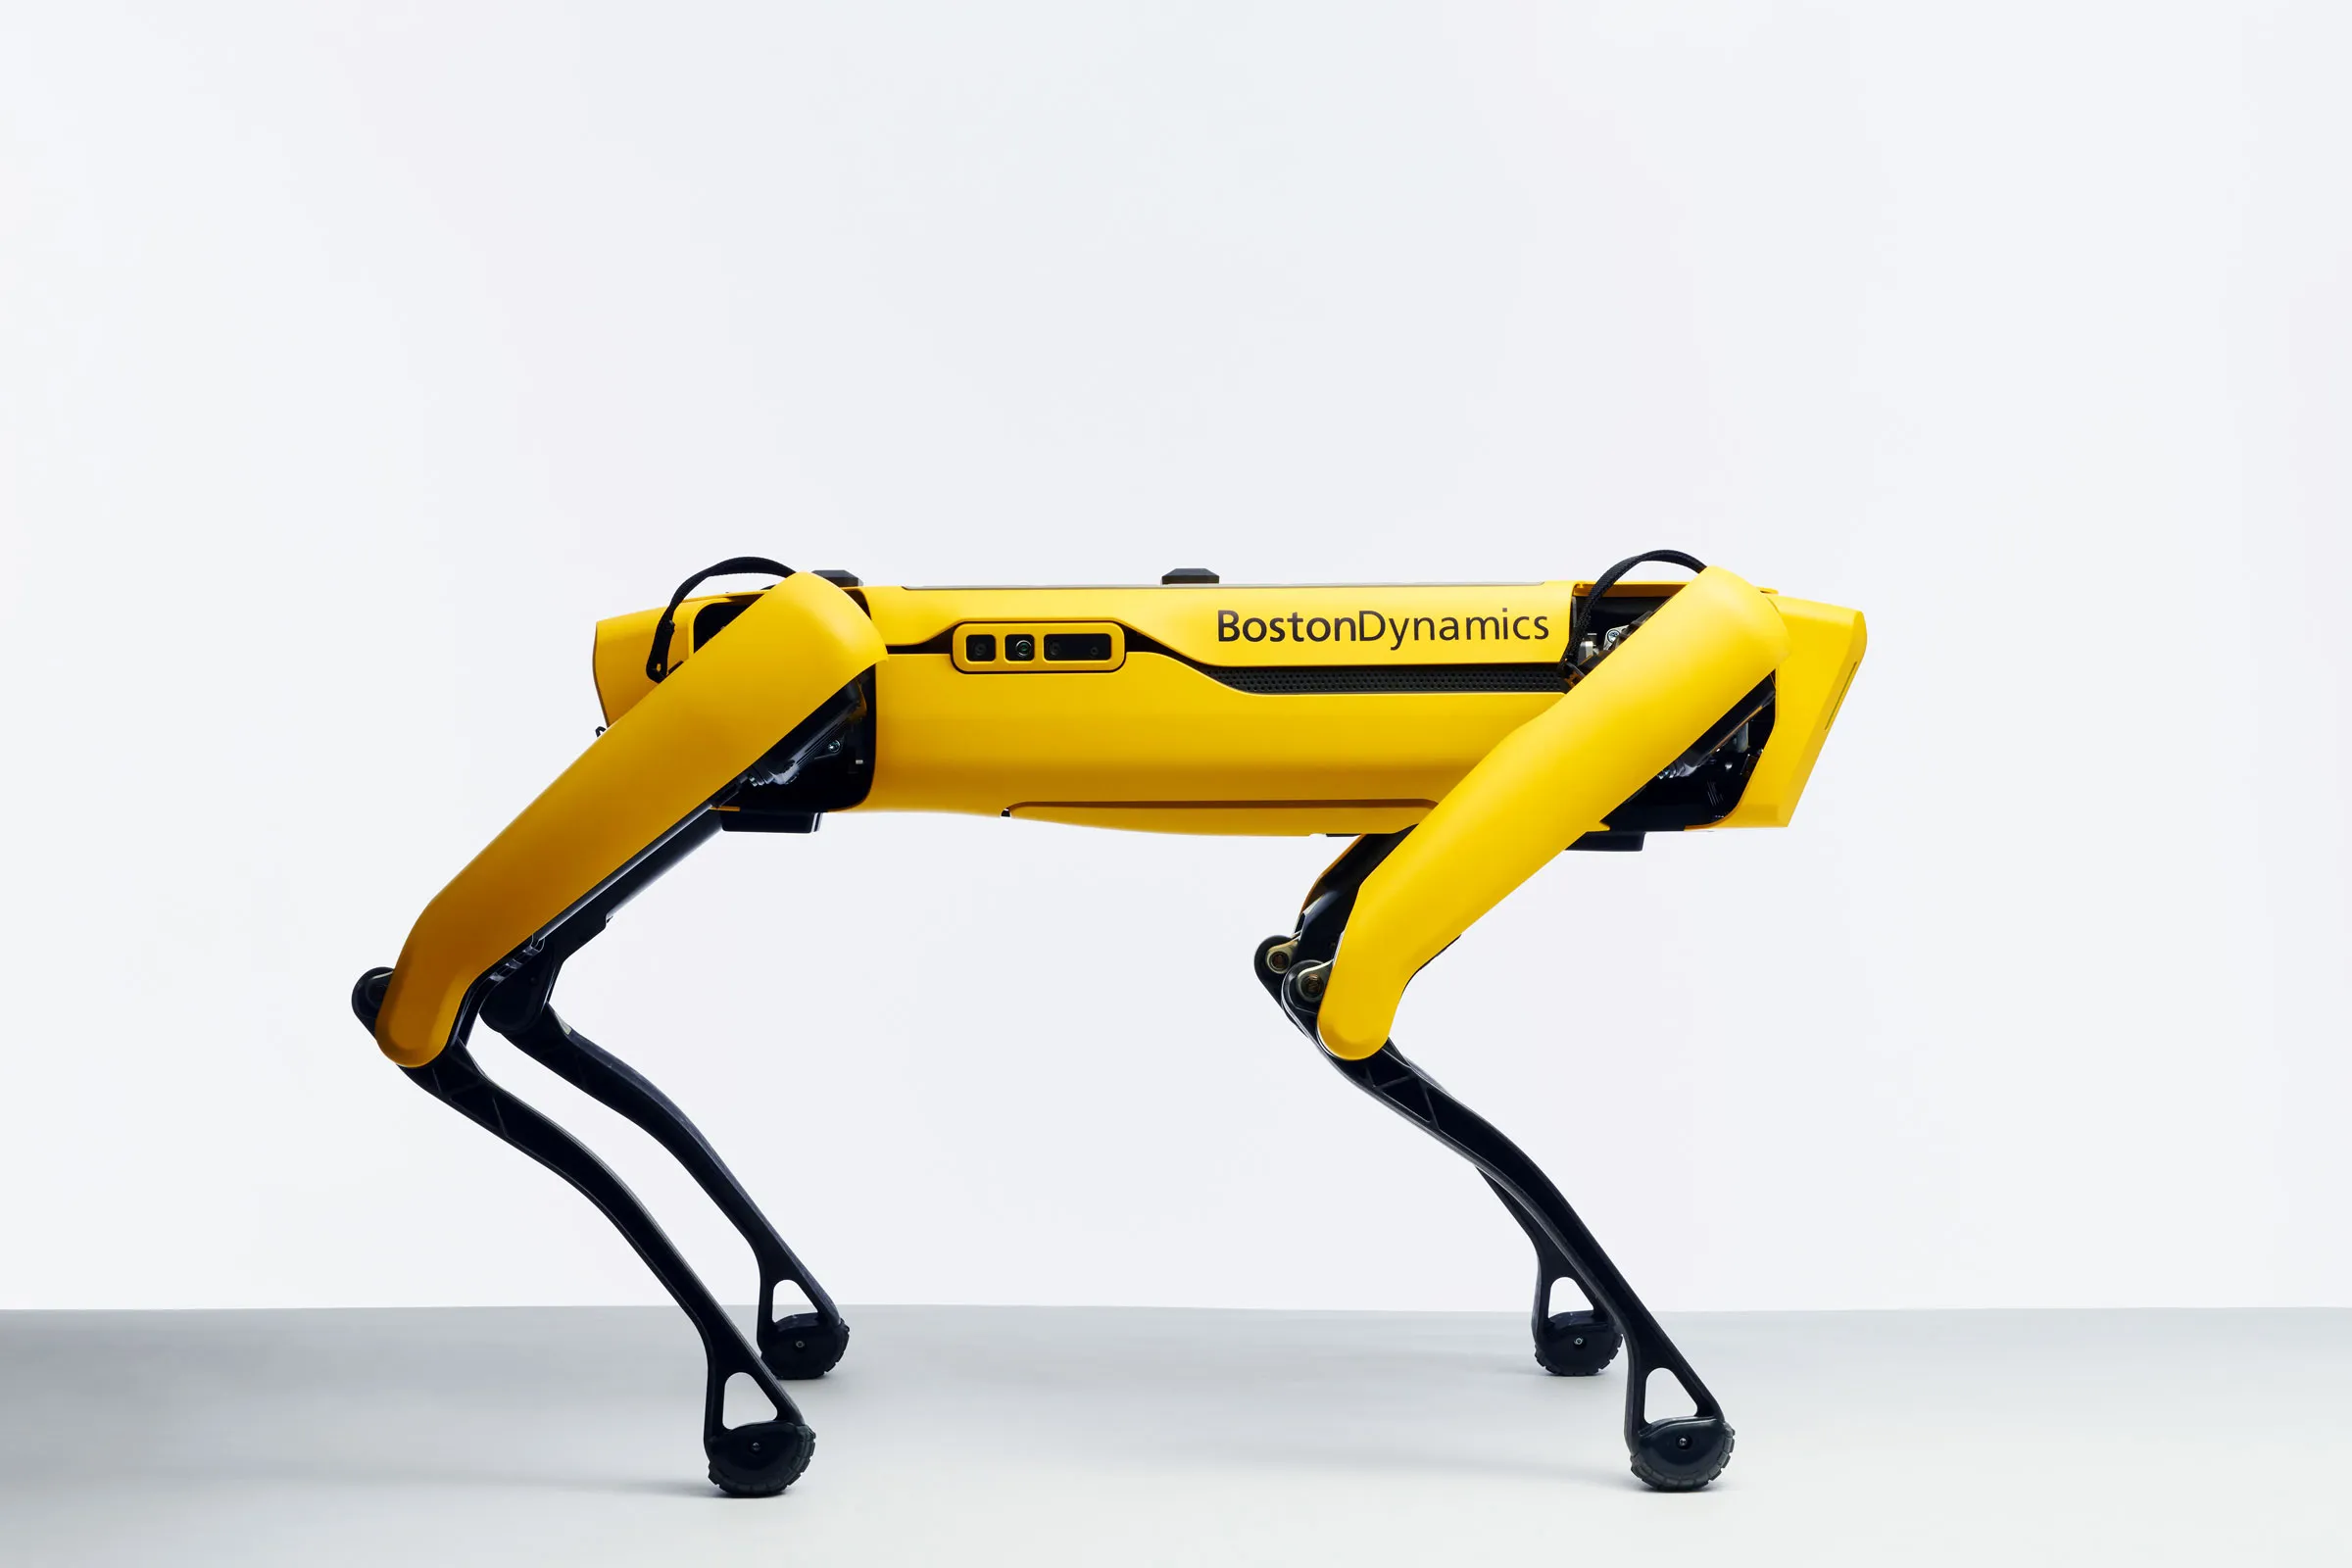
\includegraphics[width=0.7\textwidth]{hardware/robot_overview.png}
    \caption{Ví dụ robot bốn chân}
    \label{fig1}
\end{figure}

\section{Phân loại cấu trúc chân robot}
Cấu trúc cơ khí của chân robot có ảnh hưởng lớn đến khả năng điều khiển, hiệu suất chuyển động, độ chính xác cũng như khả năng mở rộng trong thiết kế. Dựa trên nguyên lý cơ học, cấu trúc chân robot có thể được chia thành ba loại chính: cấu trúc nối tiếp (Serial), cấu trúc song song (Parallel) và cấu trúc lai (Hybrid).

\textbf{\textit{Cấu trúc nối tiếp (Serial)}} 

Là cấu trúc phổ biến nhất, trong đó các khớp được liên kết tuần tự từ gốc (khung thân robot) đến điểm cuối (bàn chân). Mỗi khớp điều khiển một bậc tự do (DOF) và ảnh hưởng trực tiếp đến toàn bộ các khâu phía sau trong chuỗi động học. Hình \ref{fig8} minh họa một dạng cấu trúc chân nối tiếp với ba động cơ được gắn lần lượt tại khớp vai, khớp hông và khớp gối:

\begin{figure}[H]
    \centering
    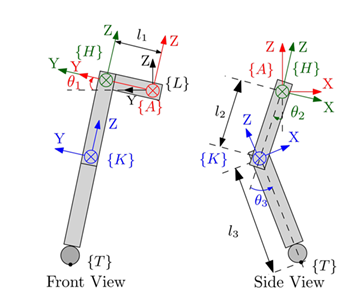
\includegraphics[width=0.6\textwidth]{hardware/serial_leg_both_sides.png}
    \caption{Cơ cấu chân dạng nối tiếp}
    \label{fig8}
\end{figure}

\textbf{\textit{Cấu trúc song song (Parallel)}} 

Trong cấu trúc này, nhiều nhánh cơ cấu hoạt động đồng thời để điều khiển một điểm cuối duy nhất, tạo nên hệ thống động học khép kín. Loại này thường có cấu hình tương tự như bệ Stewart (một dạng bệ lục giác có khung đồng bộ với các chân), mang lại độ cứng vững cao và độ chính xác chuyển động tốt hơn so với cấu trúc nối tiếp. Tuy nhiên, cấu trúc này có khối lượng cơ khí lớn và thuật toán tính toán động học thuận (FK), động học nghịch (IK) phức tạp hơn đáng kể. Hình \ref{fig9} trình bày một dạng cấu trúc chân song song phổ biến:

\begin{figure}[H]
    \centering
    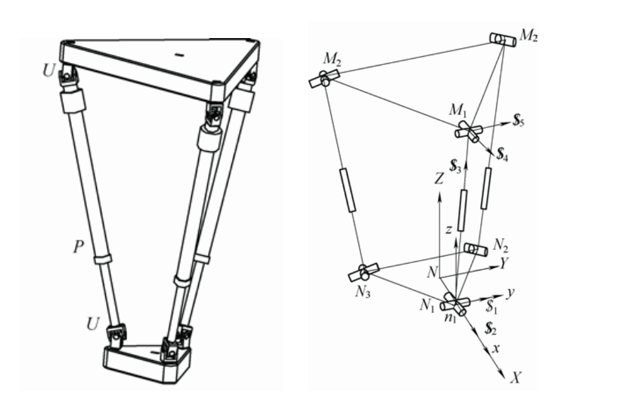
\includegraphics[width=0.6\textwidth]{hardware/mechanical_model.png }
    \caption{Mô hình cơ khí và hệ tọa độ nhánh của chân song song}
    \label{fig9}
\end{figure}

\textbf{\textit{Cấu trúc lai (Serial-Parallel Hybrid)}} 

Là sự kết hợp ưu điểm của cả hai cấu trúc trên, trong đó hệ thống sử dụng chuỗi động học nối tiếp để điều khiển chuyển động chính, đồng thời tích hợp cơ cấu song song để hỗ trợ truyền động (thường ứng dụng để dẫn động từ xa cho khớp gối). Do kết hợp cả hai cơ chế, phần chân robot thường nặng nề về mặt cơ khí và thuật toán điều khiển chuyển động cũng trở nên vô cùng phức tạp. Hình \ref{fig10} mô phỏng một trong những cấu trúc chân lai đơn giản nhất:

\begin{figure}[H]
    \centering
    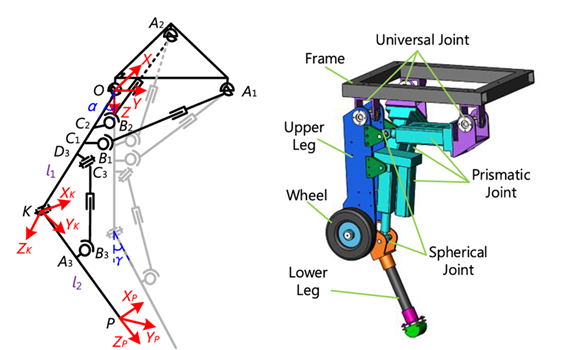
\includegraphics[width=0.6\textwidth]{hardware/mechanical_model_branch.png  }
    \caption{Cơ cấu chân lai nối tiếp – song song}
    \label{fig10}
\end{figure}

Sau quá trình đánh giá, nhằm tối ưu hóa trọng lượng phần cứng và tập trung vào phát triển giải thuật điều khiển cũng như thuận lợi cho việc kiểm chứng mô phỏng, cấu trúc chân nối tiếp (Serial) đã được lựa chọn cho nguyên mẫu robot.
\section{Cấu trúc liên kết động học của robot bốn chân}
Mặc dù tồn tại nhiều dạng cấu trúc liên kết động học khác nhau trong thiết kế robot bốn chân, các cấu hình với 8, 12 hoặc 16 bậc tự do (DOF) được sử dụng phổ biến nhất.

Cấu trúc 8 bậc tự do bao gồm bốn khớp hông và bốn khớp gối, trong đó tất cả các trục khớp song song với nhau. Robot 8 DOF có khả năng di chuyển tiến và lùi với tốc độ cao và tương đối dễ điều khiển do không có bậc tự do vung ngang tại khớp hông. Tuy nhiên, robot bốn chân 8 DOF không thể thực hiện chuyển động theo phương ngang và khả năng quay hướng bị hạn chế đáng kể, dẫn đến hiệu suất chuyển động không cao.

Ngược lại, robot bốn chân 16 DOF có số lượng khớp nhiều hơn, cho phép thực hiện các chuyển động linh hoạt và khéo léo hơn, nhưng đồng thời làm tăng đáng kể độ phức tạp trong điều khiển và tính toán.

Dựa trên những phân tích trên, cấu hình 12 bậc tự do, với mỗi chân gồm ba khớp quay, được lựa chọn cho thiết kế trong nghiên cứu này.

Về cấu hình chân, các dạng phổ biến bao gồm: inner knee-elbow, outer knee-elbow, full-knee và full-elbow. Hai cấu hình đầu có cấu trúc chân đối xứng hoàn toàn, do đó giúp robot đạt được độ ổn định cao hơn. Trong khi đó, hai cấu hình sau cung cấp không gian làm việc lớn hơn và thuận lợi hơn cho việc điều khiển chuyển động. Vì vậy, trong nghiên cứu này, cấu hình full-elbow được lựa chọn.

Cấu trúc liên kết động học kết cấu rút gọn được thể hiện ở Hình \ref{fig11}, trong đó khớp hông có hai bậc tự do quay (vung ngang và vung dọc), còn khớp gối có thêm một bậc tự do quay.

\begin{figure}[H]
    \centering
    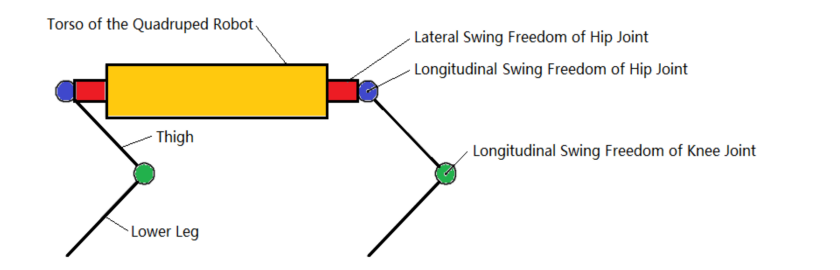
\includegraphics[width=0.6\textwidth]{hardware/structure_topology_front.png }
    \caption{Cấu trúc liên kết động học của robot bốn chân 12 bậc tự do}
    \label{fig11}
\end{figure}

\section{Cơ cấu chân 3 bậc tự do}
Đối với robot bốn chân, cơ cấu chân 3 bậc tự do được ưu tiên sử dụng phổ biến nhất nhờ tính linh hoạt cao trong việc mô phỏng các dáng đi sinh học. Một chân robot tiêu chuẩn thường được chia thành ba khâu chính: hông (\textit{hip}), đùi (\textit{thigh}) và cẳng chân (\textit{calf} hoặc \textit{lower thigh}). 

\begin{figure}[H]
    \centering
    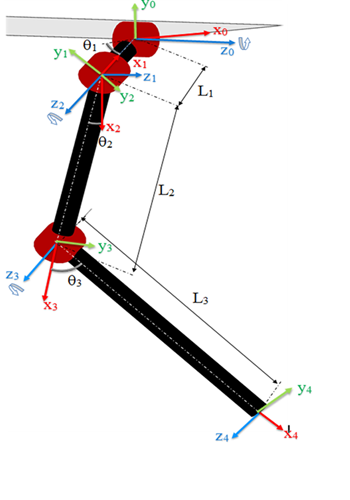
\includegraphics[width=0.6\textwidth]{kinematics/single_leg_3dof.png}
    \caption{Ba bậc tự do của cơ cấu một chân}
    \label{fig2}
\end{figure}

Như vậy, để cấu thành nên một robot bốn chân hoàn chỉnh, hệ thống sẽ cần tổng cộng 12 bậc tự do. Mỗi khớp tương ứng với một bậc tự do và được dẫn động độc lập bởi một động cơ. Sự phối hợp đồng bộ giữa 3 khớp này cho phép đầu bàn chân di chuyển đến bất kỳ tọa độ $(x, y, z)$ nào trong không gian làm việc của nó. Để đảm bảo sự đồng đều về lực, các động cơ được sử dụng thường có công suất định mức và mô-men xoắn tương đương nhau.

\section{Không gian làm việc }
Không gian làm việc chân robot là vùng không gian mà đầu bàn chân có thể vươn tới. Không gian làm việc của chân có thể được xác định bằng phương pháp phân tích hình học khi đã biết giới hạn góc quay của các động cơ và các khớp.

Phương pháp động học thuận rất hữu ích trong việc xác định không gian làm việc vì cơ cấu chân điển hình có cấu trúc tương tự như một tay máy nối tiếp. Đối với cơ cấu chân 3 bậc tự do với các giới hạn góc $\theta_{i,min} \leq \theta_i \leq \theta_{i,max}$ ($i = 1, 2, 3$), không gian làm việc được xác định bằng cách quét toàn bộ miền góc khớp cho phép và tính tọa độ đầu chân bằng FK:

\begin{equation}
    \mathbf{p}_{foot} = \text{FK}(\theta_1, \theta_2, \theta_3)
\end{equation}

Kết quả quét tạo ra một đám mây điểm 3D có dạng \textit{vòng cung} (annular sector), đặc trưng cho cơ cấu serial. Tầm với tối đa của chân đạt được khi các khâu duỗi thẳng ($\theta_3 = 0$):

\begin{equation}
    r_{max} = l_2 + l_3
\end{equation}

trong khi tầm với tối thiểu xảy ra khi các khâu gập hoàn toàn:

\begin{equation}
    r_{min} = |l_2 - l_3|
\end{equation}

Không gian làm việc có ý nghĩa quan trọng trong thiết kế: nó xác định phạm vi chiều cao đứng, chiều dài bước và biên độ chuyển động của robot. Vùng đạt được rộng nhất nằm trong mặt phẳng sagittal ($X$-$Z$), trong khi chiều ngang theo phương $Y$ bị giới hạn bởi biên độ khớp hông (hip - $\theta_1$).



\section{Các phương thức di chuyển}
Robot bốn chân có rất nhiều phương thức di chuyển khác nhau tùy thuộc vào tốc độ và đặc điểm địa hình. Dưới đây là 5 dáng đi (\textit{gait}) phổ biến nhất được áp dụng trong kỹ thuật điều khiển robot.

\textbf{\textit{Dáng đi Trot (Chạy kiệu)}} 

Đây là dáng đi phổ biến nhất và cũng là dáng đi trọng tâm được tác giả lựa chọn để thực hiện. Ở dáng đi này, hai chân chéo nhau (ví dụ: chân trước-trái và chân sau-phải) sẽ đồng thời nhấc lên và tiếp đất cùng lúc. \textit{Trot gait} giúp robot di chuyển nhanh và mượt mà, nhưng đòi hỏi bài toán điều khiển cân bằng động liên tục do đa giác chân đế thu hẹp lại thành một đường chéo.
    
\begin{figure}[H]
    \centering
    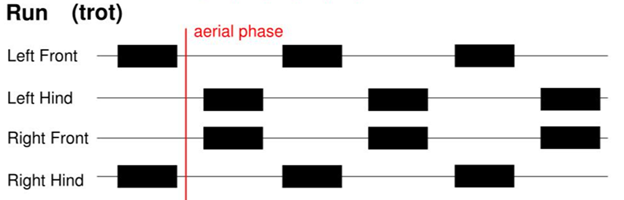
\includegraphics[width=0.6\textwidth]{gait_planner/trot_gait_table.png}
    \caption{Giản đồ pha chuyển động của dáng đi Trot}
    \label{fig3}
\end{figure}

\textbf{\textit{Dáng đi Walk (Đi bộ)}} 

Là dáng đi chậm và ổn định nhất. Tại bất kỳ thời điểm nào, robot luôn có ít nhất 3 chân tiếp đất để tạo thành một chân đế vững chắc, trong khi 1 chân được nhấc lên bước tới. Các pha (\textit{phase}) của 4 chân thường lệch nhau một góc $90^\circ$ (tương ứng $0^\circ, 90^\circ, 180^\circ, 270^\circ$).
    
\begin{figure}[H]
    \centering
    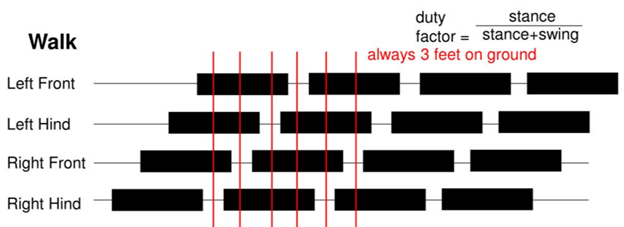
\includegraphics[width=0.6\textwidth]{gait_planner/walk_gait_table.png}
    \caption{Giản đồ pha chuyển động của dáng đi Walk}
    \label{fig4}
\end{figure}

\textbf{\textit{Dáng đi Pace (Đi kiệu song song)}} 

Hai chân cùng một bên (trái hoặc phải) được nhấc lên và tiến về phía trước cùng lúc. Đặc điểm của dáng đi này là trọng tâm khối lượng (CoM - \textit{Center of Mass}) của robot sẽ bị lắc lư ngang theo trục Y trong quá trình di chuyển, do đó hệ thống cần có cơ chế bù trừ thăng bằng tốt.
    
\begin{figure}[H]
    \centering
    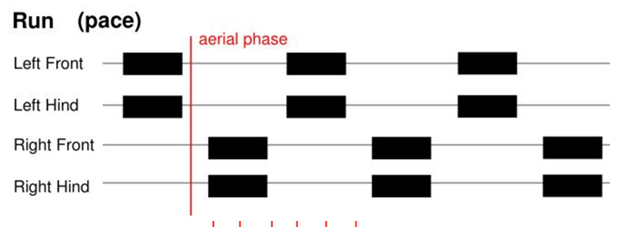
\includegraphics[width=0.6\textwidth]{gait_planner/pace_gait_table.png}
    \caption{Giản đồ pha chuyển động của dáng đi Pace}
    \label{fig5}
\end{figure}

\textbf{\textit{Dáng đi Bound (Nhảy vọt)}} 

Hai chân trước đồng thời nhấc lên vươn tới, ngay sau đó hai chân sau cũng nhấc lên tạo ra chuyển động nảy bật về phía trước, mô phỏng chuyển động của các loài thú săn mồi.
    
\begin{figure}[H]
    \centering
    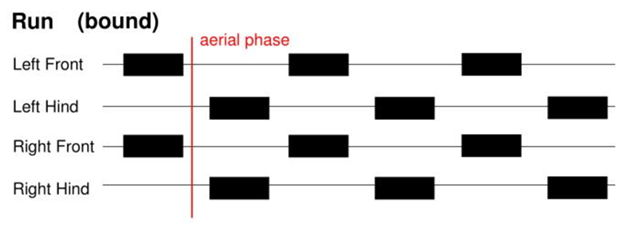
\includegraphics[width=0.6\textwidth]{gait_planner/bound_gait_table.png}
    \caption{Giản đồ pha chuyển động của dáng đi Bound}
    \label{fig6}
\end{figure}

\textbf{\textit{Dáng đi Gallop (Phi mã)}} 

Đây là dáng đi có tốc độ cao nhất của robot bốn chân. Quá trình di chuyển sẽ xuất hiện các pha bay hoàn toàn trên không (\textit{flight phase}), tức là không có chân nào chạm đất. Dáng đi này đòi hỏi các cơ cấu chấp hành có mô-men xoắn và tốc độ cực kỳ cao.
    
\begin{figure}[H]
    \centering
    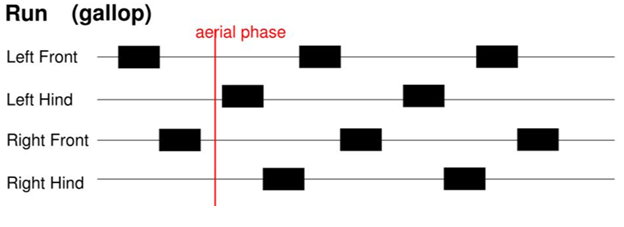
\includegraphics[width=0.6\textwidth]{gait_planner/gallop_gait_table.png}
    \caption{Giản đồ pha chuyển động của dáng đi Gallop}
    \label{fig7}
\end{figure}

\section{Lý thuyết ổn định cho robot có chân}

Phân tích ổn định là yêu cầu thiết yếu trong thiết kế và vận hành robot bốn chân. Khác với robot bánh xe có diện tích tiếp xúc liên tục với mặt đất, robot có chân chỉ tiếp xúc tại các điểm rời rạc, và diện tích đỡ thay đổi liên tục theo thời gian khi các chân chuyển pha.

\subsection{Ổn định tĩnh}

Robot có chân được xem là ổn định tĩnh tại một thời điểm nếu hình chiếu của trọng tâm (Center of Mass -- CoM) xuống mặt đất nằm bên trong đa giác đỡ (support polygon) --- đa giác lồi được tạo bởi các điểm tiếp xúc giữa các chân đang chạm đất và mặt đất.

\textbf{\textit{Biên ổn định tĩnh}} 

(Static Stability Margin -- SSM) được định nghĩa là khoảng cách nhỏ nhất từ hình chiếu CoM đến các cạnh của đa giác đỡ \cite{gonzalez2018}:

\begin{equation}
    \text{SSM} = \min_{i} \, d(\mathbf{p}_{CoM}, \overline{P_i P_{i+1}})
\end{equation}

trong đó $\mathbf{p}_{CoM}$ là hình chiếu CoM lên mặt đất, $\overline{P_i P_{i+1}}$ là cạnh thứ $i$ của đa giác đỡ, và $d(\cdot, \cdot)$ là khoảng cách từ điểm đến đoạn thẳng. Nếu SSM $> 0$, robot ổn định tĩnh; nếu SSM $\leq 0$, robot sẽ đổ.

\textbf{\textit{Ứng dụng cho dáng đi Trot}} 

Trong dáng đi trot, tại mỗi thời điểm có hai chân chéo nhau chạm đất. Đa giác đỡ suy biến thành một đoạn thẳng nối hai bàn chân. Về mặt lý thuyết, điều này có nghĩa là robot đang ở trạng thái biên của ổn định tĩnh (SSM $\approx 0$ khi CoM nằm đúng trên đoạn thẳng). Trong thực tế, diện tích tiếp xúc hữu hạn của bàn chân và quán tính của thân robot tạo ra một vùng ổn định hẹp nhưng đủ để duy trì chuyển động.

\begin{figure}[H]
    \centering
    \begin{subfigure}[b]{0.48\textwidth}
        \centering
        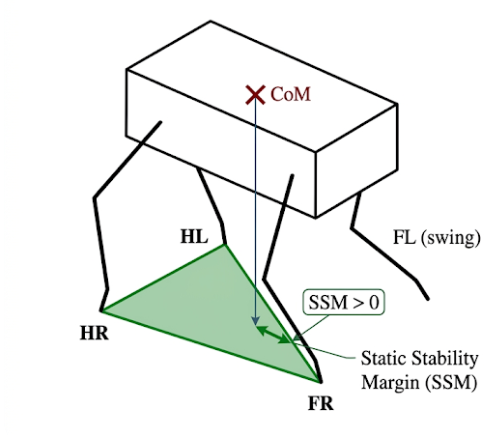
\includegraphics[width=\textwidth]{kinematics/static_stability_a.png}
        \caption{Walk Gait -- 3 stance legs}
    \end{subfigure}
    \hfill
    \begin{subfigure}[b]{0.48\textwidth}
        \centering
        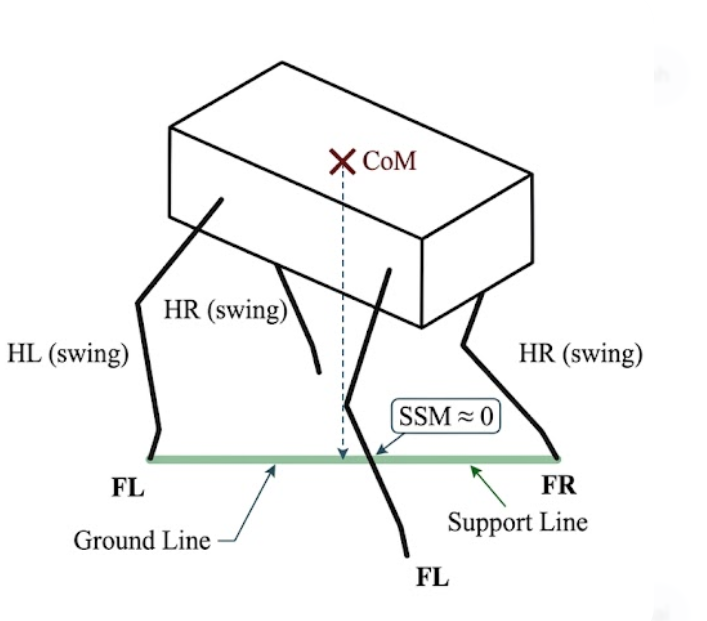
\includegraphics[width=\textwidth]{kinematics/static_stability_b.png}
        \caption{Trot Gait -- 2 diagonal stance legs}
    \end{subfigure}
    \caption{Minh họa Đa giác đỡ và Biên ổn định tĩnh (SSM) của robot bốn chân}
    \label{fig:static_stability}
\end{figure}

Trong nghiên cứu này, robot hoạt động ở tốc độ thấp với dáng đi Trot nên phân tích ổn định tĩnh là đủ cho mục đích thiết kế. Bộ điều khiển PID cân bằng kết hợp phản hồi IMU đóng vai trò bổ sung, giảm thiểu sai lệch hướng của thân robot khi di chuyển, chủ động đưa trọng tâm về gần đường nối hai bàn chân đang chạm đất.

\section{Lý thuyết bộ điều khiển PID}

Bộ điều khiển PID (Proportional--Integral--Derivative) là một trong những thuật toán điều khiển phản hồi được sử dụng rộng rãi và hiệu quả nhất trong kỹ thuật tự động hóa \cite{astrom2006}. Cấu trúc sơ đồ khối lý thuyết của bộ điều khiển PID được thể hiện trong Hình~\ref{fig:pid_theory_diagram}. Bộ điều khiển liên tục tính toán giá trị sai lệch $e(t) = r(t) - y(t)$ giữa giá trị đặt (setpoint) $r(t)$ và giá trị đo được (process variable) $y(t)$, sau đó áp dụng tín hiệu hiệu chỉnh dựa trên ba thành phần tỷ lệ, tích phân và vi phân.

\begin{figure}[H]
    \centering
    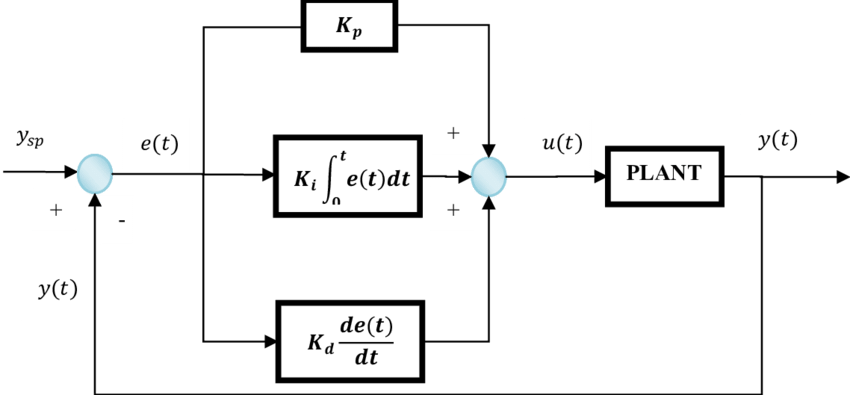
\includegraphics[width=0.8\textwidth]{architecture/Proportional-Integral-Derivative.png}
    \caption{Cấu trúc sơ đồ khối của bộ điều khiển PID}
    \label{fig:pid_theory_diagram}
\end{figure}

\subsection{Luật điều khiển PID chuẩn}

Tín hiệu điều khiển tổng hợp $u(t)$ trong miền thời gian liên tục được biểu diễn bằng phương trình:

\begin{equation}
    u(t) = K_P \cdot e(t) + K_I \int_{0}^{t} e(\tau)\,d\tau + K_D \frac{de(t)}{dt}
    \label{eq:pid_continuous}
\end{equation}

trong đó $K_P$, $K_I$, và $K_D$ lần lượt là hệ số khuếch đại tỷ lệ, hệ số tích phân và hệ số vi phân. Mỗi thành phần đóng một vai trò riêng biệt trong việc định hình đáp ứng của hệ thống. Trước hết, thành phần tỷ lệ (Proportional - P) tạo ra tín hiệu hiệu chỉnh tỷ lệ thuận với sai lệch hiện tại; hệ số $K_P$ càng lớn, hệ thống phản ứng càng nhanh nhưng đồng thời có xu hướng dao động và độ vọt lố (overshoot) cao. Thành phần P đơn thuần không thể triệt tiêu hoàn toàn sai lệch ở trạng thái xác lập. Tiếp theo, thành phần tích phân (Integral - I) tích lũy sai lệch theo thời gian để triệt tiêu hoàn toàn sai số ở trạng thái xác lập (steady-state error). Tuy nhiên, khi sai lệch tồn tại trong thời gian dài do hệ thống bị bão hòa cơ cấu chấp hành, giá trị tích phân tích lũy quá lớn sẽ gây ra hiện tượng bão hòa tích phân (\textit{integral windup}), khiến hệ thống bị vọt lố nghiêm trọng và phục hồi chậm. Cuối cùng, thành phần vi phân (Derivative - D) dự đoán xu hướng thay đổi của sai lệch dựa trên đạo hàm. Thành phần này hoạt động như một ``phanh'' hãm, giúp giảm vọt lố và cải thiện thời gian xác lập, mặc dù nhược điểm chính của khâu D là rất nhạy cảm với nhiễu tần số cao trong tín hiệu đo đạc từ cảm biến.

\subsection{Dạng rời rạc và triển khai số}

Trong các hệ thống vi điều khiển nhúng với chu kỳ lấy mẫu $\Delta t$, bộ điều khiển PID không thể tính toán các phép vi phân và tích phân liên tục. Do đó, phương trình \ref{eq:pid_continuous} được chuyển đổi thành dạng rời rạc (discrete-time):

\begin{equation}
    u_k = K_P \cdot e_k + K_I \sum_{j=0}^{k} e_j \cdot \Delta t + K_D \frac{e_k - e_{k-1}}{\Delta t}
    \label{eq:pid_discrete}
\end{equation}

trong đó chỉ số $k$ biểu thị bước thời gian hiện tại. Phương trình trên là dạng triển khai cơ bản nhất. Tuy nhiên, để đảm bảo hệ thống thực tế hoạt động ổn định và tin cậy, các kỹ thuật cải tiến thường được áp dụng thêm.

\subsection{Các cải tiến PID trong hệ thống thực}

Trong điều kiện vận hành thực tế, đặc biệt đối với robot bốn chân chịu ảnh hưởng lớn từ nhiễu động học và giới hạn phần cứng, bộ điều khiển PID cơ bản (phương trình \ref{eq:pid_discrete}) không thể đáp ứng tốt. Dựa trên mô hình MATLAB/Simulink và thực nghiệm, chuỗi điều khiển PID trong nghiên cứu này được tích hợp các cơ chế cải tiến sau:

\textbf{\textit{Bộ lọc trung bình trượt (EMA - Exponential Moving Average)}}

Trong quá trình di chuyển (chế độ GAIT), thân robot luôn dao động tuần hoàn. Nếu bộ điều khiển lấy mốc thăng bằng tuyệt đối (0 rad), nó sẽ liên tục sinh ra tín hiệu chống lại chính nhịp bước tự nhiên của robot. Việc áp dụng bộ lọc EMA tạo ra một đường cơ sở động (dynamic baseline):
\begin{equation}
    \text{Baseline}_k = \alpha_{ema} \cdot \text{Baseline}_{k-1} + (1 - \alpha_{ema}) \cdot y_k
\end{equation}
Sai lệch đưa vào PID sẽ là $e_k = \text{Baseline}_k - y_k$, giúp bộ điều khiển bỏ qua các dao động tự nhiên và chỉ phản ứng khi thân robot thực sự mất trọng tâm.

\textbf{\textit{Vùng chết (Deadband)}}

Cảm biến IMU luôn tồn tại nhiễu nhỏ ngay cả khi hệ thống ở vị trí cân bằng. Vùng chết triệt tiêu các sai lệch không đáng kể này để tránh động cơ phải bù trừ liên tục (chatter), giảm mài mòn cơ khí và tiết kiệm năng lượng:
\begin{equation}
    e_{dz} = \begin{cases}
        e - d & \text{nếu } e > d \\
        0 & \text{nếu } |e| \leq d \\
        e + d & \text{nếu } e < -d
    \end{cases}
\end{equation}
trong đó $d$ là bán kính của vùng chết.

\textbf{\textit{Chống bão hòa (Anti-windup) và Rò rỉ tích phân (Integral Leakage)}}

Để ngăn khâu tích phân (I) giữ lại các sai số cũ quá lâu hoặc bị bão hòa khi đạt giới hạn cơ cấu chấp hành, hệ số rò rỉ $\lambda \in (0, 1)$ được áp dụng để làm giảm dần giá trị tích phân theo thời gian (hàm mũ):
\begin{equation}
    \mathcal{I}_k = \lambda \cdot \mathcal{I}_{k-1} + e_k \cdot \Delta t
\end{equation}
Đồng thời, giá trị $\mathcal{I}_k$ được khống chế cứng (clamping) trong khoảng $[-\mathcal{I}_{max}, \mathcal{I}_{max}]$ nhằm đảm bảo an toàn.

\textbf{\textit{Reset tích phân tại giao điểm không (Zero-Crossing Reset)}}

Trong chế độ di chuyển tuần hoàn như dáng đi Trot, thân robot lắc qua lại liên tục qua trục cân bằng. Để tránh khâu tích phân gây ra quá điều chỉnh (overshoot) khi đổi chiều, hệ thống sẽ tự động xóa giá trị tích lũy ($\mathcal{I}_k = 0$) ngay khi sai số $e_k$ đổi dấu (vượt qua giao điểm không).

\textbf{\textit{Bão hòa đầu ra và Lọc thông thấp (Saturation \& Output LPF)}}

Tín hiệu hiệu chỉnh từ PID có thể chứa các gai nhiễu (chủ yếu từ khâu D). Trước khi xuất xuống hệ thống động học, tín hiệu được giới hạn biên độ chặt chẽ ($[-u_{max}, u_{max}]$) để không phá vỡ quỹ đạo sải bước nguyên vẹn. Sau đó, tín hiệu tiếp tục đi qua bộ lọc thông thấp (Low-Pass Filter) để làm mượt, đảm bảo động cơ vận hành êm ái, tránh hiện tượng trượt chân hoặc hụt bước.

\section{Cảm biến quán tính IMU và biểu diễn hướng}

\subsection{Nguyên lý hoạt động}

Bộ đo lường quán tính (Inertial Measurement Unit -- IMU) là thiết bị kết hợp nhiều loại cảm biến để đo gia tốc, vận tốc góc và hướng của vật thể trong không gian ba chiều. Một IMU tiêu chuẩn 9 trục thường bao gồm ba thành phần chính \cite{madgwick2011}. Thứ nhất là gia tốc kế (Accelerometer) dùng để đo gia tốc tuyến tính theo ba trục ($a_x, a_y, a_z$), bao gồm cả thành phần gia tốc trọng trường; từ các phép đo này, góc nghiêng tĩnh (roll, pitch) có thể được suy ra thông qua hướng của vector trọng lực. Thứ hai là con quay hồi chuyển (Gyroscope) làm nhiệm vụ đo vận tốc góc ($\omega_x, \omega_y, \omega_z$) quanh ba trục; mặc dù việc tích phân vận tốc góc theo thời gian cho ra góc quay, do sai số tích lũy (drift), phương pháp này không đáng tin cậy trong thời gian dài. Cuối cùng là từ kế (Magnetometer) có chức năng đo cường độ từ trường Trái Đất theo ba trục, cung cấp thông tin về hướng Bắc từ, từ đó cho phép hệ thống xác định góc hướng (yaw).

\subsection{Biểu diễn hướng: Quaternion và góc Euler}

Hướng của một vật rắn trong không gian ba chiều có thể được biểu diễn bằng nhiều phương pháp, trong đó phổ biến nhất là góc Euler và quaternion.

\textbf{\textit{Góc Euler}} 

Sử dụng ba góc quay liên tiếp quanh các trục cố định hoặc trục động để mô tả hướng. Trong hệ quy ước ZYX (yaw--pitch--roll), ma trận xoay tổng hợp là:

\begin{equation}
    R = R_z(\psi) \cdot R_y(\theta) \cdot R_x(\phi)
\end{equation}

trong đó $\phi$ là góc lăn (roll), $\theta$ là góc nghiêng (pitch), và $\psi$ là góc hướng (yaw). Nhược điểm chính của biểu diễn Euler là hiện tượng khóa gimbal (gimbal lock), xảy ra khi $\theta = \pm 90^\circ$, khiến hai trục quay trùng nhau và mất một bậc tự do.

\textbf{\textit{Quaternion}} 

$\mathbf{q} = (w, x, y, z)$ với $|\mathbf{q}| = 1$ biểu diễn phép quay một góc $\alpha$ quanh trục đơn vị $\hat{n} = (n_x, n_y, n_z)$:

\begin{equation}
    \mathbf{q} = \left(\cos\frac{\alpha}{2},\; n_x \sin\frac{\alpha}{2},\; n_y \sin\frac{\alpha}{2},\; n_z \sin\frac{\alpha}{2}\right)
\end{equation}

Quaternion không bị hiện tượng khóa gimbal, tính toán nội suy mượt mà hơn, và yêu cầu ít phép toán hơn so với ma trận xoay. Công thức chuyển đổi từ quaternion sang góc Euler thường dùng trong robotics là:

\begin{align}
    \phi   &= \text{atan2}\left(2(w x + y z),\; 1 - 2(x^2 + y^2)\right) \\
    \theta &= \arcsin\left(2(w y - z x)\right) \\
    \psi   &= \text{atan2}\left(2(w z + x y),\; 1 - 2(y^2 + z^2)\right)
\end{align}

\subsection{Bộ lọc cảm biến}

Dữ liệu thô từ IMU chứa nhiễu tần số cao và sai số trôi (drift), do đó cần được xử lý qua bộ lọc trước khi sử dụng. Có nhiều phương pháp phổ biến được ứng dụng trong thực tế. Khái niệm cơ bản nhất là bộ lọc bổ sung (Complementary Filter), kết hợp dữ liệu gia tốc kế (tin cậy ở tần số thấp) và con quay hồi chuyển (tin cậy ở tần số cao) thông qua hệ số trọng số $\alpha$:
\begin{equation}
    \hat{\theta}_k = \alpha \cdot (\hat{\theta}_{k-1} + \omega_k \Delta t) + (1-\alpha) \cdot \theta_{acc,k}
\end{equation}
Bên cạnh đó, bộ lọc Kalman là một phương pháp ước lượng tối ưu dựa trên mô hình trạng thái, kết hợp dự đoán (prediction) từ mô hình động học với cập nhật (update) từ phép đo. Trong đó, bộ lọc Kalman mở rộng (EKF) thường được sử dụng cho các hệ phi tuyến. Một giải pháp thay thế hiệu quả là bộ lọc Madgwick \cite{madgwick2011}, một thuật toán tính toán nhẹ sử dụng quy hoạch gradient (gradient descent) để tối ưu hóa quaternion ước lượng, rất phù hợp với các hệ thống nhúng có tài nguyên hạn chế. Hiện nay, giải pháp tối ưu hóa phần cứng là sử dụng Sensor Fusion tích hợp (On-chip); một số module IMU cao cấp như BNO055 được tích hợp sẵn bộ xử lý sensor fusion để tính toán và cung cấp trực tiếp quaternion hoặc góc Euler đã được lọc nhiễu, giúp giảm đáng kể khối lượng tính toán cho vi xử lý chính.

\section{Tổng quan về nền tảng ROS~2 và Gazebo}

ROS~2 (Robot Operating System 2) \cite{ros2docs} là nền tảng phần mềm mã nguồn mở cung cấp kiến trúc truyền thông phân tán thời gian thực dựa trên middleware DDS. Việc sử dụng ROS~2 cho phép chia nhỏ các tác vụ điều khiển robot thành các Node độc lập (ví dụ: Node tính toán động học, Node điều khiển cân bằng) giao tiếp lỏng ghép với nhau thông qua cơ chế Publish/Subscribe, qua đó tăng cường độ tin cậy và khả năng mở rộng của hệ thống.

Song song với ROS~2, Gazebo \cite{gazebo} được sử dụng làm môi trường mô phỏng vật lý 3D. Nhờ khả năng tích hợp chặt chẽ với ROS~2 và hỗ trợ mô phỏng động lực học chính xác (trọng lực, ma sát, va chạm), đồ án áp dụng quy trình phát triển ``sim-to-real''. Thuật toán điều khiển và mô hình URDF của robot được kiểm thử toàn diện trên Gazebo để loại trừ các lỗi logic trước khi triển khai xuống máy tính nhúng và cơ cấu chấp hành thực tế, giúp tiết kiệm thời gian và đảm bảo an toàn phần cứng.


Mục tiêu của bài toán động học thuận của robot là xác định biểu diễn vị trí của cơ cấu chấp hành cuối. Trong nghiên cứu này, phương pháp biến đổi tọa độ Modified Denavit--Hartenberg (MD-H) \cite{denavit1955, craig2005} được áp dụng để giải quyết bài toán này.
\section{Mô hình động học}
\subsection{Thiết lập hệ tọa độ MD-H}

Nhóm xây dựng một mô hình toán học và cơ khí của robot bốn chân phân bố trong không gian Descartes. Cấu trúc vật lý của robot bao gồm kích thước bệ đỡ với chiều dài $L=209$ mm, chiều rộng $W=191$ mm, và chiều dài các khâu chân lần lượt là $L_1=26$ mm (Coxa/Hip), $L_2=106$ mm (Femur/Thigh), và $L_3=125$ mm (Tibia/Calf).

\begin{figure}[H]
    \centering
    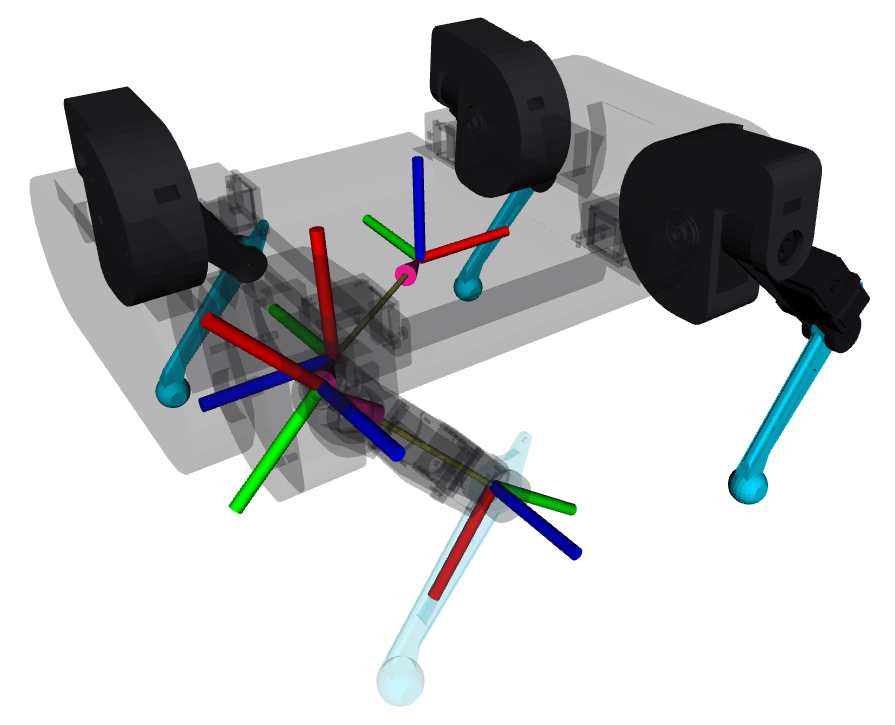
\includegraphics[width=0.7\textwidth]{kinematics/model_reference_frame.png}
    \caption{Mô hình mô phỏng với các hệ tọa độ tham chiếu được gắn tại từng khớp của robot.}
    \label{fig20}
\end{figure}

Theo quy ước chuẩn của hệ điều hành ROS (Robot Operating System), các trục tọa độ trong Hình \ref{fig20} được biểu diễn bằng màu sắc: Trục $X$ (Đỏ) chỉ hướng tiến về phía trước, Trục $Y$ (Xanh lá) chỉ hướng sang trái, và Trục $Z$ (Xanh dương) chỉ hướng lên trên. Các hệ tọa độ cấu thành nên mô hình động học MD-H của chân được gắn cụ thể trên hình, bao gồm: Hệ tọa độ thân $\{B\}$, cụm khớp hông (Roll và Pitch) đại diện bởi $\{0\}, \{1\}, \{2\}$, khớp gối $\{3\}$ và mũi bàn chân $\{4\}$.

Dựa theo hướng tiến về phía trước, chân trước bên trái (LF), chân trước bên phải (RF), chân sau bên trái (LB) và chân sau bên phải (RB) lần lượt được đánh số là 1, 2, 3 và 4. Hệ tọa độ thân $\{B\}$ (hoặc $\{O_B\}$) được thiết lập tại tâm hình học của thân, và hệ tọa độ gốc của chân $\{0\}$ (hoặc $\{O_{i,0}\}$) được thiết lập tại khớp nối giữa khớp hông và thân, trong đó $i = 1,2,3,4$.

Trong phương pháp biến đổi tọa độ Modified Denavit-Hartenberg (MD-H) \cite{craig2005}, chuỗi động học được mô tả một cách toán học thông qua các phép biến đổi tọa độ chính xác. Mỗi khâu liên kết được xác định bởi bốn tham số như trong Hình~\ref{fig21}, theo định nghĩa chuẩn của MD-H, bao gồm: $a_{i-1}$ là khoảng cách từ trục $Z_{i-1}$ đến trục $Z_i$ đo dọc theo trục $X_{i-1}$; $\alpha_{i-1}$ là góc quay từ trục $Z_{i-1}$ đến trục $Z_i$ đo quanh trục $X_{i-1}$; $d_i$ là khoảng cách từ trục $X_{i-1}$ đến trục $X_i$ đo dọc theo trục $Z_i$; và cuối cùng, $\theta_i$ là góc quay từ trục $X_{i-1}$ đến trục $X_i$ đo quanh trục $Z_i$.

\begin{figure}[H]
    \centering
    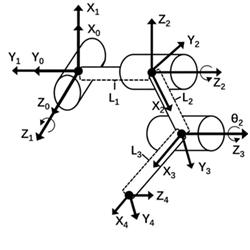
\includegraphics[width=0.6\textwidth]{kinematics/dh_coordinate_system.png }
    \caption{Mô hình một chân của robot bốn chân được xây dựng bằng phương pháp MD-H.}
    \label{fig21}
\end{figure}

Các tham số MD-H của từng khâu liên kết cho một chân robot được thiết lập và trình bày chi tiết trong Bảng \ref{tab:3}, phản ánh chính xác sự khác biệt về cấu trúc động học giữa các chân bên trái và bên phải (tham số $d_2$ mang dấu đối nhau do hệ quả của phép đối xứng gương).

\begin{table}[H]
\centering
\caption{Tham số Modified Denavit-Hartenberg (MD-H)}
\label{tab:3}
\renewcommand{\arraystretch}{1.4}
\begin{tabular}{l c c c c c}
\toprule
\textbf{Link ($i$)} & $\boldsymbol{\alpha_{i-1}}$ & $\boldsymbol{a_{i-1}}$ & \multicolumn{2}{c}{$\boldsymbol{d_i}$} & $\boldsymbol{\theta_i}$ \\
\cmidrule(lr){4-5}
& & & \textbf{Left Limbs} & \textbf{Right Limbs} & \\
\midrule
1 (Coxa)  & $0^\circ$ & $0$   & $0$    & $0$   & $\theta_1^*$ \\
2 (Femur) & $90^\circ$& $0$   & $L_1$  & $-L_1$& $\theta_2^*$ \\
3 (Tibia) & $0^\circ$ & $L_2$ & $0$    & $0$   & $\theta_3^*$ \\
4 (Foot)  & $0^\circ$ & $L_3$ & $0$    & $0$   & $0$ \\
\bottomrule
\multicolumn{6}{l}{\small $^*$ Variable articulation angle} \\
\end{tabular}
\end{table}

\subsection{Giải động học thuận}

Khi giải các phương trình động học thuận bằng phương pháp MD-H, chúng thường được 
phân rã thành các bài toán con. Phép biến đổi từ hệ tọa độ khâu $\{i-1\}$ sang hệ 
tọa độ $\{i\}$ tạo ra một ma trận biến đổi tọa độ chỉ liên quan đến bốn tham số 
liên kết $^{i-1}_{i}T$. Dựa trên định nghĩa của từng tham số liên kết ở trên, ta có:

\begin{equation}
^{i-1}_{i}T = Trans_x\{a_{i-1}\} \, Rot_x\{\alpha_{i-1}\} \, Trans_z\{d_i\} \, Rot_z\{\theta_i\}
\end{equation}
\begin{equation}
{}^{i-1}_{i}T=
\begin{bmatrix}
\cos\theta_i & -\sin\theta_i & 0 & a_{i-1} \\
\sin\theta_i\cos\alpha_{i-1} & \cos\theta_i\cos\alpha_{i-1} & -\sin\alpha_{i-1} & -d_i\sin\alpha_{i-1} \\
\sin\theta_i\sin\alpha_{i-1} & \cos\theta_i\sin\alpha_{i-1} & \cos\alpha_{i-1} & d_i\cos\alpha_{i-1} \\
0 & 0 & 0 & 1
\end{bmatrix}
\end{equation}
Áp dụng cho cấu trúc của một chân robot, các ma trận biến đổi thành phần được xác định như sau:

\begin{equation}
{}^{0}_{1}T=
\begin{bmatrix}
\cos\theta_1 & -\sin\theta_1 & 0 & 0 \\
\sin\theta_1 & \cos\theta_1 & 0 & 0 \\
0 & 0 & 1 & 0 \\
0 & 0 & 0 & 1
\end{bmatrix}
\end{equation}

\begin{equation}
{}^{1}_{2}T=
\begin{bmatrix}
\cos\theta_2 & -\sin\theta_2 & 0 & 0 \\
0 & 0 & -1 & -L_1 \\
\sin\theta_2 & \cos\theta_2 & 0 & 0 \\
0 & 0 & 0 & 1
\end{bmatrix}
\end{equation}

\begin{equation}
{}^{2}_{3}T=
\begin{bmatrix}
\cos\theta_3 & -\sin\theta_3 & 0 & L_2 \\
\sin\theta_3 & \cos\theta_3 & 0 & 0 \\
0 & 0 & 1 & 0 \\
0 & 0 & 0 & 1
\end{bmatrix}
\end{equation}

\begin{equation}
{}^{3}_{4}T=
\begin{bmatrix}
1 & 0 & 0 & L_3 \\
0 & 1 & 0 & 0 \\
0 & 0 & 1 & 0 \\
0 & 0 & 0 & 1
\end{bmatrix}
\end{equation}
Theo Hình \ref{fig20}, ma trận biến đổi từ hệ tọa độ $\{O_{i,0}\}$ đến hệ tọa độ thân $\{O_B\}$ được viết như sau:

\begin{equation}
^{B}_{0}T=
\begin{bmatrix}
0 & 0 & 1 & \frac{L}{2} \\
0 & -1 & 0 & \frac{W}{2} \\
1 & 0 & 0 & 0 \\
0 & 0 & 0 & 1
\end{bmatrix}
\end{equation}

Do đó, ma trận biến đổi của hệ tọa độ đầu chân so với hệ tọa độ thân $\{O_B\}$ được xác định như sau:

\begin{equation}
^{B}_{4}T = {}^{B}_{0}T \, {}^{0}_{4}T
\end{equation}

\begin{equation}
{}^{B}_{4}T =
\begin{bmatrix}
S_{23} & c_{23} & 0 & \frac{L}{2} + L_2 S_2 + L_3 S_{23} \\
- S_1 c_{23} & S_1 S_{23} & c_1 & \frac{W}{2} + L_1 c_1 - L_2 S_1 c_2 - L_3 S_1 c_{23} \\
c_1 c_{23} & - c_1 S_{23} & S_1 & L_1 S_1 + L_2 c_1 c_2 + L_3 c_1 c_{23} \\
0 & 0 & 0 & 1
\end{bmatrix}
\end{equation}

\begin{equation}
{}^{B}_{4}T=
\begin{bmatrix}
R & P \\
0 & 1
\end{bmatrix}
\end{equation}

\begin{equation}
{}^{B}_{4}T=
\begin{bmatrix}
 &  &  & P_x \\
 & R &  & P_y \\
 &  &  & P_z \\
0 & 0 & 0 & 1
\end{bmatrix}
\end{equation}

\begin{equation}
R=
\begin{bmatrix}
S_{23} & c_{23} & 0 \\
- S_1 c_{23} & S_1 S_{23} & c_1 \\
c_1 c_{23} & - c_1 S_{23} & S_1
\end{bmatrix}
\end{equation}

\begin{equation}
P =
\begin{bmatrix}
P_x^B \\
P_y^B \\
P_z^B
\end{bmatrix}
=
\begin{bmatrix}
\dfrac{L}{2}+L_2 s_2 + L_3 s_{23} \\
\dfrac{W}{2}+L_1 c_1 - L_2 s_1 c_2 - L_3 s_1 c_{23} \\
L_1 s_1 + L_2 c_1 c_2 + L_3 c_1 c_{23}
\end{bmatrix}
\end{equation}

\begin{equation}
P_{LF}=
\begin{bmatrix}
P_x \\
P_y \\
P_z
\end{bmatrix}
=
\begin{bmatrix}
L_1\sin\theta_1 + L_2\cos\theta_1\cos\theta_2 + L_3\cos\theta_1\cos(\theta_2+\theta_3) \\
- L_1\cos\theta_1 + L_2\sin\theta_1\cos\theta_2 + L_3\sin\theta_1\cos(\theta_2+\theta_3) \\
L_2\sin\theta_2 + L_3\sin(\theta_2+\theta_3)
\end{bmatrix}
\label{eq:1}
\end{equation}

\begin{equation}
P_{RF}=
\begin{bmatrix}
P_x \\
P_y \\
P_z
\end{bmatrix}
=
\begin{bmatrix}
- L_1\sin\theta_1 + L_2\cos\theta_1\cos\theta_2 + L_3\cos\theta_1\cos(\theta_2+\theta_3) \\
L_1\cos\theta_1 + L_2\sin\theta_1\cos\theta_2 + L_3\sin\theta_1\cos(\theta_2+\theta_3) \\
L_2\sin\theta_2 + L_3\sin(\theta_2+\theta_3)
\end{bmatrix}
\label{eq:2}
\end{equation}

\begin{equation}
P_{LB}=
\begin{bmatrix}
P_x \\
P_y \\
P_z
\end{bmatrix}
=
\begin{bmatrix}
L_1\sin\theta_1 + L_2\cos\theta_1\cos\theta_2 + L_3\cos\theta_1\cos(\theta_2+\theta_3) \\
- L_1\cos\theta_1 + L_2\sin\theta_1\cos\theta_2 + L_3\sin\theta_1\cos(\theta_2+\theta_3) \\
L_2\sin\theta_2 + L_3\sin(\theta_2+\theta_3)
\end{bmatrix}
\label{eq:3}
\end{equation}

\begin{equation}
P_{RB}=
\begin{bmatrix}
P_x \\
P_y \\
P_z
\end{bmatrix}
=
\begin{bmatrix}
- L_1\sin\theta_1 + L_2\cos\theta_1\cos\theta_2 + L_3\cos\theta_1\cos(\theta_2+\theta_3) \\
L_1\cos\theta_1 + L_2\sin\theta_1\cos\theta_2 + L_3\sin\theta_1\cos(\theta_2+\theta_3) \\
L_2\sin\theta_2 + L_3\sin(\theta_2+\theta_3)
\end{bmatrix}
\label{eq:4}
\end{equation}

Các ma trận trên biểu diễn vị trí mũi bàn chân của cả 4 chân trong hệ tọa độ cục bộ của từng khớp hông. Do tính chất đối xứng, phương trình động học của chân sau bên trái giống với chân trước bên trái, và chân sau bên phải giống với chân trước bên phải.

\section{Động học nghịch }

Bài toán động học nghịch (Inverse Kinematics -- IK) là bài toán xác định các giá trị góc khớp $(\theta_1, \theta_2, \theta_3)$ khi biết tọa độ đầu bàn chân $(x, y, z)$ trong hệ tọa độ thân robot. Đây là bài toán ngược của động học thuận, và thường có nhiều nghiệm (do tính phi tuyến của các phương trình lượng giác) hoặc không có nghiệm (khi điểm đích nằm ngoài không gian làm việc).

Trong nghiên cứu này, phương pháp giải tích (analytical method) được sử dụng để giải bài toán IK. Phương pháp này tận dụng cấu trúc chuỗi hở của chân robot để giải trực tiếp hệ phương trình lượng giác, từ đó thu được kết quả nhanh chóng và chính xác dạng đóng. Các bước tính toán chi tiết sẽ được trình bày cụ thể dưới đây.

Khi thiết kế phương trình động học nghịch cho robot bốn chân, một điểm đặc biệt cần lưu ý là các chân trái và chân phải được lắp ráp đối xứng nhau như hình ảnh qua gương. Do tính chất này, ta không thể áp dụng chung một công thức toán học y hệt nhau cho cả 4 chân. Cụ thể, có ba yếu tố vật lý tạo ra sự khác biệt. Thứ nhất là vị trí gắn chân trên thân; do mỗi chân được gắn ở một góc khác nhau, khoảng cách từ tâm robot đến các gốc chân có sự thay đổi về dấu, tương ứng với một nửa chiều dài ($\pm L/2$) và một nửa chiều rộng ($\pm W/2$). Thứ hai là cấu hình của khớp hông (Coxa); do lắp đặt đối xứng, với cùng một góc quay, chân trái và chân phải sẽ vung về hai hướng ngược nhau, do đó để công thức toán học tính đúng hướng, tham số chiều dài khâu hông $L_1$ sẽ mang dấu âm ($-L_1$) đối với các chân bên trái và mang dấu dương ($+L_1$) đối với các chân bên phải. Cuối cùng là cấu hình gập gối (Tibia); để duy trì hình dáng gập gối đồng nhất cho cả hai bên (để gối không bị bẻ ngược), toán hạng $\sin\theta_3$ bắt buộc phải nhận hai dấu trái ngược nhau giữa chân trái ($-$) và chân phải ($+$).

Thay vì phải xây dựng 4 hệ phương trình động học hoàn toàn độc lập, giải pháp tối ưu là thiết kế một bộ công thức tổng quát duy nhất. Sau đó, tùy thuộc vào việc đang tính toán cho chân nào, thuật toán chỉ việc tra bảng để đưa các hệ số dấu tương ứng vào công thức nhằm tìm ra góc khớp chính xác.

Cụ thể trong triển khai thực tế, hàm IK nhận tọa độ đầu bàn chân $(x_B, y_B, z_B)$ trong hệ tọa độ thân robot $\{O_B\}$. Dựa vào tính chất đối xứng trên, tọa độ này sẽ được biến đổi sang hệ tọa độ cục bộ của chân $(x', y', z')$ bằng cách cộng trừ các offset vị trí gốc chân tương ứng và hoán đổi trục cho phù hợp với quy ước MD-H. Phương trình biến đổi cho mỗi chân được viết như sau:

\begin{equation}
x' = z_B, \qquad
y' = \sigma_W \cdot \frac{W}{2} - y_B, \qquad
z' = \sigma_L \cdot \frac{L}{2} + x_B
\label{eq:body_to_leg}
\end{equation}

trong đó $\sigma_W$ và $\sigma_L$ là các hệ số dấu phụ thuộc vào vị trí chân, được trình bày trong Bảng~\ref{tab:ik_signs}.

\begin{table}[h]
\centering
\caption{Hệ số dấu biến đổi tọa độ và dấu IK cho bốn chân}
\label{tab:ik_signs}
\renewcommand{\arraystretch}{1.3}
\begin{tabular}{|l|c|c|c|c|}
\hline
\textbf{Chân} & $\sigma_W$ & $\sigma_L$ & Dấu $L_1$ trong $\theta_1$ & Dấu $\sin\theta_3$ \\ \hline
Left-Front  & $+1$ & $-1$ & $-L_1$ & $-1$ \\ \hline
Left-Behind & $+1$ & $+1$ & $-L_1$ & $-1$ \\ \hline
Right-Front & $-1$ & $-1$ & $+L_1$ & $+1$ \\ \hline
Right-Behind & $-1$ & $+1$ & $+L_1$ & $+1$ \\ \hline
\end{tabular}
\end{table}

\textbf{\textit{Quá trình giải hệ phương trình}} 

Sau khi biến đổi tọa độ, bài toán IK được giải thống nhất cho cả bốn chân thông qua bốn bước sau. Các hệ số dấu tham chiếu Bảng~\ref{tab:ik_signs}.

\textbf{\textit{Bước 1 -- Giải $\theta_1$}} 

Từ phép chiếu tọa độ $(x', y')$ lên mặt phẳng vuông góc với trục hip:
\begin{equation}
\theta_1 =
\mathrm{atan2}(-x',\, y')
+
\mathrm{atan2}
\left(
-\sqrt{x'^2 + y'^2 - L_1^2},\; \pm L_1
\right)
\label{eq:ik_theta1}
\end{equation}
trong đó dấu $\pm L_1$ là $-L_1$ cho chân trái và $+L_1$ cho chân phải.

\textbf{\textit{Bước 2 -- Tính biến trung gian}}
\begin{equation}
\begin{aligned}
p_1 &= x' \cos\theta_1 + y' \sin\theta_1 \\
p_2 &= \sigma_{p2} \cdot z'
\end{aligned}
\label{eq:ik_p1p2}
\end{equation}
trong đó $\sigma_{p2} = +1$ cho chân trái và $\sigma_{p2} = -1$ cho chân phải.

\textbf{\textit{Bước 3 -- Giải $\theta_3$}} 

Áp dụng định lý hàm số cosine:
\begin{equation}
\cos\theta_3 =
\frac{p_1^2 + p_2^2 - L_2^2 - L_3^2}{2 L_2 L_3}
\end{equation}

\begin{equation}
\sin\theta_3 =
\sigma_{s3} \sqrt{1 - \cos^2\theta_3}
\end{equation}

\begin{equation}
\theta_3 = \mathrm{atan2}(\sin\theta_3,\, \cos\theta_3)
\end{equation}
trong đó $\sigma_{s3} = -1$ cho chân trái và $\sigma_{s3} = +1$ cho chân phải, nhằm duy trì cấu hình gối đối xứng.

\textbf{\textit{Bước 4 -- Giải $\theta_2$}}
\begin{equation}
\theta_2 =
\mathrm{atan2}(p_2,\, p_1)
-
\mathrm{atan2}(L_3 \sin\theta_3,\, L_2 + L_3 \cos\theta_3)
\label{eq:ik_theta2}
\end{equation}

\section{Quy hoạch dáng đi và phân tích chuyển động }

Quy hoạch dáng đi đóng vai trò then chốt đối với sự di chuyển ổn định của robot bốn chân. Trong tự nhiên, các loài động vật có vú bốn chân lựa chọn các dáng đi khác nhau tùy thuộc vào vận tốc di chuyển mong muốn và độ gồ ghề của bề mặt địa hình nhằm giảm thiểu năng lượng tiêu thụ mà vẫn đạt được mục tiêu di chuyển. Trên cơ sở đó, các mẫu dáng đi phổ biến của động vật đã được trích xuất để làm nền tảng cho việc quy hoạch dáng đi trên robot bốn chân.

\subsection{Lựa chọn dáng đi Trot}
Dựa trên các phân tích lý thuyết về các phương thức di chuyển đã trình bày ở Chương 2, tác giả lựa chọn dáng đi \textbf{trot} làm trọng tâm nghiên cứu \cite{marhefka1999}. Đây là kiểu dáng đi ``hai nhịp'' điển hình, trong đó hai chân chéo nhau có đặc tính chuyển động giống hệt nhau, với chân trước bên trái (LF) và chân sau bên phải (RB) hoạt động đồng nhất, còn chân trước bên phải (RF) và chân sau bên trái (LB) hoạt động đồng nhất, như được thể hiện trong Hình~\ref{fig22}.

Về mặt lý thuyết, hệ số chu kỳ nhiệm vụ (duty cycle coefficient) trong dáng đi này không chịu bất kỳ hạn chế nào, và thỏa mãn điều kiện:
\begin{equation}
    0 < \beta < 1
\end{equation}
Do đó, robot có dải tốc độ rộng và có thể lựa chọn các tốc độ khác nhau cho các địa hình khác nhau. Ngoài ra, các thực nghiệm về lượng oxy tiêu thụ của ngựa ở các dáng đi khác nhau (walk, trot và gallop) cho thấy dáng đi trot có mức tiêu thụ năng lượng tương đối thấp trong một dải tốc độ khá lớn. Điều này chứng minh rằng dáng đi này có hiệu suất năng lượng cao về mặt lý thuyết.

\begin{figure}[H]
    \centering
    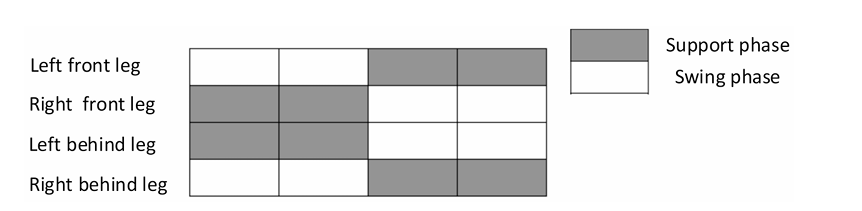
\includegraphics[width=0.6\textwidth]{gait_planner/trot_gait_timing.png}
    \caption{Sơ đồ thời gian của dáng đi trot với $\beta = 0.5$, trong đó $\beta = \frac{T_{st}}{T}$ và $T_{st}$ là thời gian của pha chống đỡ.}
    \label{fig22}
\end{figure}

Tùy thuộc vào giá trị của hệ số chu kỳ làm việc, dáng đi trot chéo 
có thể được chia thành ba loại.

Khi $\beta < 0.5$, robot xuất hiện một pha bay ngắn, tức là thời điểm 
mà cả bốn chân đều ở pha vung. Khi đó tốc độ di chuyển của robot tăng 
đáng kể, tuy nhiên sự xuất hiện của pha bay này cũng làm tăng đáng kể độ khó trong 
việc điều khiển.

Khi $\beta > 0.5$, robot có bốn giai đoạn chống đỡ khi chân vung chuyển 
đổi trạng thái. Điều này giúp tăng độ ổn định nhưng đồng thời làm giảm tốc độ di 
chuyển của robot.

Khi $\beta = 0.5$, hai cặp chân chéo luân phiên chuyển đổi liên tục giữa pha vung 
và pha chống đỡ. Trạng thái này nằm giữa hai trường hợp trên và đảm bảo sự cân 
bằng giữa tốc độ di chuyển và độ ổn định của robot, do đó đây là dáng đi được 
sử dụng phổ biến nhất.

\section{Quy hoạch quỹ đạo cho robot bốn chân}

Chuyển động của chân robot về cơ bản được mô tả thông qua quỹ đạo chuyển động của robot. 
Trong đó, quỹ đạo là sự biến thiên theo thời gian của vị trí, vận tốc và gia tốc 
của từng bậc tự do của robot.

Khi quá trình mô phỏng được thực hiện mà không có một phương pháp quy hoạch quỹ đạo phù hợp, 
chuyển động của robot thường trở nên ngẫu nhiên và không đều, đồng thời robot sẽ khó duy trì 
được sự cân bằng. Nguyên nhân của hiện tượng này là do sự thay đổi đột ngột của vận tốc trong 
không gian Descartes.

\begin{figure}[H]
    \centering
    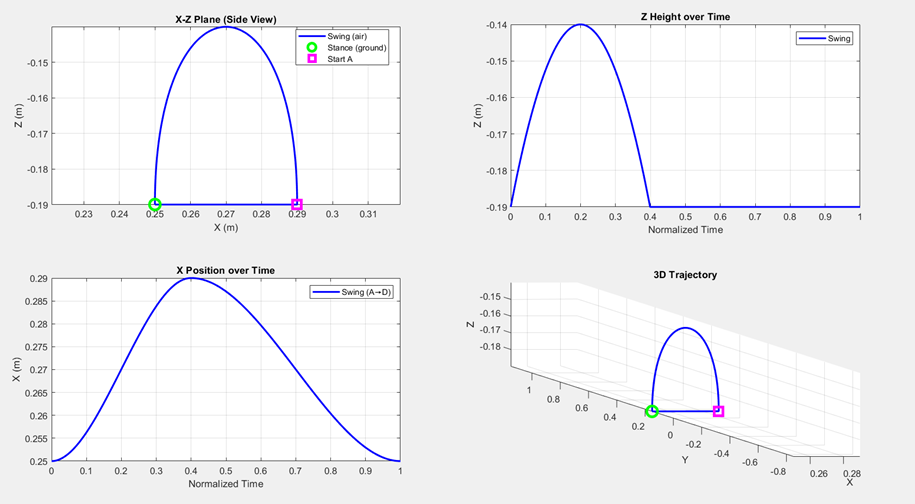
\includegraphics[width=0.6\textwidth]{gait_planner/single_leg_trajectory.png }
    \caption{Phân tích quỹ đạo của một chân}
    \label{fig23}
\end{figure}

Việc quy hoạch quỹ đạo là cần thiết cho quá trình phân tích chuyển động dựa trên 
động học. Do đó, quỹ đạo được tạo ra với sự hỗ trợ của các điểm trung gian nhằm 
duy trì dạng chuyển động mượt mà. Vì robot bốn chân có 3 bậc tự do nên chuyển 
động của robot có sự thay đổi trên cả ba trục trong không gian Descartes.

\subsection{Nội suy đa thức bậc ba}

Trong quá trình xây dựng quỹ đạo chuyển động, phương pháp nội suy đa thức thường được sử dụng để tạo ra đường cong chuyển 
động liên tục giữa các điểm. Một trong những phương pháp phổ biến là nội suy 
đa thức bậc ba. Dạng tổng quát của đa thức bậc ba được 
biểu diễn như sau:

\[
f(t) = a_3 t^3 + a_2 t^2 + a_1 t + a_0
\]

Trong đó $a_0, a_1, a_2, a_3$ là các hệ số được xác định dựa trên bốn điều kiện biên 
gồm vị trí và vận tốc tại các điểm đầu và cuối của quỹ đạo:

\begin{align}
x(0) &= x_0, \quad x(T) = x_f \\
\dot{x}(0) &= 0, \quad \dot{x}(T) = 0
\end{align}

Phương pháp này giúp tạo ra quỹ đạo liên tục và đảm bảo tính liên tục của vị trí và vận tốc 
trong quá trình chuyển động.

\begin{figure}[H]
    \centering
    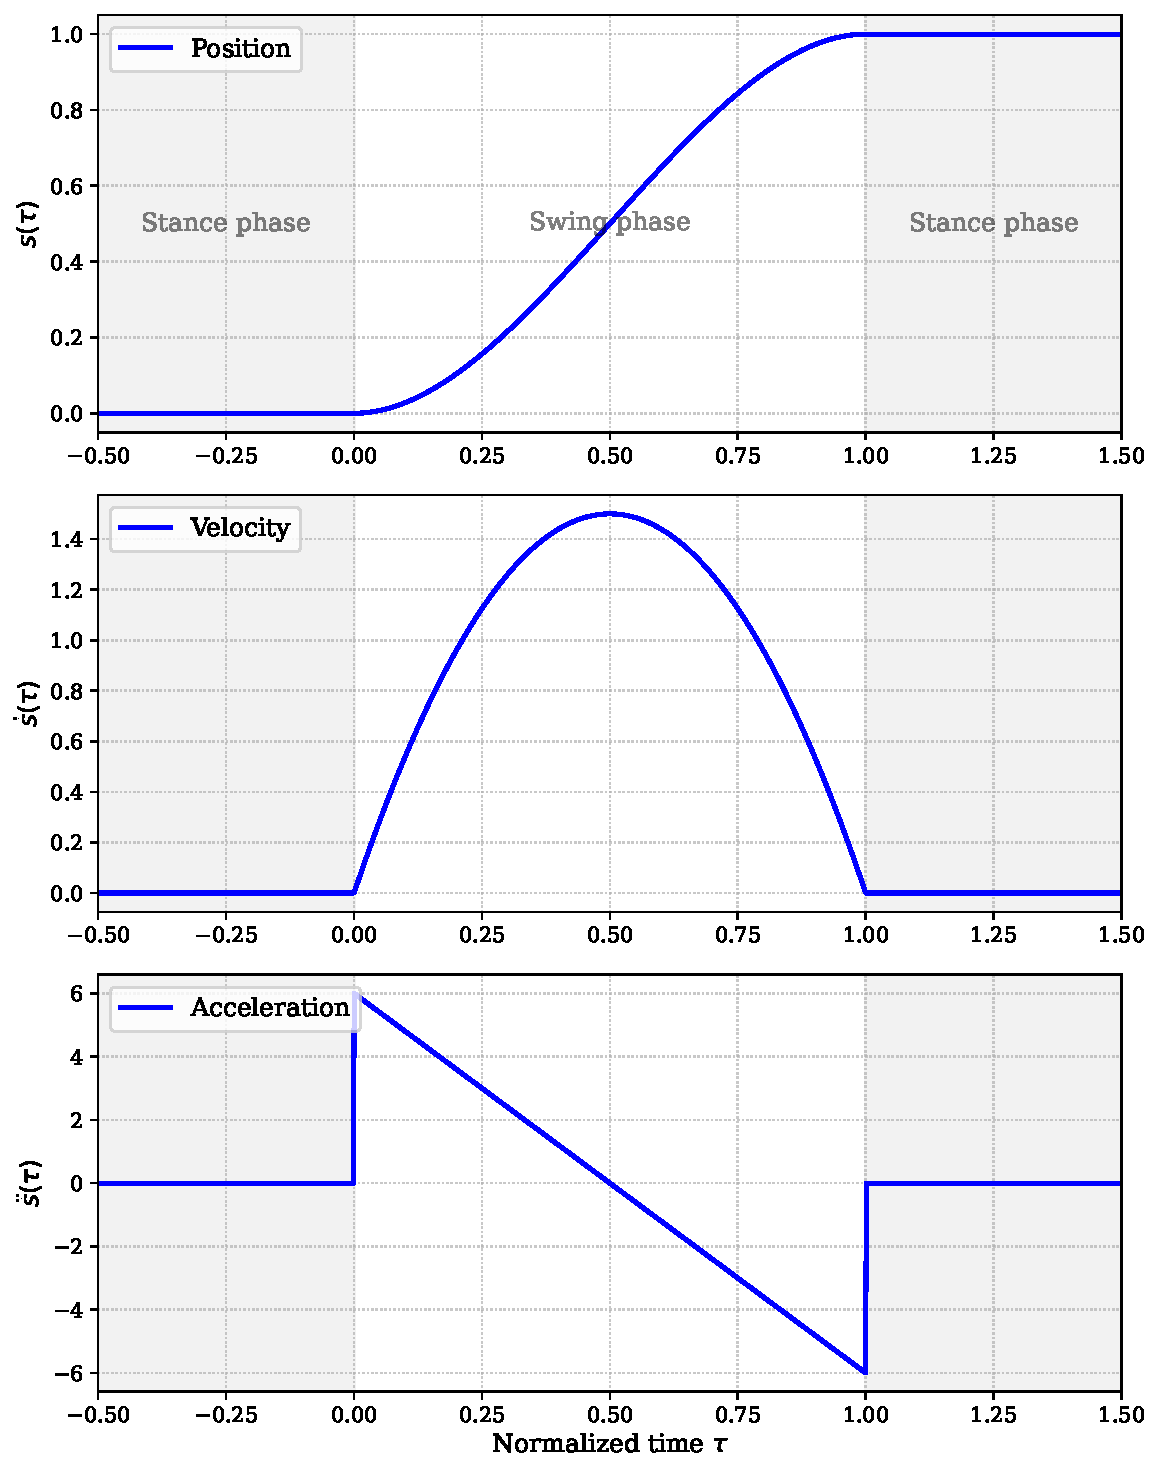
\includegraphics[width=0.8\textwidth]{gait_planner/cubic_pva.pdf}
    \caption{Các đường cong quỹ đạo bậc ba}
    \label{fig25}
\end{figure}

\subsection{Nội suy đa thức bậc năm}

Tuy nhiên, để cải thiện độ mượt của quỹ đạo và đảm bảo thêm điều kiện liên 
tục của gia tốc, phương pháp nội suy đa thức bậc năm được sử dụng. Dạng tổng quát:

\[
f(t) = a_5 t^5 + a_4 t^4 + a_3 t^3 + a_2 t^2 + a_1 t + a_0
\]

Các hệ số được xác định dựa trên sáu điều kiện biên gồm 
vị trí, vận tốc và gia tốc tại điểm đầu và điểm cuối:

\begin{align}
x(0) &= x_0, \quad x(T) = x_f \\
\dot{x}(0) &= 0, \quad \dot{x}(T) = 0 \\
\ddot{x}(0) &= 0, \quad \ddot{x}(T) = 0
\end{align}

Việc sử dụng đa thức bậc năm cho phép đảm bảo tính liên tục bậc hai ($C^2$) của vị trí, vận tốc và gia tốc, 
từ đó giúp chuyển động của robot trở nên ổn định và mượt mà hơn.

\begin{figure}[H]
    \centering
    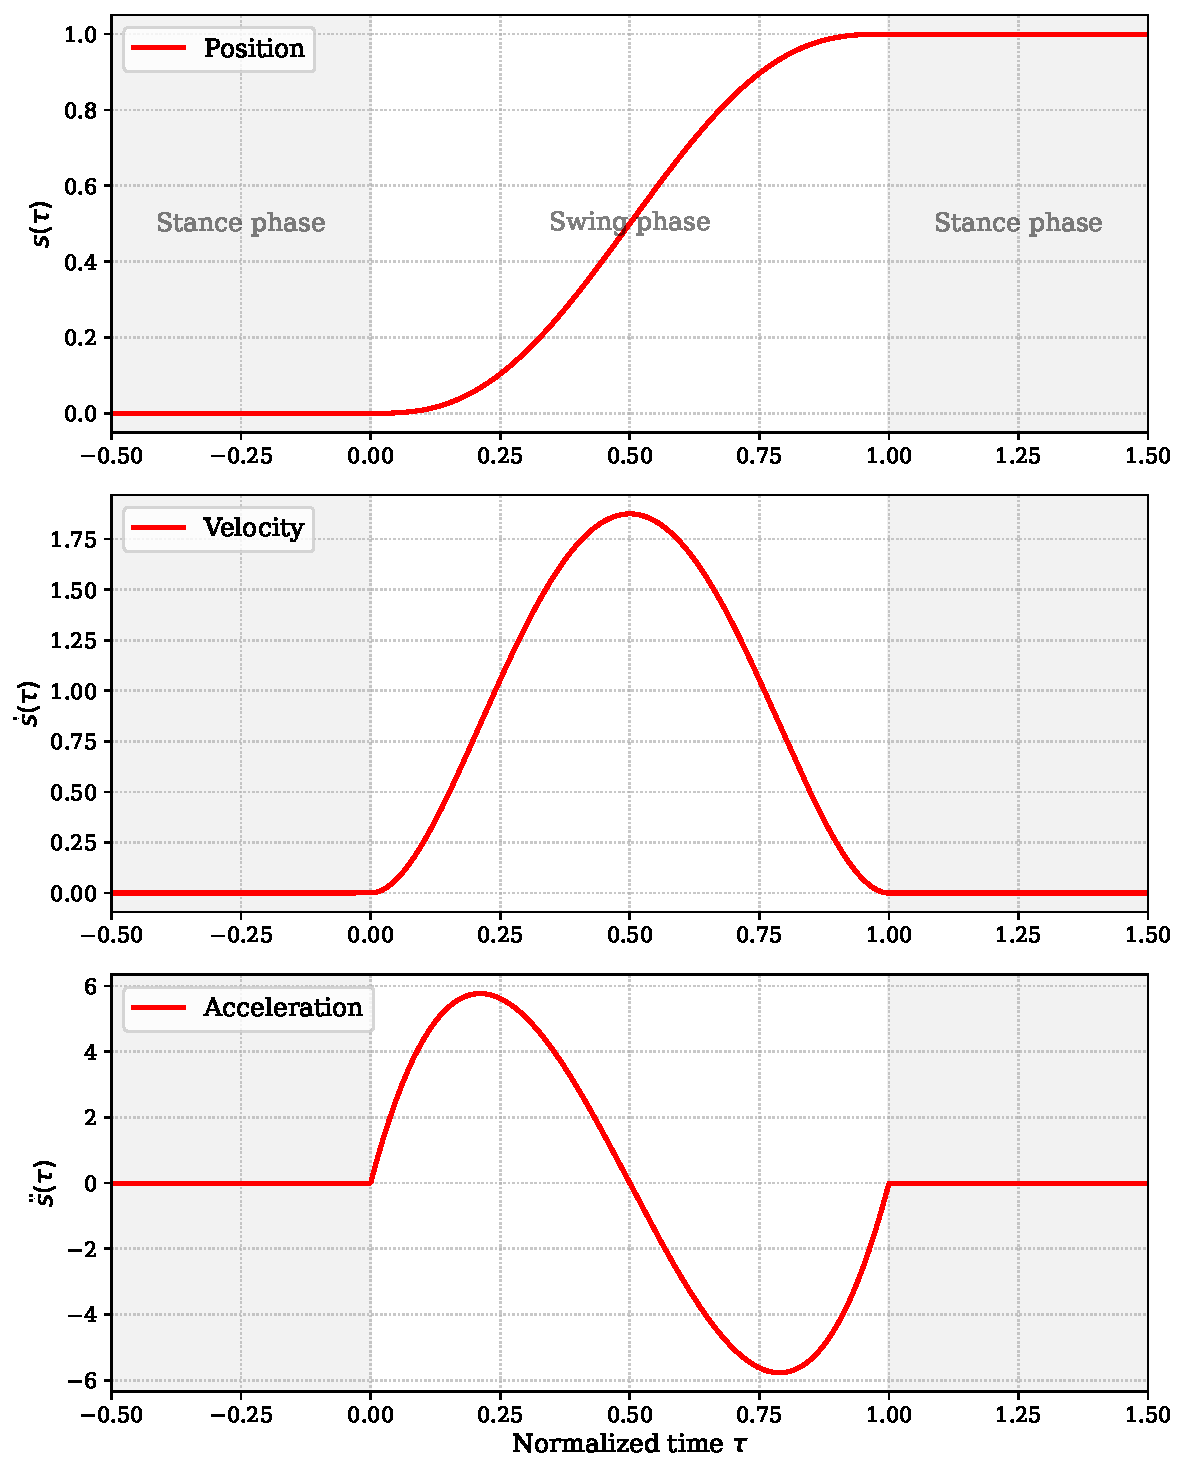
\includegraphics[width=0.8\textwidth]{gait_planner/quintic_pva.pdf}
    \caption{Biên dạng vị trí, vận tốc và gia tốc của hàm bước mượt bậc năm}
    \label{fig26}
\end{figure}

Khi giải hệ sáu phương trình với sáu ẩn, nghiệm dạng đóng thu được dưới dạng tham số chuẩn hóa. Đặt $\tau = t/T \in [0,\,1]$, hàm bước mượt bậc năm (quintic smooth-step) được xác định là:

\begin{equation}
s(\tau) = 10\tau^3 - 15\tau^4 + 6\tau^5
\label{eq:quintic_step}
\end{equation}

Hàm $s(\tau)$ thỏa mãn tất cả sáu điều kiện biên:

\begin{equation}
s(0) = 0,\; s(1) = 1,\quad \dot{s}(0) = \dot{s}(1) = 0,\quad \ddot{s}(0) = \ddot{s}(1) = 0
\end{equation}

Nhờ đó, quỹ đạo giữa hai điểm bất kỳ có thể được viết gọn:

\begin{equation}
\mathbf{p}(\tau) = \mathbf{p}_0 + s(\tau) \cdot (\mathbf{p}_f - \mathbf{p}_0)
\end{equation}

trong đó $\mathbf{p}_0$ và $\mathbf{p}_f$ lần lượt là vị trí đầu và vị trí cuối.

\subsection{So sánh nội suy bậc ba và bậc năm}

Để làm rõ lý do lựa chọn phương pháp đa thức bậc năm thay vì bậc ba, ta xét biểu đồ so sánh biên dạng vị trí, vận tốc và gia tốc của cả hai phương pháp trên cùng một khoảng thời gian chuẩn hóa $\tau \in [0,\,1]$ (Hình~\ref{fig:cubic_vs_quintic}).

\begin{figure}[H]
    \centering
    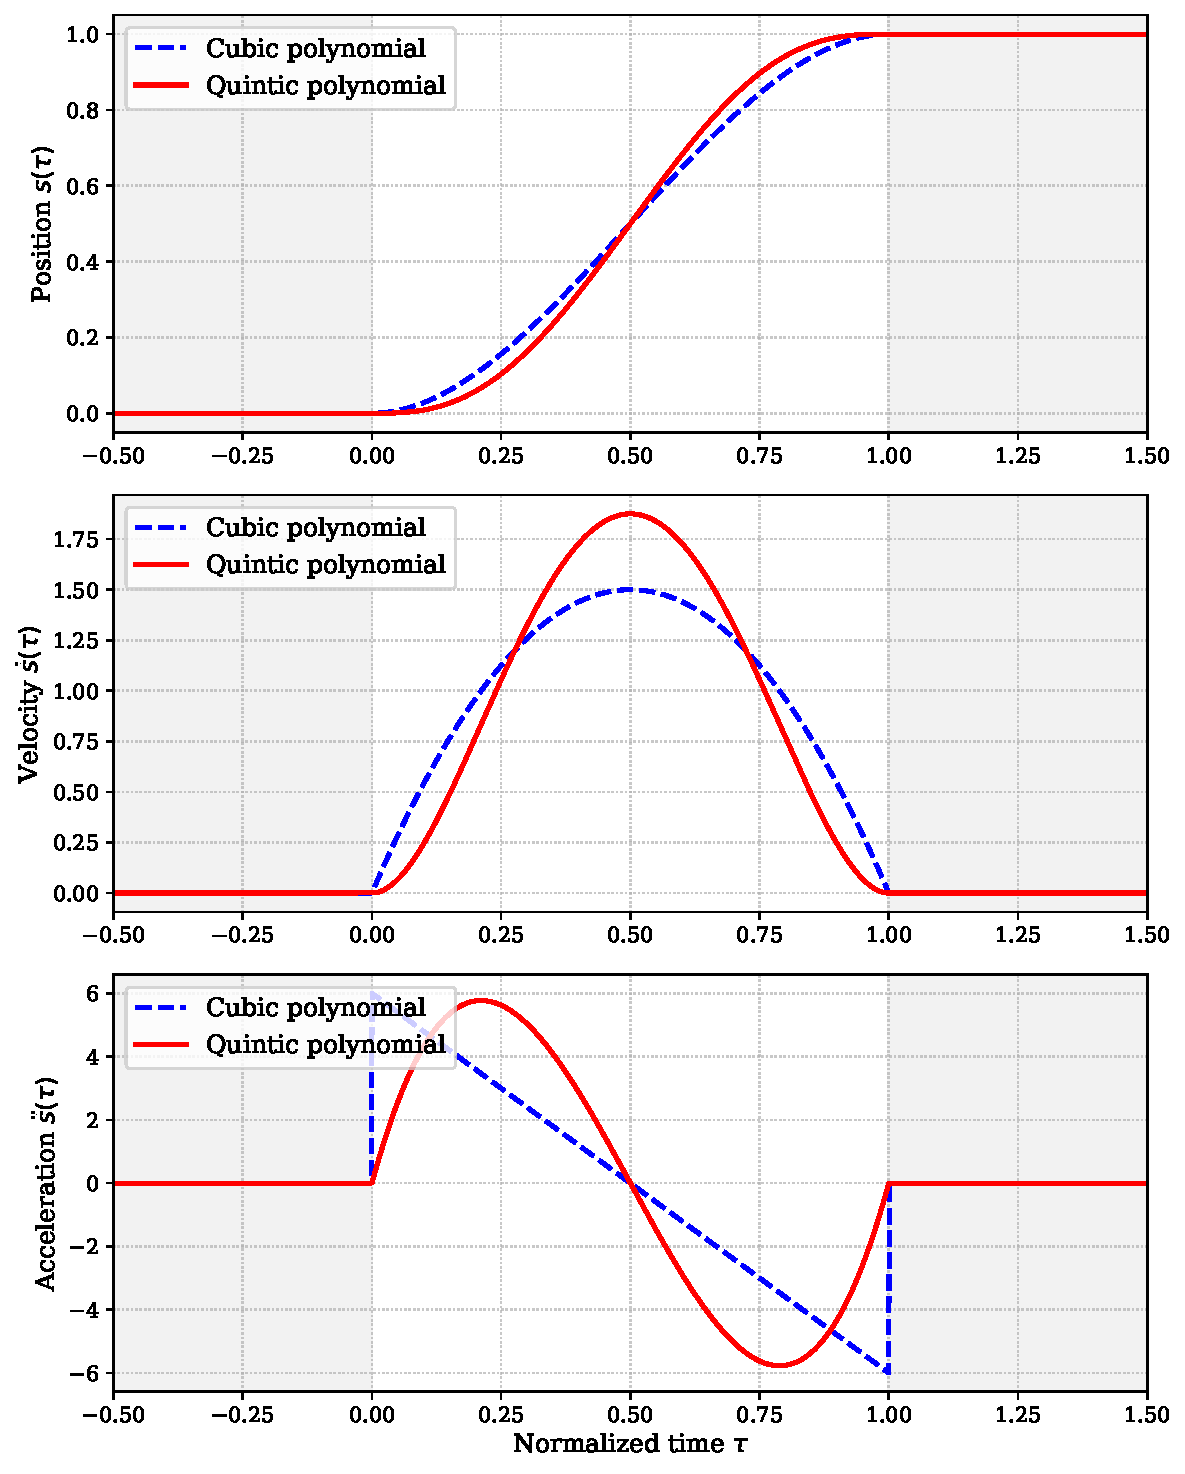
\includegraphics[width=0.8\textwidth]{gait_planner/cubic_vs_quintic.pdf}
    \caption{So sánh biên dạng động học giữa nội suy bậc 3 và bậc 5.}
    \label{fig:cubic_vs_quintic}
\end{figure}

Từ Hình~\ref{fig:cubic_vs_quintic}, có thể thấy rõ sự khác biệt ở biên dạng gia tốc. Đối với đa thức bậc 3, gia tốc tại các thời điểm chuyển pha ($\tau=0$ và $\tau=1$) có giá trị khác không ($\pm 6$). Sự thay đổi đột ngột gia tốc từ 0 lên giá trị này gây ra lực giật (jerk), dẫn đến rung lắc cơ khí và lực va đập tại các khớp của robot. Ngược lại, đối với đa thức bậc 5, gia tốc tại $\tau=0$ và $\tau=1$ hoàn toàn bằng không, tạo sự chuyển tiếp mượt mà về mặt động lực học. Quỹ đạo đạt độ trơn bậc hai ($C^2$), hoàn toàn phù hợp với yêu cầu chuyển động ổn định của robot bốn chân trong thực tế.

Do đó, tác giả sử dụng hoàn toàn nội suy đa thức bậc năm cho việc tạo quỹ đạo bước chân nhằm tăng cường sự ổn định và kéo dài tuổi thọ của hệ thống truyền động.

\subsection{Triển khai quỹ đạo chân dạng chữ D}

Trong hệ thống thực tế, quỹ đạo của mỗi chân robot được chia thành hai pha: pha vung chân (swing phase) và pha chống chân (stance phase), tạo thành đường đi dạng chữ D trong không gian Descartes.

\textbf{\textit{Pha vung (Swing Phase)}} 

Trong pha vung, chân di chuyển từ vị trí bắt đầu $\mathbf{p}_A$ (phía sau) đến vị trí kết thúc $\mathbf{p}_D$ (phía trước) trong $N_{sw}$ bước. Tọa độ ngang ($x$, $y$) được nội suy bằng hàm bước mượt bậc năm:

\begin{align}
\tau &= \frac{i}{N_{sw} - 1}, \quad i = 0, 1, \ldots, N_{sw}-1 \\
s &= 10\tau^3 - 15\tau^4 + 6\tau^5 \\
x_i &= x_A + s \cdot (x_D - x_A) \\
y_i &= y_A + s \cdot (y_D - y_A)
\end{align}

Đối với tọa độ theo phương $z$, thay vì sử dụng đa thức bậc năm thuần túy, quỹ đạo nâng chân được thiết kế theo đường cong parabol trên biến $s$:

\begin{equation}
z_i = z_{stance} + \Delta h \cdot 4\,s\,(1 - s)
\label{eq:z_parabolic}
\end{equation}

trong đó $z_{stance}$ là chiều cao pha chống chân và $\Delta h$ là độ cao nâng chân. Biểu thức $4\,s\,(1-s)$ tạo ra đường cong hình chuông đối xứng đạt cực đại $\Delta h$ tại $s = 0.5$ (giữa pha vung chân), đồng thời trả về $z_{stance}$ tại $s = 0$ và $s = 1$ (đầu và cuối pha vung chân). Nhờ kế thừa tính liên tục $C^2$ từ hàm $s(\tau)$, quỹ đạo $z$ cũng mượt mà tại các điểm chuyển pha.

\textbf{\textit{Pha chống chân (Stance Phase)}} 

Trong pha chống chân, chân duy trì tiếp xúc mặt đất tại $z_{stance}$ và di chuyển ngược từ $\mathbf{p}_D$ về $\mathbf{p}_A$ trong $N_{st}$ bước, cũng sử dụng hàm bước mượt bậc năm:

\begin{align}
\tau &= \frac{i}{N_{st} - 1}, \quad i = 0, 1, \ldots, N_{st}-1 \\
s &= 10\tau^3 - 15\tau^4 + 6\tau^5 \\
x_i &= x_D + s \cdot (x_A - x_D) \\
y_i &= y_D + s \cdot (y_A - y_D) \\
z_i &= z_{stance}
\end{align}

Tổng số điểm quỹ đạo cho một chu kỳ dáng đi đầy đủ là $N_{total} = N_{sw} + N_{st}$.

\begin{figure}[H]
    \centering
    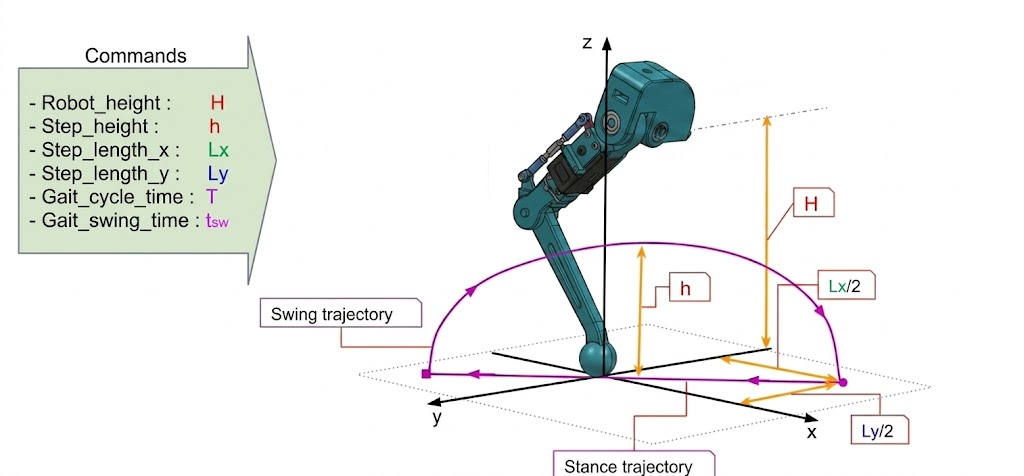
\includegraphics[width=0.8\textwidth]{gait_planner/gait_generator.png}
    \caption{Quỹ đạo chân 3D dạng chữ D (Pha vung Parabol và Pha chống đỡ đường thẳng)}
    \label{fig:gait_trajectory_3d}
\end{figure}

\subsection{Tham số quỹ đạo trong hệ thống thực tế}

Vị trí bắt đầu và kết thúc cho mỗi chân được tính theo:

\begin{align}
x_A &= x_{center} - \frac{L_{stride}}{2}, \quad x_D = x_{center} + \frac{L_{stride}}{2} \\
z_A &= z_D = z_{stance}
\end{align}

Hệ số chu kỳ nhiệm vụ (duty cycle) tổng quát được xác định là:

\begin{equation}
\beta = \frac{N_{st}}{N_{st} + N_{sw}}
\end{equation}

Dáng đi Trot yêu cầu giá trị $\beta > 0.5$, đảm bảo robot luôn có ít nhất hai chân tiếp xúc mặt đất tại mọi thời điểm để duy trì ổn định tĩnh trong suốt chu kỳ.

\subsection{Lập lịch pha dáng đi}

Dáng đi (gait) của robot bốn chân được xác định bởi mối quan hệ pha giữa các chân. Mỗi chân thực hiện cùng một quỹ đạo tuần hoàn, nhưng với độ lệch pha khác nhau. Pha dịch $\phi_i \in [0, 1)$ xác định vị trí tương đối của chân $i$ trong chu kỳ dáng đi tổng thể.

Trong triển khai thực tế, mỗi chân duy trì một chỉ số bước (waypoint index) $k_i$ trong mảng quỹ đạo tổng $N_{total} = N_{sw} + N_{st}$ điểm. Pha dịch được áp dụng bằng cách khởi tạo chỉ số bắt đầu của mỗi chân:

\begin{equation}
    k_{i,0} = \lfloor \phi_i \cdot N_{total} \rfloor
\end{equation}

Bảng~\ref{tab:gait_phases} trình bày các cấu hình pha dịch cho ba dáng đi phổ biến nhất.

\begin{table}[H]
\centering
\caption{Cấu hình pha dịch cho các dáng đi}
\label{tab:gait_phases}
\renewcommand{\arraystretch}{1.3}
\begin{tabular}{|l|c|c|c|c|c|}
\hline
\textbf{Dáng đi} & $\phi_{LF}$ & $\phi_{RF}$ & $\phi_{LB}$ & $\phi_{RB}$ & \textbf{Đặc điểm} \\ \hline
Trot & 0 & 0,5 & 0,5 & 0 & Hai chân chéo đồng pha \\ \hline
Walk & 0 & 0,5 & 0,75 & 0,25 & Tuần tự từng chân \\ \hline
Pace & 0 & 0,5 & 0 & 0,5 & Hai chân cùng bên đồng pha \\ \hline
\end{tabular}
\end{table}

\textbf{\textit{Dáng đi Trot}} 

($\phi = [0, 0.5, 0.5, 0]$) là cấu hình dáng đi phổ biến nhất. Hai chân chéo (LF--RB và RF--LB) hoạt động đồng pha, tạo ra hai nhóm chân xen kẽ. Tại mọi thời điểm, ít nhất hai chân thuộc cùng nhóm đang ở pha chống chân, duy trì ổn định tĩnh.

\textbf{\textit{Phân tích thời gian một chu kỳ}} 

Tổng thời gian của một chu kỳ dáng đi đầy đủ phụ thuộc vào số lượng khung hình (frame) của các pha và chu kỳ bộ định thời (timer period) $\Delta T$:

\begin{equation}
    T_{cycle} = (N_{sw} + N_{st}) \times \Delta T
\end{equation}

Tần số bước chân được tính theo chu kỳ:

\begin{equation}
    f_{step} = \frac{1}{T_{cycle}}
\end{equation}

Từ đó, tốc độ di chuyển tiến về phía trước theo lý thuyết là tích của chiều dài bước và tần số bước:

\begin{equation}
    v_{forward} = L_{stride} \times f_{step}
\end{equation}

Tốc độ này có thể được điều chỉnh trực tiếp thông qua việc thay đổi sải bước $L_{stride}$ hoặc thay đổi thời gian pha chống chân $N_{st}$.



\section{Thiết kế bộ điều khiển}

Để robot có thể duy trì thăng bằng và phản hồi chính xác với các nhiễu loạn ngoại lai (ví dụ: bề mặt địa hình gồ ghề), một hệ thống điều khiển vòng kín tự động dựa trên thuật toán PID được thiết kế. Cấu trúc tổng thể của hệ thống tự cân bằng này được trình bày chi tiết trong Hình~\ref{fig:applied_pid_simulink}.

Hệ thống hoạt động dựa trên cơ chế phản hồi trạng thái động học thông qua các khâu xử lý liên tiếp. Bắt đầu từ khâu đo lường và tạo sai số, cảm biến IMU (BNO055) liên tục đo lường góc nghiêng thực tế của thân robot (True Roll/Pitch). Các giá trị này được so sánh với góc tham chiếu lý thuyết (thường đặt $\phi_{ref}=0, \theta_{ref}=0$) thông qua các bộ cộng để tạo ra tín hiệu sai số $e_\phi$ và $e_\theta$. Tiếp đó, sai số được đưa vào bộ điều khiển PID (tích hợp khâu chống vọt lố Anti-windup và lọc thông thấp LPF), với đầu ra của khối này là các tín hiệu bù cân bằng (Compensation Signals). Tại khối chuyển mạch chế độ (Mode Switch), tùy thuộc vào trạng thái hiện tại của robot, hệ thống sẽ rẽ nhánh luồng tín hiệu bù. Đối với chế độ di chuyển (GAIT Mode), tín hiệu bù được gửi tới khối Quy hoạch quỹ đạo và Động học nghịch (Trajectory Planning \& Inverse Kinematics) để tính toán bù trừ trực tiếp vào tọa độ không gian làm việc của bàn chân. Ngược lại, đối với chế độ đứng yên (HOME Mode), tín hiệu bù được gửi tới khối Bù góc khớp trực tiếp (Direct Joint Angle Compensator) để tinh chỉnh không gian khớp. Cuối cùng, trong khâu thực thi, các góc khớp mục tiêu ($\theta_i$) được truyền xuống cơ cấu chấp hành (Bus Servo ST3215) để tác động lực lên đối tượng vật lý (Quadruped Robot Plant), từ đó tạo ra các chuyển động triệt tiêu nhiễu loạn và giúp thân robot lấy lại tư thế ngang bằng.

\begin{figure}[H]
    \centering
    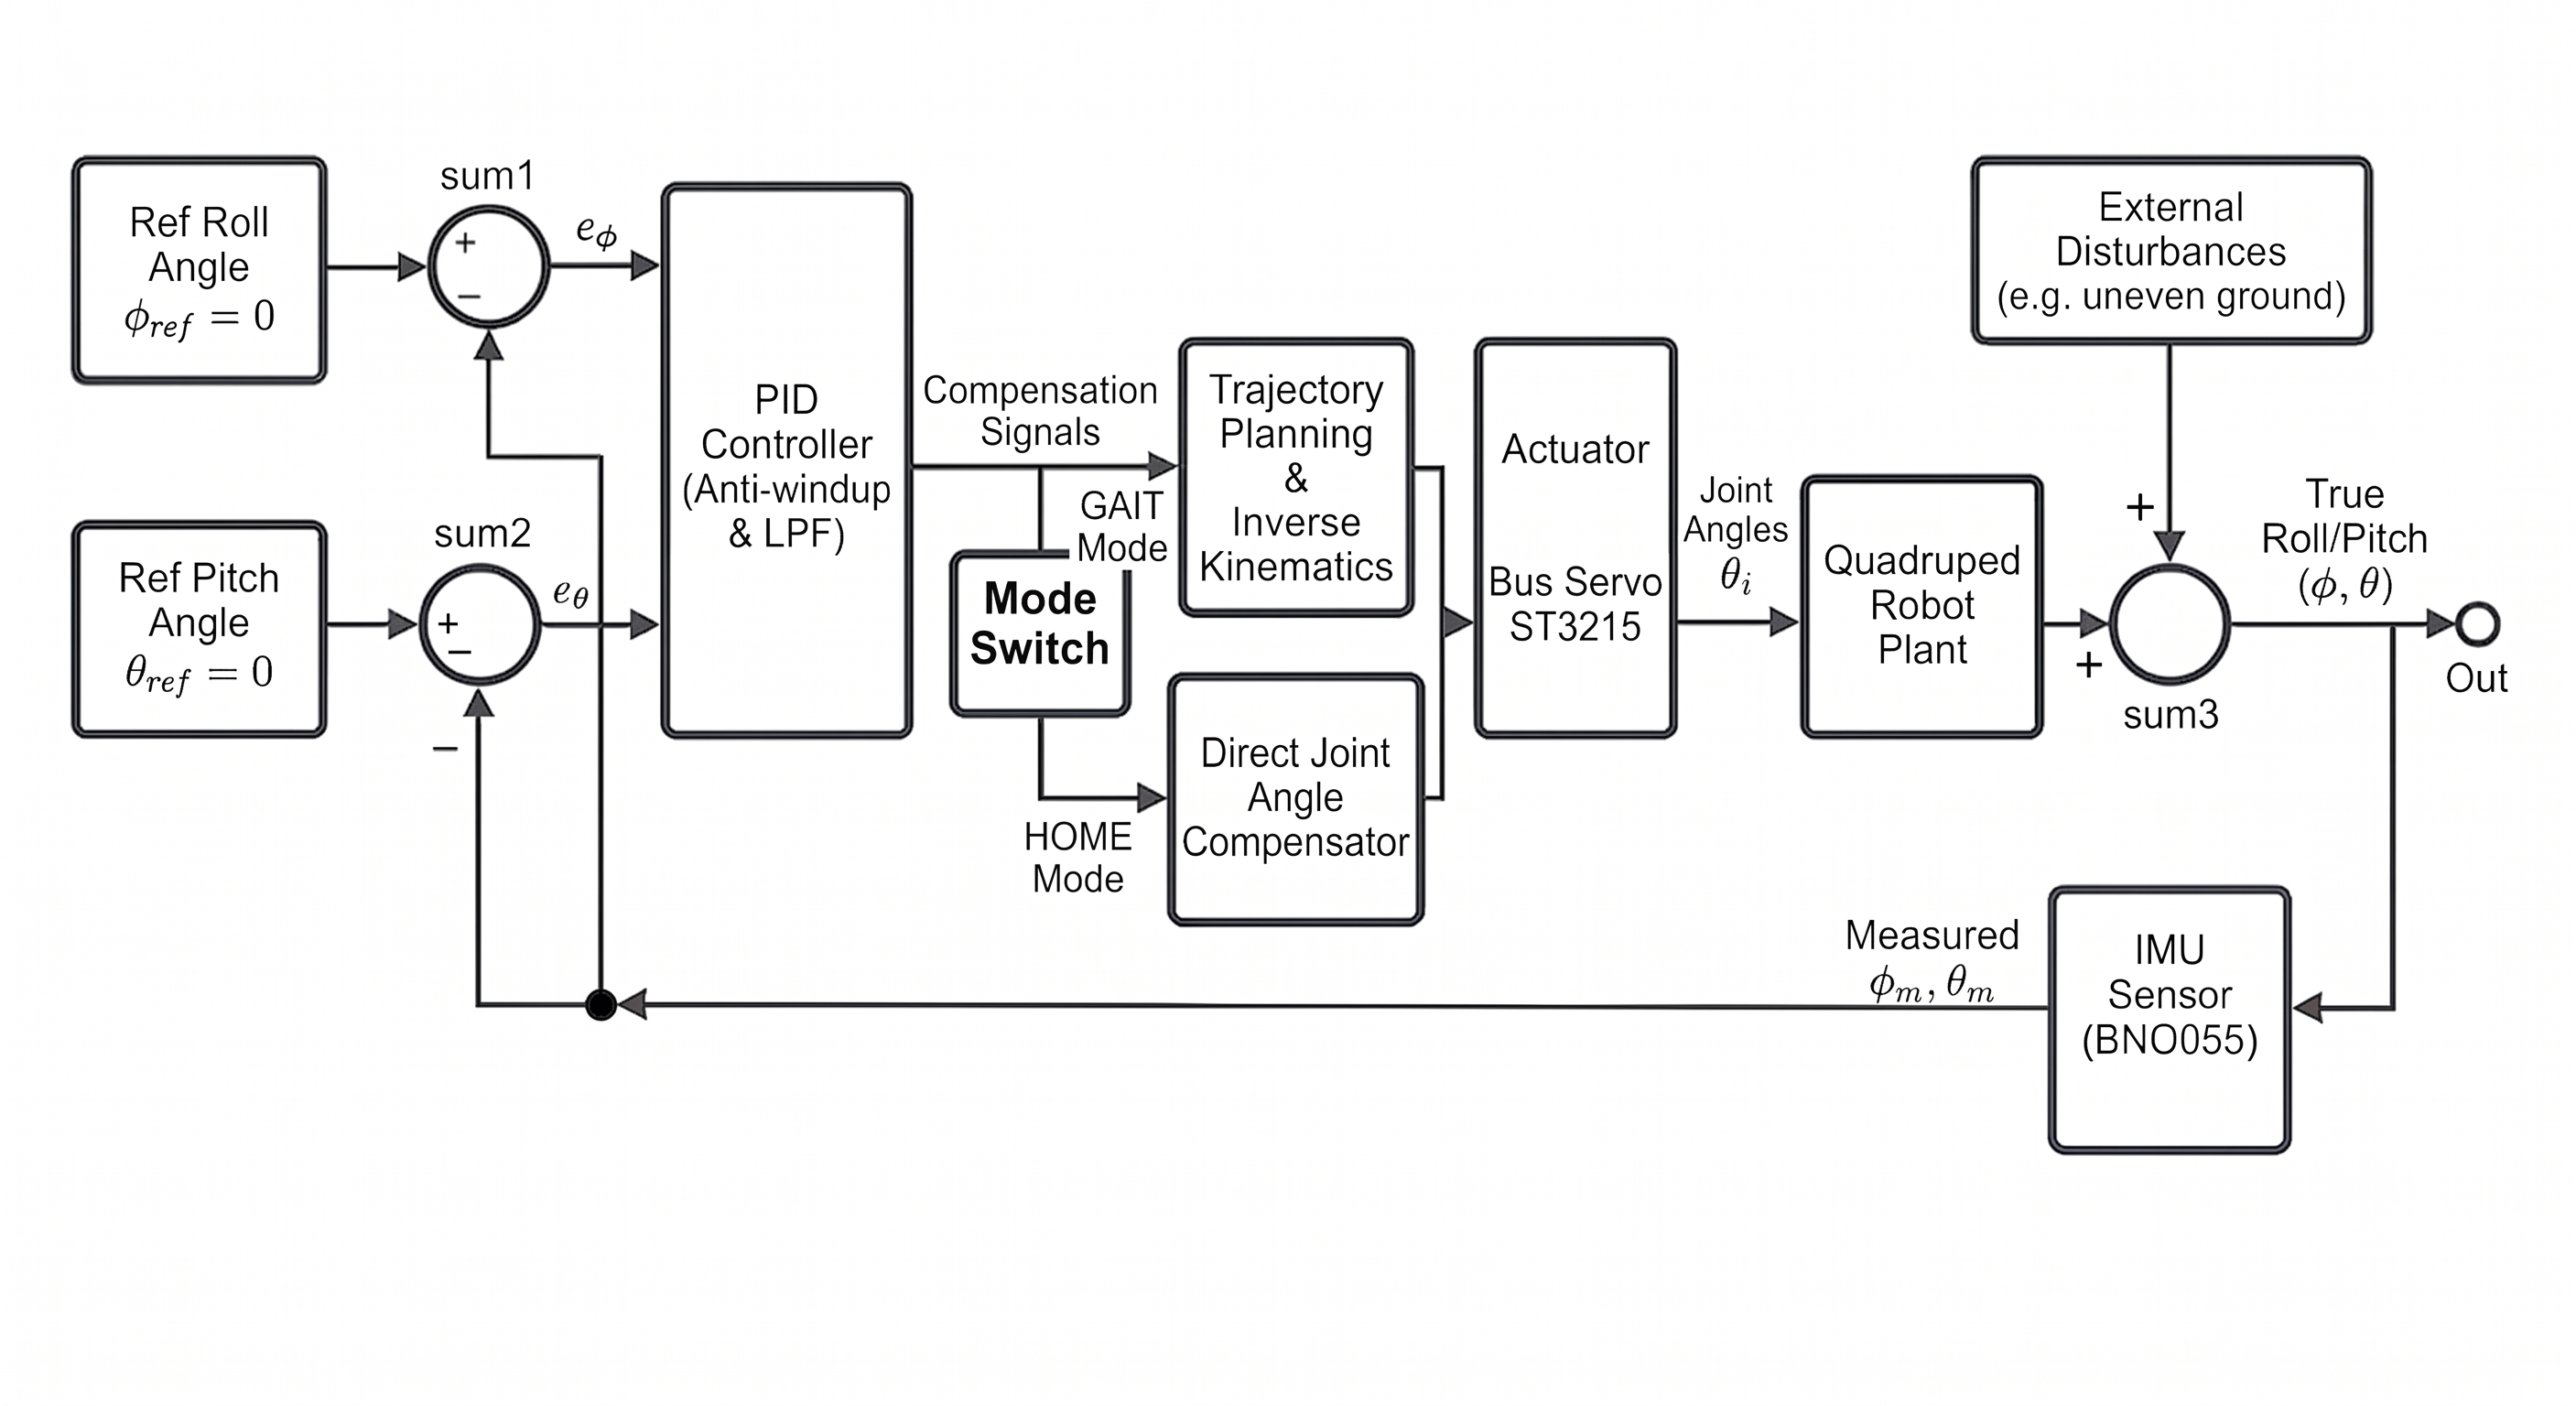
\includegraphics[width=\textwidth]{img_matlab/fig-PID.png}
    \caption{Sơ đồ khối bộ điều khiển tự cân bằng của robot bốn chân.}
    \label{fig:applied_pid_simulink}
\end{figure}



\subsection{Kiến trúc điều khiển chi tiết}

Hệ thống điều khiển tổng thể của robot hoạt động với tần số vòng lặp 333~Hz ($\Delta T = 3$~ms), được thiết kế theo cấu trúc phân cấp chặt chẽ (Hình~\ref{fig:overall_architecture_locomotion}). Hệ thống tiếp nhận các lệnh cấp cao từ người dùng (User Commands) thông qua một máy trạng thái trung tâm (Command Manager) và điều phối luồng dữ liệu xuống các thành phần xử lý cốt lõi, bao gồm Bộ quy hoạch chuyển động (Locomotion Planner) và Bộ điều khiển cân bằng (Balance Controller).

\begin{figure}[H]
    \centering
    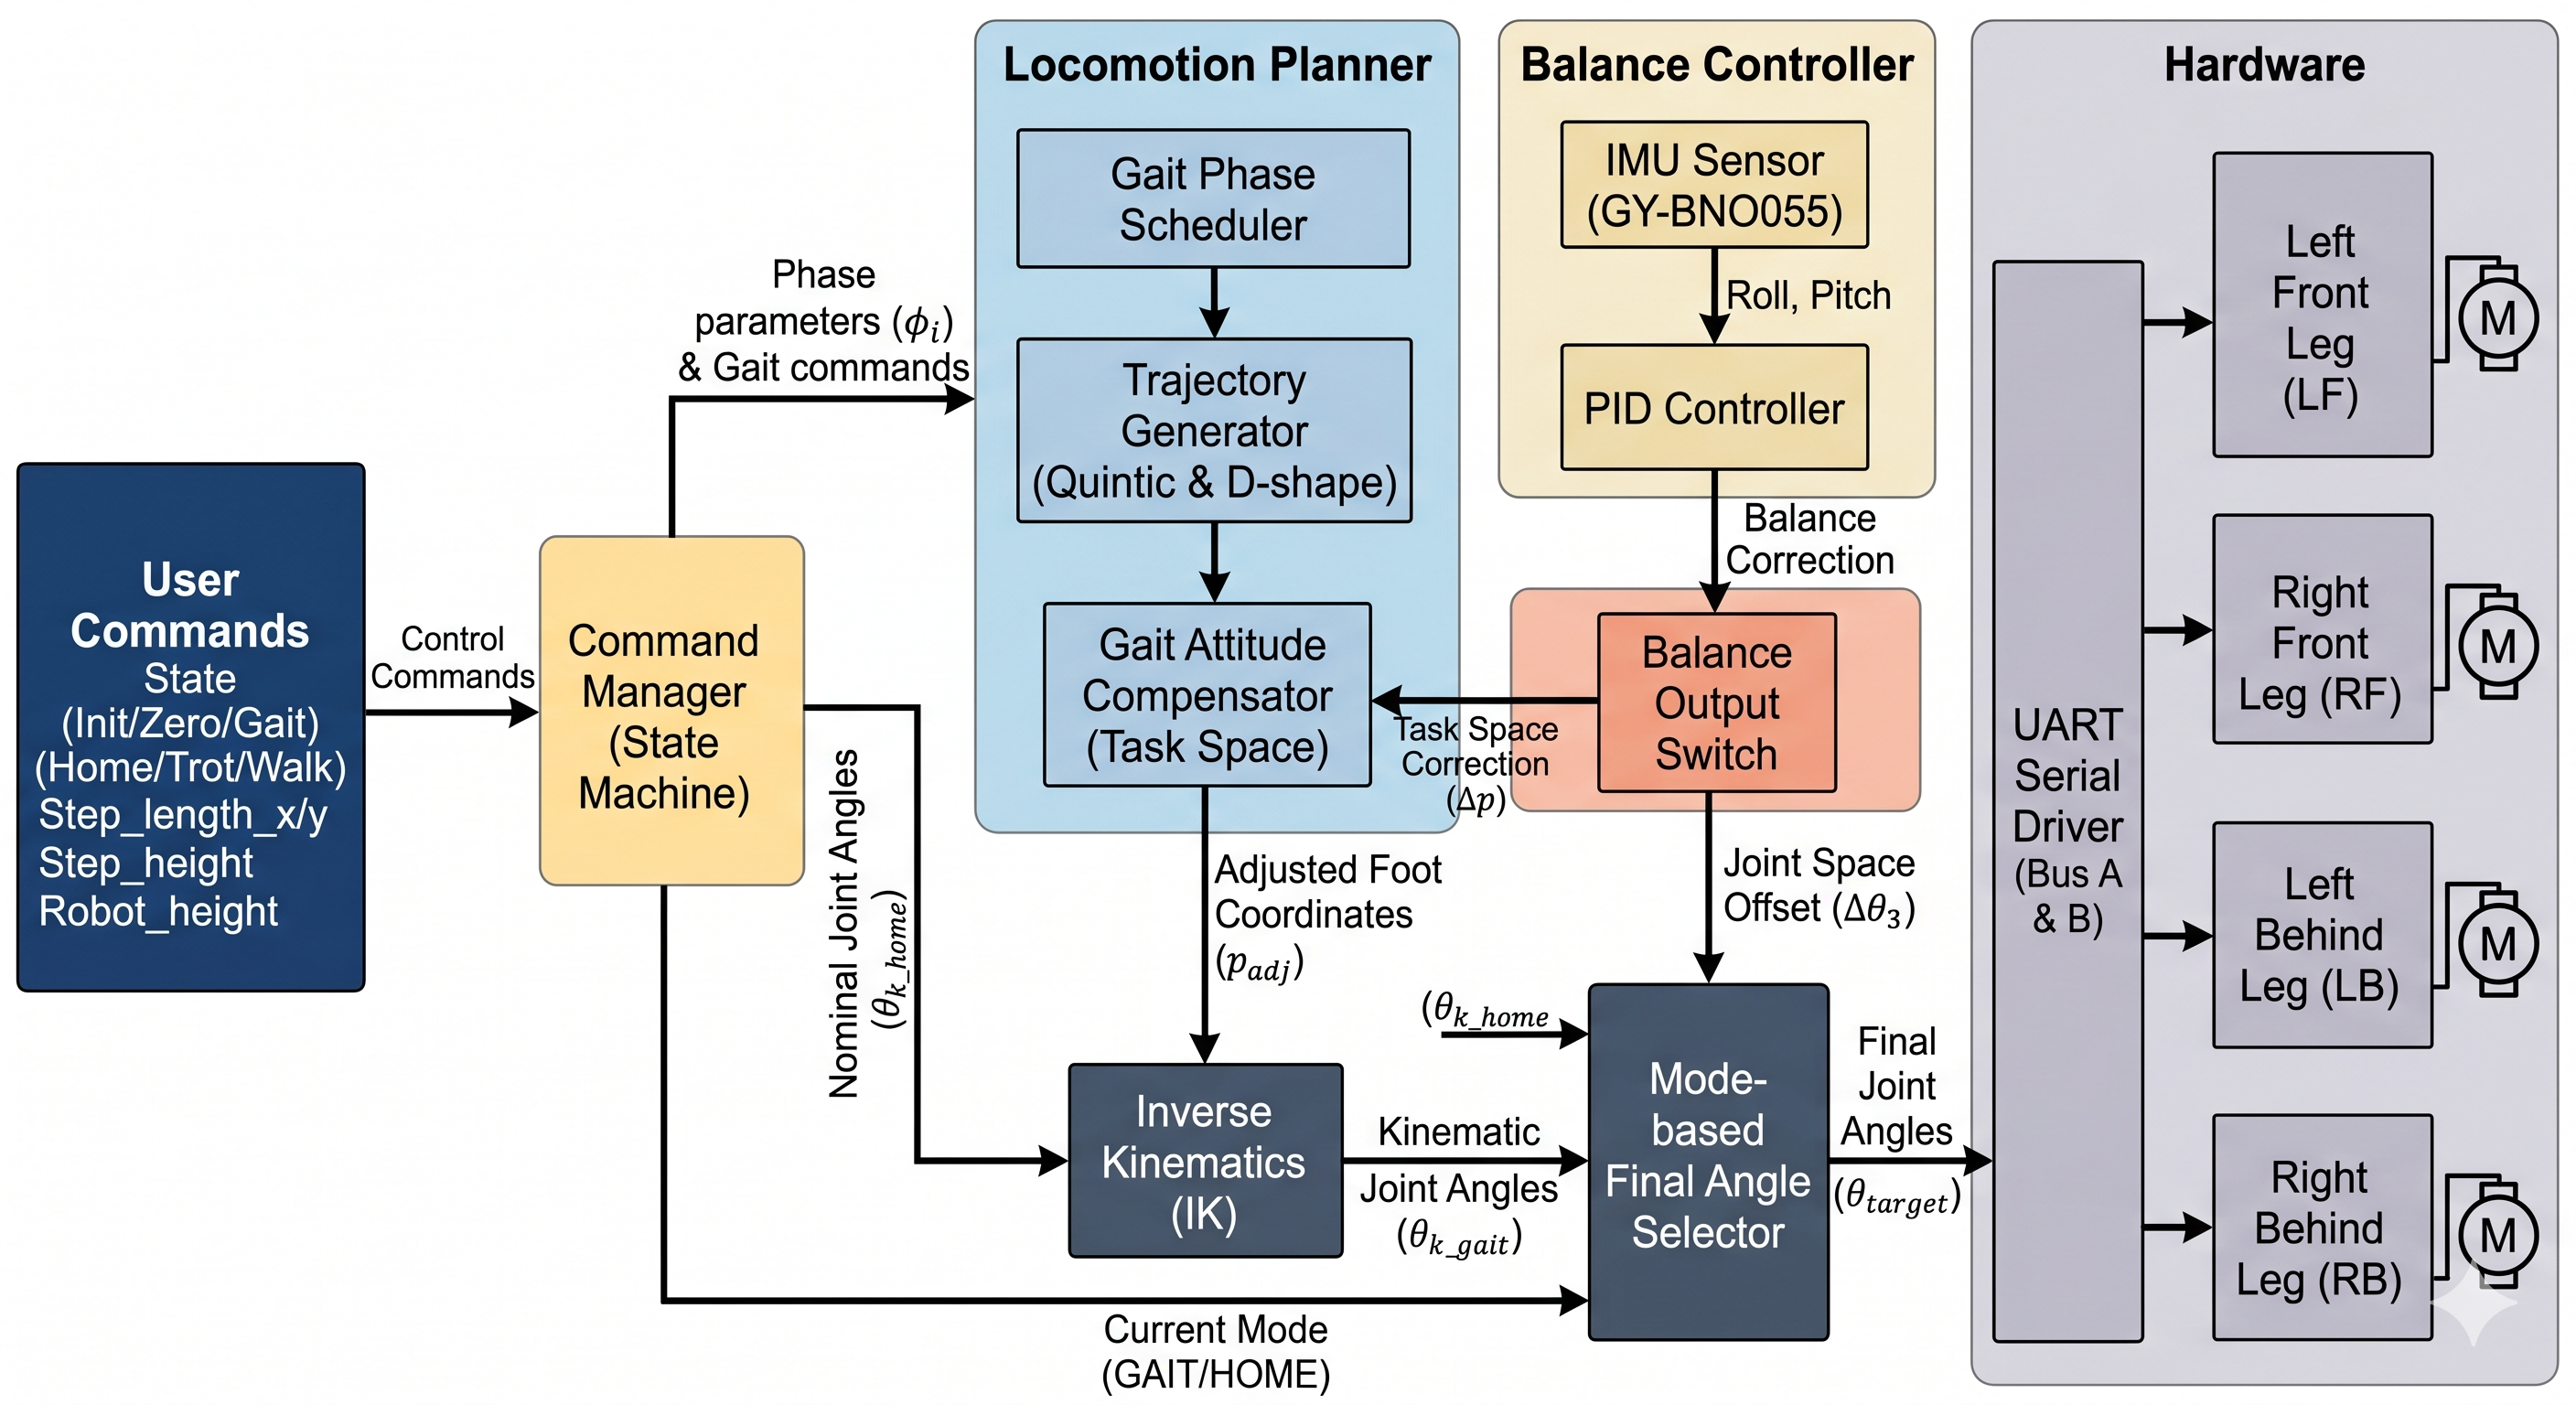
\includegraphics[width=\textwidth]{architecture/locomotion_balance_controller.png}
    \caption{Tổng quan kiến trúc điều khiển hệ thống robot bốn chân tích hợp bộ chuyển mạch chế độ tĩnh/động.}
    \label{fig:overall_architecture_locomotion}
\end{figure}

Đặc điểm nổi bật của kiến trúc này là khả năng phân chia luồng xử lý độc lập cho trạng thái di chuyển (Gait Mode) và trạng thái đứng yên (Home Mode), kết hợp với cơ chế phản hồi thăng bằng linh hoạt thông qua ba thành phần chính. Thành phần thứ nhất là Bộ quy hoạch chuyển động (Locomotion Planner), đóng vai trò là module chịu trách nhiệm tạo hình quỹ đạo chân khi robot di chuyển; module này bao gồm Bộ lập lịch pha (Gait Phase Scheduler) để đồng bộ thời gian các chân, kết hợp với Bộ tạo quỹ đạo (Trajectory Generator) để sinh ra tọa độ bước chân dạng đa thức Quintic và D-shape. Thành phần thứ hai là Khối bù tư thế không gian làm việc (Gait Attitude Compensator) nằm trong cụm Planner; khối này nhận tọa độ nguyên bản và cộng bù trực tiếp với tín hiệu chỉnh sửa $\Delta p$ từ bộ thăng bằng, sinh ra tọa độ chân hiệu chỉnh $p_{adj}$ trước khi đưa vào khâu giải động học nghịch (IK). Thành phần thứ ba là Bộ điều khiển cân bằng (Balance Controller) hoạt động hoàn toàn độc lập, sử dụng dữ liệu góc Roll/Pitch từ IMU làm phản hồi cho bộ PID để liên tục tính toán lượng bù chống lại ngoại lực gây lật thân.

Sự linh hoạt của hệ thống nằm ở công tắc chuyển mạch điều chỉnh cân bằng (\textit{Balance Output Switch}) và bộ chọn góc khớp cuối cùng (\textit{Mode-based Final Angle Selector}). Tùy thuộc vào chế độ hoạt động hiện tại, tín hiệu bù cân bằng sẽ được định tuyến theo hai phương thức hoàn toàn khác biệt. Trong chế độ tĩnh (HOME), hệ thống áp dụng cơ chế bù trong không gian khớp (Joint Space); khi robot đứng im, quỹ đạo làm việc bị khóa, tín hiệu bù từ PID được chuyển mạch thành độ dịch góc khớp ($\Delta\theta_3$). Độ dịch này sau đó được bộ Final Angle Selector cộng trực tiếp vào góc khớp gối danh định $\theta_{k\_home}$ để gửi ngay xuống phần cứng (UART Serial Driver). Việc bỏ qua hoàn toàn cụm tính toán IK giúp phản ứng cân bằng đạt độ trễ tối thiểu, khử nhiễu ngoại lực tức thời. Ngược lại, trong chế độ động (GAIT), hệ thống áp dụng cơ chế bù trong không gian làm việc (Task Space); khi robot đang bước đi, việc bảo toàn quỹ đạo chân 3D là yếu tố bắt buộc. Tín hiệu bù từ PID lúc này được chuyển đổi thành độ dời tọa độ ($\Delta p$) và đưa ngược vào bộ Gait Attitude Compensator. Bằng cách bù vào đầu vào của khối IK thay vì cộng trực tiếp vào góc khớp, robot có thể vừa giữ thăng bằng thân vừa bảo toàn chính xác hình dáng biên độ bước đi, tránh tình trạng trượt chân (slippage) tại các điểm đặt.

\subsection{Cơ chế áp dụng tín hiệu điều chỉnh tư thế}
Việc điều chỉnh tư thế được thực hiện theo thời gian thực thông qua quá trình đo đạc góc nghiêng từ cảm biến IMU. Đầu ra của các bộ điều khiển PID là các tín hiệu bù hiệu chỉnh $u_{roll}$ và $u_{pitch}$. Sự khác biệt cốt lõi giữa hai chế độ hoạt động nằm ở \textit{không gian} mà tín hiệu hiệu chỉnh được ánh xạ.

\subsubsection*{Áp dụng hiệu chỉnh trong không gian khớp ở chế độ tĩnh}
Khi robot ở trạng thái tĩnh (chế độ HOME), tín hiệu $u_{roll}, u_{pitch}$ từ bộ điều khiển PID được phân bổ thành giá trị độ lệch (offset) cho từng chân, với giới hạn bão hòa $|\Delta\theta_3| \leq \theta_{sat}$:
\begin{equation}
\begin{cases} 
\Delta\theta_{3,LF} = \mathrm{sat}\big(- (K_{home} u_{roll} - K_{home} u_{pitch}),\; \theta_{sat}\big) \\
\Delta\theta_{3,LB} = \mathrm{sat}\big(- (K_{home} u_{roll} + K_{home} u_{pitch}),\; \theta_{sat}\big) \\
\Delta\theta_{3,RF} = \mathrm{sat}\big(- (K_{home} u_{roll} + K_{home} u_{pitch}),\; \theta_{sat}\big) \\
\Delta\theta_{3,RB} = \mathrm{sat}\big(- (K_{home} u_{roll} - K_{home} u_{pitch}),\; \theta_{sat}\big) 
\end{cases}
\end{equation}
Lượng bù này được cộng trực tiếp làm giá trị hiệu chỉnh cho góc khớp gối ($\theta_3$). Do cấu trúc động học chuỗi hở, việc thay đổi trực tiếp góc khớp gối sẽ làm thay đổi vị trí bàn chân tương ứng. Động thái này tạo ra các phản lực từ mặt đất, giúp thân robot lấy lại trạng thái cân bằng tức thời mà không yêu cầu hệ thống phải tính toán qua khối động học nghịch (IK), qua đó giảm thiểu tối đa độ trễ điều khiển.

\subsubsection*{Áp dụng hiệu chỉnh trong không gian làm việc ở chế độ động}
Khi robot đang trong chu trình di chuyển (chế độ GAIT), biên dạng quỹ đạo bước chân bắt buộc phải được bảo toàn nghiêm ngặt để tránh hiện tượng trượt (slippage) và mất ổn định chu kỳ. Do đó, ma trận xoay nghịch đảo $R = R_y(u_{pitch}) R_x(u_{roll})$ được tính toán dựa trên lượng bù từ bộ điều khiển PID. Ma trận này sau đó được nhân với vectơ vị trí chân nguyên bản $\mathbf{p}_{raw}$ sinh ra từ bộ tạo quỹ đạo. Một cơ chế chọn lọc được áp dụng nhằm chỉ cập nhật duy nhất tọa độ cao độ trục Z của bàn chân, trong khi cố định hoàn toàn các giá trị tham chiếu trên trục X và Y:
\begin{equation}
\mathbf{p}_{adj} = R \cdot \mathbf{p}_{raw}, \quad \text{với} \quad x_{adj} = x_{raw}, \quad y_{adj} = y_{raw}
\end{equation}

Nguyên lý giữ nguyên sự biến thiên trên mặt phẳng XY đóng vai trò then chốt trong việc bảo toàn chiều dài sải bước (stride length) của robot. Tọa độ Đề-các hiệu chỉnh $[x_{adj}, y_{adj}, z_{adj}]$ sau đó mới được cấp vào bộ giải động học nghịch (IK) để suy ra góc quay mục tiêu cho các khớp. Quá trình biến đổi không gian này được minh họa trực quan trong Hình \ref{fig29}.

\begin{figure}[H]
    \centering
    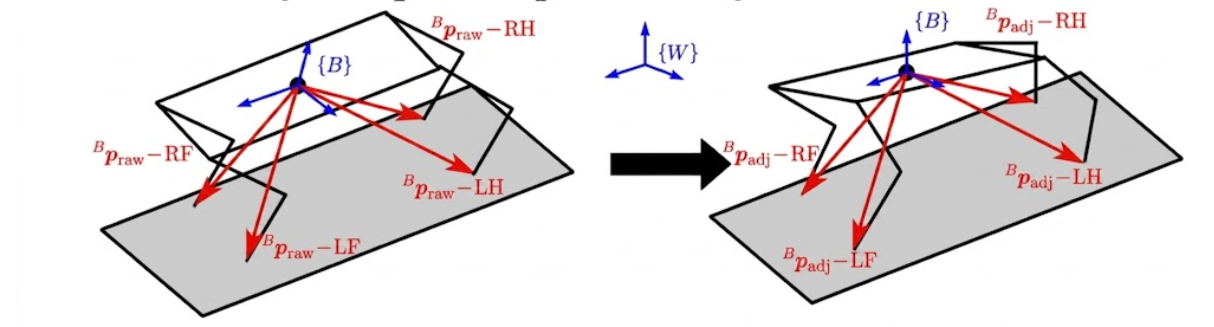
\includegraphics[width=0.9\textwidth]{kinematics/attitude_adjustment.png}
    \caption{Minh họa quá trình điều chỉnh tư thế thân robot: từ $\mathbf{p}_{raw}$ (trước bù) sang $\mathbf{p}_{adj}$ (sau bù), chỉ thay đổi trục $Z$, giữ nguyên trục $X$ và $Y$.}
    \label{fig29}
\end{figure}

\subsection{Thuật toán điều khiển PID và các khâu bảo vệ}
Trong cả hai chế độ động và tĩnh, thuật toán cốt lõi đảm nhiệm triệt tiêu sai lệch tư thế là bộ điều khiển PID kinh điển, được phân tách tính toán độc lập cho trục Roll và trục Pitch. Đầu vào của khối là sai số $e(t) = 0 - \theta_{meas}(t)$, trong đó $\theta_{meas}$ là giá trị góc nghiêng đo được từ IMU sau khi đã đi qua bộ lọc trung bình trượt hàm mũ (EMA) nhằm khử nhiễu cơ học tần số cao.

Luật điều khiển PID được triển khai dưới dạng phương trình sai phân rời rạc như sau:
\begin{equation}
    u_{PID}(k) = K_P e(k) + K_I \sum_{i=0}^{k} e(i) \Delta T + K_D \frac{e(k) - e(k-1)}{\Delta T}
\end{equation}

Nhằm đáp ứng yêu cầu an toàn tuyệt đối cho phần cứng robot khi vận hành thực tế, tín hiệu đầu ra của bộ PID buộc phải đi qua các lớp bảo vệ thiết yếu trước khi được phát lệnh tới cơ cấu chấp hành. Lớp bảo vệ đầu tiên là khâu triệt vùng chết (Deadband), chủ động bỏ qua các vi sai quá nhỏ dao động quanh vị trí cân bằng ($0$ rad); kỹ thuật này triệt tiêu hiện tượng chattering (động cơ rung lắc liên tục), qua đó giảm hao mòn cơ khí và tỏa nhiệt không cần thiết. Lớp bảo vệ thứ hai bao gồm bão hòa tín hiệu (Saturation) và lọc thông thấp (LPF); lệnh điều khiển $u_{PID}$ được giới hạn biên độ trong khoảng an toàn $[-u_{max}, u_{max}]$ để ngăn chặn các xung bù vượt quá khả năng chịu tải của cơ hệ, sau đó tín hiệu được làm mượt qua bộ lọc thông thấp (Low-Pass Filter) để các khớp chuyển động êm ái, hạn chế tối đa các lực giật (jerk) cục bộ. Lớp bảo vệ cuối cùng là cơ chế chống tích lũy (Anti-windup); khi cơ cấu chấp hành hoặc tín hiệu đầu ra chạm ngưỡng bão hòa vật lý, cơ chế anti-windup sẽ tự động tạm dừng hoặc suy giảm thành phần tích phân $I$. Điều này chặn đứng sự tích lũy sai số ảo dư thừa, giúp hệ thống phục hồi nhanh chóng và không bị vọt lố (overshoot) khi các nhiễu loạn ngoại lực kết thúc.

Việc phân bổ linh hoạt chiến lược bù theo không gian làm việc tương ứng với trạng thái động học, kết hợp cùng các cơ chế bảo vệ tín hiệu nhiều lớp, là cơ sở khoa học then chốt giúp hệ thống điều khiển vận hành ổn định và bám sát lý thuyết động lực học.

% !TeX root = ../thesis.tex
\chapter{THIẾT KẾ VÀ THỰC HIỆN PHẦN CỨNG}

% !TeX root = ../thesis.tex



\section{Phân tích kết cấu robot}

\subsection{Thiết kế thân}
Thân của robot bốn chân là bộ phận trung tâm của toàn bộ kết cấu robot. Bốn chân được liên kết với nhau thông qua thân, do đó thiết kế thân cần đáp ứng các yêu cầu sau: 

Thứ nhất, phải có độ bền đủ lớn để đảm bảo không xảy ra biến dạng, nứt gãy,… trong quá trình robot di chuyển. 

Thứ hai, để đạt được khả năng di chuyển linh hoạt và hiệu quả năng lượng cao, thân robot cần được thiết kế nhẹ nhất có thể. 

Ngoài ra, bên trong thân robot phải có không gian đủ lớn để lắp đặt các servo, pin, bo mạch điều khiển, module chuyển đổi điện áp và các linh kiện khác. 

Cuối cùng, 12 servo được lắp tại các khớp chân cần có thiết kế riêng cho đường đi dây và vị trí lắp đặt, vì chúng luôn chuyển động tương đối so với thân robot khi robot đi bộ hoặc chạy chậm. 

Dựa trên các yêu cầu trên, thân robot được thiết kế theo dạng liền khối, nhằm ngăn ngừa biến dạng hoặc gãy vỡ. 

Bốn góc của thân được thiết kế để kết nối với cụm khớp hông, đảm bảo không xảy ra giao thoa cơ khí khi khớp hông quay theo bất kỳ hướng nào. 

Ngoài ra, tại những vị trí có khả năng chịu tải thấp, cấu trúc được khoét rỗng hợp lý để giảm khối lượng. Mô hình 3D của cấu trúc thân robot bốn chân được thể hiện ở Hình \ref{fig12-c} bên dưới.

\begin{figure}[H]
    \centering
    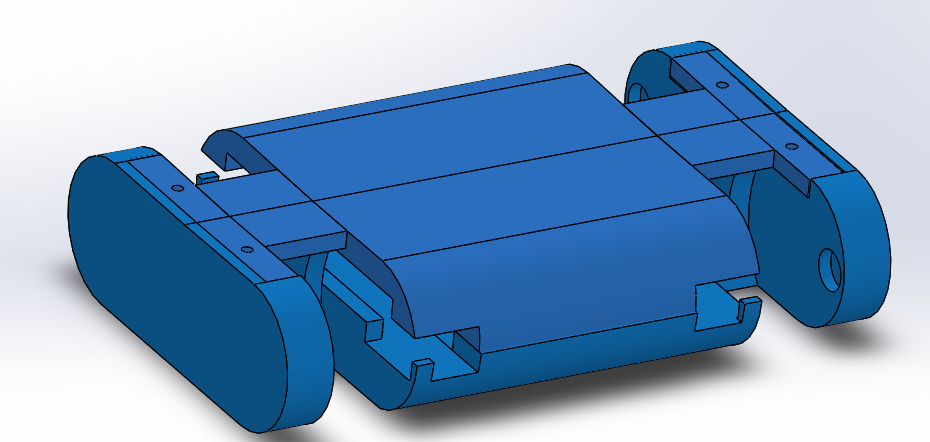
\includegraphics[width=0.6\textwidth]{hardware/body_part_c.png}
    \caption{Thiết kế thân liền khối nhằm đạt độ bền cao và khối lượng nhẹ.}
    \label{fig12-c}
\end{figure}

\begin{figure}[H]
    \centering
    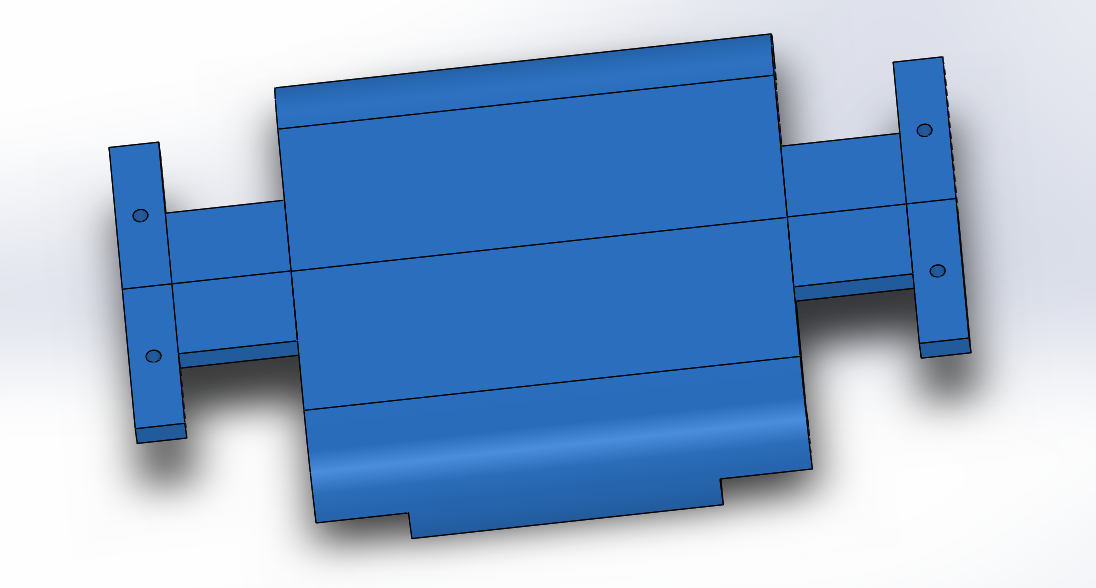
\includegraphics[width=0.6\textwidth]{hardware/body_part_b.png}
    \caption{Nắp thân.}
    \label{fig12-b}
\end{figure}

\begin{figure}[H]
    \centering
    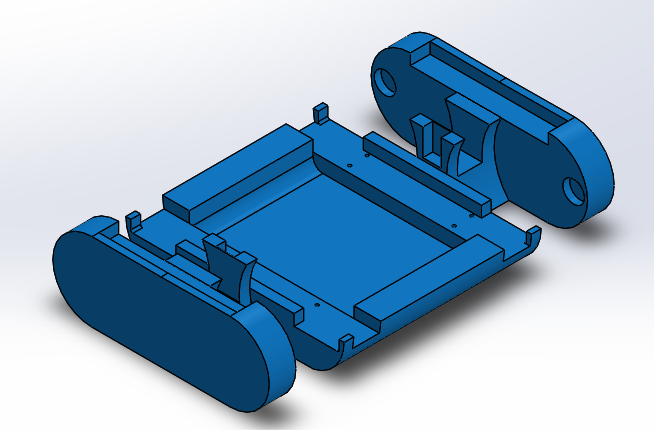
\includegraphics[width=0.6\textwidth]{hardware/body_part_a.png}
    \caption{Thiết kế thân.}
    \label{fig12-a}
\end{figure}


\subsection{Thiết kế khớp hông}

Khớp hông của robot bốn chân được thiết kế để tạo ra hai bậc tự do, một cho chuyển động roll và một cho chuyển động pitch. Mỗi chuyển động được truyền động bởi một servo.

Do servo được sử dụng trong thiết kế là loại servo một trục, các ổ bi mặt bích 626zz được sử dụng ở phía đối diện trục servo nhằm giảm lực hướng kính tác dụng lên trục. Đầu trục và khớp hông được tích hợp trong quá trình chế tạo, điều này giúp thuận tiện cho việc lắp đặt và giảm sai số lắp ráp.

Ngoài ra, servo điều khiển chuyển động vung trước (tức là chuyển động pitch) của khớp hông được lắp bên trong giá đỡ khớp hông để tiết kiệm không gian. Mô hình 3D của cụm khớp hông được thể hiện trong Hình \ref{fig13}.

\begin{figure}[H]
    \centering
    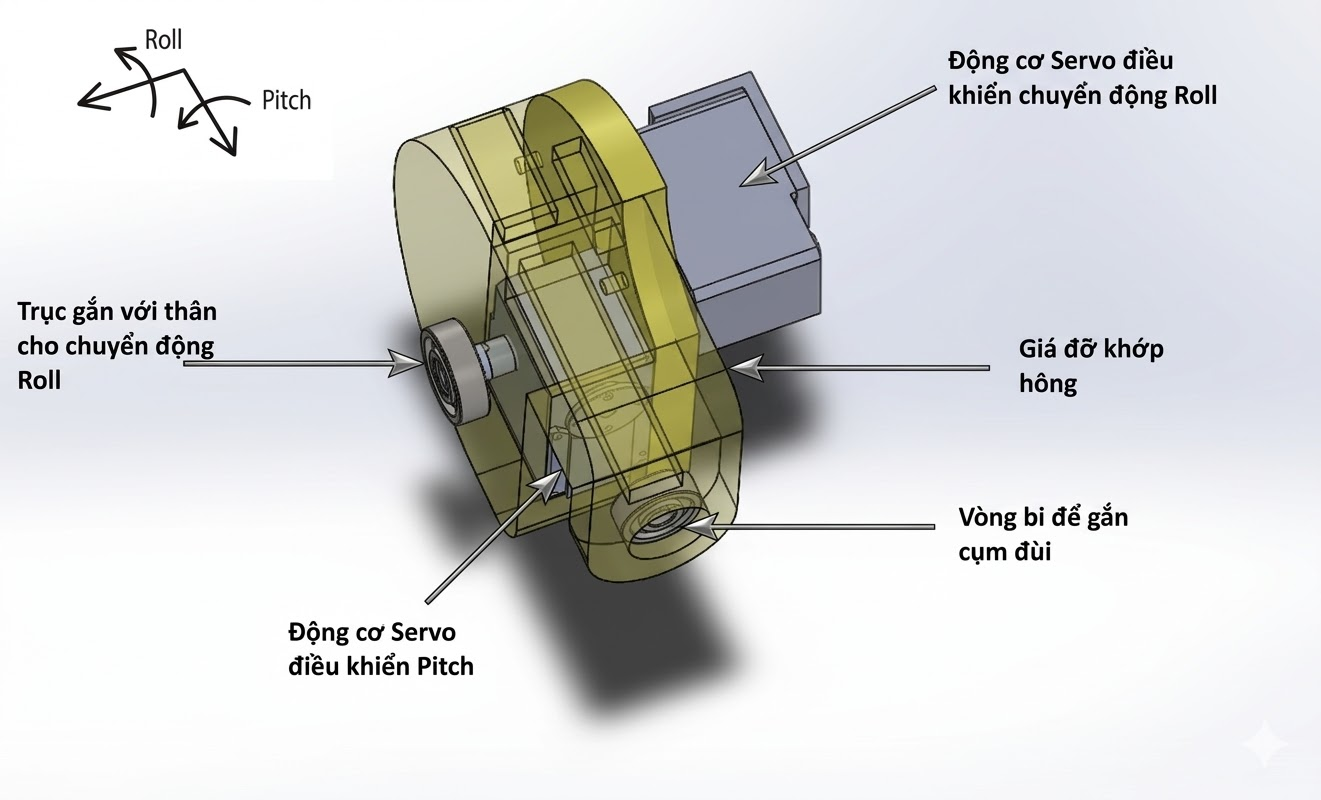
\includegraphics[width=0.6\textwidth]{hardware/hip_joint_assembly.jpg }
    \caption{Cụm khớp hông cho chuyển động vung ngang và vung dọc.}
    \label{fig13}
\end{figure}

\subsection{Thiết kế chân}

Chân của robot bốn chân thường xuyên tiếp xúc với mặt đất để tạo lực đẩy, do đó thiết kế chân đóng vai trò quan trọng đối với khả năng di chuyển thành công của robot.

Chuyển động vung trước của khớp hông (phần đùi) sử dụng ổ bi để chịu lực dọc trục. Vì khối lượng của chân đã được bỏ qua trong các tính toán động học trình bày bên dưới, nên phần đùi và cẳng chân cần được thiết kế sao cho khối lượng và mô men quán tính nhỏ nhất có thể nhằm giảm sai số lý thuyết.

Trong thiết kế này, thay vì sử dụng kết nối servo trực tiếp tại khớp gối, một cơ cấu liên kết đầu bi (ball-head linkage) được sử dụng, trong đó cẳng chân được truyền động gián tiếp thông qua tay đòn (rocker arm) của servo. Cách bố trí này cho phép đặt servo ở phía trên của đùi, gần khớp hông, nơi mô men quán tính quay của chân tương đối nhỏ.

Mô hình lắp ráp một chân đơn được thể hiện trong Hình \ref{fig14}.

\begin{figure}[H]
    \centering
    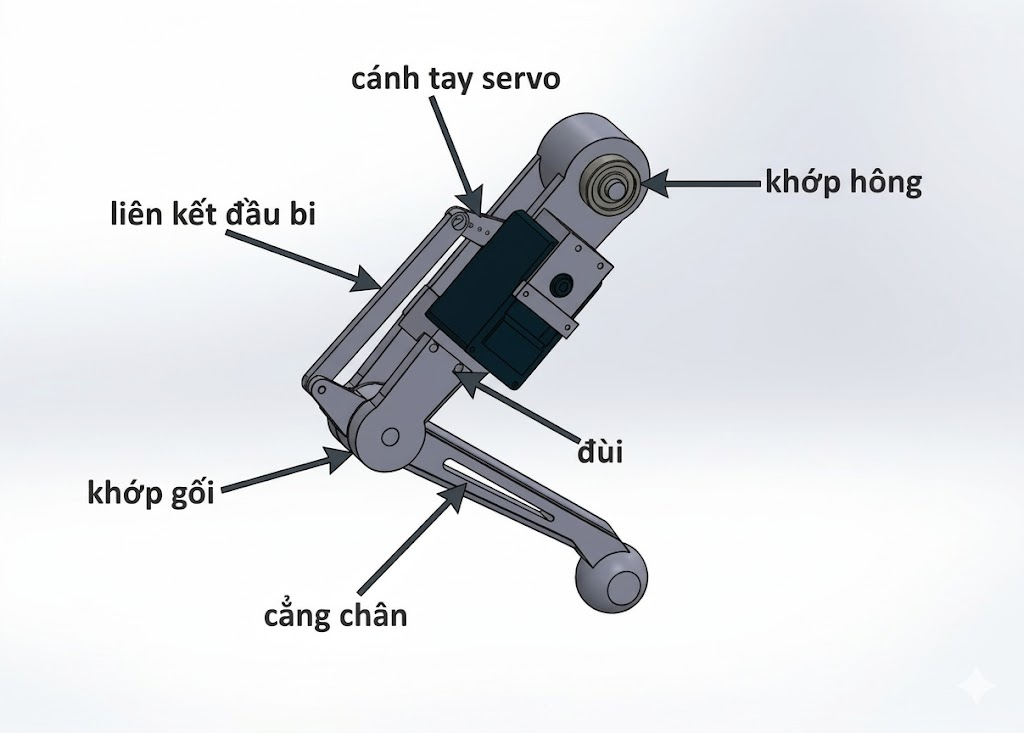
\includegraphics[width=0.6\textwidth]{hardware/single_leg_assembly.jpg}
    \caption{Cụm lắp ráp một chân đơn.}
    \label{fig14}
\end{figure}

Dựa trên cấu trúc chân của robot bốn chân, có thể thấy rằng cẳng chân là bộ phận dễ bị gãy và uốn cong nhất vì nó phải chịu trọng lượng của toàn bộ robot cũng như các lực nén khi tiếp xúc với mặt đất. 

Ở đây, lực tiếp xúc với mặt đất được đơn giản hóa chỉ gồm lực pháp tuyến $F_N$ và lực tiếp tuyến $F_\mu$ trong mặt phẳng thẳng đứng.

Khi cẳng chân quay quanh trục khớp gối, nếu bỏ qua ma sát tại khớp và ma sát tiếp xúc với mặt đất, mô-men tải ngoài lớn nhất có thể được xác định theo công thức:

\begin{equation}
    T_{\text{max}} = \eta F_N L_3 \sin(\alpha)
\end{equation}

trong đó $F_N$ là lực pháp tuyến, $L_3$ là khoảng cách từ trục khớp gối đến điểm tiếp xúc mặt đất, $\alpha$ là góc giữa cẳng chân và phương thẳng đứng và $\eta$ là hệ số tải động.

Tổng khối lượng robot được ước tính ở giai đoạn thiết kế xấp xỉ $M = 2.5\text{ kg}$.

Giả sử bốn chân chịu đều toàn bộ trọng lượng của robot trong trạng thái tĩnh, lực pháp tuyến được tính là:

\begin{equation}
    F_N = \frac{Mg}{4}
\end{equation}

Trong phân tích bền số học dưới đây, sử dụng các giá trị: chiều dài cẳng chân $L_3 = 0.125\text{ m}$, góc nghiêng $\alpha = 45^\circ$, và hệ số tải động $\eta = 1.6$.


\section{Lựa chọn cơ cấu chấp hành}
Việc lựa chọn cơ cấu chấp hành có ảnh hưởng lớn đến hiệu năng di chuyển của robot bốn chân. Do trọng lượng bản thân của robot, cơ cấu chấp hành cần tạo ra mô-men xoắn lớn, đáp ứng nhanh và có kích thước nhỏ gọn.

Động cơ không chổi than được sử dụng rộng rãi nhờ đặc tính động học vượt trội, tuy nhiên chúng thường có giá thành cao và kích thước lớn.

Vì trọng tâm chính của nghiên cứu này là triển khai và đánh giá sơ bộ thuật toán dáng đi trên mô hình robot kích thước để bàn, nên servo được lựa chọn làm nguồn truyền động.

Được trang bị khả năng phản hồi góc quay trực tiếp theo thời gian thực cùng tỷ số truyền bánh răng lớn, loại servo này cho phép vi điều khiển dễ dàng thực hiện điều khiển vòng kín. Điều này là nền tảng thiết yếu để chạy các node tính toán động học nghịch, giúp robot tự bù trừ sai số trong các thử nghiệm dáng đi phức tạp và tự cân bằng chính xác hơn.

Mẫu servo được sử dụng là ST3215 và ST3215-HS, như thể hiện ở Hình \ref{fig16}, và các thông số kỹ thuật cụ thể được trình bày trong Bảng \ref{tab:1}.

\begin{figure}[H]
    \centering
    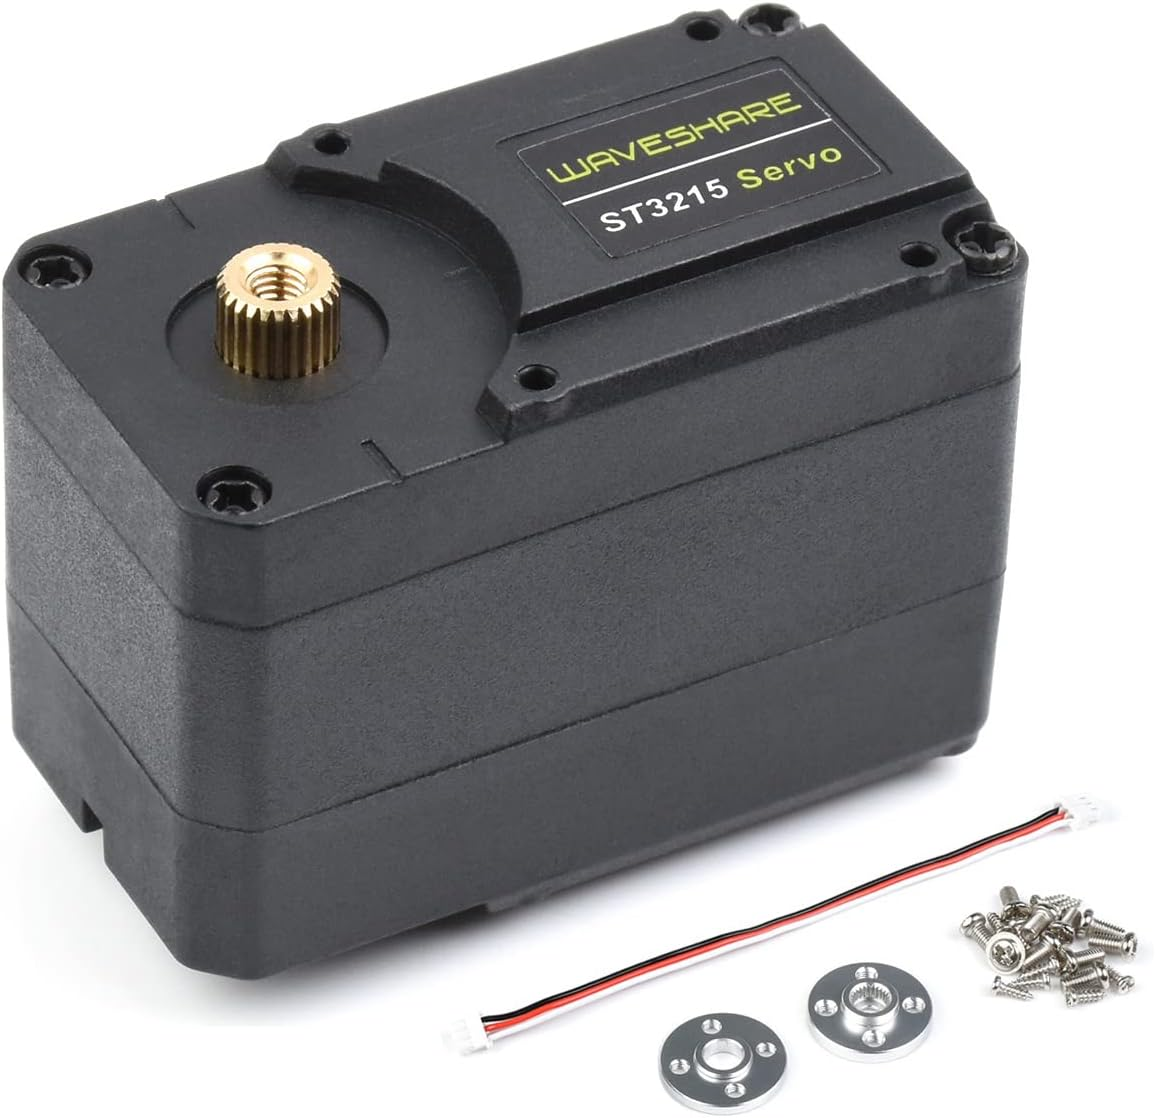
\includegraphics[width=0.6\textwidth]{hardware/servo_st3215.jpg}
    \caption{Cơ cấu chấp hành servo ST3215 dùng cho robot bốn chân.}
    \label{fig16}
\end{figure}

\begin{table}[htbp]
    \centering
    \caption{Thông số kỹ thuật của động cơ servo ST3215 và ST3215-HS.}
    \label{tab:1}
    \resizebox{\textwidth}{!}{% Thu nhỏ bảng vừa với chiều rộng trang giấy
        \begin{tabular}{l c c c c c c c}
            \toprule
            \textbf{Mẫu} & \textbf{Trọng lượng} & \textbf{\makecell{Kích thước \\ (L $\times$ W $\times$ H)}} & \textbf{\makecell{Điện áp \\ hoạt động}} & \textbf{\makecell{Tốc độ truyền \\ (Baudrate)}} & \textbf{\makecell{Phạm vi \\ góc quay}} & \textbf{Tốc độ tối đa} & \textbf{Lực xoắn tối đa} \\
            \midrule
            ST3215 & 69 g & \makecell{$45.2 \times 24.7 \times$ \\ $35.0$ mm} & 6.0 V -- 12.6 V & \textasciitilde 1 Mbps & \makecell{360$^\circ$ } & 0.222 s/60$^\circ$ (@12 V) & 30 kg$\cdot$cm (@12 V) \\
            \addlinespace % Thêm một khoảng trắng nhỏ giữa 2 hàng cho thoáng
            ST3215-HS & 68 g & \makecell{$45.2 \times 24.7 \times$ \\ $35.0$ mm} & 6.0 V -- 12.6 V & \textasciitilde 1 Mbps & \makecell{360$^\circ$ } & 0.094 s/60$^\circ$ (@12 V) & 20 kg$\cdot$cm (@12 V) \\
            \bottomrule
        \end{tabular}
    }
\end{table}

Để kiểm chứng mô-men xoắn định mức của servo đã chọn, tiến hành phân tích như sau. Dựa trên phân tích ở Mục 3.1.3, ảnh hưởng của mô-men xoắn lên cẳng chân là đáng kể nhất. Gọi góc giữa lực pháp tuyến tiếp xúc mặt đất $F_N$ và cẳng chân $L_3$ là $\alpha$. Như thể hiện trong Hình \ref{fig17}, mô-men do lực tiếp đất tác dụng lên khớp gối là:
\begin{equation}
    M_{\text{knee}} = \eta F_N L_3 \sin(\alpha)
\end{equation}
Mô-men này được cân bằng bởi lực truyền $F_t$ dọc theo thanh liên kết $CD$:
\begin{equation}
    M_{\text{knee}} = F_t L_{CB} \sin(\gamma)
\end{equation}
với $\gamma$ là góc giữa thanh liên kết $CD$ và cánh tay đòn $CB$. Mô-men tác dụng lên trục servo (qua cánh tay đòn $DE$) là:
\begin{equation}
    T_{\text{knee}} = F_t L_{DE} \sin(\beta)
\end{equation}
với $\beta$ là góc giữa thanh $CD$ và tay đòn $DE$. Trong thiết kế cơ cấu gần với hình bình hành, $\gamma \approx \beta$, do đó tỉ số $\sin(\beta)/\sin(\gamma) \approx 1$. Từ đó ta suy ra mô-men yêu cầu tại servo cẳng chân là:
\begin{equation}
    T_{\text{knee}} \approx \eta F_N L_3 \sin(\alpha) \frac{L_{DE}}{L_{CB}}
\end{equation}
Trong dáng đi trot, luôn có hai chân tiếp xúc mặt đất, do đó tải trọng lớn nhất tác dụng lên một chân là:
\begin{equation}
    F_N = \frac{Mg}{2}
\end{equation}
Thay các giá trị từ Bảng \ref{tab:2} với $M = 2.5\,\text{kg}$, $L_3 = 0.125\,\text{m}$, $L_{DE} = 0.024\,\text{m}$, $L_{CB} = 0.025\,\text{m}$, hệ số tải động $\eta = 1.6$, góc nghiêng $\alpha = 45^\circ$, và $g = 9.81\,\text{m/s}^2$ vào công thức, ta có $F_N = 12.26\,\text{N}$ và:
\begin{equation}
    T_{\text{knee}} \approx 1.6 \times 12.26 \times 0.125 \times \sin(45^\circ) \times \frac{0.024}{0.025} \approx 1.665\,\text{N}\cdot\text{m} \approx 17.0\,\text{kg}\cdot\text{cm}
\end{equation}

Giá trị này nhỏ hơn mô-men định mức $20\,\text{kg}\cdot\text{cm}$ của servo ST3215-HS, đảm bảo động cơ hoạt động an toàn theo thiết kế lý thuyết.

\begin{figure}[H]
    \centering
    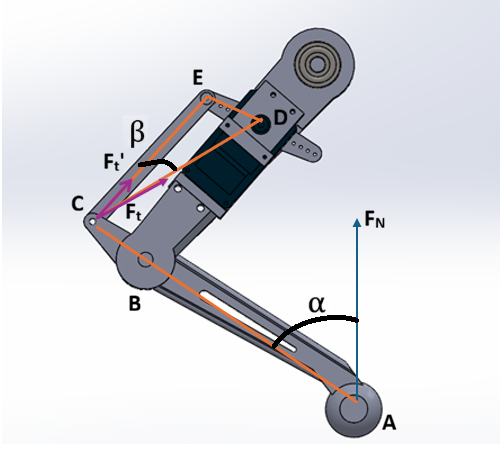
\includegraphics[width=0.6\textwidth]{hardware/servo_torque_analysis.png}
    \caption{Phân tích mô-men xoắn của cơ cấu chấp hành servo tại cẳng chân.}
    \label{fig17}
\end{figure}

\subsection{Phân tích mô-men khớp vai (Hip Roll)}

Trong thực tế vận hành, để duy trì khả năng thăng bằng và giảm chấn, chân robot không bao giờ duỗi thẳng hoàn toàn. Thay vào đó, phần đùi ($L_2$) và cẳng chân ($L_3$) luôn tạo với nhau một góc gập nhất định như thể hiện ở Hình \ref{fig18}. Việc tính toán mô-men xoắn cần sử dụng khoảng cách thực tế từ khớp hông đến bàn chân. 

Gọi $L_{hd}$ là khoảng cách hiệu dụng từ trục khớp hông đến điểm tiếp xúc mặt đất của bàn chân. Dựa trên định lý hàm số cosin cho tam giác tạo bởi đùi, cẳng chân và góc gập gối $\beta$, ta có:
\begin{equation}
    L_{hd} = \sqrt{L_2^2 + L_3^2 - 2L_2L_3\cos(\beta)}
\end{equation}

Dựa theo Bảng \ref{tab:2} với thiết kế $L_2 = 0.106\,\text{m}$ và $L_3 = 0.125\,\text{m}$, giả sử ở tư thế đi bộ trot tiêu chuẩn robot duy trì góc khuỵu gối $\beta = 90^\circ$ nhằm tối ưu lực bám. Chiều dài hiệu dụng lúc này là:
\begin{equation}
    L_{hd} = \sqrt{0.106^2 + 0.125^2 - 2(0.106)(0.125)\cos(90^\circ)} \approx 0.164\,\text{m}
\end{equation}

Tương tự phân tích trước, tải trọng lớn nhất tác dụng lên một chân là $F_N = 12.26\,\text{N}$, hệ số tải động $\eta = 1.6$, dẫn đến lực tác dụng tổng cộng là $\eta F_N = 19.62\,\text{N}$. 

Công thức tính mô-men xoắn cực đại cho khớp vai $T_{roll}$ theo góc dang chân $\theta_1$ được xác định dựa trên khoảng lệch ngàm $L_1$ và hình chiếu ngang của chiều dài chân hiệu dụng:
\begin{equation}
    T_{roll} = \eta F_N \big(L_1 \cos(\theta_1) + L_{hd} \sin(\theta_1)\big)
\end{equation}

Thay các thông số thiết kế ($L_1 = 0.026\,\text{m}$) vào phương trình, ta thu được:
\begin{equation}
    T_{roll} = 19.62 \times \big(0.026 \cos(\theta_1) + 0.164 \sin(\theta_1)\big) \quad \text{(N}\cdot\text{m)}
\end{equation}

Dựa vào phương trình trên, có thể đánh giá mô-men xoắn trong ba trường hợp tiêu biểu. Đầu tiên, khi $\theta_1 = 0^\circ$, mô-men tác dụng lên khớp vai chỉ xuất phát từ khoảng lệch ngàm cơ khí, đạt giá trị $T_{roll} = 19.62 \times 0.026 \approx 0.51\,\text{N}\cdot\text{m} \approx 5.2\,\text{kg}\cdot\text{cm}$. Tiếp theo, khi $\theta_1 = 15^\circ$, mô-men tăng lên mức $T_{roll} \approx 1.33\,\text{N}\cdot\text{m} \approx 13.5\,\text{kg}\cdot\text{cm}$, phản ánh trạng thái robot điều chỉnh tư thế rẽ với góc dang trung bình. Cuối cùng, khi $\theta_1 = 30^\circ$, mô-men đạt giá trị lớn nhất là $T_{roll} \approx 2.05\,\text{N}\cdot\text{m} \approx 20.9\,\text{kg}\cdot\text{cm}$, tương ứng với tình huống bất lợi khi chân dang rộng.

Giá trị mô-men cực đại $20.9\,\text{kg}\cdot\text{cm}$ vẫn nhỏ hơn định mức $30\,\text{kg}\cdot\text{cm}$ của servo ST3215, do đó khớp vai hoạt động trong vùng an toàn, đảm bảo hiệu năng và không gây quá tải nhiệt.

\begin{figure}[H]
    \centering
    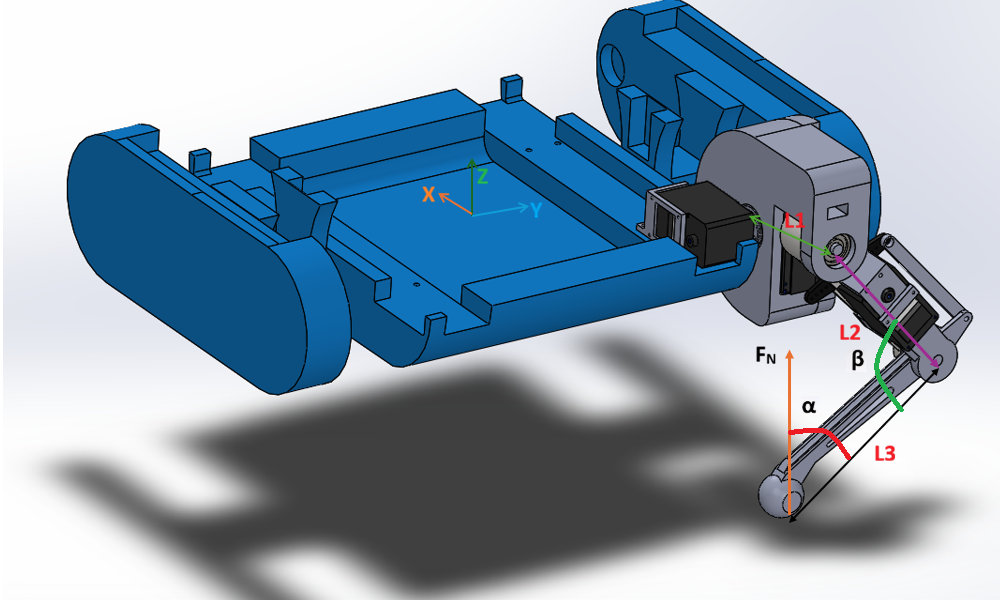
\includegraphics[width=0.6\textwidth]{hardware/free_body_diagram.png}
    \caption{Mô hình một chân của robot bốn chân.}
    \label{fig18}
\end{figure}

\subsection{Phân tích mô-men khớp hông (Hip Pitch)}

Tương tự quy trình đánh giá ở khớp vai, mô-men xoắn yêu cầu cực đại đối với khớp hông (Pitch) được xác định thông qua chiều dài sải bước hiệu dụng của robot. Trong mặt phẳng dọc, cánh tay đòn tạo ra mô-men phụ thuộc vào độ vươn xa của bàn chân theo phương ngang. Gọi $\alpha$ là góc nghiêng của chân (đường nối từ trục khớp hông đến bàn chân) so với phương thẳng đứng. Phương trình tổng quát tính mô-men xoắn cho khớp hông là:
\begin{equation}
    T_{pitch} = \eta F_N L_{hd} \sin(\alpha)
\end{equation}

Sử dụng khoảng cách hiệu dụng $L_{hd} = 0.164\,\text{m}$ và lực tải $\eta F_N = 19.62\,\text{N}$ đã xác định:
\begin{equation}
    T_{pitch} = 19.62 \times 0.164 \sin(\alpha) = 3.218 \sin(\alpha) \quad \text{(N}\cdot\text{m)}
\end{equation}

Phân tích quỹ đạo chuyển động cho thấy:
Phân tích quỹ đạo chuyển động cho thấy ba trạng thái chịu tải đặc trưng. Tại tư thế đứng thẳng chân ($\alpha = 0^\circ$), trọng lượng truyền dọc theo chân nên khớp hông hoàn toàn không chịu tải uốn ($T_{pitch} = 0$). Trong trường hợp khi chân bước với góc $\alpha = 15^\circ$, mô-men tại khớp hông đạt $T_{pitch} = 3.218 \sin(15^\circ) \approx 0.83\,\text{N}\cdot\text{m} \approx 8.5\,\text{kg}\cdot\text{cm}$; đây được xem là vùng tải nhẹ và rất thuận lợi cho động cơ hoạt động. Tuy nhiên, khi góc bước mở rộng lên $\alpha = 45^\circ$, mô-men tăng lên mức $T_{pitch} = 3.218 \sin(45^\circ) \approx 2.27\,\text{N}\cdot\text{m} \approx 23.2\,\text{kg}\cdot\text{cm}$, tương ứng với trạng thái vươn dài chân để leo dốc hoặc vượt chướng ngại vật.

Giá trị cực đại này vẫn nhỏ hơn giới hạn mô-men $30\,\text{kg}\cdot\text{cm}$ của servo ST3215, xác nhận rằng việc lựa chọn động cơ ST3215 cho khớp hông là hoàn toàn phù hợp và đảm bảo độ an toàn cao.

\subsection{Thiết kế tổng thể}

Thiết kế tổng thể của robot bốn chân được thể hiện trong Hình \ref{fig19}, với tổng cộng 12 bậc tự do và cấu hình chân full-elbow. Ở đây, cả bốn chân đều giống hệt nhau về cấu trúc và kích thước nhằm tạo thuận lợi cho việc điều khiển.

Khớp hông được kết nối trực tiếp với servo ở cả hai bậc tự do để đơn giản hóa cấu trúc bên trong, trong khi khớp gối được thiết kế sử dụng cơ cấu tay đòn servo kết hợp với thanh liên kết nhằm giảm quán tính của chân.

Các tham số chính của hệ thống được trình bày trong Bảng \ref{tab:2}.

\begin{figure}[H]
    \centering
    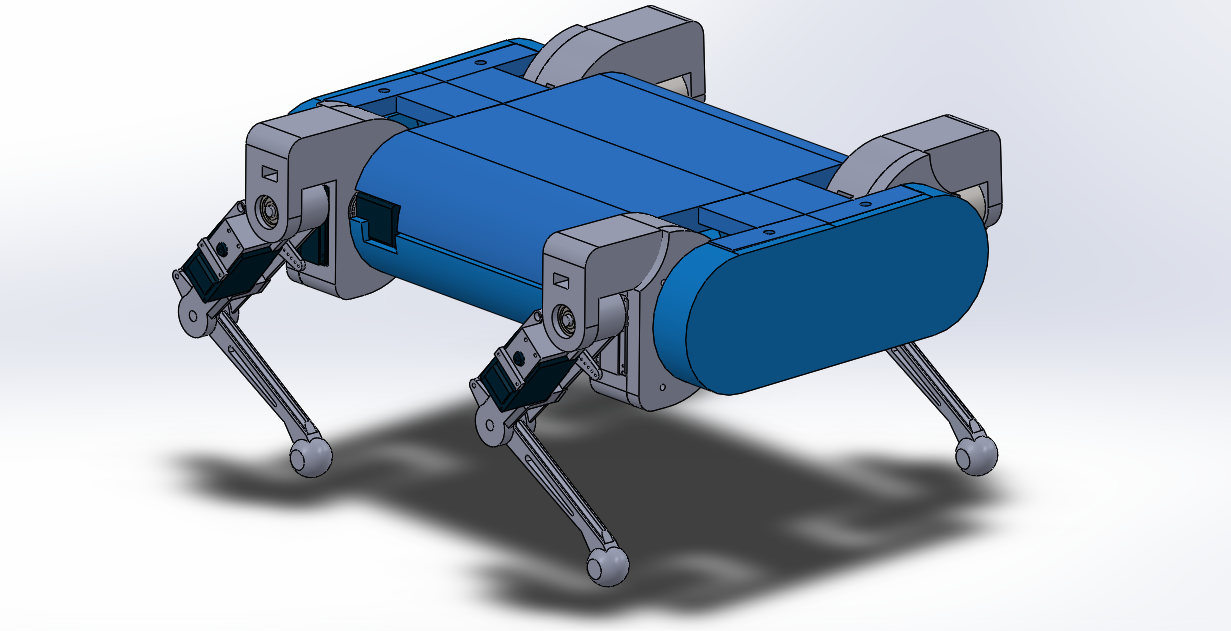
\includegraphics[width=0.6\textwidth]{hardware/preview_design.png }
    \caption{3D thiết kế robot Dog}
    \label{fig19}
\end{figure}

\begin{table}[h]
\centering
\caption{Các thông số chính của robot bốn chân}
 \label{tab:2}
\begin{tabular}{ccccccc}
\toprule
Chiều dài & Chiều rộng & Chiều cao & \makecell{Chiều dài\\hông\\$L_1$} & \makecell{Chiều dài\\đùi\\$L_2$} & \makecell{Chiều dài\\cẳng chân\\$L_3$} & \makecell{Bậc\\tự do} \\
\midrule
209 mm & 191 mm & 185 mm & 26 mm & 106 mm & 125 mm & 12 \\
\bottomrule
\end{tabular}
\end{table}

\section{Tổng quan về kiến trúc hệ thống }

Kiến trúc phần cứng của hệ thống robot bốn chân được xây dựng nhằm mục tiêu cung cấp nguồn năng lượng ổn định, đảm bảo khả năng xử lý thuật toán phức tạp theo thời gian thực và điều khiển đồng bộ nhiều cơ cấu chấp hành. Sơ đồ kết nối phần cứng tổng thể của mô hình thực nghiệm được thể hiện chi tiết trong Hình~\ref{fig30}.

\begin{figure}[H]
    \centering
    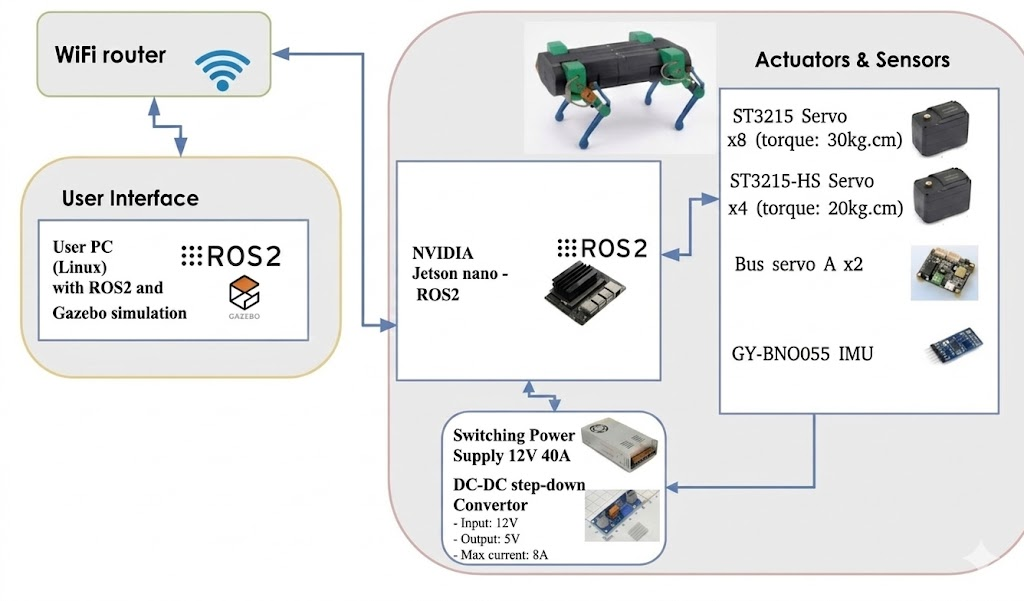
\includegraphics[width=\textwidth]{architecture/system_overview.jpeg}
    \caption{Sơ đồ kiến trúc tổng thể của hệ thống robot bốn chân.}
    \label{fig30}
\end{figure}

Hình~\ref{fig:real_robot} trình bày mô hình robot bốn chân thực tế đã được chế tạo và lắp ráp hoàn chỉnh. Robot sử dụng khung thân và các chi tiết chân được gia công bằng công nghệ in 3D FDM với vật liệu PLA, tích hợp 12 động cơ bus servo ST3215 tại các khớp, cảm biến IMU BNO055 gắn trên thân và máy tính nhúng Jetson Nano làm bộ xử lý trung tâm.

\begin{figure}[H]
    \centering
    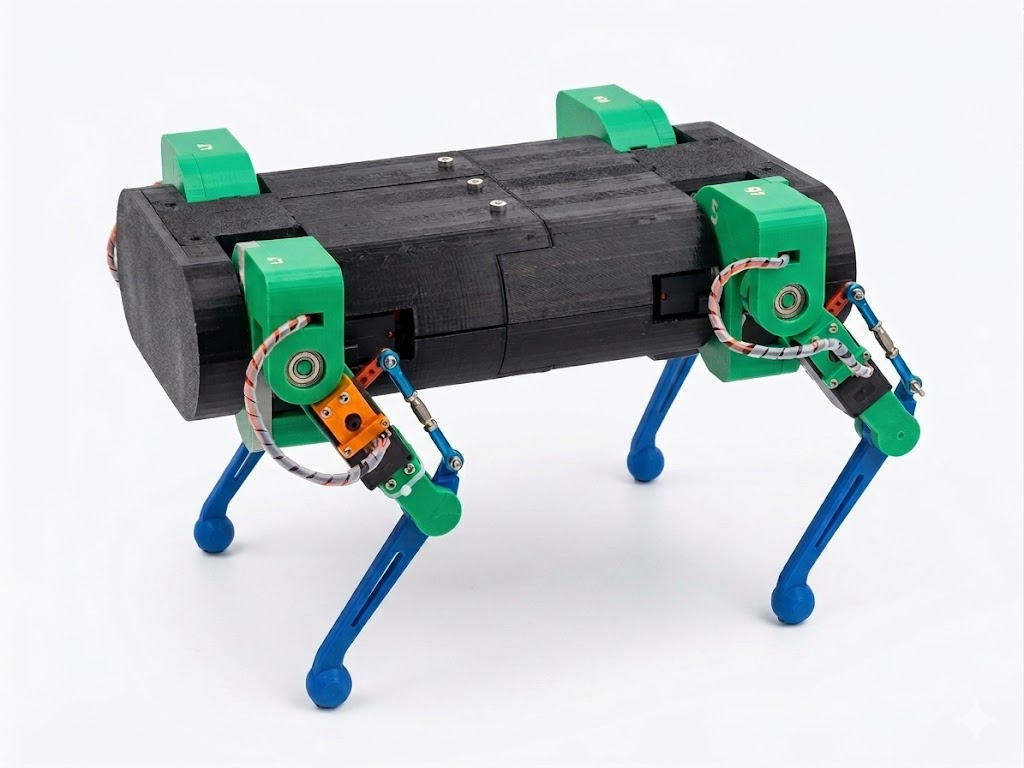
\includegraphics[width=0.85\textwidth]{real_robot/quadrupedrobot.jpeg}
    \caption{Mô hình robot bốn chân thực tế đã được chế tạo và lắp ráp hoàn chỉnh.}
    \label{fig:real_robot}
\end{figure}

\subsection{Khối xử lý trung tâm }

Bộ xử lý trung tâm phải đáp ứng khả năng tính toán các bài toán phức tạp như động học nghịch, quy hoạch quỹ đạo và xử lý dữ liệu cân bằng theo thời gian thực. Do đó, máy tính nhúng Jetson Nano Developer Kit B01 \cite{jetson_nano} đã được lựa chọn. Vi xử lý Quad-core ARM Cortex-A57 cùng hệ điều hành Ubuntu mang lại sức mạnh vượt trội, cho phép triển khai hệ sinh thái ROS~2 và các thư viện toán học phức tạp một cách dễ dàng.

\begin{figure}[H]
    \centering
    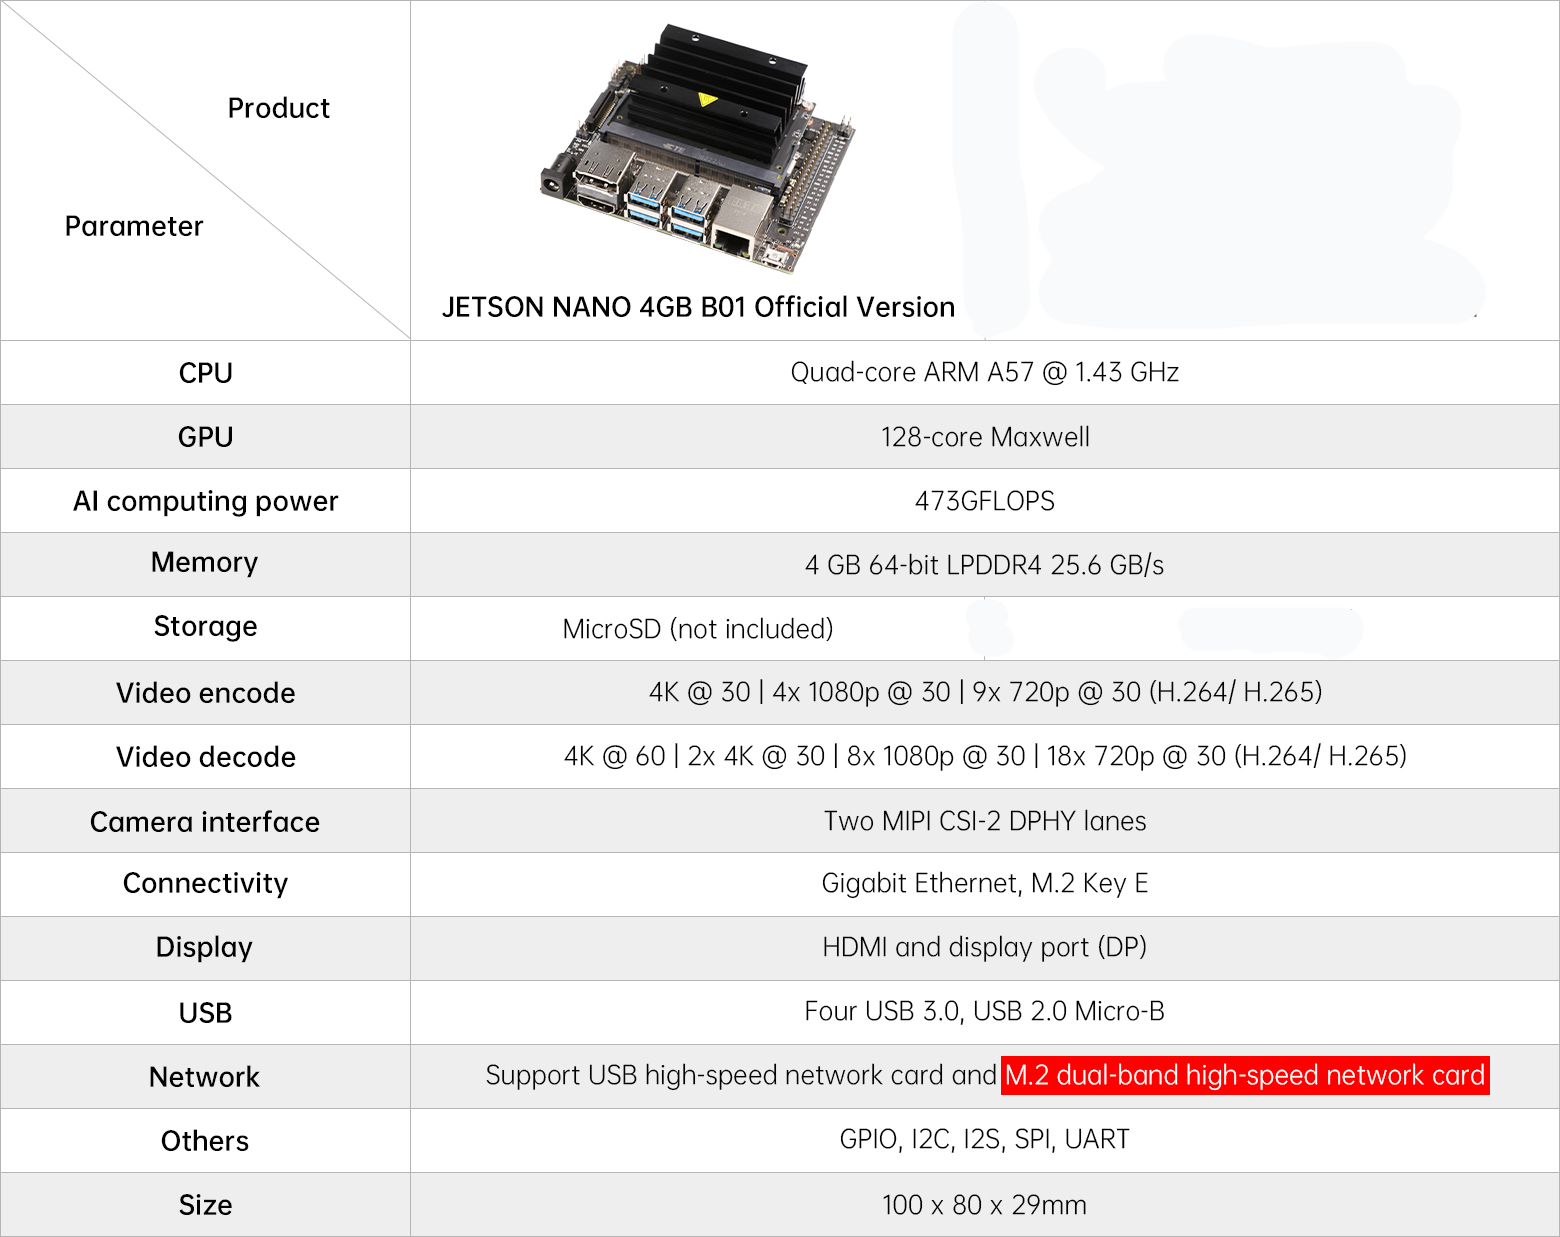
\includegraphics[width=0.8\textwidth]{hardware/jetson_b01_specs.png} 
    \caption{Thông số kỹ thuật Jetson Nano B01}
    \label{fig34}
\end{figure}

Jetson Nano thực thi vòng lặp điều khiển chính, quản lý 12 động cơ servo và đọc dữ liệu từ module cảm biến IMU. Thiết bị thiết lập giao tiếp UART tốc độ cao với hai mạch Bus Servo Adapter (A) nhằm phân phối tín hiệu điều khiển nối tiếp đến các cơ cấu chấp hành, giúp giảm tải dòng điện và tối giản hóa sơ đồ đi dây vật lý. 

\subsection{Hệ thống Cung cấp Nguồn điện}

Trong giai đoạn phát triển và tinh chỉnh động học, hệ thống yêu cầu một nguồn điện có khả năng cung cấp dòng xả lớn và liên tục để tránh hiện tượng sụt áp khi 12 động cơ servo cùng khởi chạy. Do đó, nguồn xung tổ ong 12~V - 40~A (480~W) đã được lựa chọn. Thiết bị này đảm bảo cung cấp điện áp 12~V ổn định, tối ưu hóa hiệu suất của các servo ST3215 và hỗ trợ tốt cho quá trình thử nghiệm dài hạn trong phòng thí nghiệm.

Việc lựa chọn nguồn xung tổ ong 12~V - 40~A (480~W) được dựa trên tính toán dòng điện tiêu thụ của 12 động cơ servo ST3215:

Dòng điện không tải/hoạt động bình thường : Khoảng 300~mA - 600~mA / servo (tại 12~V).
    
Dòng điện khởi động/giữ tải lớn nhất ($I_{stall}$): Khoảng 2.7~A / servo (tại 12~V).

Trong trường hợp xấu nhất khi robot khởi động hoặc thực hiện động tác nâng toàn thân, giả sử cả 12 servo đều chịu tải lớn, tổng dòng điện tức thời ($I_{total}$) là:

$$I_{total} = N_{servo} \times I_{stall} = 12 \times 2.7 = 32.4A$$

Theo đó, tổng công suất tiêu thụ điện tối đa ($P_{total}$) của riêng hệ thống cơ cấu chấp hành là:

$$P_{total} = I_{total} \times U = 32.4 \times 12 = 388.8W$$

Để đảm bảo an toàn và tuổi thọ cho linh kiện, tránh sụt áp nguồn khi ép tải, hệ số an toàn ($k$) thường được chọn từ 1.2 đến 1.5. Ở đây nhóm chọn hệ số $k = 1.2$, ta có yêu cầu công suất nguồn cấp tối thiểu phải đạt:

$$P_{source} \ge P_{total} \times k = 388.8 \times 1.2 = 466.56W$$

Việc lựa chọn nguồn xung tổ ong 12~V - 40~A (công suất cực đại 480~W) là hoàn toàn chính xác và bám sát với tính toán lý thuyết ($466.56~W \le 480~W$). Mức công suất và dòng điện này đảm bảo khả năng đáp ứng dòng xả cao ngay cả khi robot hoạt động ở trạng thái tải nặng nhất mà không gây sụt áp hệ thống, giúp vi xử lý trung tâm Jetson Nano và các module không bị reset đột ngột.

\begin{table}[H] % <--- Chỗ này bắt buộc phải là [H]
\centering
\caption{Thông số kỹ thuật}
\renewcommand{\arraystretch}{1.3}
\begin{tabular}{p{0.3\textwidth} p{0.6\textwidth}}
\toprule
\textbf{Thuộc tính} & \textbf{Giá trị} \\
\midrule
Điện áp ngõ ra & 12~V \\
Dòng điện ngõ ra & 40-49A \\
Số điện áp ra & 1 \\
Điện áp ngõ vào & 220VAC \\
Series & Khác \\
Công suất & 400-499W \\
Cách gắn & Gắn sàn \\
Vỏ bọc & Vỏ kim loại \\
\bottomrule
\end{tabular}
\end{table}

Mức công suất 480W cung cấp một biên độ an toàn dư dả để cấp nguồn song song cho cả cụm 12 servo và máy tính nhúng Jetson Nano. Mặc dù giới hạn phạm vi di chuyển bởi dây cáp nguồn, đây là giải pháp kinh tế và đáng tin cậy nhất cho nguyên mẫu thử nghiệm tại chỗ.

\subsection{Bus Servo Adapter (A)}

Các động cơ servo ST3215 được sử dụng trong thiết kế hoạt động dựa trên chuẩn giao tiếp nối tiếp bán song công (half-duplex UART). Để máy tính nhúng Jetson Nano có thể điều khiển đồng thời cả 12 động cơ này một cách an toàn và tối ưu, hệ thống sử dụng hai mạch chuyển đổi tín hiệu Bus Servo Adapter (A). Mạch Adapter đóng vai trò trung gian, chuyển đổi tín hiệu UART tiêu chuẩn từ Jetson Nano (thông qua cổng USB) thành tín hiệu bus nối tiếp cấp cho các động cơ. 

Mặc dù về mặt lý thuyết, một mạch Bus Servo Adapter (A) có thể điều khiển tối đa 253 động cơ nối tiếp, nhưng trong thực tế, dòng điện khởi động của 12 động cơ ST3215 có thể lên đến 32.4A. Việc sử dụng song song hai mạch Adapter mang lại những lợi ích thiết thực:
Việc sử dụng song song hai mạch Adapter mang lại hai lợi ích thiết thực chính. Lợi ích thứ nhất là khả năng phân tán dòng điện hiệu quả; nhờ đó, mỗi mạch Adapter chỉ cần chịu tải dòng điện cho 6 động cơ (khoảng 16.2A tối đa), giúp giảm thiểu đáng kể rủi ro quá tải nhiệt và cháy nổ cho bản mạch in (PCB) của Adapter so với việc phải gánh toàn bộ tải. Lợi ích thứ hai là khả năng tối ưu hóa sơ đồ đi dây; thông qua việc phân chia hệ thống thành hai cụm độc lập (như nửa trái và nửa phải của robot), kết nối vật lý trở nên gọn gàng, logic và thuận tiện hơn rất nhiều cho quá trình kiểm tra cũng như bảo trì.

Thông qua các giao thức truyền thông và tập lệnh được định nghĩa sẵn, hệ thống có thể điều khiển hiệu quả các biến số như: góc quay, tốc độ di chuyển, giới hạn tải, cũng như đọc các tín hiệu phản hồi về nhiệt độ, điện áp và vị trí thực tế của từng động cơ.

\begin{figure}[H]
    \centering
    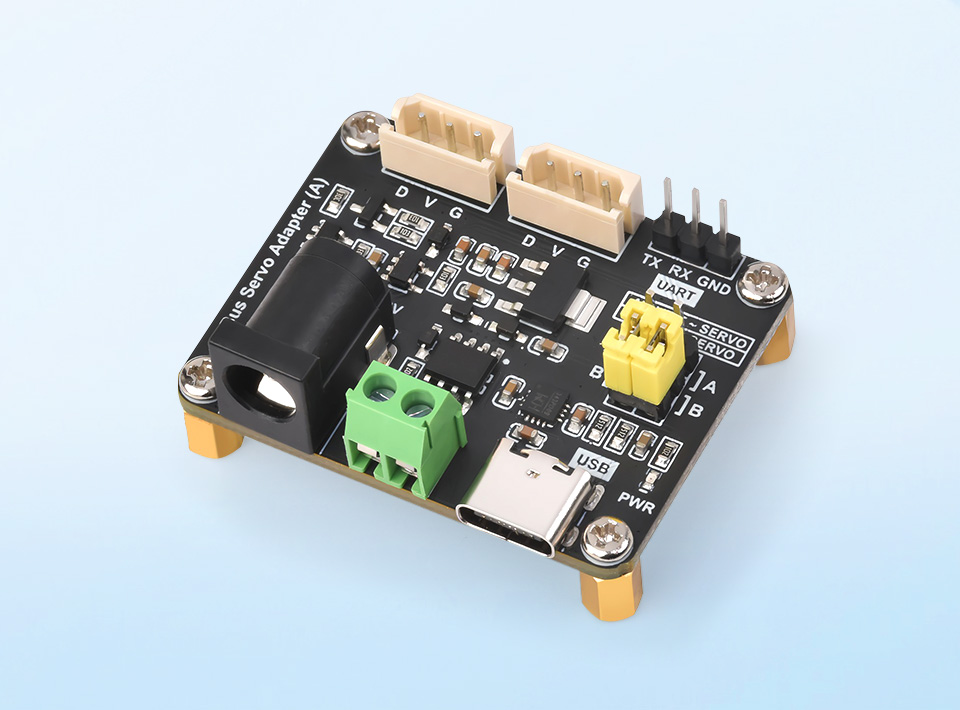
\includegraphics[width=0.6\textwidth]{hardware/bus_servo_adapter.jpg} 
    \caption{Bus Servo Adapter (A)}
    \label{fig36}
\end{figure}

\begin{table}[H]
    \centering
    \caption{Thông số kỹ thuật mạch Bus Servo Adapter (A)}
    \label{tab:adapter_specs}
    \renewcommand{\arraystretch}{1.5} % Tăng độ rộng giữa các hàng cho thoáng và đẹp giống ảnh
    \begin{tabular}{p{0.35\textwidth} p{0.5\textwidth}}
        \hline
        \textbf{Power Supply} & DC 9 $\sim$ 12.6V (ST series servo) \\ \hline
        \textbf{Power supply connector} & 5.5 $\times$ 2.1mm DC \\ \hline
        \textbf{communication interface} & UART \\ \hline
        \textbf{Dimensions} & 42.00 $\times$ 33.00mm \\ \hline
        \textbf{Mounting hole size} & 2.50mm \\ \hline
        \textbf{Mounting hole spacing} & 37.00 $\times$ 28.00mm \\ \hline
    \end{tabular}
\end{table}

\subsection{Bộ đo lường quán tính }

Module IMU (Inertial Measurement Unit) đóng vai trò cốt lõi trong hệ thống phản hồi thăng bằng của robot. Thay vì sử dụng các cảm biến quán tính thô, nghiên cứu này ứng dụng module GY-BNO055 \cite{bno055} --- một board mạch breakout nhỏ gọn được thiết kế trên nền tảng chip cảm biến BNO055 của Bosch Sensortec. Module tích hợp sẵn gia tốc kế 3 trục, con quay hồi chuyển 3 trục, từ kế 3 trục và đặc biệt là một vi xử lý ARM Cortex-M0+ 32-bit chạy thuật toán kết hợp cảm biến (Sensor Fusion) độc quyền của Bosch, cho phép xuất trực tiếp dữ liệu định hướng tuyệt đối mà không cần bộ lọc ngoại vi.

\begin{figure}[H]
\centering
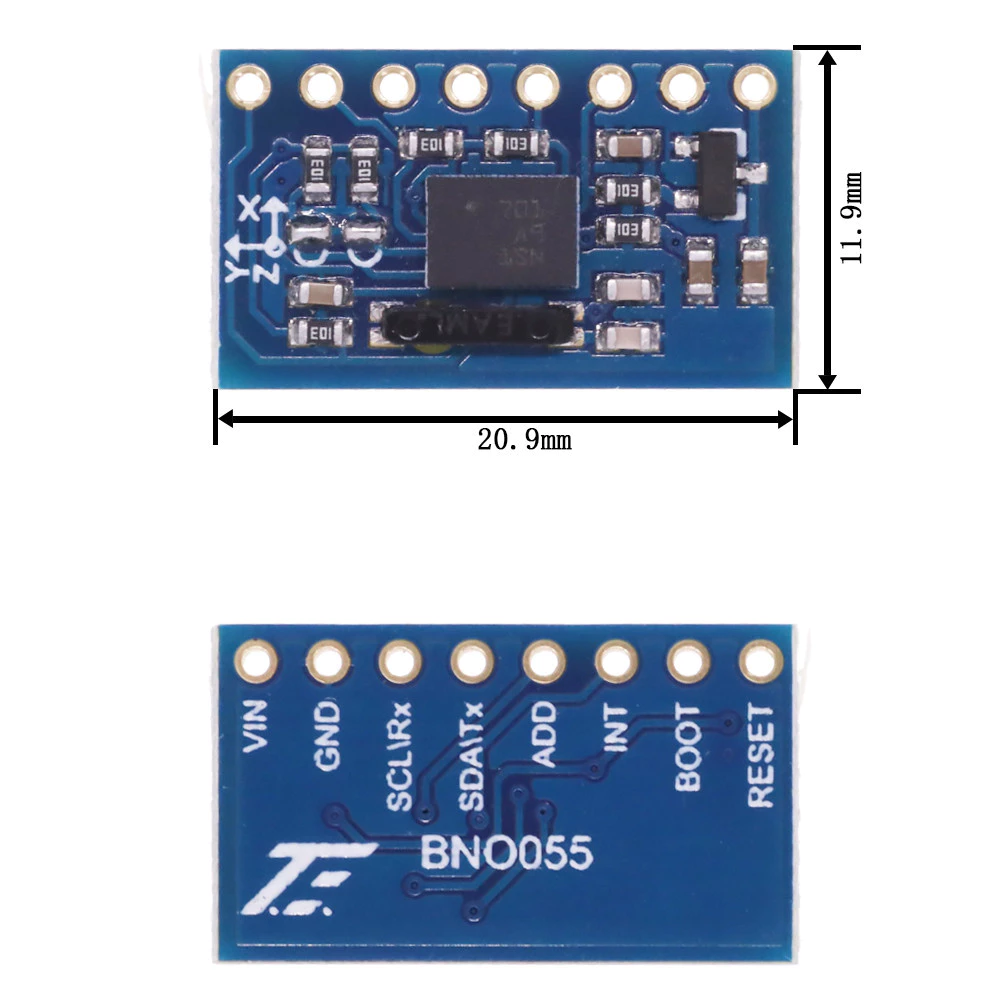
\includegraphics[width=0.55\textwidth]{hardware/imu_bno055.png}
\caption{Module cảm biến 9 trục thông minh GY-BNO055 (mặt trước và mặt sau)}
\label{fig37}
\end{figure}

Module GY-BNO055 sở hữu kích thước cực kỳ nhỏ gọn (20,9~mm $\times$ 11,9~mm), rất phù hợp để gắn trực tiếp lên khung thân robot mà không chiếm nhiều không gian. Board mạch được bố trí 8 chân tín hiệu gồm: VIN (nguồn cấp), GND (mass), SCL/Rx (xung nhịp I2C hoặc nhận UART), SDA/Tx (dữ liệu I2C hoặc phát UART), ADD (chọn địa chỉ I2C), INT (ngắt ngoài), BOOT (chế độ nạp firmware) và RESET (khởi động lại phần cứng). Mạch tích hợp sẵn bộ ổn áp nội cho phép cấp nguồn linh hoạt từ 3,3V đến 5V qua chân VIN.

Về mặt kiến trúc phần cứng, nhóm đã tối ưu hóa hệ thống bằng cách loại bỏ hoàn toàn vi điều khiển trung gian như cấu trúc dùng STM32. Nền tảng phát triển giờ đây được triển khai trực tiếp trên môi trường hệ điều hành Linux của Jetson Nano. Cảm biến BNO055 được kết nối và giao tiếp thẳng với Jetson Nano thông qua bus I2C (sử dụng hai chân SCL và SDA). Việc lập trình thu thập dữ liệu được thực hiện bằng ngôn ngữ Python. Sự thay đổi này không chỉ giúp giảm thiểu đáng kể độ trễ truyền dữ liệu mà còn tối giản hóa độ phức tạp của việc đi dây phần cứng.

Khác với các cảm biến truyền thống (như MPU6050) dễ bị nhiễu từ môi trường và đòi hỏi người lập trình phải tự xây dựng các bộ lọc toán học phức tạp (như Complementary Filter hay Kalman Filter) trên máy tính chủ, BNO055 xử lý toàn bộ khối lượng công việc này ở cấp độ phần cứng nội bộ. Tính năng Sensor Fusion của BNO055 tự động tính toán và xuất trực tiếp dữ liệu định hướng dưới dạng các góc Euler (Roll, Pitch, Yaw) hoặc Quaternion với độ chính xác cao và tần số cập nhật nhanh. Do đó, bài toán của nhóm được chuyển từ việc ``viết bộ lọc nhiễu'' sang việc quản lý quy trình tự hiệu chuẩn của cảm biến.
\begin{table}[H]
\centering
\caption{Thông số kỹ thuật module cảm biến GY-BNO055}
\label{tab:bno055_specs}
\renewcommand{\arraystretch}{1.3}
\begin{tabular}{p{0.3\textwidth} p{0.55\textwidth}}
\toprule
\textbf{Thông số} & \textbf{Giá trị} \\
\midrule
Chip cảm biến & Bosch BNO055 (SiP -- System in Package) \\
Số trục đo & 9 trục (Accelerometer + Gyroscope + Magnetometer) \\
Điện áp hoạt động & 3.3V -- 5V (qua chân VIN, tích hợp bộ ổn áp nội) \\
Chuẩn giao tiếp & I2C / UART (chọn qua chân BOOT) \\
Địa chỉ I2C mặc định & 0x28 (chân ADD = LOW); 0x29 (chân ADD = HIGH) \\
Gia tốc kế (Accelerometer) & $\pm$2g / $\pm$4g / $\pm$8g / $\pm$16g \\
Con quay hồi chuyển (Gyroscope) & $\pm$125$^\circ$/s đến $\pm$2000$^\circ$/s \\
Từ kế (Magnetometer) & $\pm$1300$\mu$T (trục x,y); $\pm$2500$\mu$T (trục z) \\
Bộ xử lý tích hợp & ARM Cortex-M0+ (chạy thuật toán Sensor Fusion) \\
Dữ liệu đầu ra & Quaternion, góc Euler, vector trọng lực, gia tốc tuyến tính \\
Tần số cập nhật Fusion & Lên đến 100 Hz \\
Kích thước mạch & 20,9 $\times$ 11,9 mm \\
Số chân tín hiệu & 8 (VIN, GND, SCL/Rx, SDA/Tx, ADD, INT, BOOT, RESET) \\
Nhiệt độ hoạt động & $-40^\circ$C đến $+85^\circ$C \\
\bottomrule
\end{tabular}
\end{table}
\subsection{Mạch Giảm Áp}

Máy tính nhúng Jetson Nano yêu cầu một nguồn DC 5~V ổn định và có khả năng tiêu thụ dòng điện lên đến 4~A khi xử lý các tác vụ nặng. Để đáp ứng yêu cầu này, mạch giảm áp xung XL4015 5~A 75~W được sử dụng để chuyển đổi điện áp 12~V từ nguồn tổ ong xuống 5~V. XL4015 mang lại hiệu suất chuyển đổi cao (lên đến 96\%), dòng đầu ra tối đa 5~A, cùng các tính năng bảo vệ ngắn mạch và quá nhiệt, đảm bảo an toàn tuyệt đối cho Jetson Nano.

\begin{figure}[H]
    \centering
    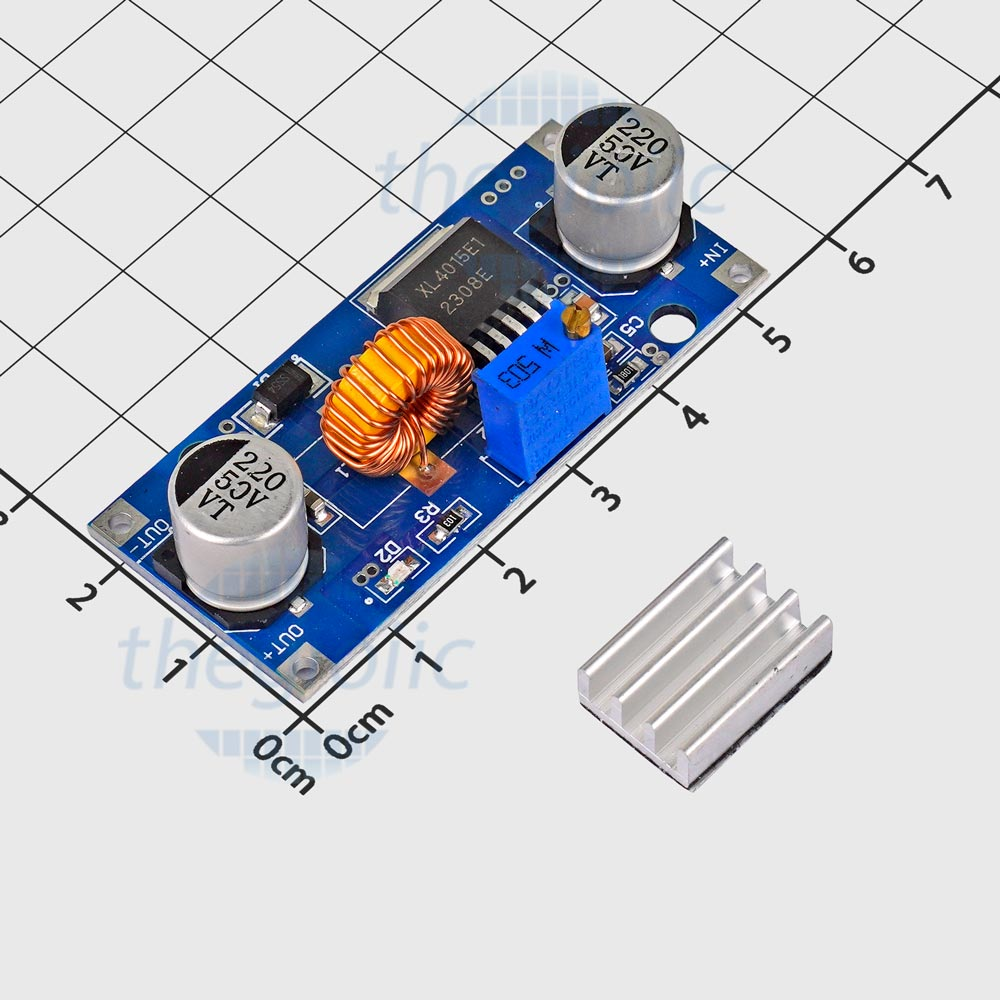
\includegraphics[width=0.6\textwidth]{hardware/buck_converter.jpg} 
    \caption{Mạch giảm áp XL4015 5A 75W}
    \label{fig38}
\end{figure}

Các thông số kỹ thuật chi tiết của mạch giảm áp XL4015 được trình bày cụ thể trong Bảng \ref{tab:xl4015_specs}. Mức điện áp ngõ ra đã được chúng em tinh chỉnh qua biến trở tích hợp trên mạch để đạt chính xác mức 5.0V - 5.1V nhằm bù trừ sụt áp trên dây dẫn trước khi cấp vào Jetson Nano.

\begin{table}[H]
    \centering
    \caption{Thông số kỹ thuật mạch giảm áp XL4015 5A 75W}
    \label{tab:xl4015_specs}
    \renewcommand{\arraystretch}{1.5} 
    \begin{tabular}{p{0.3\textwidth} p{0.55\textwidth}}
        \hline
        \textbf{Điện áp ngõ vào} & 5 $\sim$ 32 VDC \\ \hline
        \textbf{Điện áp ngõ ra} & 1.25 $\sim$ 30 VDC (Tinh chỉnh về 5V cấp cho vi xử lý) \\ \hline
        \textbf{Dòng ngõ ra} & 0 $\sim$ 5A \\ \hline
        \textbf{Công suất ngõ ra} & 75W \\ \hline
        \textbf{Nhiệt độ làm việc} & -40 $\sim$ +85$^\circ$C \\ \hline
        \textbf{Tần số hoạt động} & 180KHz \\ \hline
        \textbf{Hiệu suất tối đa} & 96\% \\ \hline
        \textbf{Bảo vệ ngắn mạch} & Có (giới hạn 8A) \\ \hline
        \textbf{Bảo vệ quá nhiệt} & Có \\ \hline
    \end{tabular}
\end{table}


\subsection{Cơ cấu chấp hành: Động cơ Bus Servo ST3215}

Việc lựa chọn cơ cấu chấp hành có ảnh hưởng trực tiếp đến hiệu năng di chuyển, khả năng giữ thăng bằng và độ phức tạp của hệ thống phần cứng robot bốn chân. Trong nghiên cứu này, động cơ Bus Servo ST3215 và phiên bản tốc độ cao ST3215-HS \cite{waveshare_st3215} đã được lựa chọn làm thiết bị truyền động cho toàn bộ 12 bậc tự do của robot. 

Để làm rõ tính ưu việt và lý do lựa chọn công nghệ truyền động này cho mô hình nguyên mẫu, nhóm đã tiến hành đánh giá và so sánh dòng động cơ Bus Servo nối tiếp với hai loại cơ cấu chấp hành phổ biến khác: Động cơ Servo điều khiển bằng xung PWM truyền thống và Động cơ không chổi than (BLDC).

\begin{table}[H]
\centering
\caption{Bảng so sánh các loại cơ cấu chấp hành áp dụng cho Robot bốn chân}
\label{tab:motor_comparison}
\renewcommand{\arraystretch}{1.3}
\resizebox{\textwidth}{!}{
\begin{tabular}{|p{0.2\linewidth}|p{0.2\linewidth}|p{0.2\linewidth}|p{0.25\linewidth}|}
\hline
\textbf{Tiêu chí} & \textbf{Động cơ Servo PWM truyền thống} & \textbf{Động cơ BLDC (Tích hợp Driver)} & \textbf{Động cơ Bus Servo nối tiếp} \\ \hline
\textbf{Giao thức điều khiển} & Xung PWM (Đơn hướng) & CAN / RS485 (Song công) & UART bán song công (Half-duplex) \\ \hline
\textbf{Hệ thống dây dẫn} & Rất phức tạp (Mỗi motor 1 dây tín hiệu riêng) & Tối giản (Nối tiếp chuỗi - Daisy chain) & Tối giản (Nối tiếp chuỗi - Daisy chain) \\ \hline
\textbf{Khả năng phản hồi (Feedback)} & Không có & Vị trí, tốc độ, dòng điện, nhiệt độ (FOC) & Vị trí thực tế, tốc độ, tải, nhiệt độ, điện áp \\ \hline
\textbf{Mô-men xoắn} & Thường ở mức thấp đến trung bình & Rất cao & Cao (Tối ưu trong tầm giá) \\ \hline
\textbf{Khối lượng \& Kích thước} & Nhẹ & Nặng, cồng kềnh & Gọn nhẹ \\ \hline
\textbf{Giá thành} & Rất thấp & Rất cao & Trung bình - Hợp lý \\ \hline
\textbf{Độ phù hợp} & Thấp (Do không có phản hồi và thiếu lực) & Thấp (Dư thừa công suất, chi phí quá cao) & \textbf{Rất cao (Đạt điểm cân bằng tối ưu)} \\ \hline
\end{tabular}
}
\end{table}

Sau khi xác định kiến trúc truyền động tối ưu là sử dụng Bus Servo nối tiếp thay vì Servo PWM hay động cơ BLDC, nhóm đã tiến hành khảo sát và đánh giá các dòng Bus Servo phổ biến trên thị trường để tìm ra phương án phù hợp nhất cho hệ thống 12 bậc tự do của robot. Tuy nhiên, để có cái nhìn trực quan và toàn diện nhất, nhóm cũng đưa vào bảng so sánh một đại diện tiêu biểu của dòng Servo PWM là JX Servo PDI-HV5932MG 30KG -- loại động cơ có lực xoắn lớn, góc quay $180^{\circ}$, vốn rất phổ biến trong các dự án sinh viên để thấy rõ sự khác biệt giữa hai công nghệ.

Bốn đại diện tiêu biểu được đưa ra so sánh bao gồm: JX PDI-HV5932MG (Servo PWM), Hiwonder LX-16A, Waveshare ST3215 và Dynamixel XL430-W250-T.

\begin{table}[H]
\centering
\caption{So sánh các dòng Servo phổ biến trên thị trường}
\label{tab:bus_servo_comparison}
\renewcommand{\arraystretch}{1.3}
\resizebox{\textwidth}{!}{
\begin{tabular}{|p{0.14\linewidth}|p{0.17\linewidth}|p{0.18\linewidth}|p{0.21\linewidth}|p{0.20\linewidth}|}
\hline
\textbf{Tiêu chí} & \textbf{JX PDI-HV5932MG} & \textbf{Hiwonder LX-16A} & \textbf{Waveshare ST3215 (Được chọn)} & \textbf{Dynamixel XL430-W250-T} \\ \hline
\textbf{Giao thức} & Xung PWM ($180^{\circ}$) & TTL UART (Half-duplex) & TTL UART (Half-duplex) & TTL UART (Half-duplex) \\ \hline
\textbf{Điện áp} & 6.0~V - 8.4~V & 6.0~V - 8.4~V (Tối ưu 7.4~V) & 6.0~V - 12.6~V (Tối ưu 12~V) & 10.0~V - 14.8~V (Tối ưu 11.1~V) \\ \hline
\textbf{Lực xoắn tối đa} & 32.3 kg.cm (@8.4~V) & 17 kg.cm (@7.4~V) & 30 kg.cm / 20 kg.cm (@12~V) & $\sim$15.3 kg.cm (1.5 N.m @11.1~V) \\ \hline
\textbf{Cảm biến vị trí} & Biến trở (Potentiometer) & Biến trở (Potentiometer) & Từ tính (Magnetic Encoder $360^{\circ}$) & Từ tính (Absolute Encoder) \\ \hline
\textbf{Độ phân giải góc} & Phụ thuộc vi điều khiển & 0.24$^{\circ}$ & 0.088$^{\circ}$ & 0.088$^{\circ}$ \\ \hline
\textbf{Tốc độ truyền} & 50~Hz - 330~Hz (PWM) & 115200 bps & Lên đến 1~Mbps & Lên đến 4.5~Mbps \\ \hline
\textbf{Bộ điều khiển} & Cơ bản (P) & Cơ bản (P) & Nâng cao (PI) & Cao cấp (PID vị trí, vận tốc, dòng) \\ \hline
\textbf{Giá thành} & Trung bình ($\sim$500.000 VNĐ) & Thấp ($\sim$300.000 VNĐ) & Trung bình ($\sim$500.000 VNĐ) & Rất cao ($\sim$1.500.000 VNĐ) \\ \hline
\end{tabular}
}
\end{table}

Dựa trên các thông số phân tích từ Bảng \ref{tab:bus_servo_comparison}, Waveshare ST3215 được lựa chọn là giải pháp tối ưu cho hệ thống cơ cấu chấp hành vì những lý do sau:

Lựa chọn ST3215 giúp khắc phục triệt để các nhược điểm của những dòng động cơ khác. Cụ thể, đối với Servo PWM như JX PDI-HV5932MG, mặc dù có lực xoắn rất ấn tượng (lên đến 32.3 kg.cm ở mức 8.4V), góc quay giới hạn $180^{\circ}$ và cùng phân khúc giá với ST3215, nhưng việc sử dụng giao thức PWM đơn hướng khiến nó hoàn toàn không có khả năng phản hồi trạng thái (góc quay thực tế, dòng điện, nhiệt độ). Điều này tạo ra cản trở lớn đối với bài toán điều khiển thăng bằng vòng kín của robot, đồng thời sơ đồ đi dây 12 tín hiệu PWM rời rạc rất dễ sinh nhiễu và đứt ngầm. So với Hiwonder LX-16A có lợi thế giá thành thấp, ST3215 vượt trội hơn hẳn về lực xoắn (LX-16A chỉ đạt 17 kg.cm) cũng như độ phân giải (cảm biến vị trí biến trở của LX-16A có độ phân giải thấp $0.24^{\circ}$ và mau mòn, với bộ điều khiển P gây sai số tĩnh lớn). So với Dynamixel XL430-W250-T mang tính năng cao cấp nhưng giá thành đắt đỏ (gấp 3 lần) và lực xoắn thấp hơn ($\sim$15.3 kg.cm), ST3215 mang lại điểm cân bằng hoàn hảo. Lực xoắn cao của ST3215 cung cấp dư dả công suất để duy trì thăng bằng; cảm biến từ tính với độ phân giải cực cao ($0.088^{\circ}$) phản hồi góc chính xác tuyệt đối mà không bị hao mòn; tốc độ truyền tải 1~Mbps và bộ điều khiển PI tích hợp đáp ứng xuất sắc vòng lặp điều khiển thời gian thực. Đặc biệt, hệ thống còn tận dụng phân bổ chiến lược giữa hai phiên bản ST3215 và ST3215-HS để tối ưu hóa đặc tính động lực học của từng khớp. Tại khớp vai và khớp hông (Hip Roll, Hip Pitch) --- nơi phải chịu phần lớn tải trọng và tạo lực đẩy chính --- phiên bản tiêu chuẩn ST3215 (30 kg.cm) được sử dụng để duy trì hệ số an toàn cao, giúp động cơ bền bỉ và không sinh nhiệt quá mức. Ngược lại, tại khớp gối (Knee), do yêu cầu lực uốn thấp hơn nhưng lại đòi hỏi tốc độ gập duỗi cực nhanh trong pha vung chân, phiên bản tốc độ cao ST3215-HS (20 kg.cm) đã được lựa chọn; tốc độ phản hồi đạt $0.094\,\text{s}/60^{\circ}$ của nó giúp robot di chuyển linh hoạt và lấy lại thăng bằng chớp nhoáng khi gặp nhiễu.

\subsection{Hệ thống Phân phối Năng lượng và Lựa chọn Dây dẫn}

Để đảm bảo hệ thống 12 động cơ hoạt động ổn định ở dòng tải cao mà không bị sụt áp, việc thiết kế sơ đồ đi dây và lựa chọn tiết diện dây dẫn đóng vai trò cực kỳ quan trọng. Dựa trên phân tích dòng điện tổng ($I_{total} \approx 32.4A$) từ nguồn tổ ong, hệ thống dây dẫn được chia thành 3 cấp độ với các tiêu chuẩn AWG (American Wire Gauge) khác nhau, được phân phối qua các khối đầu nối nguồn (Terminal Block).

\begin{figure}[H]
    \centering
    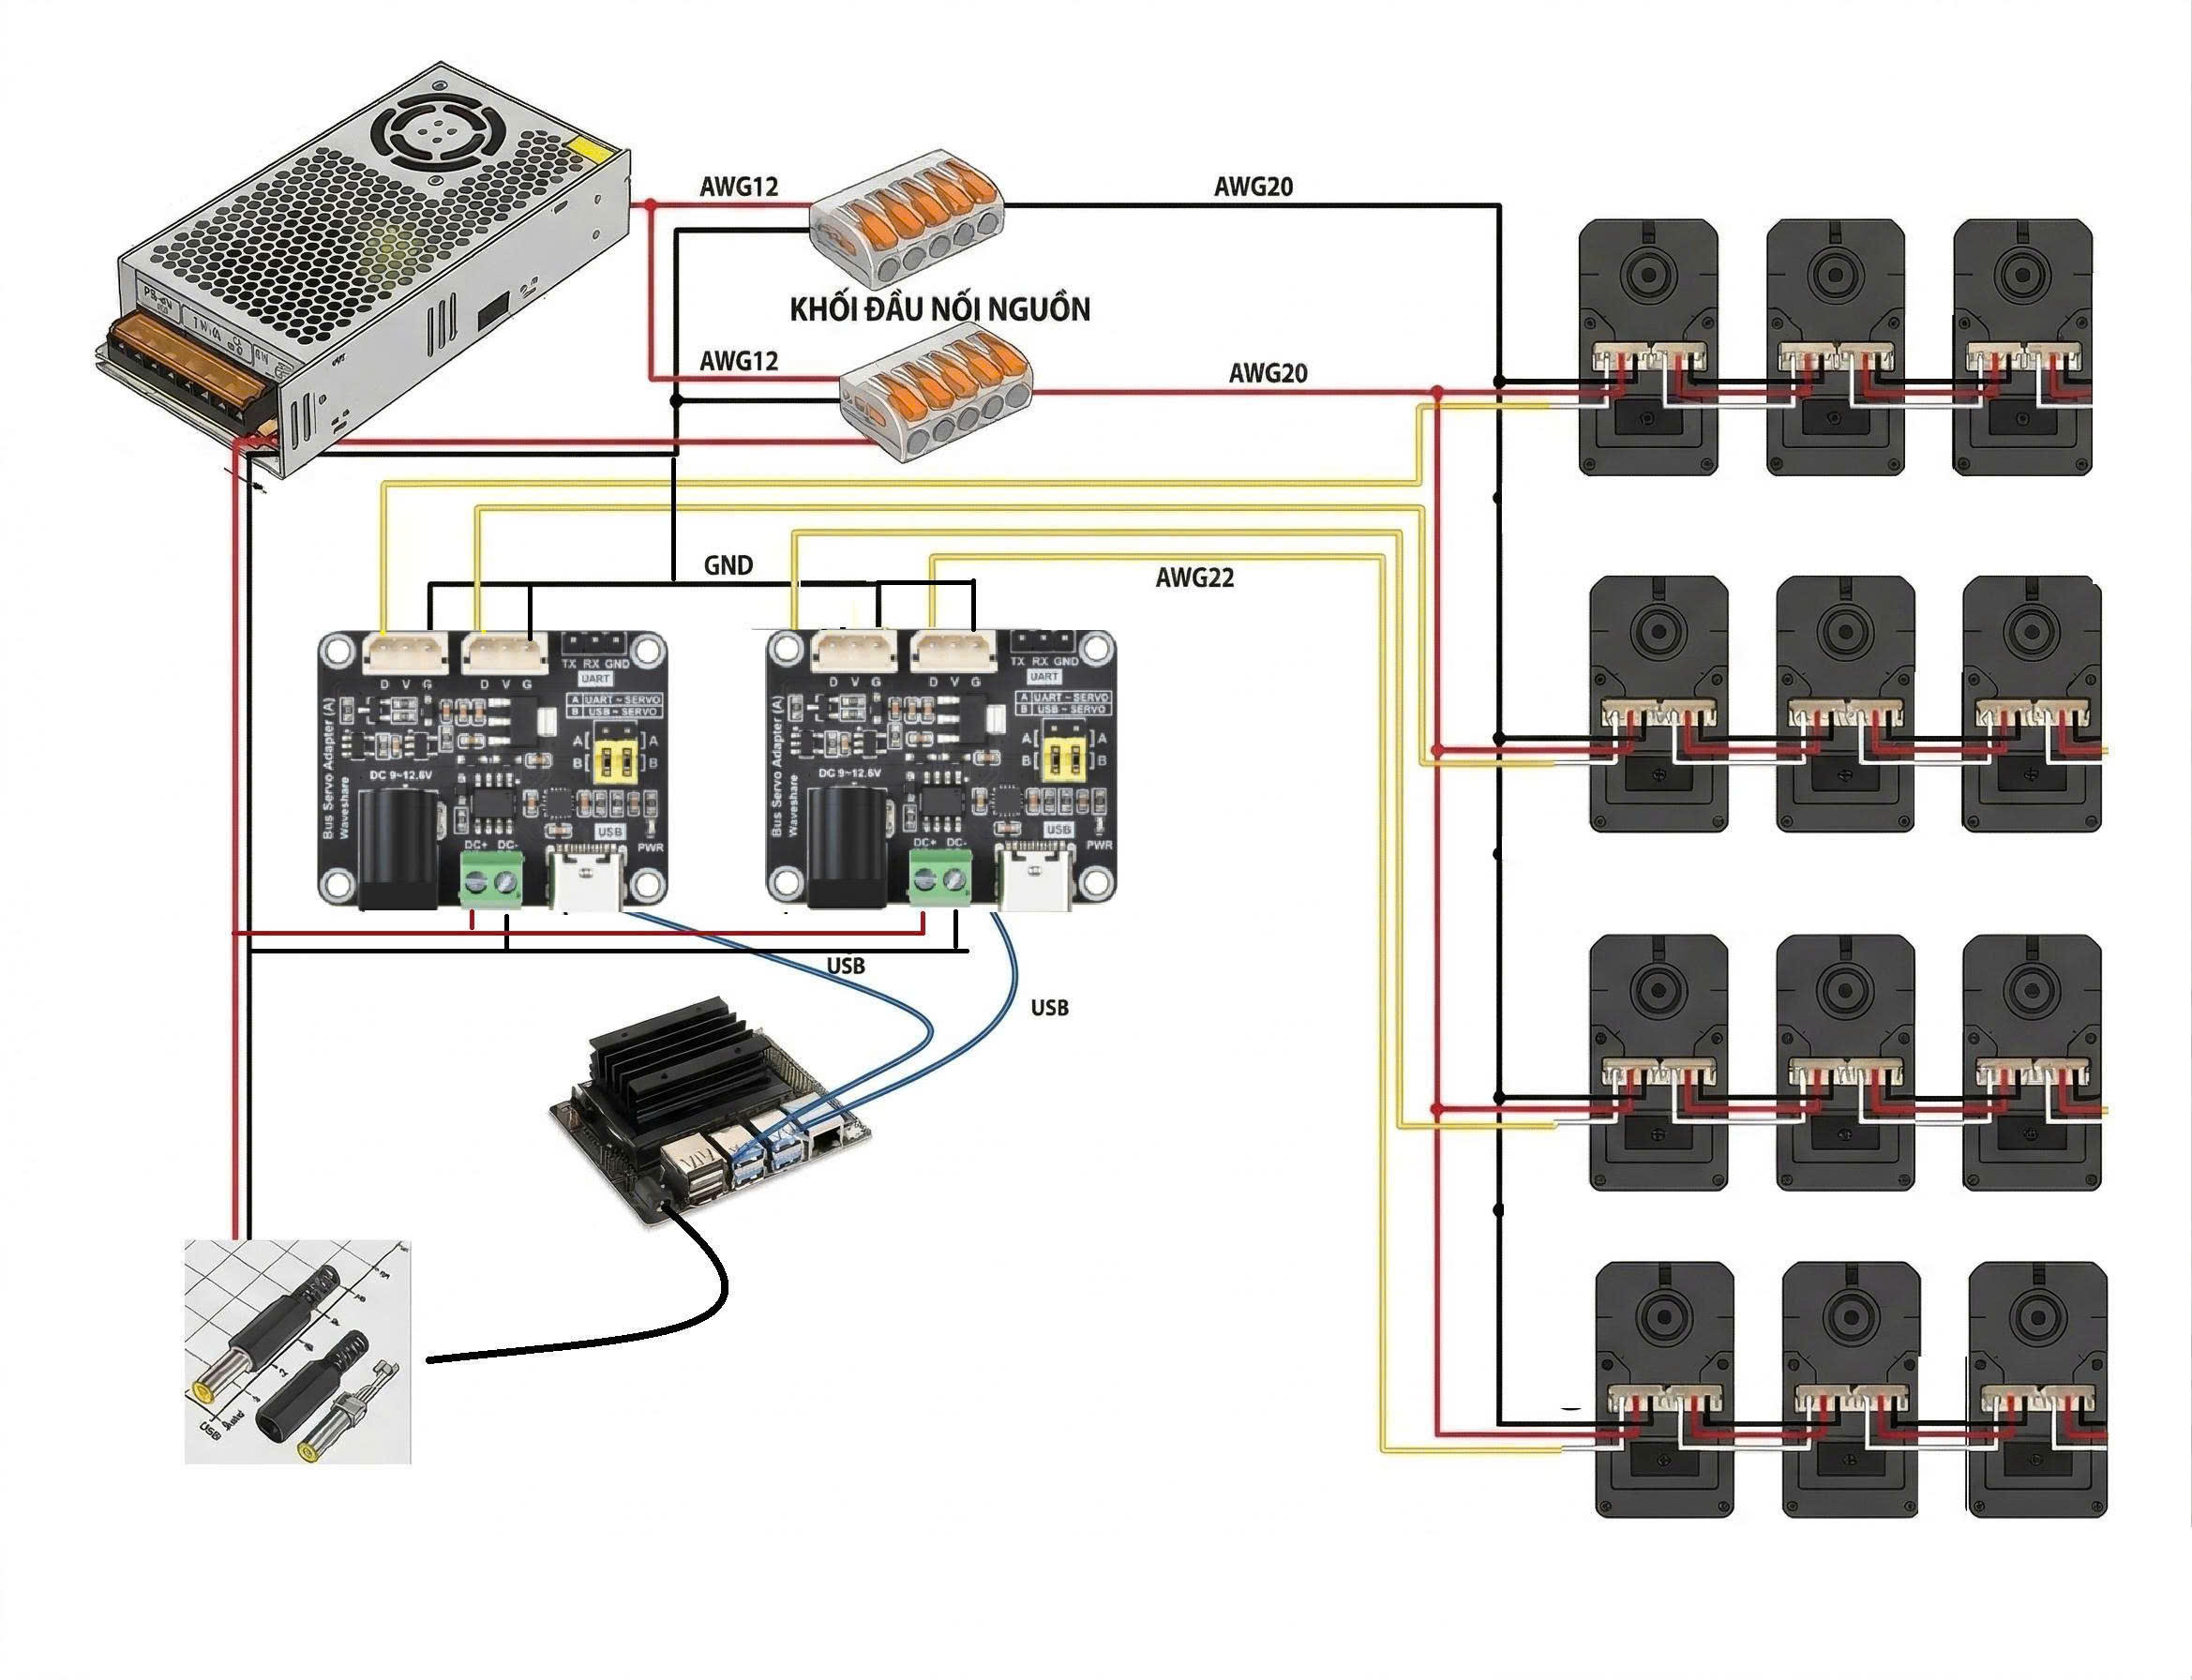
\includegraphics[width=1.0\textwidth]{hardware/system_wiring_diagram.jpg} 
    \caption{Sơ đồ phân phối điện áp và tín hiệu tổng thể của robot}
    \label{fig44}
\end{figure}

Dựa trên thông số kỹ thuật (Datasheet) của các loại dây lõi đồng, nhóm đã đưa ra thiết kế đi dây như sau:

Đối với trục nguồn chính (từ nguồn tổ ong đến khối đấu nối), cáp AWG 12 được sử dụng. Loại cáp này đóng vai trò truyền tải toàn bộ dòng điện từ nguồn xung 12~V - 40~A đến các khối chia nguồn trung tâm. Với đường kính lõi khoảng 2.05 mm, tiết diện 3.31 mm$^2$, khả năng chịu dòng trong không khí mở đạt 30A - 40A cùng điện trở cực thấp (khoảng 5.2 $\Omega$/km), dây AWG 12 hoàn toàn đáp ứng được dòng xả tức thời 32.4A của 12 servo mà không sinh nhiệt hay gây sụt áp đáng kể.

Đối với nhánh nguồn phụ (từ khối đấu nối đến servo đầu tiên), cáp AWG 20 được áp dụng nhằm cấp nguồn trực tiếp cho chuỗi 3 servo của mỗi chân. Với đường kính lõi 0.81 mm và tiết diện 0.52 mm$^2$, loại dây này chịu được dòng định mức khoảng 5A (tối đa 11A). Vì mỗi nhánh 3 servo ST3215 có dòng khởi động tổng cộng khoảng 8.1A, dây AWG 20 cung cấp sự cân bằng hoàn hảo giữa khả năng tải dòng an toàn và độ mềm dẻo cần thiết để luồn lách linh hoạt qua các khớp cơ khí.

Cuối cùng, đối với bus tín hiệu truyền thông (từ Adapter đến servo), cáp AWG 22 được lựa chọn để truyền tín hiệu UART (Data) và nối chung chân Mass (GND) nhằm đồng bộ điện áp logic. Với đường kính lõi 0.64 mm, do đặc thù đường truyền dữ liệu chỉ tiêu thụ dòng điện vài mA, việc sử dụng dây AWG 22 giúp cáp tín hiệu trở nên nhỏ gọn, hạn chế nhiễu chéo, thuận tiện cho việc bấm cos và đi dây nối tiếp (daisy-chain) qua từng servo mà hoàn toàn không cản trở chuyển động của các khớp chân.

Việc thiết kế phân nhánh nguồn thông qua Terminal Block kết hợp với việc tính toán và lựa chọn đúng cỡ dây AWG từ datasheet giúp giải quyết triệt để vấn đề sụt áp trên đường dây (Voltage Drop), đảm bảo 12 động cơ ở cuối chuỗi vẫn nhận đủ điện áp 12~V để sinh ra mô-men xoắn tối đa.

\section{Các Giao thức Truyền thông của Hệ thống}

Hệ thống điều khiển sử dụng hai giao thức truyền thông chính: I2C (tần số 400 kHz) để thu thập dữ liệu tư thế từ cảm biến IMU BNO055 và UART (tốc độ 1 Mbps) để điều khiển 12 cơ cấu chấp hành ST3215 thông qua mạch Bus Servo Adapter (A). Việc sử dụng UART bán song công với tốc độ truyền tải cao trên hai bus vật lý riêng biệt giúp đảm bảo hệ thống duy trì được thời gian phản hồi theo yêu cầu của vòng lặp điều khiển thời gian thực.

\subsection{Phân tích thời gian truyền thông UART}

Việc phân tích thời gian truyền thông trên bus UART là cần thiết để đảm bảo tốc độ cập nhật lệnh servo đáp ứng yêu cầu thời gian thực của vòng lặp điều khiển. Với baudrate 1 Mbps và giao thức bán song công (half-duplex), mỗi giao dịch bao gồm:

Trong một giao dịch hoàn chỉnh, gói lệnh ghi (Write) bao gồm tổng cộng 10 byte, được cấu thành từ header (2 byte), ID servo (1 byte), chiều dài (1 byte), lệnh (1 byte), dữ liệu vị trí và tốc độ (4 byte), cùng checksum (1 byte). Tương ứng, gói phản hồi (Response) gồm tổng cộng 8 byte, phân bổ cho header (2 byte), ID servo (1 byte), chiều dài (1 byte), mã lỗi (1 byte), dữ liệu (2 byte) và checksum (1 byte).

Với cấu hình 8N1 (8 bit dữ liệu, không parity, 1 stop bit), mỗi byte cần 10 bit truyền. Thời gian cho một giao dịch hoàn chỉnh (ghi + đọc) với một servo:

\begin{equation}
    t_{servo} = \frac{(10 + 8) \times 10}{10^6} = 180 \; \mu\text{s}
\end{equation}

Mỗi bus driver quản lý 6 servo, thời gian tổng cho một frame lệnh:

\begin{equation}
    t_{bus} = 6 \times t_{servo} = 6 \times 180 = 1080 \; \mu\text{s} \approx 1{,}1 \text{ ms}
\end{equation}

Hai bus hoạt động song song trên hai cổng USB riêng biệt, nên tổng thời gian truyền thông cho 12 servo vẫn xấp xỉ $1{,}1$ ms --- nhỏ hơn nhiều so với chu kỳ điều khiển $\Delta T = 7$ ms. Điều này xác nhận băng thông truyền thông đủ cho vận hành thời gian thực.

\subsection{Ánh xạ ID servo và phân bổ driver}

Bảng~\ref{tab:servo_mapping} trình bày cấu hình ánh xạ ID servo và phân bổ cho hai driver UART.

\begin{table}[H]
\centering
\caption{Ánh xạ ID servo theo driver và chân robot}
\label{tab:servo_mapping}
\renewcommand{\arraystretch}{1.3}
\begin{tabular}{|l|c|c|c|c|}
\hline
\textbf{Chân} & \textbf{Driver} & \textbf{Hip Roll} & \textbf{Hip Pitch} & \textbf{Knee} \\ \hline
Left-Front (LF) & A & ID 7 & ID 8 & ID 9 \\ \hline
Right-Behind (RB) & A & ID 10 & ID 11 & ID 12 \\ \hline
Right-Front (RF) & B & ID 1 & ID 2 & ID 3 \\ \hline
Left-Behind (LB) & B & ID 4 & ID 5 & ID 6 \\ \hline
\end{tabular}
\end{table}

Chiến lược phân bổ ghép hai chân \textit{chéo nhau} trên cùng một driver (LF+RB trên Driver A, RF+LB trên Driver B) có ý nghĩa quan trọng: trong dáng đi Trot, hai chân chéo luôn ở cùng pha (vung chân hoặc chống chân). Khi một cặp chéo đang ở pha vung chân (cần cập nhật vị trí nhanh), cặp còn lại ở pha chống chân (ít thay đổi), giúp cân bằng tải truyền thông giữa hai bus.


% !TeX root = ../thesis.tex
\chapter{THIẾT KẾ VÀ THỰC HIỆN PHẦN MỀM}

\section{Kiến trúc phần mềm ROS 2}

\subsection{Tổng quan kiến trúc node}

Hệ thống phần mềm được triển khai trên nền tảng ROS~2 Humble \cite{ros2docs}, sử dụng kiến trúc xử lý phân tán gồm hai node tính toán được phân vùng theo chức năng:

\begin{itemize}
    \item \textbf{Gait Generator Node (Node Điều khiển dáng đi):} Quản lý toàn bộ quá trình tính toán quỹ đạo tuần hoàn, giải bài toán động học nghịch và gửi lệnh điều khiển đến các cơ cấu chấp hành qua bus nối tiếp. Node này được tổ chức thành các phân hệ chức năng: Phân hệ tạo dáng đi (quản lý trạng thái), Phân hệ động học nghịch (IK solver), Phân hệ nội suy quỹ đạo (đa thức bậc 5) và Phân hệ giao tiếp phần cứng (UART).
    
    \item \textbf{Balance Controller Node (Node Cân bằng tư thế):} Xử lý bất đồng bộ việc thu thập dữ liệu quán tính tần số cao, xử lý tín hiệu đa giai đoạn và tính toán bù PID. Node này hoạt động như một tiến trình độc lập để đảm bảo chu kỳ điều khiển không bị gián đoạn.
\end{itemize}

\subsection{Kiến trúc phân tầng và phương pháp thiết kế Sim-to-Real}

Điểm nổi bật trong kiến trúc phần mềm ROS~2 của hệ thống là khả năng chuyển đổi liền mạch giữa môi trường mô phỏng (Gazebo) và phần cứng thực tế (Hardware) mà không yêu cầu chỉnh sửa thuật toán điều khiển cốt lõi (tư tưởng Sim-to-Real). Để đạt được điều này, hệ thống được thiết kế theo cấu trúc phân tầng (layered architecture), tách biệt rõ ràng các khối xử lý thuật toán khỏi các giao diện điều khiển thiết bị vật lý.

Trong môi trường mô phỏng (Hình~\ref{fig:ros2_arch_sim}), kiến trúc phần mềm được chia thành hai phân vùng chính:
\begin{itemize}
    \item \textbf{Tầng điều khiển phần mềm (ROS 2 Software Control):} Chứa hai node thuật toán cốt lõi là \texttt{Balance Controller Node} và \texttt{Gait Generator Node}. Hai node này giao tiếp nội bộ với nhau qua các topic \texttt{/posture/correction} để chia sẻ tín hiệu bù thăng bằng.
    \item \textbf{Tầng mô phỏng (Gazebo Simulation Environment):} Hoạt động như một robot ảo, trong đó \texttt{imu\_plugin} đóng vai trò xuất bản dữ liệu quaternion thay cho cảm biến thật, còn \texttt{controller\_manager} đóng vai trò quản lý mô-men và góc khớp ảo dựa trên lệnh \texttt{/effort\_controller} từ bộ tạo dáng đi.
\end{itemize}

\begin{figure}[H]
    \centering
    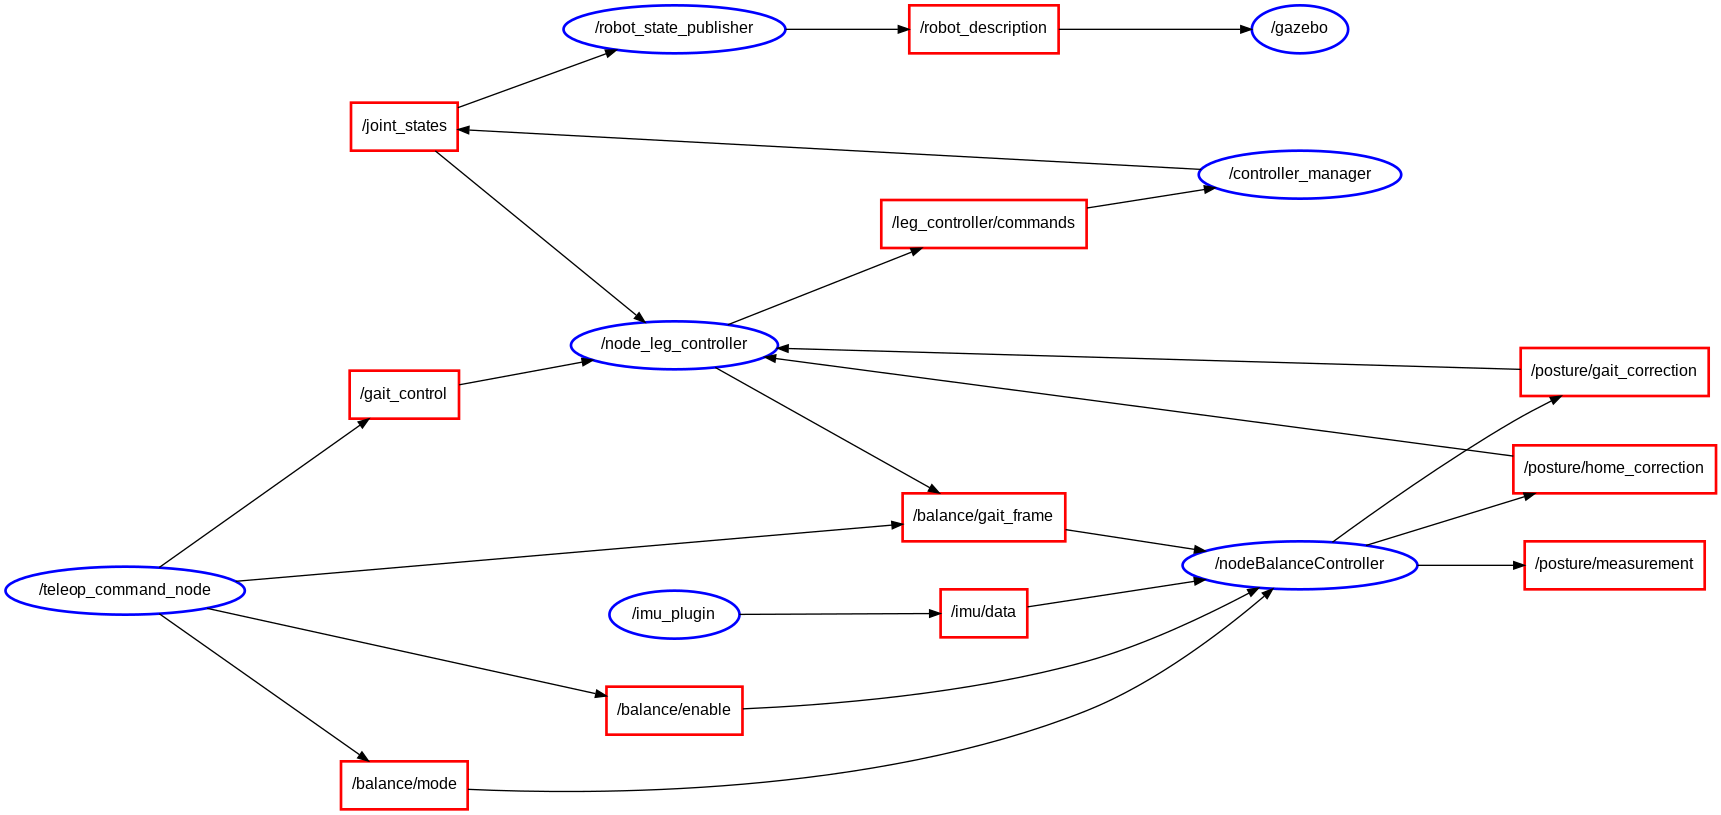
\includegraphics[width=0.95\textwidth]{architecture/simulation_rqt_graph.png}
    \caption{Sơ đồ kiến trúc khối ROS~2 của hệ thống trong môi trường mô phỏng (Gazebo)}
    \label{fig:ros2_arch_sim}
\end{figure}

Ngược lại, khi chuyển sang vận hành trên robot thực tế (Hình~\ref{fig:ros2_arch_hw}), hệ thống thay thế toàn bộ Tầng mô phỏng bằng hai tầng vật lý chuyên dụng, trong khi vẫn \textbf{giữ nguyên} nguyên bản Tầng thuật toán cốt lõi (Tầng 1). Kiến trúc thực tế bao gồm ba tầng rõ rệt:
\begin{itemize}
    \item \textbf{Tầng 1 -- ROS 2 Core Algorithms:} Chứa các node giải quyết bài toán động học, nội suy quỹ đạo và điều khiển PID (tái sử dụng 100\% mã nguồn từ mô phỏng).
    \item \textbf{Tầng 2 -- Hardware Interface Drivers:} Đóng vai trò cầu nối, bao gồm \texttt{imu\_sensor\_node} để chuyển đổi luồng I2C thành message ROS~2 tiêu chuẩn, cùng với \texttt{serial\_driver\_a} và \texttt{serial\_driver\_b} làm nhiệm vụ dịch các mảng góc khớp mục tiêu thành gói tin bus servo thông qua thư viện SCServo SDK.
    \item \textbf{Tầng 3 -- Physical Hardware:} Gồm các linh kiện điện tử vật lý là cảm biến BNO055 IMU và chuỗi 12 động cơ ST3215 Servo giao tiếp theo chuẩn UART/RS485.
\end{itemize}

Sự phân tách ba tầng này giúp hệ thống đạt độ tin cậy vận hành rất cao, đồng thời cho phép việc bảo trì hay nâng cấp cảm biến, động cơ trong tương lai chỉ gói gọn ở việc thay đổi driver ở Tầng 2 mà không ảnh hưởng tới chất lượng thuật toán.

\begin{figure}[H]
    \centering
    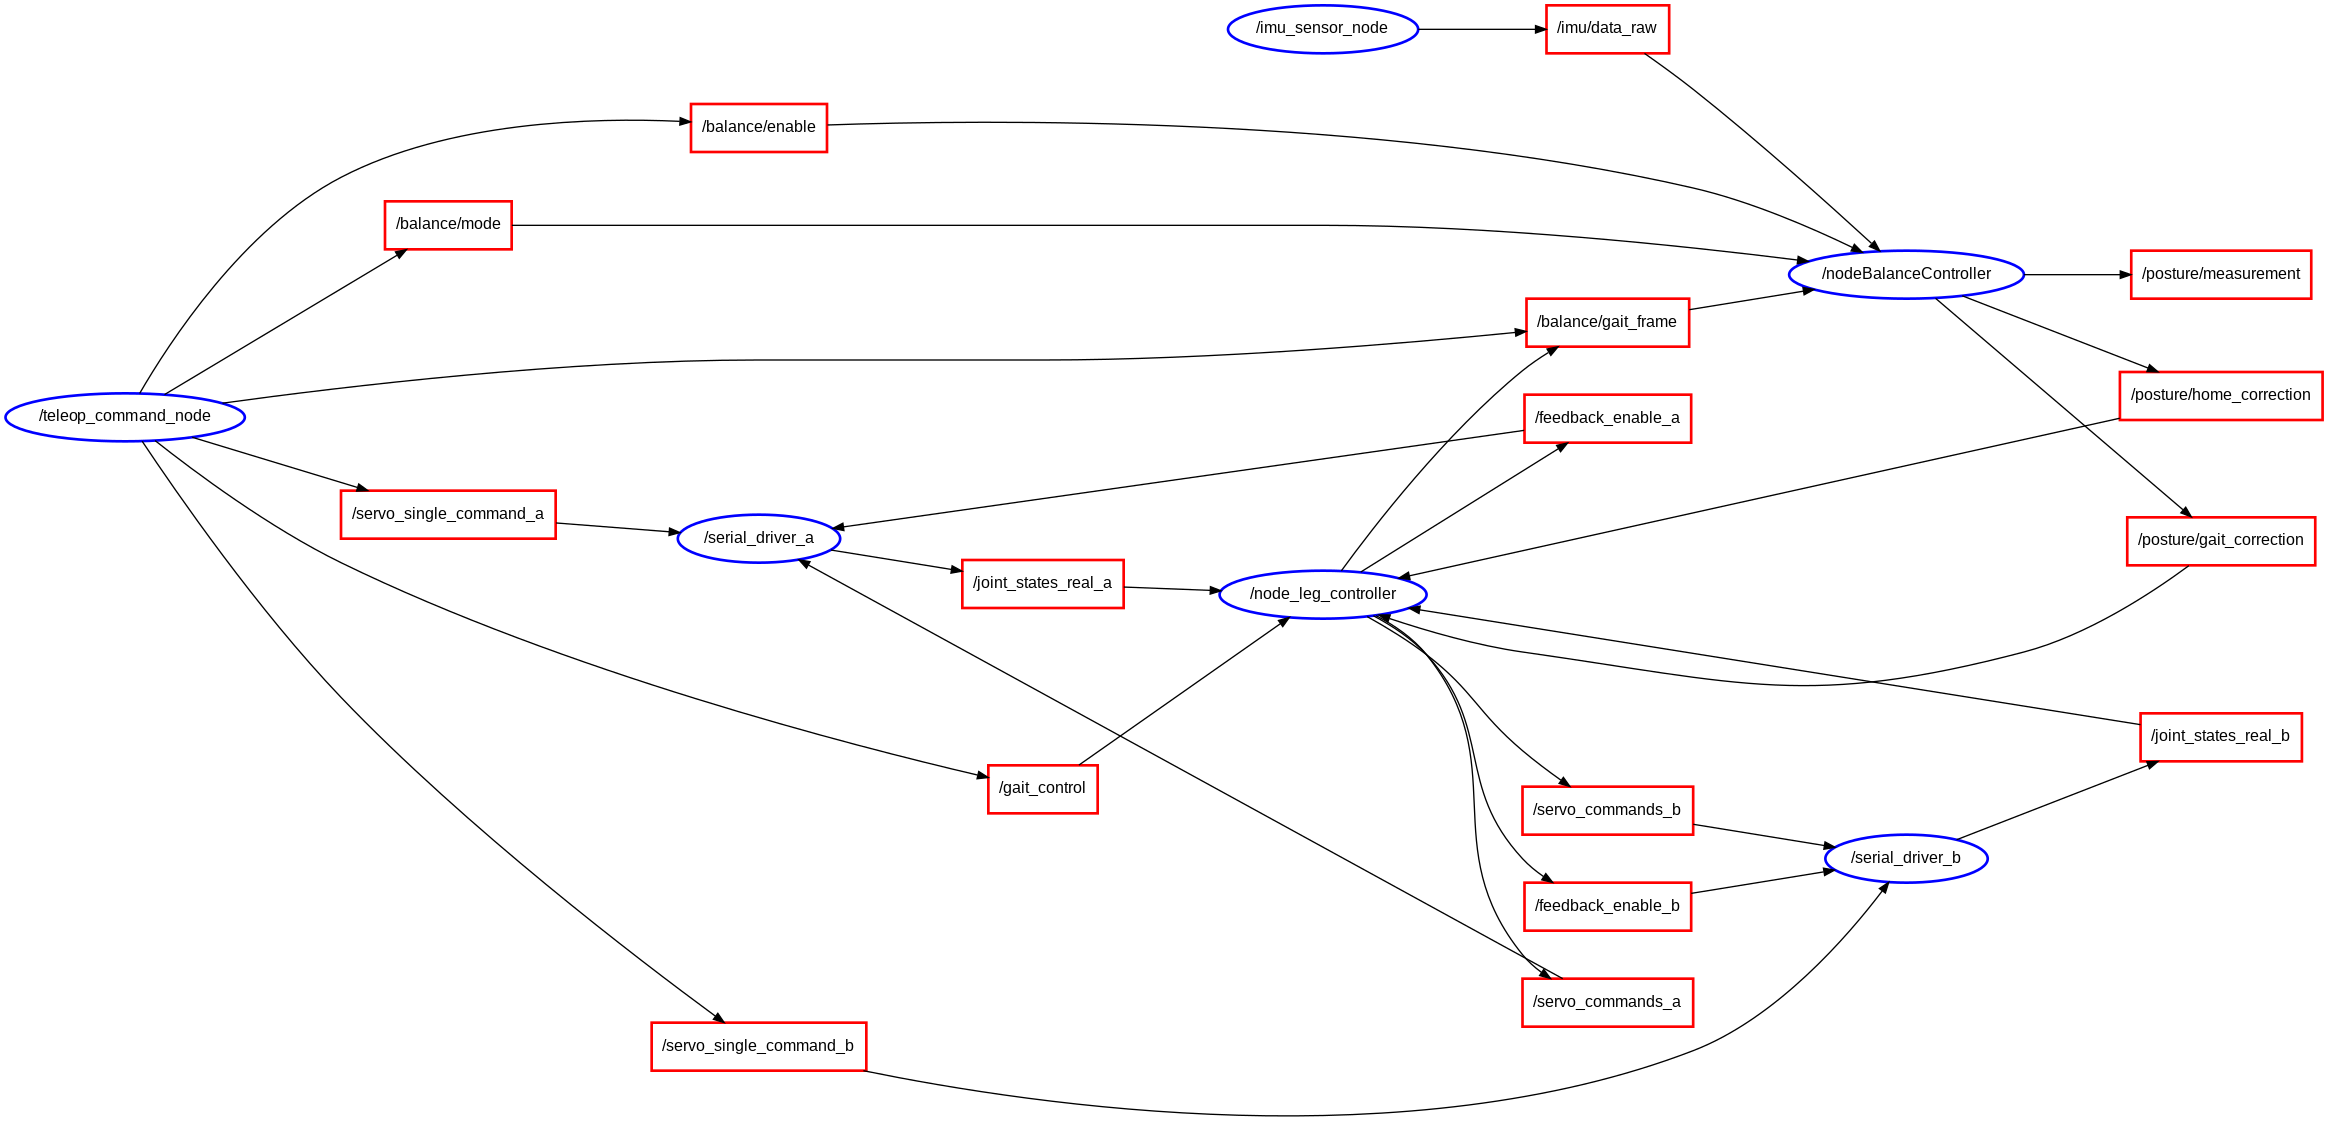
\includegraphics[width=0.95\textwidth]{architecture/hardware_rqt_graph.png}
    \caption{Sơ đồ kiến trúc ROS~2 phân tầng của hệ thống trên phần cứng thực tế}
    \label{fig:ros2_arch_hw}
\end{figure}

\subsection{Các trạng thái vận hành}

Hệ thống quản lý hai trạng thái vận hành rời rạc thông qua cổng logic boolean:

\begin{itemize}
    \item \textbf{HOME:} Cấu hình tĩnh không có vector tịnh tiến tuần hoàn. Bộ điều khiển tính toán các điều chỉnh đồng nhất trong không gian khớp, ánh xạ cứng đến tư thế nghỉ. Sai lệch góc cơ sở được chuyển đổi tỷ lệ thành các bù mô-men đối kháng nhằm hiệu chỉnh tư thế liên tục. Một khoảng trễ khởi động $T_{delay}$ giây có thể cấu hình giúp ngăn hiệu chỉnh sớm trong giai đoạn quá độ khởi tạo hệ thống.
    
    \item \textbf{GAIT:} Trạng thái động kích hoạt khi có lệnh tịnh tiến mặt phẳng. Robot thực hiện quỹ đạo đa thức tuần hoàn sử dụng các mảng dịch pha khả cấu hình để tạo dáng đi trot (với LF, RB: 0 và LB, RF: 0,5), walk (với LF: 0, RB: 0,25, RF: 0,5, LB: 0,75) và các dáng đi khác. Các hiệu chỉnh không gian từ phản hồi quán tính chỉ được áp dụng cho chân ở pha chống, trong khi chân ở pha bay duy trì bù bằng không để đảm bảo khoảng trống sải bước.
\end{itemize}

\subsection{Cấu trúc các ROS 2 packages}

Toàn bộ hệ thống phần mềm được tổ chức thành 6 packages ROS~2:

\begin{table}[H]
\centering
\caption{Cấu trúc các ROS 2 packages trong hệ thống}
\label{tab:ros2_packages}
\renewcommand{\arraystretch}{1.3}
\begin{tabular}{|p{0.25\linewidth}|p{0.12\linewidth}|p{0.49\linewidth}|}
\hline
\textbf{Package} & \textbf{Ngôn ngữ} & \textbf{Chức năng} \\ \hline
\texttt{leg\_controller} & Python & Tạo dáng đi, IK solver, quy hoạch quỹ đạo, giao tiếp servo \\ \hline
\texttt{balance\_controller} & Python & Thu thập IMU, xử lý tín hiệu, PID cân bằng, chẩn đoán \\ \hline
\texttt{serial\_driver} & C++ & Driver giao tiếp với bus servo ST3215 (thư viện SCServo) \\ \hline
\texttt{simulation} & Python & Mô hình URDF, cấu hình Gazebo, RViz, launch mô phỏng \\ \hline
\texttt{launch\_main} & CMake & Launch files cho hệ thống thực \\ \hline
\end{tabular}
\end{table}

\subsection{Chi tiết các module phần mềm}

\textbf{Phân hệ điều khiển trung tâm (Gait Generator)} là phân hệ cốt lõi của hệ thống, quản lý máy trạng thái (state machine) điều khiển toàn bộ vòng đời vận hành của robot. Phân hệ này thực hiện các chức năng:

\begin{itemize}
    \item \textbf{Quản lý trạng thái:} Robot chuyển đổi giữa các trạng thái: INIT (khởi tạo) $\rightarrow$ ZERO (khởi tạo tư thế đứng) $\rightarrow$ TROT/WALK/PUSHUP/SWAY (dáng đi) $\rightarrow$ ROBOTOFF (tắt an toàn). Mỗi trạng thái có chu trình cập nhật độc lập để xử lý logic trong một khung thời gian điều khiển (frame).
    \item \textbf{Tạo quỹ đạo:} Gọi thuật toán nội suy quỹ đạo để tạo quỹ đạo hình chữ D cho mỗi chân, sau đó giải phương trình động học nghịch (IK) để chuyển đổi từ tọa độ Đề-các sang không gian góc khớp.
    \item \textbf{Áp dụng hiệu chỉnh IMU:} Nhận tín hiệu bù từ Balance Controller qua hai topic \texttt{/posture/}\allowbreak\texttt{home\_correction} và \texttt{/posture/}\allowbreak\texttt{gait\_correction}, áp dụng vào góc khớp (HOME) hoặc tọa độ bàn chân (GAIT).
    \item \textbf{Xuất lệnh servo:} Gửi góc điều khiển đến phân hệ giao tiếp phần cứng để chuyển đổi từ góc khớp phân tích sang góc vật lý của servo và truyền qua giao thức UART.
\end{itemize}

\textbf{Phân hệ giao tiếp phần cứng (Serial Publish)} đảm nhận việc chuyển đổi giữa hai chế độ vận hành (mô phỏng và phần cứng thực) thông qua cấu hình môi trường:

\begin{itemize}
    \item \textbf{Chế độ mô phỏng:} Xuất bản lệnh mô-men (effort) lên topic \texttt{/effort\_controller/commands} để điều khiển robot trong Gazebo thông qua plugin \texttt{gazebo\_ros2\_control}.
    \item \textbf{Chế độ phần cứng:} Chuyển đổi góc từ động học nghịch sang độ phân giải của servo bằng các hàm ánh xạ riêng biệt cho từng chân (xử lý ngược chiều quay do lắp đặt đối xứng), sau đó đóng gói dữ liệu và xuất bản lên các topic giao tiếp serial.
\end{itemize}

\subsection{Bảng giao tiếp topic ROS~2}

Bảng~\ref{tab:ros2_topics} liệt kê các topic chính trong hệ thống, phân loại theo chức năng.

\begin{table}[H]
\centering
\caption{Các topic ROS~2 chính trong hệ thống}
\label{tab:ros2_topics}
\renewcommand{\arraystretch}{1.3}
\begin{tabular}{|p{0.32\linewidth}|p{0.12\linewidth}|p{0.42\linewidth}|}
\hline
\textbf{Topic} & \textbf{Kiểu dữ liệu} & \textbf{Mô tả} \\ \hline
\texttt{/imu/data} & Imu & Dữ liệu quaternion từ BNO055 \\ \hline
\texttt{/balance/enable} & Bool & Bật/tắt bộ PID cân bằng \\ \hline
\texttt{/balance/mode} & String & Chuyển chế độ HOME/GAIT \\ \hline
\texttt{/balance/gait\_frame} & Int32 & Chỉ số frame dáng đi hiện tại \\ \hline
\texttt{/posture/home\_correction} & Vector3 & Tín hiệu bù PID chế độ HOME \\ \hline
\texttt{/posture/gait\_correction} & Vector3 & Tín hiệu bù PID chế độ GAIT \\ \hline
\texttt{/posture/measurement} & Vector3 & Góc roll/pitch đã lọc \\ \hline
\texttt{/servo\_commands\_a} & Float64[] & Lệnh góc cho Driver A (6 servo) \\ \hline
\texttt{/servo\_commands\_b} & Float64[] & Lệnh góc cho Driver B (6 servo) \\ \hline
\end{tabular}
\end{table}

\subsection{Cơ chế chẩn đoán thời gian thực}

Hệ thống tích hợp cơ chế chẩn đoán (diagnostics) cho phép giám sát trực tiếp các biến nội bộ của bộ điều khiển PID trong thời gian thực thông qua công cụ PlotJuggler. Mỗi giai đoạn trong pipeline PID (đo lường $\rightarrow$ sai lệch $\rightarrow$ P/I/D $\rightarrow$ bão hòa $\rightarrow$ lọc) đều có topic chẩn đoán riêng, cho phép:

\begin{itemize}
    \item Quan sát trực tiếp từng thành phần P, I, D và tổng PID
    \item Phát hiện hiện tượng windup hoặc bão hòa đầu ra
    \item So sánh tín hiệu đo (measurement) với điểm đặt (setpoint) để đánh giá chất lượng bám
    \item Ghi lại dữ liệu dưới dạng file CSV để phân tích offline
\end{itemize}

Tổng cộng, hệ thống xuất bản 22 topic chẩn đoán cho chế độ HOME (9 tín hiệu $\times$ 2 trục + 4 tín hiệu áp dụng) và 18 topic cho chế độ GAIT (9 tín hiệu $\times$ 2 trục), cung cấp khả năng quan sát toàn diện luồng xử lý điều khiển.

\section{Quy trình Homing và Calibrate}

\subsection{Calibrate servo}

Trước khi vận hành, mỗi servo cần được calibrate để đảm bảo góc $0^\circ$ cơ học trùng với góc $0^\circ$ trong phần mềm. Quy trình calibrate bao gồm:

\begin{enumerate}
    \item Đặt tất cả chân robot ở tư thế tham chiếu (chân duỗi thẳng, vuông góc với thân).
    \item Đọc vị trí feedback của từng servo qua thư viện SCServo SDK.
    \item Ghi giá trị offset ($\Delta_{calib}$) --- sai lệch giữa vị trí thực tế và vị trí lý thuyết tại góc $0^\circ$.
    \item Lưu offset vào tập tin cấu hình của hệ thống, áp dụng tự động trong các lần khởi chạy tiếp theo.
\end{enumerate}

\subsection{Quy trình Homing}

Quy trình khởi tạo tư thế đứng (homing) được thực hiện tự động mỗi khi robot khởi động:

\begin{enumerate}
    \item \textbf{Đọc vị trí hiện tại:} Lấy giá trị góc feedback từ tất cả 12 servo ($\theta_{current,i}$).
    \item \textbf{Tính tư thế đích:} Giải IK cho tư thế đứng chuẩn, tạo ra bộ góc đích $\theta_{target,i} = (0^\circ, 0^\circ, 90^\circ)$ cho mỗi chân.
    \item \textbf{Nội suy tuyến tính:} Trong $N_{homing} = 200$ frame, mỗi góc được nội suy tuyến tính:
    \begin{equation}
        \theta_i(k) = \theta_{current,i} + \frac{k}{N_{homing}} (\theta_{target,i} - \theta_{current,i}), \quad k = 0, 1, \ldots, N_{homing}
    \end{equation}
    \item \textbf{Gửi lệnh:} Tại mỗi frame, gửi bộ 12 góc đã nội suy đến servo qua UART.
\end{enumerate}

Phương pháp nội suy tuyến tính đảm bảo chuyển động mượt mà từ bất kỳ vị trí khởi đầu nào, tránh hiện tượng giật hoặc va đập. Tổng thời gian khởi tạo: $200 \times 3 = 600$ ms $= 0{,}6$ giây.


% !TeX root = ../thesis.tex
\chapter{KẾT QUẢ THỰC HIỆN}

% !TeX root = ../thesis.tex

%

\section{Giới thiệu}
Chương này trình bày kết quả mô phỏng hệ thống robot bốn chân sử dụng nền tảng ROS~2 Humble \cite{ros2docs} kết hợp với trình mô phỏng Gazebo Classic \cite{gazebo}. Trước khi triển khai trên mô phỏng phức tạp Gazebo, bộ điều khiển PID được mô hình hóa và kiểm chứng sơ bộ trên môi trường Matlab/Simulink để xác minh tính đáp ứng động học. Mục tiêu của toàn bộ quá trình mô phỏng là xác minh tính đúng đắn của các thuật toán lập kế hoạch quỹ đạo, động học nghịch (Inverse Kinematics), và bộ điều khiển PID trước khi triển khai trên robot thực. Toàn bộ kết quả được trình bày thông qua các hình minh họa, bao gồm cấu hình mô phỏng, trực quan hóa quá trình hoạt động, đánh giá quỹ đạo bàn chân, biên dạng góc khớp và hiệu năng bộ điều khiển PID.

Nội dung chương được tổ chức như sau: Mục~5.2 trình bày mô phỏng và đánh giá bộ điều khiển bằng Matlab/Simulink; Mục~5.3 trình bày cấu hình chi tiết của môi trường mô phỏng Gazebo; Mục~5.4 đánh giá hiệu năng bộ điều khiển PID nâng cao cùng với quỹ đạo sinh ra trên mô phỏng; và Mục~5.5 trình bày kết quả thực nghiệm trên phần cứng cùng phân tích so sánh sim-to-real.

\section{Mô phỏng và đánh giá bộ điều khiển bằng Matlab/Simulink}

Để kiểm chứng bộ điều khiển PID trước khi đưa vào hệ thống thực tế hoặc môi trường mô phỏng Gazebo, toàn bộ hệ thống động học và điều khiển của robot được mô hình hóa trên môi trường Matlab/Simulink. Hệ thống được tổ chức thành một vòng lặp kín (Closed-loop) hoàn chỉnh như thể hiện trong Hình~\ref{fig:simulink_block_diagram}. Chu trình điều khiển bao gồm 3 khối chức năng chính: khối đối tượng vật lý (Quadruped Robot) cung cấp phản hồi trạng thái, khối điều khiển (PID Controller) tính toán tín hiệu bù, và khối thực thi (Execution) chuyển đổi lệnh bù thành góc khớp.

\begin{figure}[H]
    \centering
    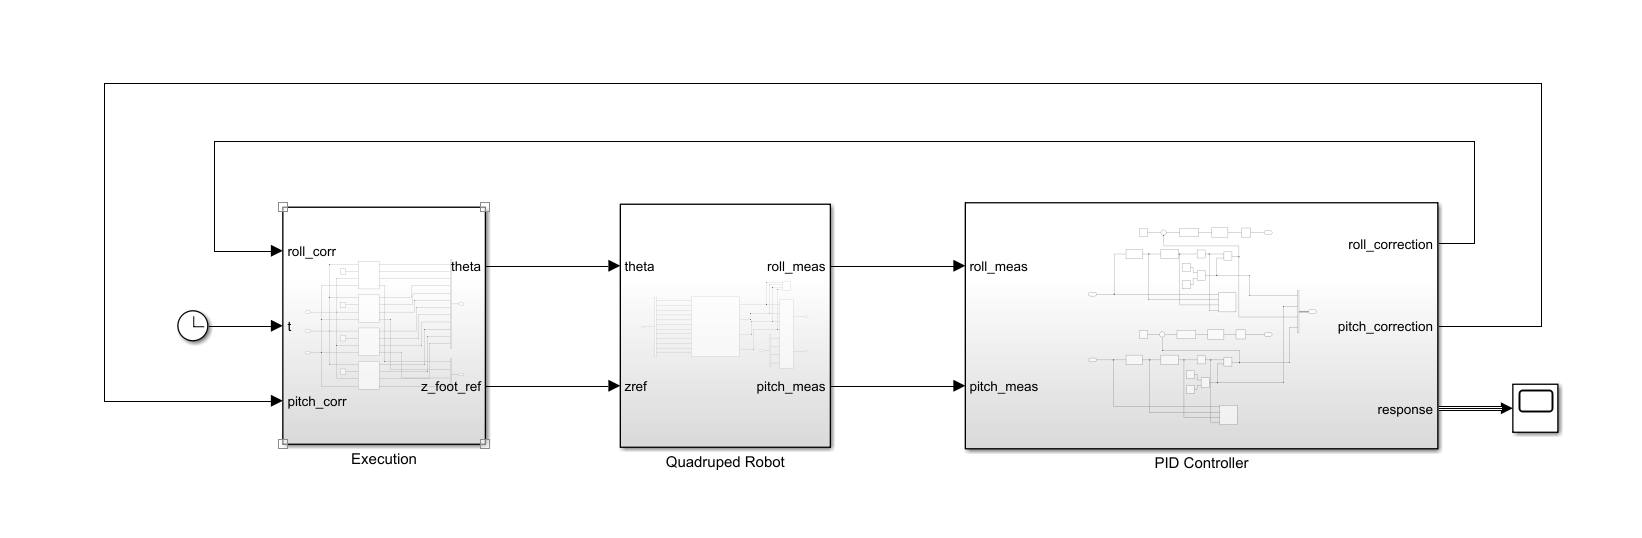
\includegraphics[width=\textwidth]{img_matlab/fig1-PID-controller.png}
    \caption{Sơ đồ khối tổng thể vòng lặp kín điều khiển tư thế robot}
    \label{fig:simulink_block_diagram}
\end{figure}

\subsection{Mô hình toán học đối tượng (Quadruped Robot)}
Khối Quadruped Robot (Hình~\ref{fig:simulink_quadruped_robot}) đóng vai trò là "môi trường vật lý ảo" của hệ thống. Đầu vào của khối này là bộ $12$ lệnh góc khớp $\theta$ sinh ra từ bộ điều khiển. Đầu ra là các giá trị cao độ bàn chân (\texttt{z\_out}) và phản hồi cảm biến IMU (\texttt{roll\_meas}, \texttt{pitch\_meas}). Sơ đồ này mô phỏng quy trình thu thập trạng thái cơ cấu chấp hành để tái tạo lại tư thế định hướng của thân robot.

\begin{figure}[H]
    \centering
    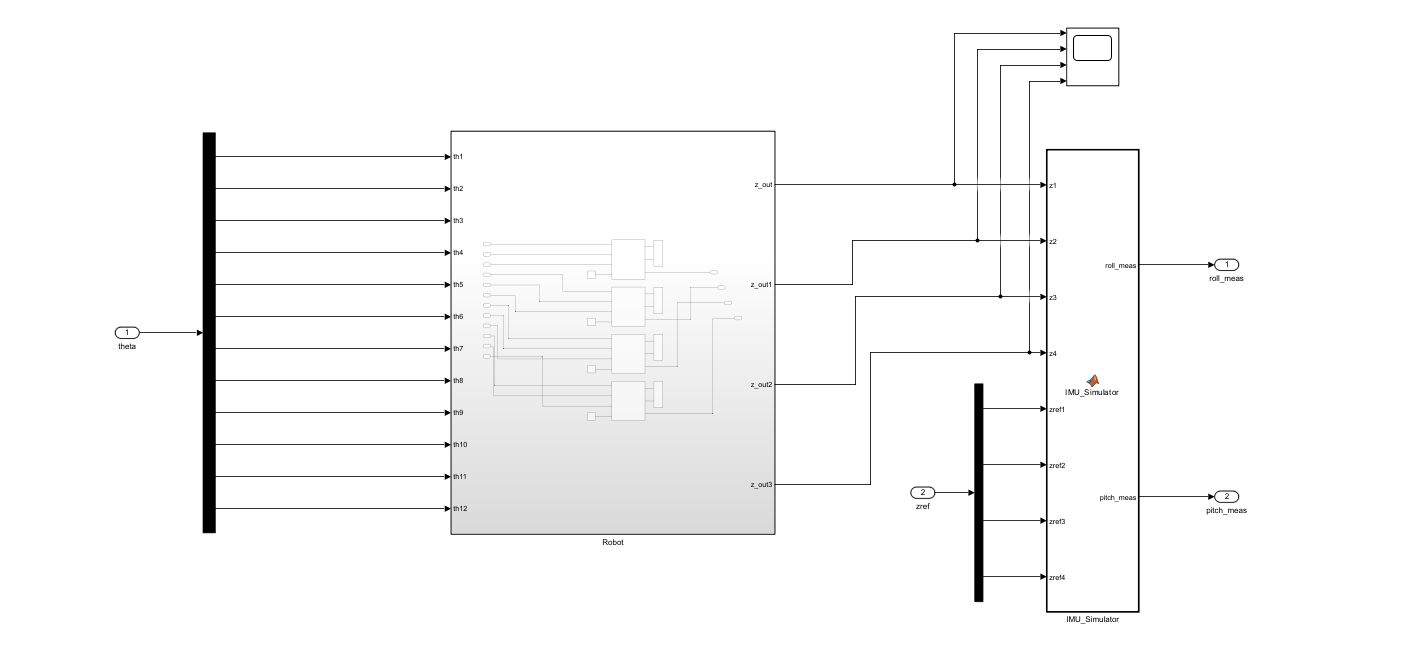
\includegraphics[width=0.8\textwidth]{img_matlab/fig3-quadruped-robot.png}
    \caption{Cấu trúc khối đối tượng mô phỏng phản hồi trạng thái (Quadruped Robot)}
    \label{fig:simulink_quadruped_robot}
\end{figure}

Sâu bên trong khối Robot, Hình~\ref{fig:simulink_forward_kinematics} phơi bày cấu trúc mô hình hóa động học của robot. Tại đây, hệ thống sử dụng 4 khối \texttt{Universal\_FK} chạy song song để giải phương trình động học thuận cho 4 chân. Từ các góc khớp $\theta_{1,2,3}$ của từng chân, mô hình ánh xạ ra tọa độ không gian thực $(x, y, z)$ của bàn chân đối với hệ quy chiếu thân robot. Giá trị \texttt{z\_out} thu được chính là cơ sở toán học để mô phỏng trạng thái nghiêng thân và xác định độ cân bằng của toàn hệ thống trong không gian 3D.

\begin{figure}[H]
    \centering
    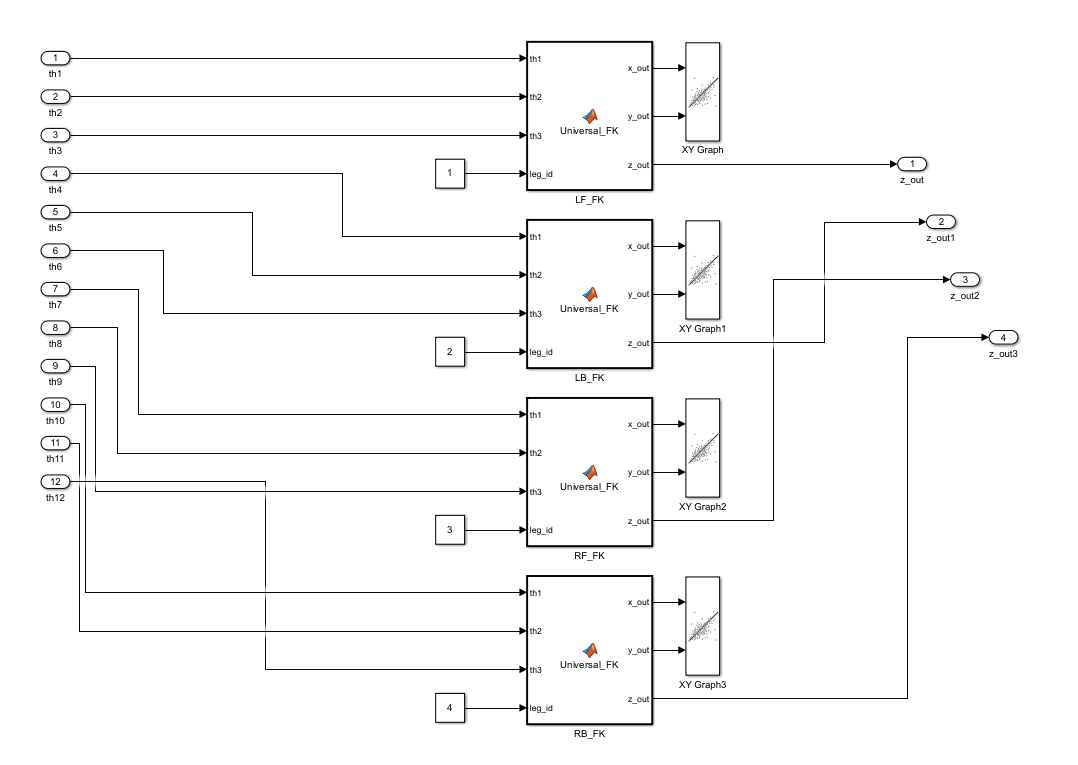
\includegraphics[width=\textwidth]{img_matlab/fig4-mo-hinh-hoa-robot.png}
    \caption{Cấu trúc mô hình hóa động học robot (dựa trên phương trình Động học thuận)}
    \label{fig:simulink_forward_kinematics}
\end{figure}

\subsection{Thiết kế bộ điều khiển PID và tiền xử lý tín hiệu}
Tín hiệu phản hồi từ mô hình Robot tiếp tục được đưa vào khối PID Controller (Hình~\ref{fig:pid_simulink_detail}). Khối này không chỉ thực hiện tính toán P-I-D đơn thuần mà còn bao hàm toàn bộ chuỗi tiền xử lý tín hiệu (Signal Processing Pipeline) để giải quyết hiện tượng nhiễu động học. Tín hiệu thô từ IMU trải qua 3 cấp độ lọc: lọc trung bình trượt hàm mũ (EMA), lọc thông thấp (Avg) để trích xuất sai lệch đường cơ sở, và cuối cùng là đi qua vùng chết (Deadzone). Chỉ những sai lệch đã qua thanh lọc này mới được đưa vào bộ điều khiển Rời rạc \texttt{PID(z)} để xuất ra lệnh bù tư thế (\texttt{roll\_correction}, \texttt{pitch\_correction}), đảm bảo hệ thống phản ứng trơn tru mà không bị đánh lừa bởi dao động bước đi tự nhiên.

\begin{figure}[H]
    \centering
    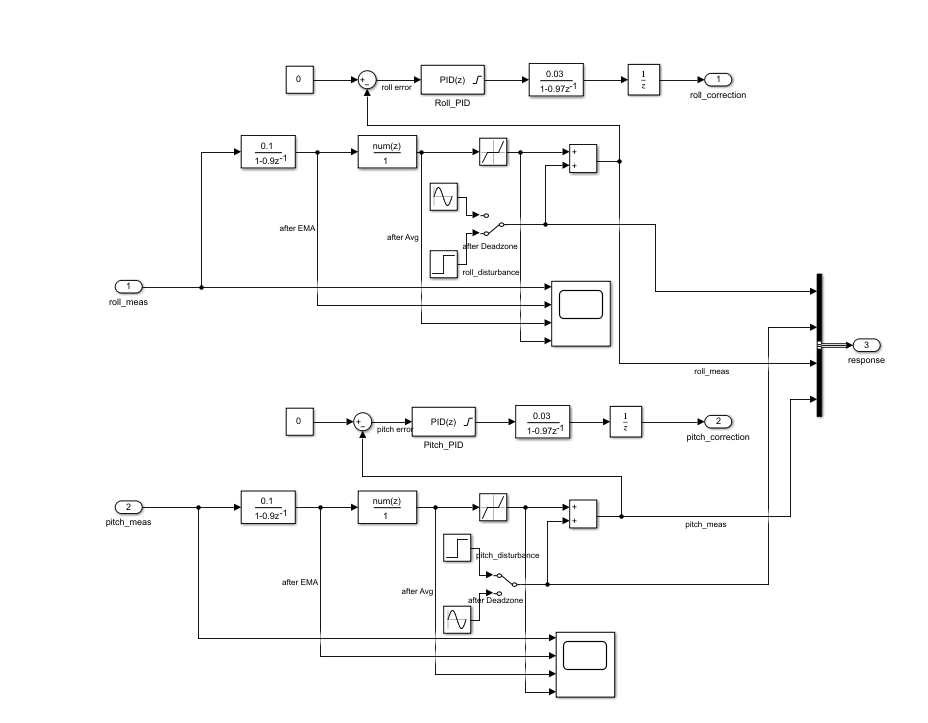
\includegraphics[width=0.8\textwidth]{img_matlab/fig5-PID.png}
    \caption{Chi tiết cấu trúc chuỗi tiền xử lý tín hiệu và khối điều khiển PID rời rạc}
    \label{fig:pid_simulink_detail}
\end{figure}

\subsection{Khối thực thi động học nghịch (Execution)}
Cuối cùng, vòng lặp điều khiển được khép kín tại khối Execution (Hình~\ref{fig:pid_execution_flow}). Nhiệm vụ của khối này là giải quyết bài toán Động học nghịch (Inverse Kinematics). Đầu vào là tín hiệu bù góc Roll và Pitch; đầu ra là tập hợp $12$ quỹ đạo góc khớp \texttt{th1}, \texttt{th2}, \texttt{th3} của 4 chân. Sơ đồ minh họa quá trình ánh xạ ngược: từ yêu cầu duy trì mặt phẳng thăng bằng cho thân robot, khối Execution phân bổ độ dịch chuyển theo trục Z (\texttt{z\_foot\_ref}) xuống từng cơ cấu chân, buộc các động cơ phải tự động gập/duỗi để đáp ứng bù trừ sai lệch theo thời gian thực.

\begin{figure}[H]
    \centering
    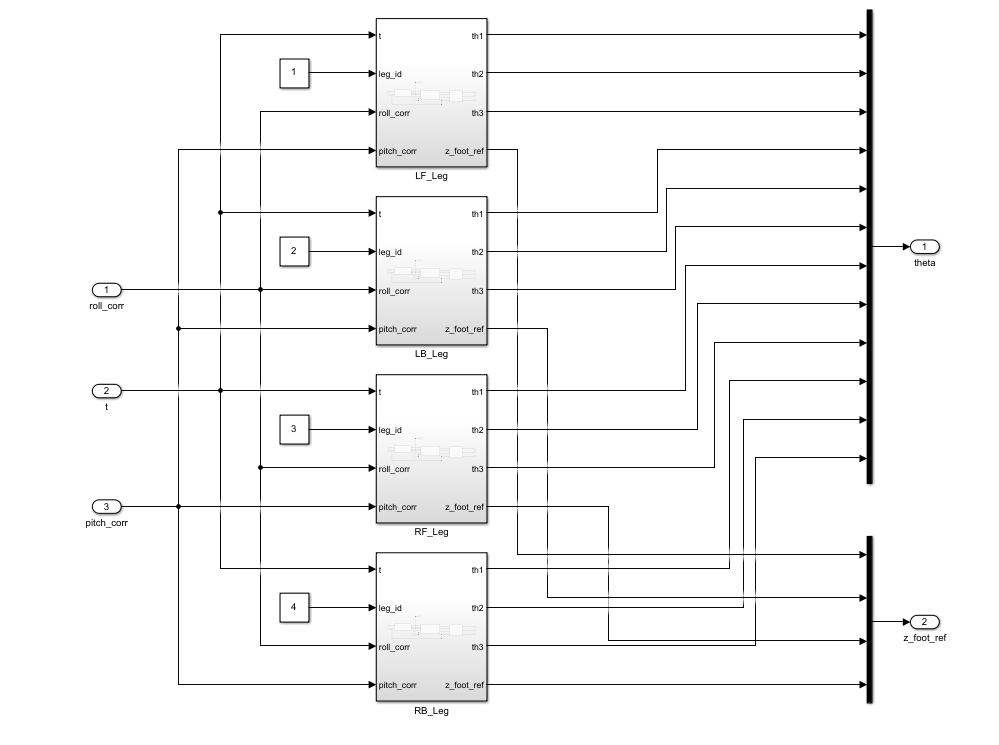
\includegraphics[width=0.8\textwidth]{img_matlab/fig2-execution.png}
    \caption{Cấu trúc khối thực thi giải tích động học nghịch (Inverse Kinematics) cho 4 chân}
    \label{fig:pid_execution_flow}
\end{figure}

\subsection{Kết quả mô phỏng}

\subsubsection*{Quá trình hiệu chỉnh (Tuning) bộ điều khiển PID độc lập cho trục Roll và Pitch}
Trong thực tế, đặc tính động học của robot trên hai trục Roll và Pitch không hoàn toàn giống nhau do sự phân bố khối lượng và khoảng cách các chân (chiều dài cơ sở và chiều rộng cơ sở) khác biệt. Do đó, bộ điều khiển PID được thiết kế để hiệu chỉnh (tuning) độc lập cho từng trục. Quá trình hiệu chỉnh được thực hiện tuần tự từ khâu tỷ lệ (P), vi phân (D) đến tích phân (I) nhằm đạt được sự cân bằng tối ưu giữa tốc độ đáp ứng và độ ổn định.

\textbf{\textit{Hiệu chỉnh bộ điều khiển trục Roll}}

Đầu tiên, khâu tỷ lệ được áp dụng với hệ số $K_p=4$ (Hình~\ref{fig:roll_tuning_p}). Hệ thống đáp ứng nhanh với nhiễu bước $0{,}15$ rad tại $t=3$ s, góc nghiêng giảm mạnh nhưng xảy ra hiện tượng dao động lớn, kéo dài liên tục và tồn tại sai số xác lập rõ rệt quanh mức $0{,}025$ rad.
Tiếp theo, thành phần vi phân được thêm vào ($K_p=4, K_d=1{,}3$) (Hình~\ref{fig:roll_tuning_pd}). Nhờ khả năng dự báo sự thay đổi của khâu D, các dao động được dập tắt nhanh chóng sau khoảng $10$ s, hệ thống trở nên trơn tru hơn nhưng sai số xác lập vẫn chưa được loại bỏ.
Cuối cùng, khâu tích phân được đưa vào ($K_p=4, K_i=1{,}2, K_d=1{,}3$) (Hình~\ref{fig:roll_tuning_pid}). Tại thời điểm này, sai số xác lập bị triệt tiêu hoàn toàn, góc đo được (\texttt{roll\_meas}) từ từ hội tụ chính xác về điểm đặt (setpoint) $0$ rad.

\begin{figure}[H]
    \centering
    \begin{subfigure}[b]{0.48\textwidth}
        \centering
        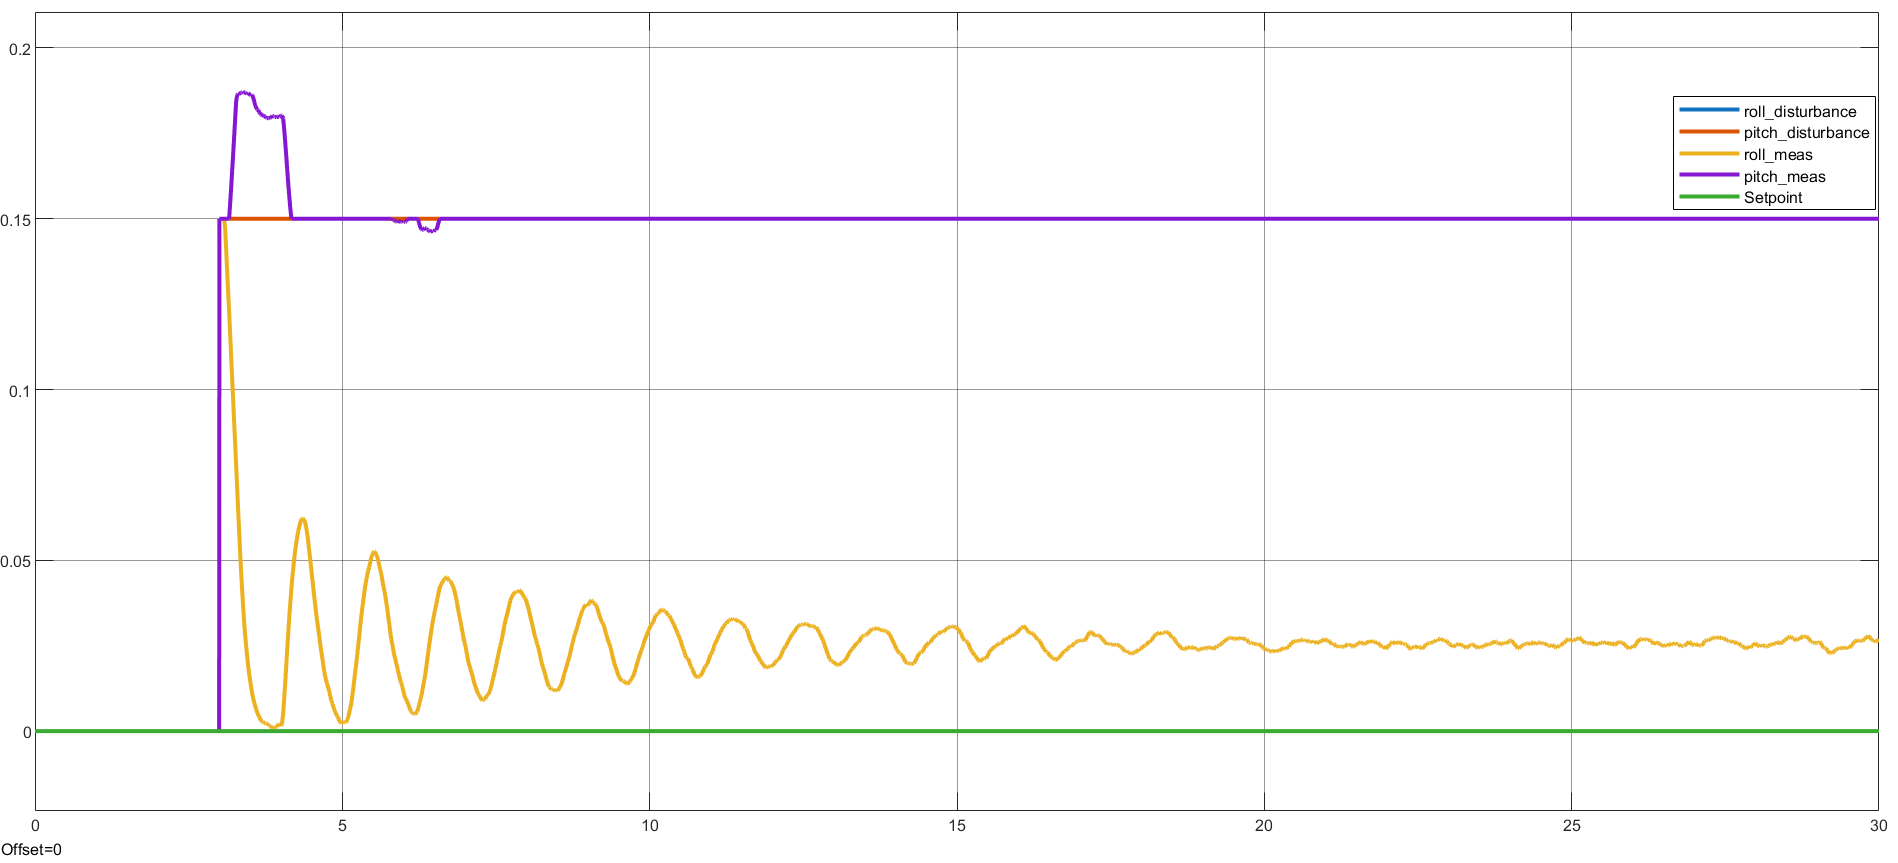
\includegraphics[width=\textwidth]{Images/PID_turning/PID_turning/roll turning Kp=4.png}
        \caption{Chỉ dùng khâu P ($K_p=4$)}
        \label{fig:roll_tuning_p}
    \end{subfigure}
    \hfill
    \begin{subfigure}[b]{0.48\textwidth}
        \centering
        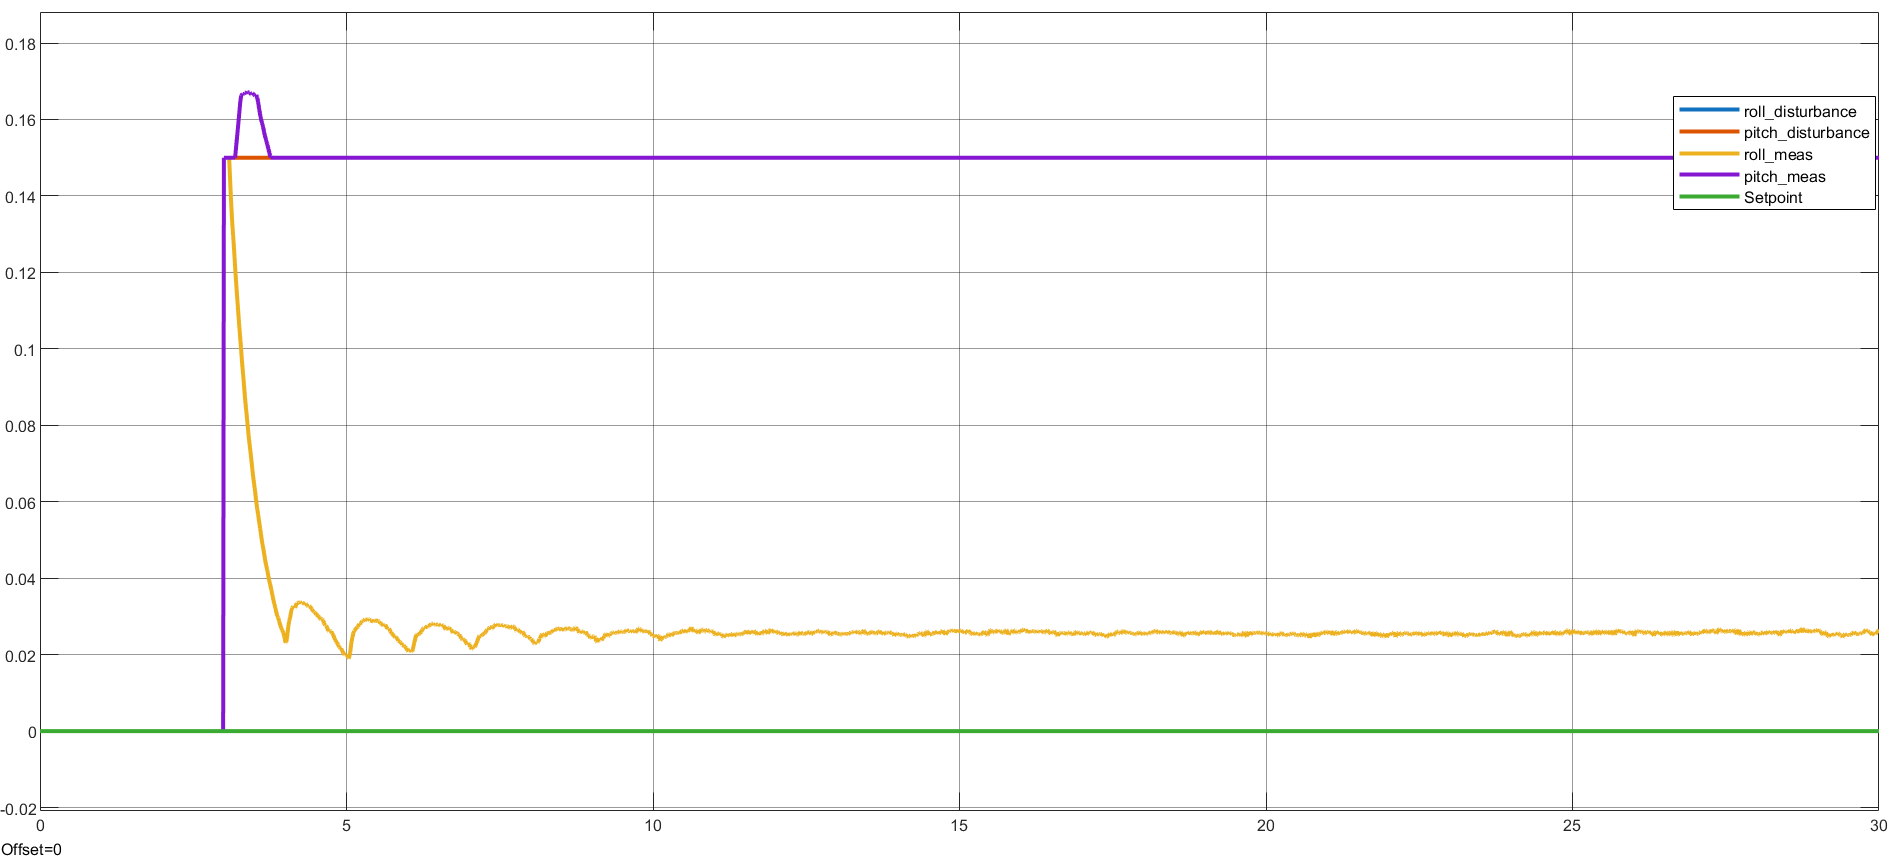
\includegraphics[width=\textwidth]{Images/PID_turning/PID_turning/roll turning Kp=4 Kd=1.3.png}
        \caption{Dùng khâu PD ($K_p=4, K_d=1{,}3$)}
        \label{fig:roll_tuning_pd}
    \end{subfigure}
    
    \vspace{0.2cm}
    \begin{subfigure}[b]{0.6\textwidth}
        \centering
        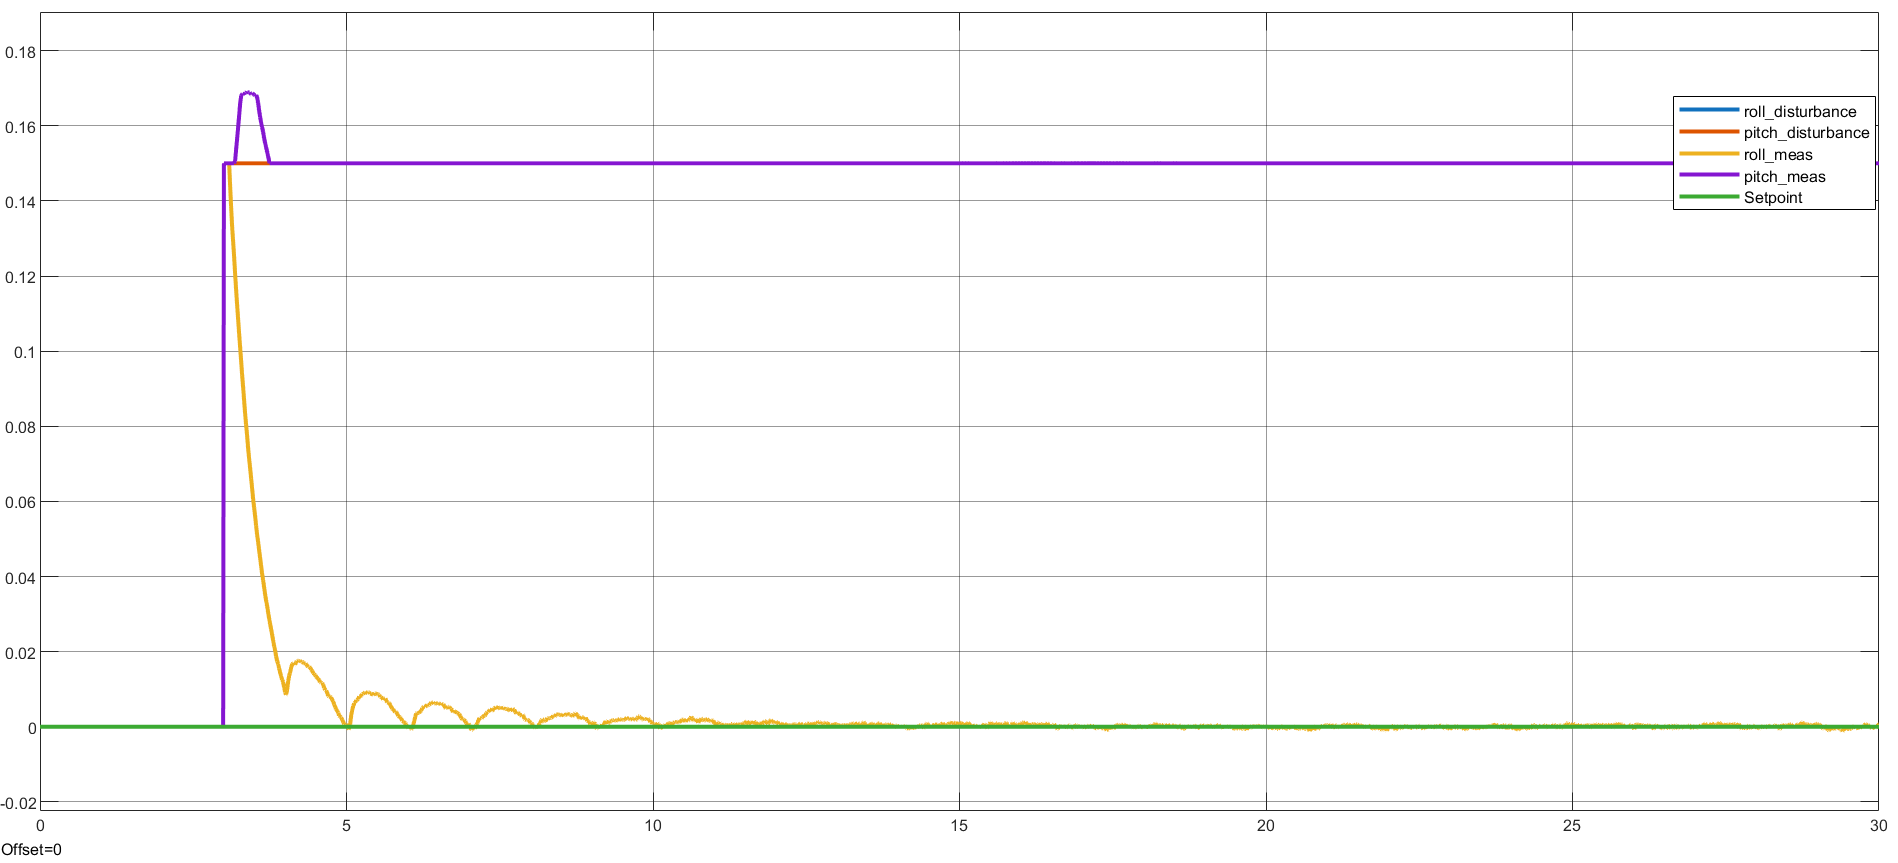
\includegraphics[width=\textwidth]{Images/PID_turning/PID_turning/roll turning Kp=4 Kd=1.3 Ki=1.2.png}
        \caption{Dùng PID hoàn chỉnh ($K_p=4, K_i=1{,}2, K_d=1{,}3$)}
        \label{fig:roll_tuning_pid}
    \end{subfigure}
    \caption{Quá trình hiệu chỉnh các khâu P, D, I cho trục Roll}
    \label{fig:roll_tuning_process}
\end{figure}

\textbf{\textit{Hiệu chỉnh bộ điều khiển trục Pitch}}

Quá trình tương tự được thực hiện cho trục Pitch. Trục này yêu cầu lực bù lớn hơn một chút để chống lại mô-men quán tính theo trục dọc của robot.
Với khâu P ($K_p=5$) (Hình~\ref{fig:pitch_tuning_p}), hệ thống giảm được sai lệch nhưng vẫn dao động. Khi thêm khâu D ($K_p=5, K_d=1{,}3$) (Hình~\ref{fig:pitch_tuning_pd}), dao động được dập tắt nhanh chóng. Cuối cùng, khâu I được bổ sung ($K_p=5, K_i=1{,}6, K_d=1{,}3$) (Hình~\ref{fig:pitch_tuning_pid}) giúp triệt tiêu hoàn toàn sai số xác lập, đưa hệ thống về điểm làm việc tối ưu $0$ rad.

\begin{figure}[H]
    \centering
    \begin{subfigure}[b]{0.48\textwidth}
        \centering
        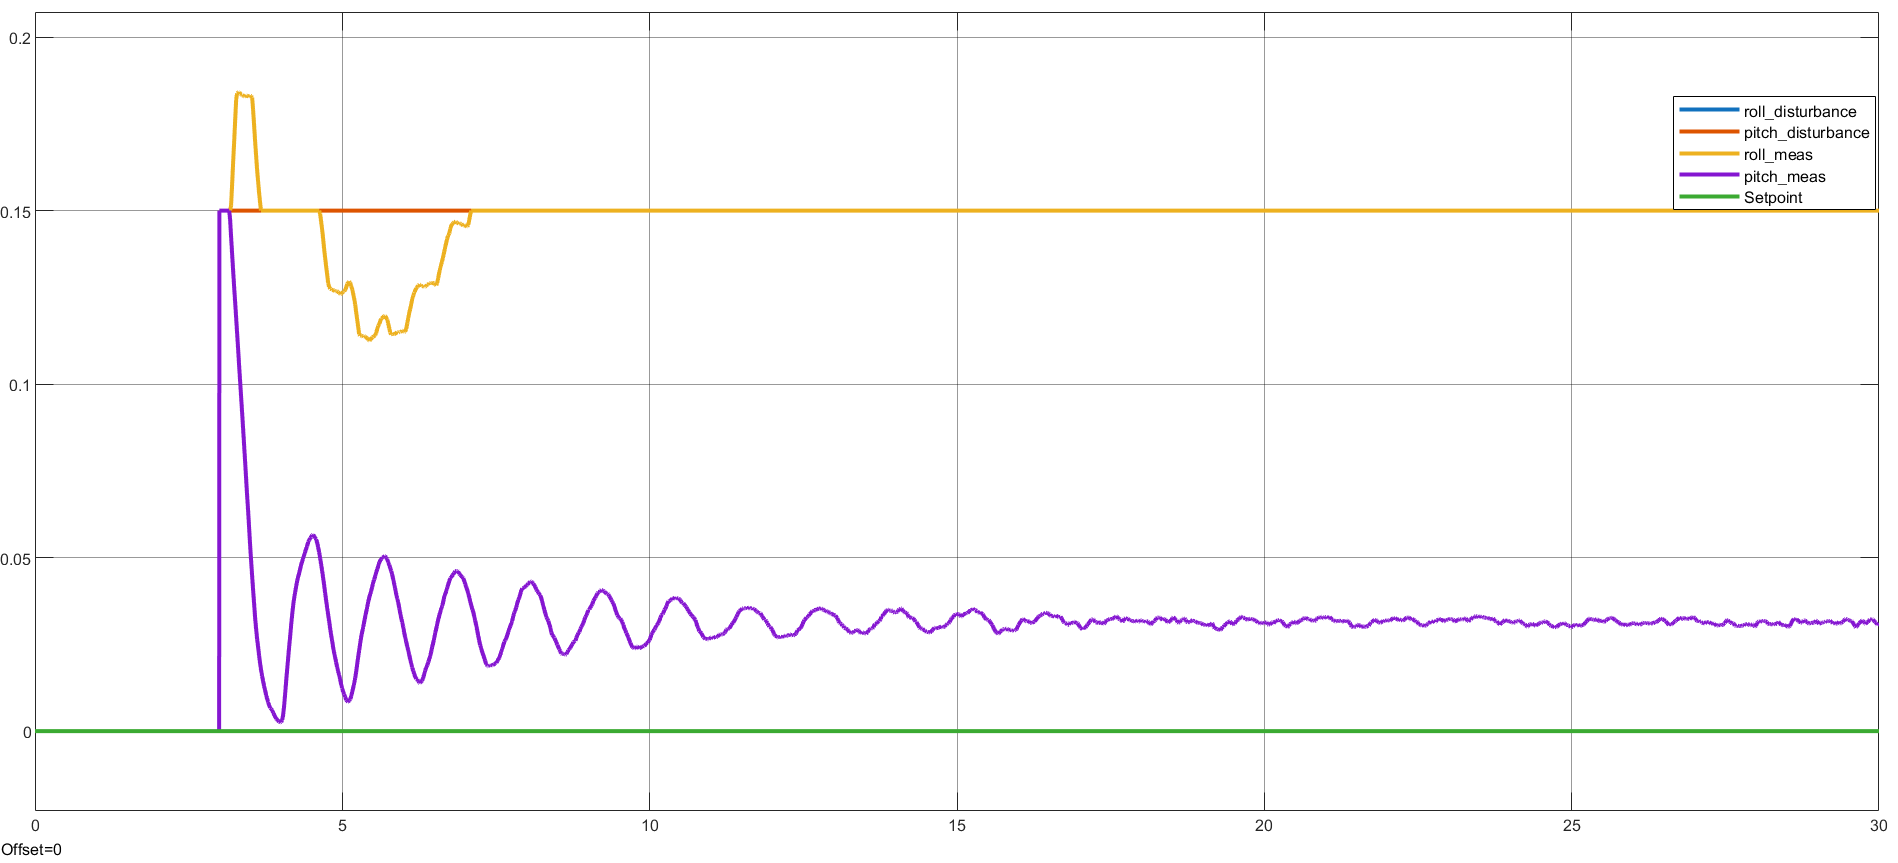
\includegraphics[width=\textwidth]{Images/PID_turning/PID_turning/pitch turning Kp=5.png}
        \caption{Chỉ dùng khâu P ($K_p=5$)}
        \label{fig:pitch_tuning_p}
    \end{subfigure}
    \hfill
    \begin{subfigure}[b]{0.48\textwidth}
        \centering
        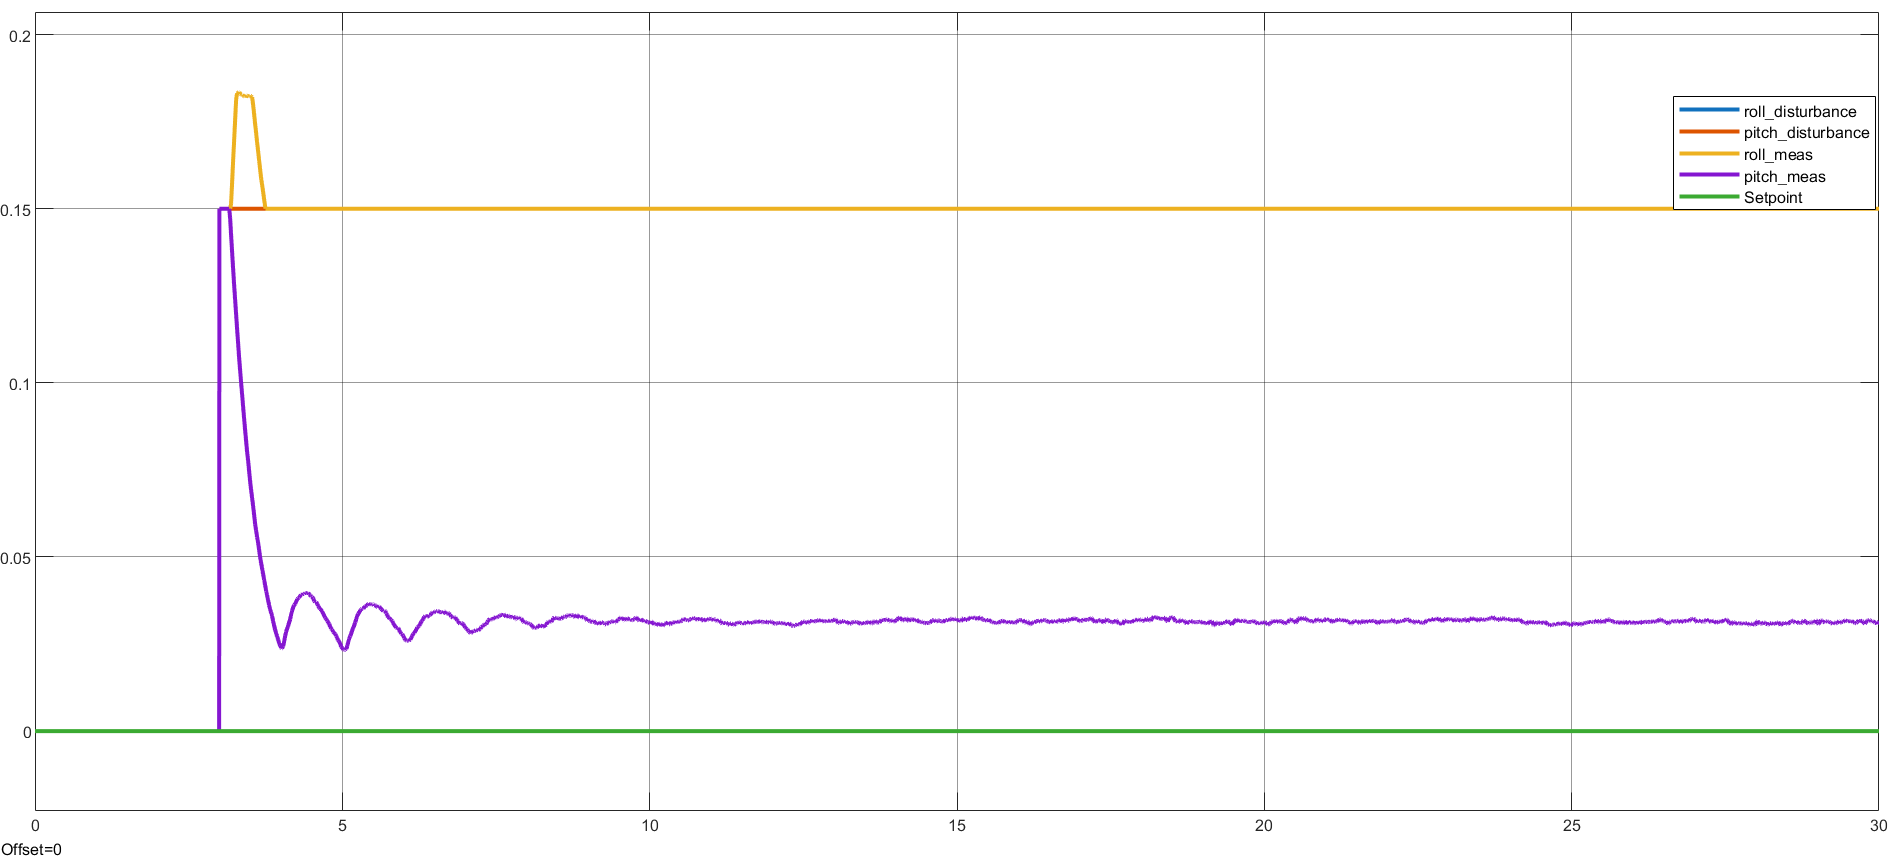
\includegraphics[width=\textwidth]{Images/PID_turning/PID_turning/pitch turning Kp=5 Kd=1.3.png}
        \caption{Dùng khâu PD ($K_p=5, K_d=1{,}3$)}
        \label{fig:pitch_tuning_pd}
    \end{subfigure}
    
    \vspace{0.2cm}
    \begin{subfigure}[b]{0.6\textwidth}
        \centering
        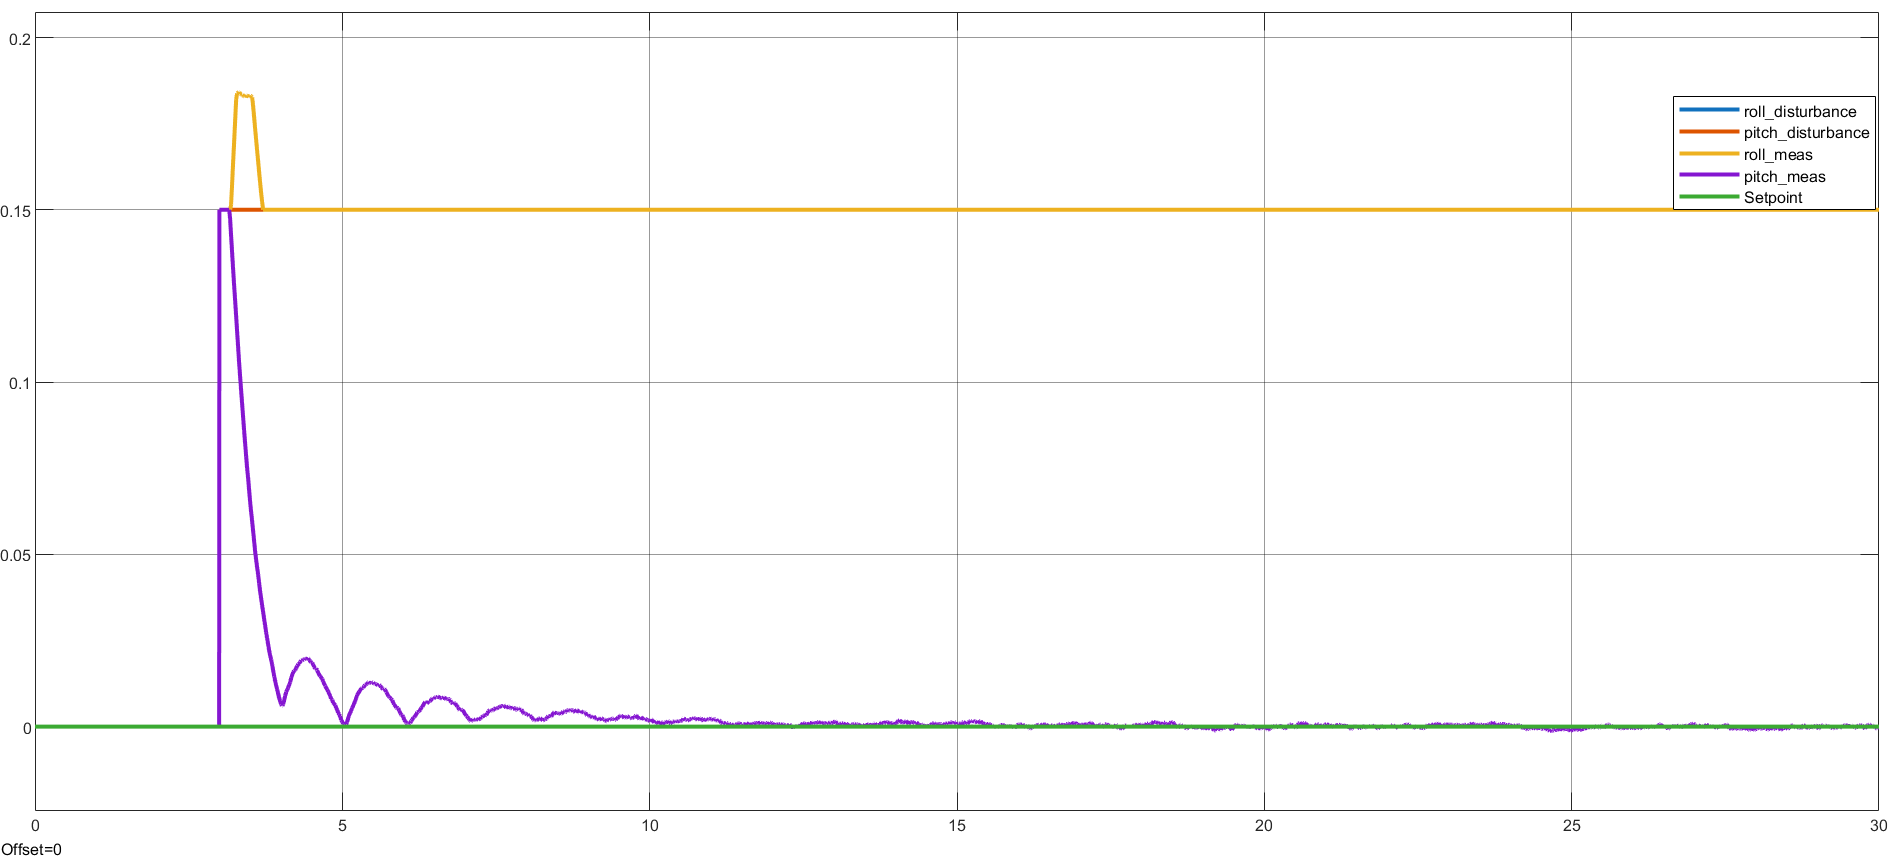
\includegraphics[width=\textwidth]{Images/PID_turning/PID_turning/pitch turning Kp=5 Kd=1.3 Ki=1.6.png}
        \caption{Dùng PID hoàn chỉnh ($K_p=5, K_i=1{,}6, K_d=1{,}3$)}
        \label{fig:pitch_tuning_pid}
    \end{subfigure}
    \caption{Quá trình hiệu chỉnh các khâu P, D, I cho trục Pitch}
    \label{fig:pitch_tuning_process}
\end{figure}

\subsubsection*{Trường hợp sử dụng bộ điều khiển PID hoàn chỉnh (sau khi Tuning)}
Để đánh giá độ ổn định tổng thể sau khi đã hiệu chỉnh, hệ thống được thử nghiệm với tín hiệu nhiễu đồng thời trên cả hai trục. Bộ thông số độc lập là Roll ($K_p=4, K_i=1{,}2, K_d=1{,}3$) và Pitch ($K_p=5, K_i=1{,}6, K_d=1{,}3$). Hình~\ref{fig:pid_noise_step} và Hình~\ref{fig:pid_noise_sine} minh họa đáp ứng của hệ thống dưới tác động của nhiễu bước (step) và nhiễu hình sin.

\begin{figure}[H]
    \centering
    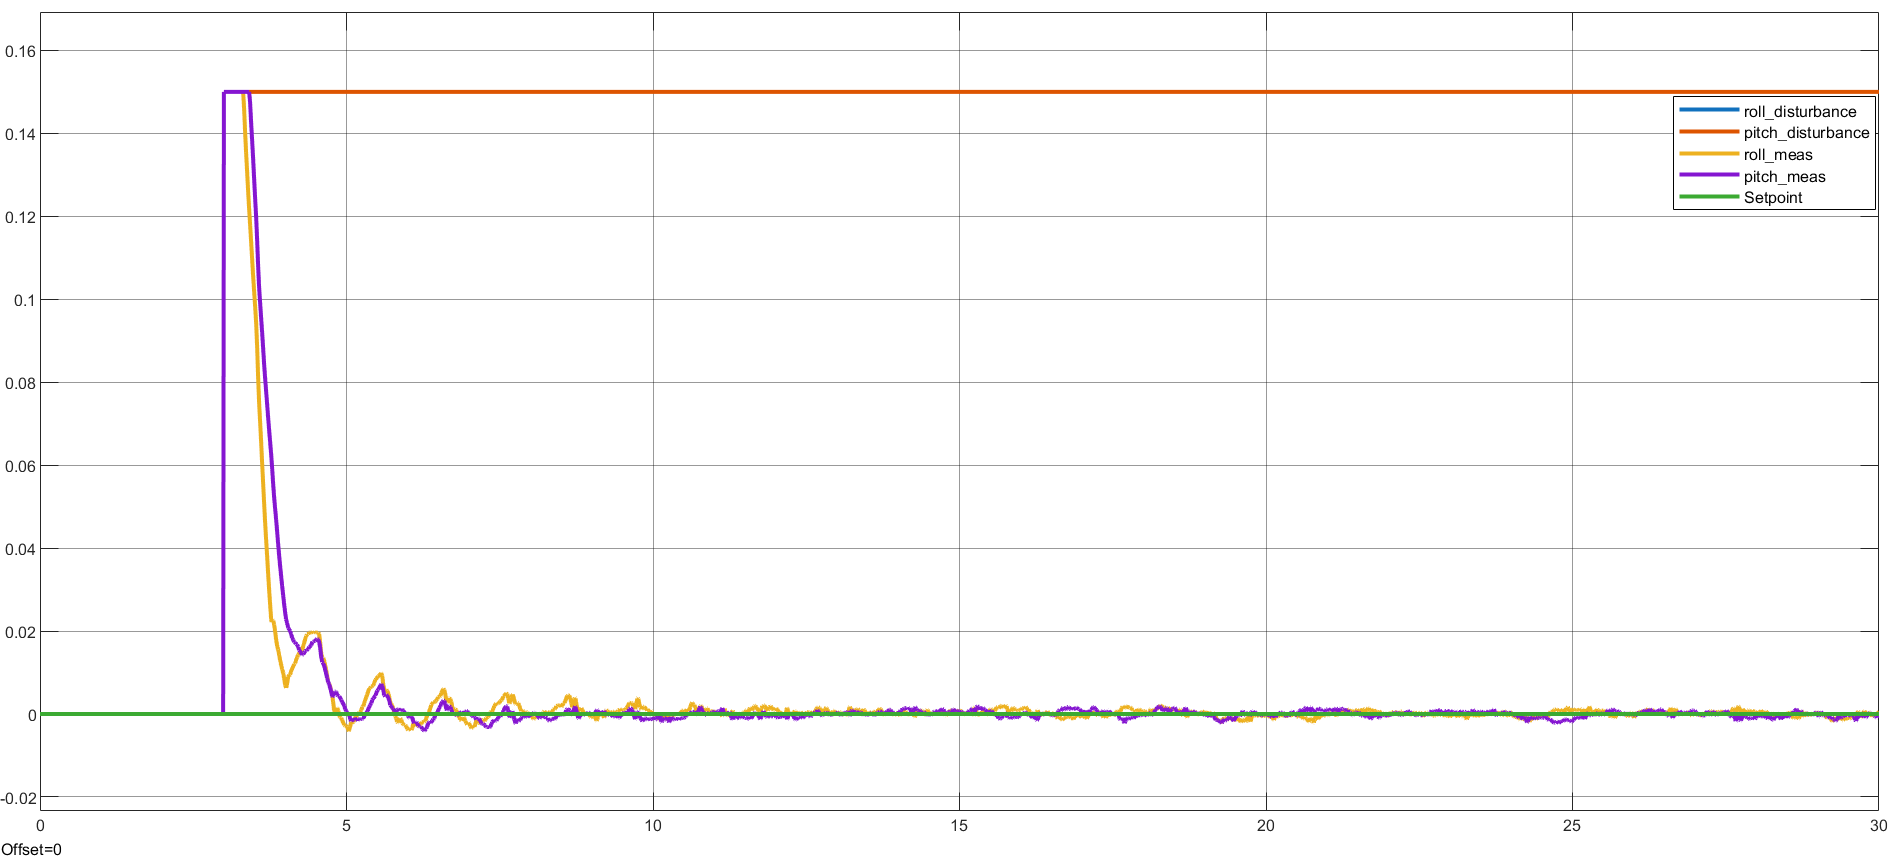
\includegraphics[width=0.8\textwidth]{Images/PID_turning/PID_turning/PID turning nhiễu step.png}
    \caption{Đồ thị đáp ứng hệ thống với tín hiệu nhiễu bước (step) trên cả 2 trục}
    \label{fig:pid_noise_step}
\end{figure}

Từ đồ thị Hình~\ref{fig:pid_noise_step}, tại thời điểm $t = 3$ s, một nhiễu bước có biên độ $0{,}15$ rad được đưa vào hệ thống. Phân tích đồ thị cho thấy ba đặc điểm nổi bật. Thứ nhất, về độ vọt lố (Overshoot), cả hai trục Roll và Pitch đều có độ vọt lố rất nhỏ; khi bù nhiễu, góc vượt qua mốc $0$, đạt giá trị âm lớn nhất khoảng $-0{,}005$ rad. Mức vọt lố này nằm trong giới hạn vô cùng an toàn, đảm bảo robot không bị mất trọng tâm dẫn đến lật ngã. Thứ hai, về thời gian quá độ (Settling Time), hệ thống mất khoảng $7-9$ s (từ $t = 3$ s đến $t = 12$ s) để dập tắt hoàn toàn các dao động và dao động tắt dần quanh giá trị cân bằng, chứng tỏ khả năng đáp ứng khá nhanh trước các thay đổi bất ngờ. Cuối cùng, về sai số xác lập (Steady-state Error), từ sau mốc $t = 12$ s, hệ thống hoàn toàn duy trì được trạng thái thăng bằng với sai số tĩnh xấp xỉ bằng $0$. Điều này minh chứng thành phần khâu tích phân (I) trong bộ điều khiển PID đã hoạt động cực kỳ hiệu quả để triệt tiêu các sai lệch dư.

\begin{figure}[H]
    \centering
    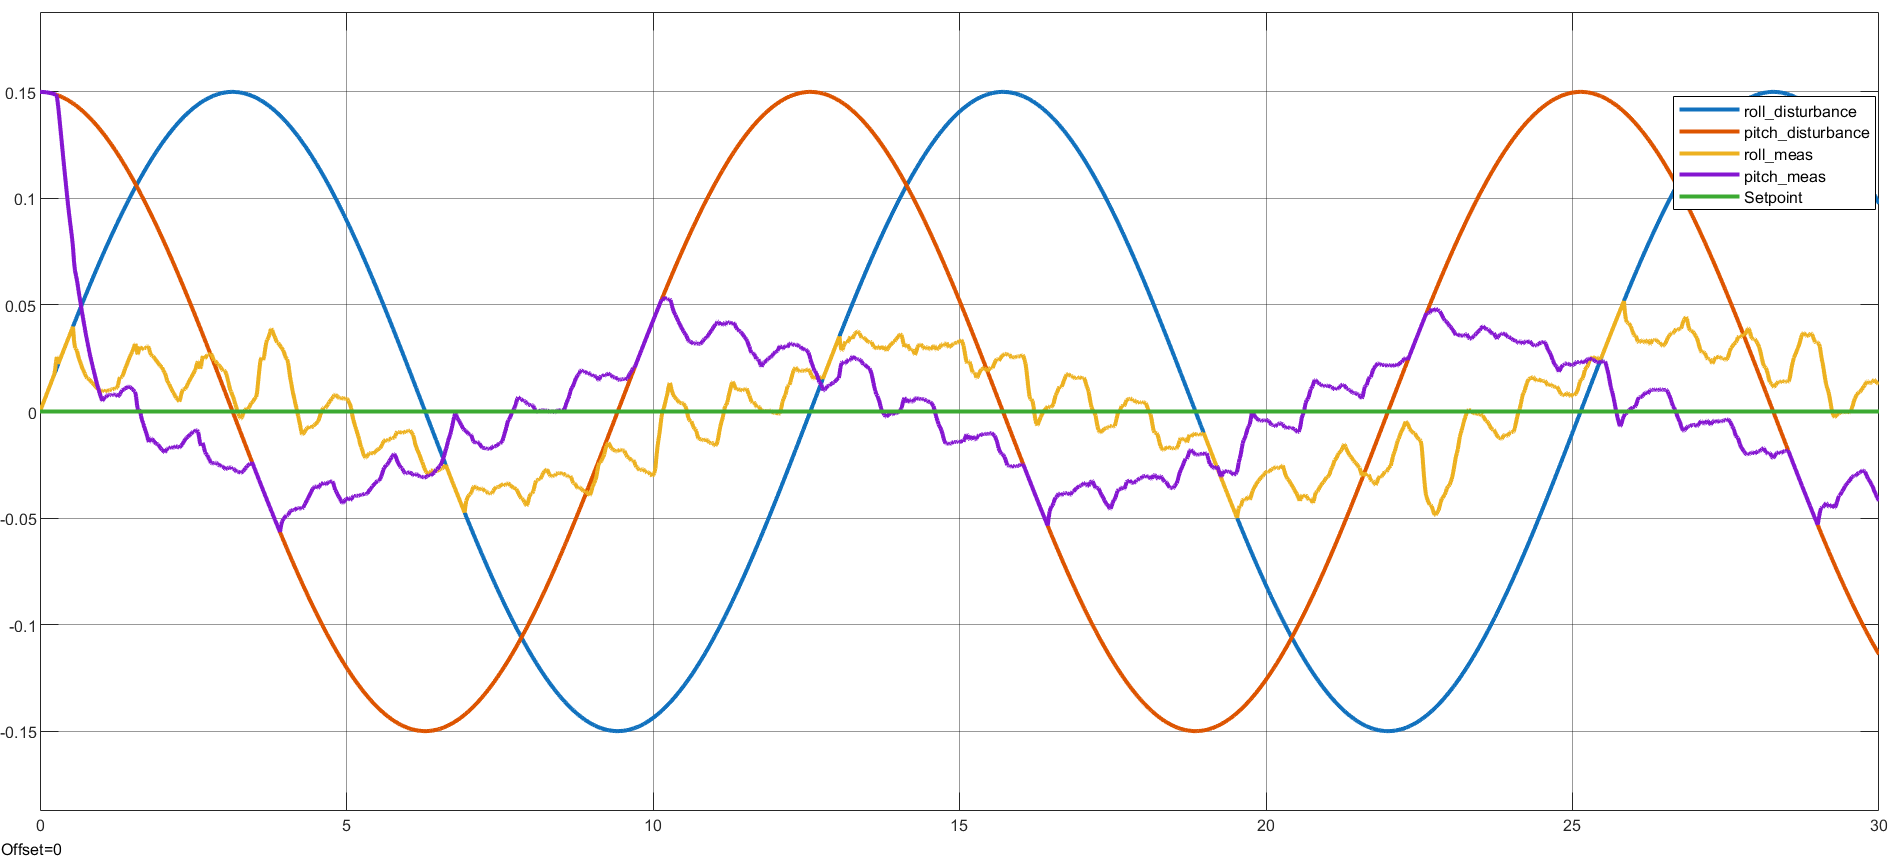
\includegraphics[width=0.8\textwidth]{Images/PID_turning/PID_turning/PID turning nhiễu sin.png}
    \caption{Đồ thị đáp ứng hệ thống với tín hiệu nhiễu hình sin trên cả 2 trục}
    \label{fig:pid_noise_sine}
\end{figure}
\textbf{\textit{Nhận xét so sánh}} 

Trong khi bộ PID có xu hướng đưa quỹ đạo nhanh chóng trở lại ổn định sau một pha "thu chân" và "duỗi chân" mạnh (tương ứng với thời điểm khâu D phản ứng mạnh với độ dốc của nhiễu), thì ở trường hợp bù trực tiếp, hiện tượng này kéo dài và có biên độ thu-duỗi thấp hơn. Sự khác biệt này phản ánh trực tiếp khả năng loại bỏ nhiễu nhanh chóng của một bộ điều khiển có khâu dự báo (D) và khâu tích lũy sai số (I) so với một hệ thống chỉ phản ứng dựa trên sai số tĩnh tại (P).


\subsubsection*{Trường hợp bù sai số trực tiếp ($K_p=1$, $K_i=0$, $K_d=0$)}
Nhằm mục đích đối chiếu hiệu quả của các khâu I và D trong bộ điều khiển PID, một mô phỏng tương tự được thực hiện với trường hợp bù sai số trực tiếp, tương đương thông số $K_p=1, K_i=0, K_d=0$.

\begin{figure}[H]
    \centering
    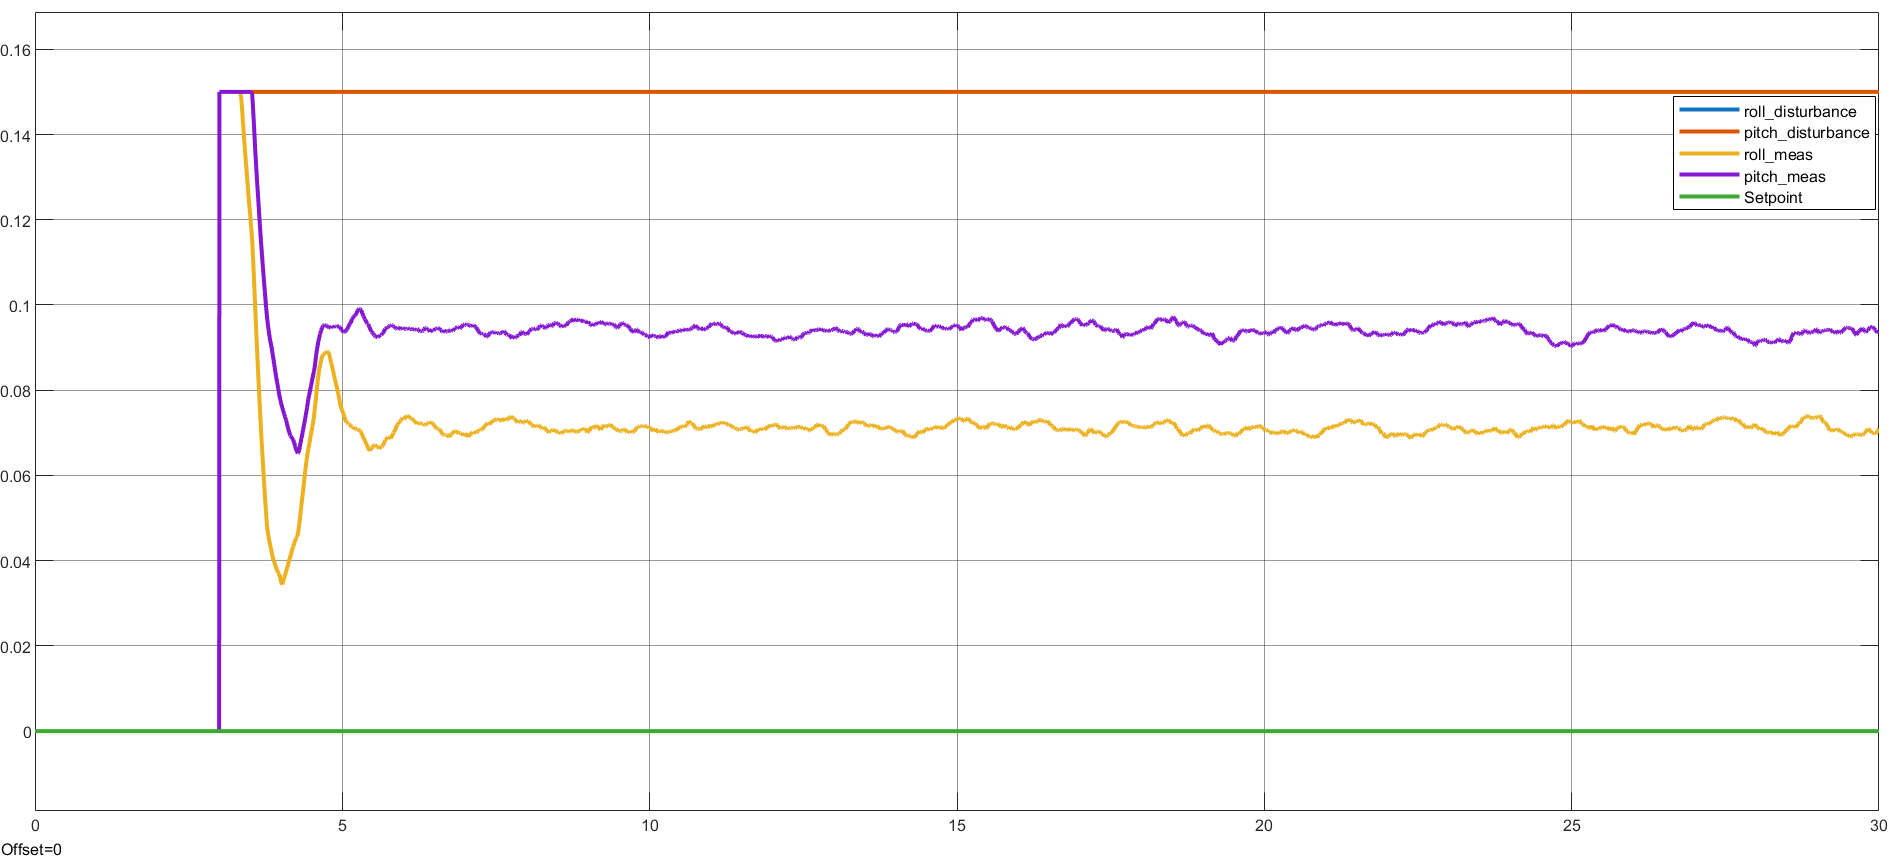
\includegraphics[width=0.8\textwidth]{Images/PID_turning/PID_turning/PID bù trực tiếp Kp=1 step.png}
    \caption{Đồ thị đáp ứng hệ thống với tín hiệu nhiễu bước (step) ($K_p=1, K_i=0, K_d=0$)}
    \label{fig:p_noise_step}
\end{figure}

Từ đồ thị Hình~\ref{fig:p_noise_step}, đồ thị biểu diễn góc nghiêng thực tế đo được (measured angle) của thân robot, khi nhiễu bước có biên độ $D = 0{,}15$ rad tác động vào hệ thống tại $t = 3$ s, thân robot bị nghiêng đi một góc tương ứng. Khảo sát đáp ứng của hệ thống trong trường hợp bù trực tiếp ($K_p=1, K_i=0, K_d=0$) cho thấy sự khác biệt rõ rệt so với bộ điều khiển PID hoàn chỉnh. Trước hết, khác với PID hoàn chỉnh, trường hợp bù trực tiếp hoàn toàn không có độ vọt lố qua mốc cân bằng $0$; góc nghiêng đo được giảm dần nhưng chưa bao giờ đạt tới hay vượt qua mốc $0$ rad. Bên cạnh đó, về dao động và thời gian quá độ, mặc dù không vượt qua mốc $0$, hệ thống lại xuất hiện trạng thái dao động (oscillatory behavior) kéo dài. Hiện tượng này xảy ra do sự vắng mặt của thành phần vi phân (D), vốn đóng vai trò dự báo và triệt tiêu sự thay đổi đột ngột của sai lệch. Hậu quả là, nếu không có khâu D, hệ thống mất hơn $15$ s để các dao động suy giảm và ổn định trở lại. Nghiêm trọng nhất là vấn đề sai số xác lập; sau thời gian quá độ, góc nghiêng xác lập ở mức khá cao, dao động quanh $0{,}07$ rad đối với Roll và $0{,}05$ rad đối với Pitch. Hệ thống vòng kín tỷ lệ 1:1 không thể bù trừ triệt để lượng nhiễu đầu vào, từ đó đòi hỏi bắt buộc phải tích hợp khâu tích phân (I) nhằm duy trì tín hiệu bù kể cả khi góc nghiêng tiến về $0$.

\begin{figure}[H]
    \centering
    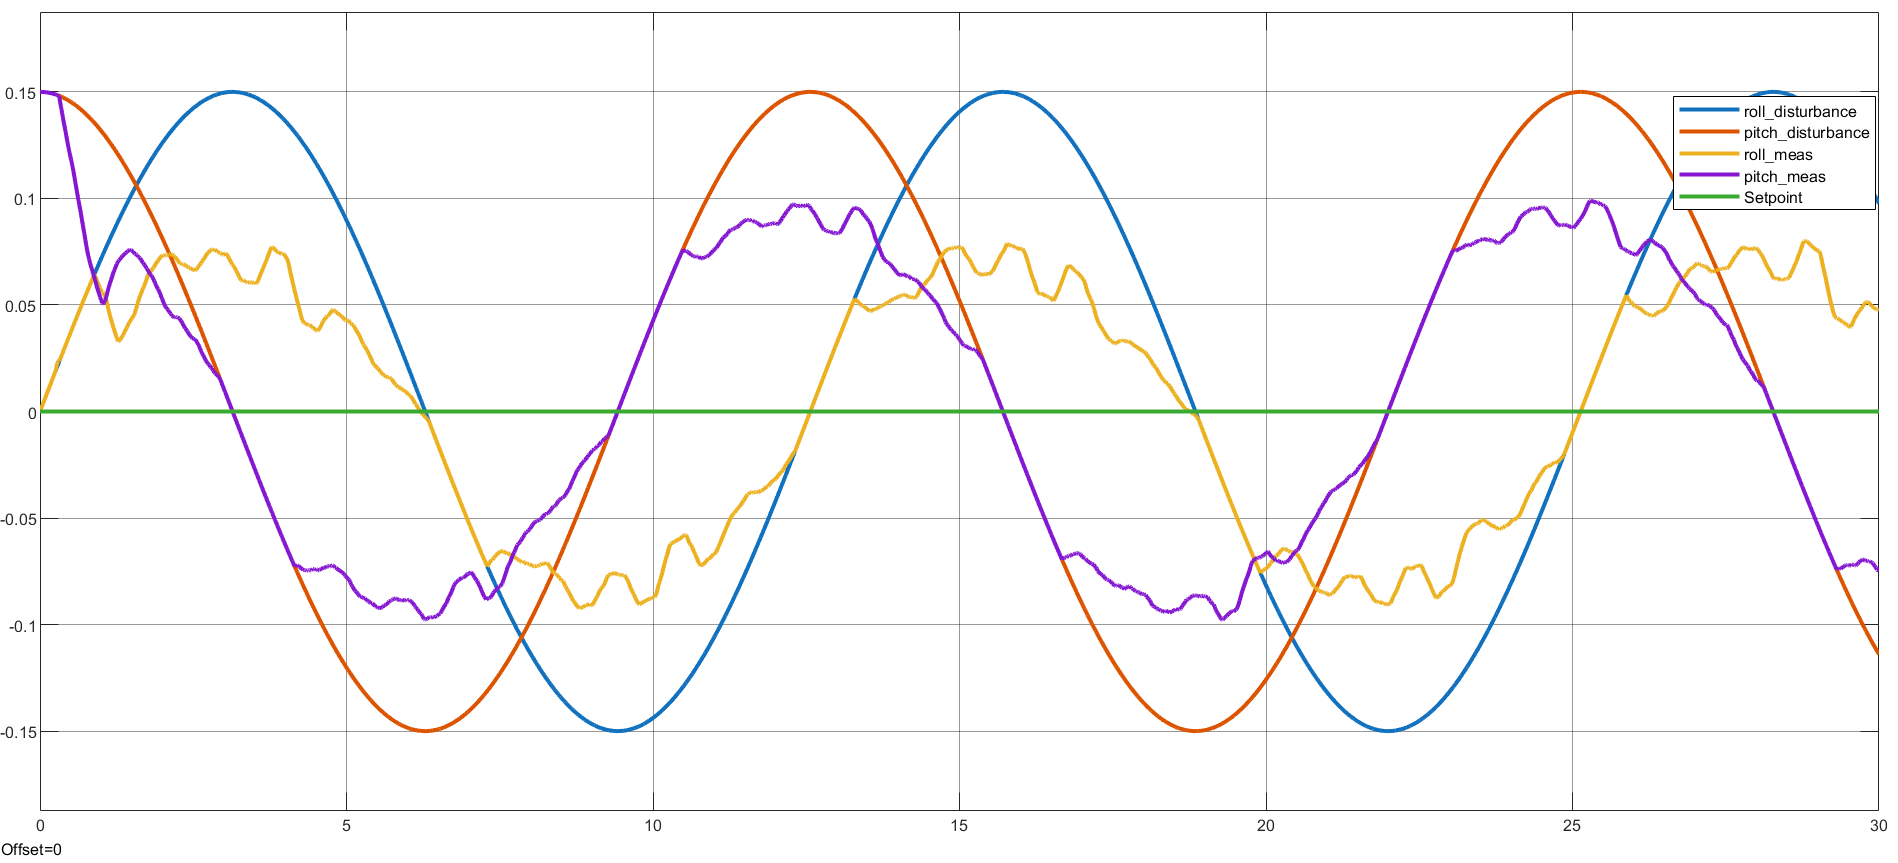
\includegraphics[width=0.8\textwidth]{Images/PID_turning/PID_turning/PID bù trực tiếp Kp=1 sin.png}
    \caption{Đồ thị đáp ứng hệ thống với tín hiệu nhiễu hình sin ($K_p=1, K_i=0, K_d=0$)}
    \label{fig:p_noise_sine}
\end{figure}

\textbf{\textit{Nhận xét so sánh}}

Thông qua việc đối chiếu giữa bộ điều khiển PID độc lập hai trục và cấu hình bù trực tiếp vòng kín ($K_p=1, K_i=0, K_d=0$), có thể khẳng định tính tất yếu của việc tuning riêng biệt các khâu I và D. Tư duy bù trực tiếp để lại sai số xác lập quá lớn và gây ra dao động kéo dài do vắng mặt khâu vi phân. Ngược lại, bộ PID hoàn chỉnh đã loại bỏ triệt để sai số xác lập, khống chế vọt lố ở mức cực nhỏ (âm $\sim 0{,}005$ rad) và xác lập tính ổn định nhanh chóng.

Các Hình~\ref{fig:pid_response_7}, Hình~\ref{fig:pid_response_8} và Hình~\ref{fig:pid_response_9} trình bày các tín hiệu nội bộ thu được trong quá trình mô phỏng khi robot thực hiện chu trình di chuyển có tính tuần hoàn (dáng đi Trot).

Hình~\ref{fig:pid_response_7} thể hiện quỹ đạo tọa độ trục Z (\texttt{z\_out}) của 4 bàn chân robot theo thời gian, cho thấy sự kết hợp giữa quỹ đạo bước đi cơ sở và tín hiệu bù từ bộ điều khiển PID. Cụ thể, trước thời điểm $t = 3$ s, cả 4 chân đều có chung một biên dạng ổn định, trong đó pha chống chân nằm ở mức âm cơ sở, và pha vung chân tạo thành các đỉnh nhọn nhấc lên đều đặn. Tuy nhiên, từ thời điểm $t = 3$ s, khi nhiễu nghiêng xuất hiện, đồ thị bắt đầu phân hóa rõ rệt với đường cơ sở nhảy vọt và các đỉnh vung chân hướng xuống mạnh mẽ. Hiện tượng này được giải thích bởi nguyên lý động học (Kinematic Coupling): sự cộng hưởng của nhiễu Roll và Pitch khi robot bị nghiêng mạnh khiến một số điểm chân bị ép sát xuống mặt đất nhất. Để bù trừ, PID ra lệnh thu chân lại cực hạn. Trong tư thế gập sâu này, kết hợp với việc hệ trục tọa độ thân robot đã bị nghiêng lớn, động tác vung chân về phía trước bị "khớp nối động học" và chuyển hóa thành chuyển động duỗi dài ra theo trục Z của thân robot để có thể chạm tới điểm đặt chân mong muốn. Chuỗi phản ứng này minh họa rõ rệt giới hạn không gian làm việc (workspace boundary) và tính chất phức tạp của robot bốn chân dưới tác động của sai lệch tư thế lớn.

\begin{figure}[H]
    \centering
    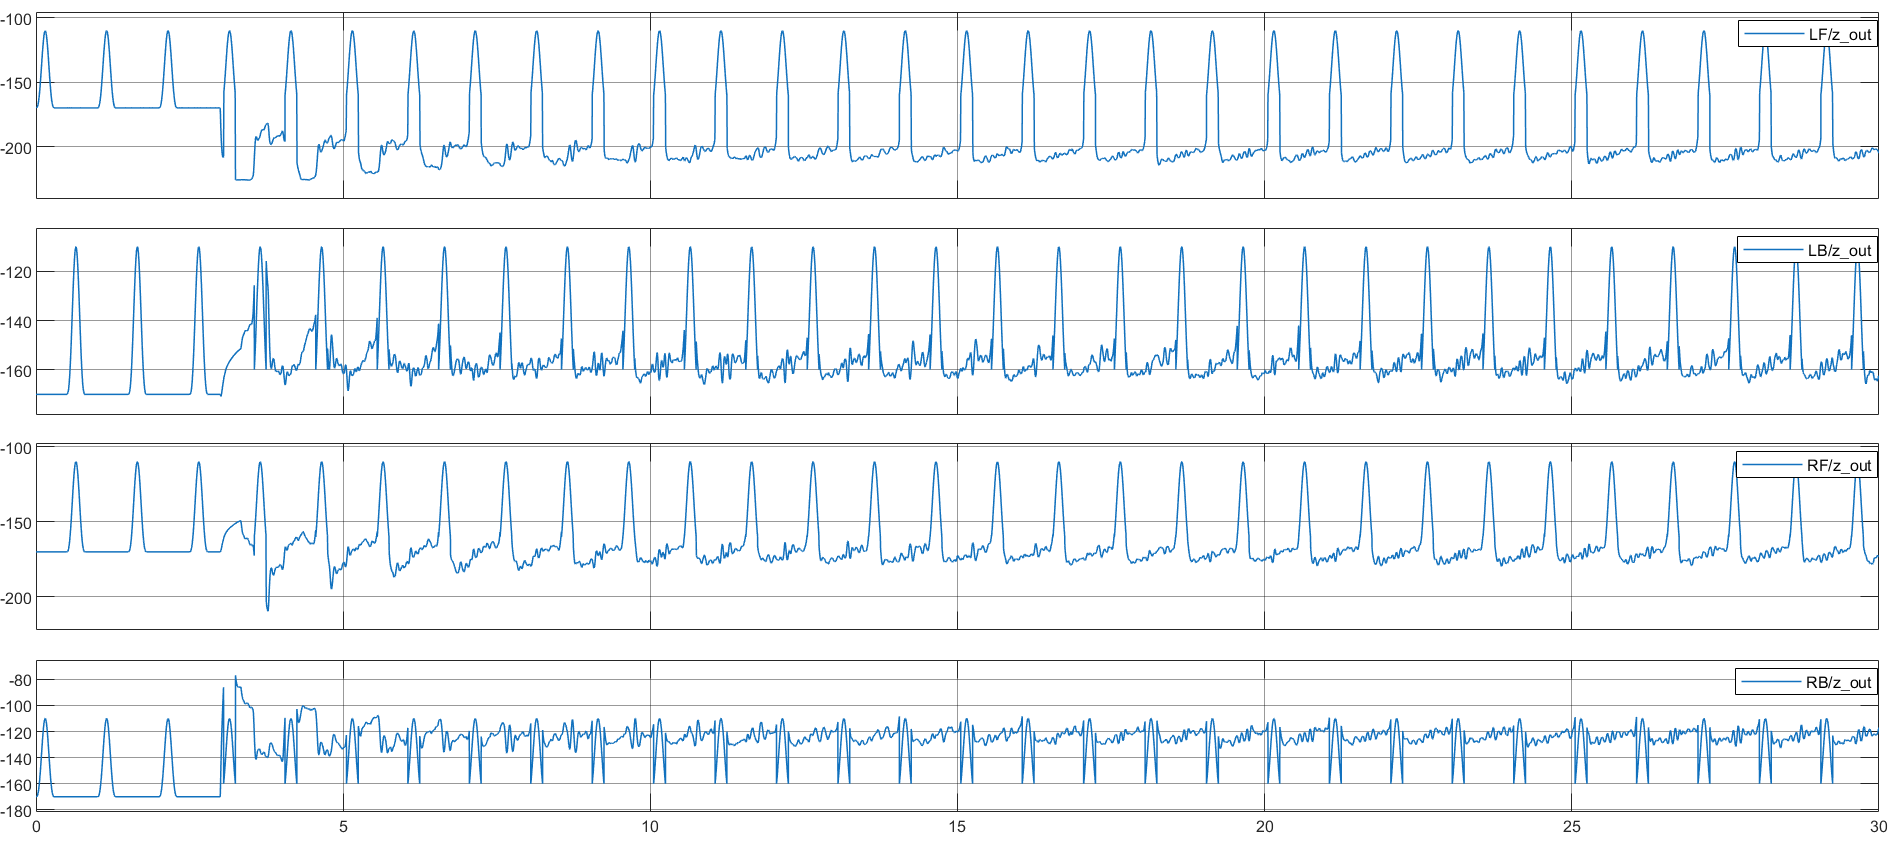
\includegraphics[width=0.8\textwidth]{Images/PID_turning/PID_turning/zout.png}
    \caption{Đồ thị tín hiệu vị trí cao độ bàn chân trục Z (\texttt{z\_out}) của 4 chân robot}
    \label{fig:pid_response_7}
\end{figure}

Các Hình~\ref{fig:pid_response_8} và Hình~\ref{fig:pid_response_9} minh họa quá trình tiền xử lý tín hiệu bên trong bộ điều khiển PID góc Roll và Pitch nhằm phân lập sai lệch tư thế khỏi các dao động sinh ra do chu trình bước đi. Quá trình bắt đầu với tín hiệu \texttt{roll\_meas} và \texttt{pitch\_meas}, vốn bao gồm các dao động tuần hoàn biên độ lớn do sự dịch chuyển trọng tâm luân phiên giữa các chân. Tín hiệu này sau đó đi qua bộ lọc trung bình trượt hàm mũ (EMA) để làm suy giảm các nhiễu rung động cơ học tần số cao do va đập, giúp bảo toàn sóng cơ bản của dáng đi. Tiếp đến, bộ lọc trung bình (Avg) đóng vai trò then chốt như một bộ lọc thông thấp (Low-pass Filter). Ví dụ tại $t = 3$ s, khi nhiễu bước tác động vào hệ thống, bộ lọc Avg đã triệt tiêu phần lớn dao động của dáng đi và trích xuất thành công độ trôi dạt tư thế (baseline drift). Cuối cùng, tín hiệu đi qua khâu vùng chết (Deadzone) để cắt xén phần vi sai dư thừa, minh chứng rằng bộ điều khiển đã trích xuất được mức sai số tư thế hữu ích và chính xác nhằm đưa vào khâu tính toán PID, qua đó loại bỏ hoàn toàn hiện tượng phản ứng quá mức với các dao động tự nhiên.
Dựa trên chuỗi tín hiệu đã được xử lý này, bộ điều khiển PID tính toán phản hồi chuẩn xác mà không phá vỡ động học di chuyển tự nhiên của robot.

\begin{figure}[H]
    \centering
    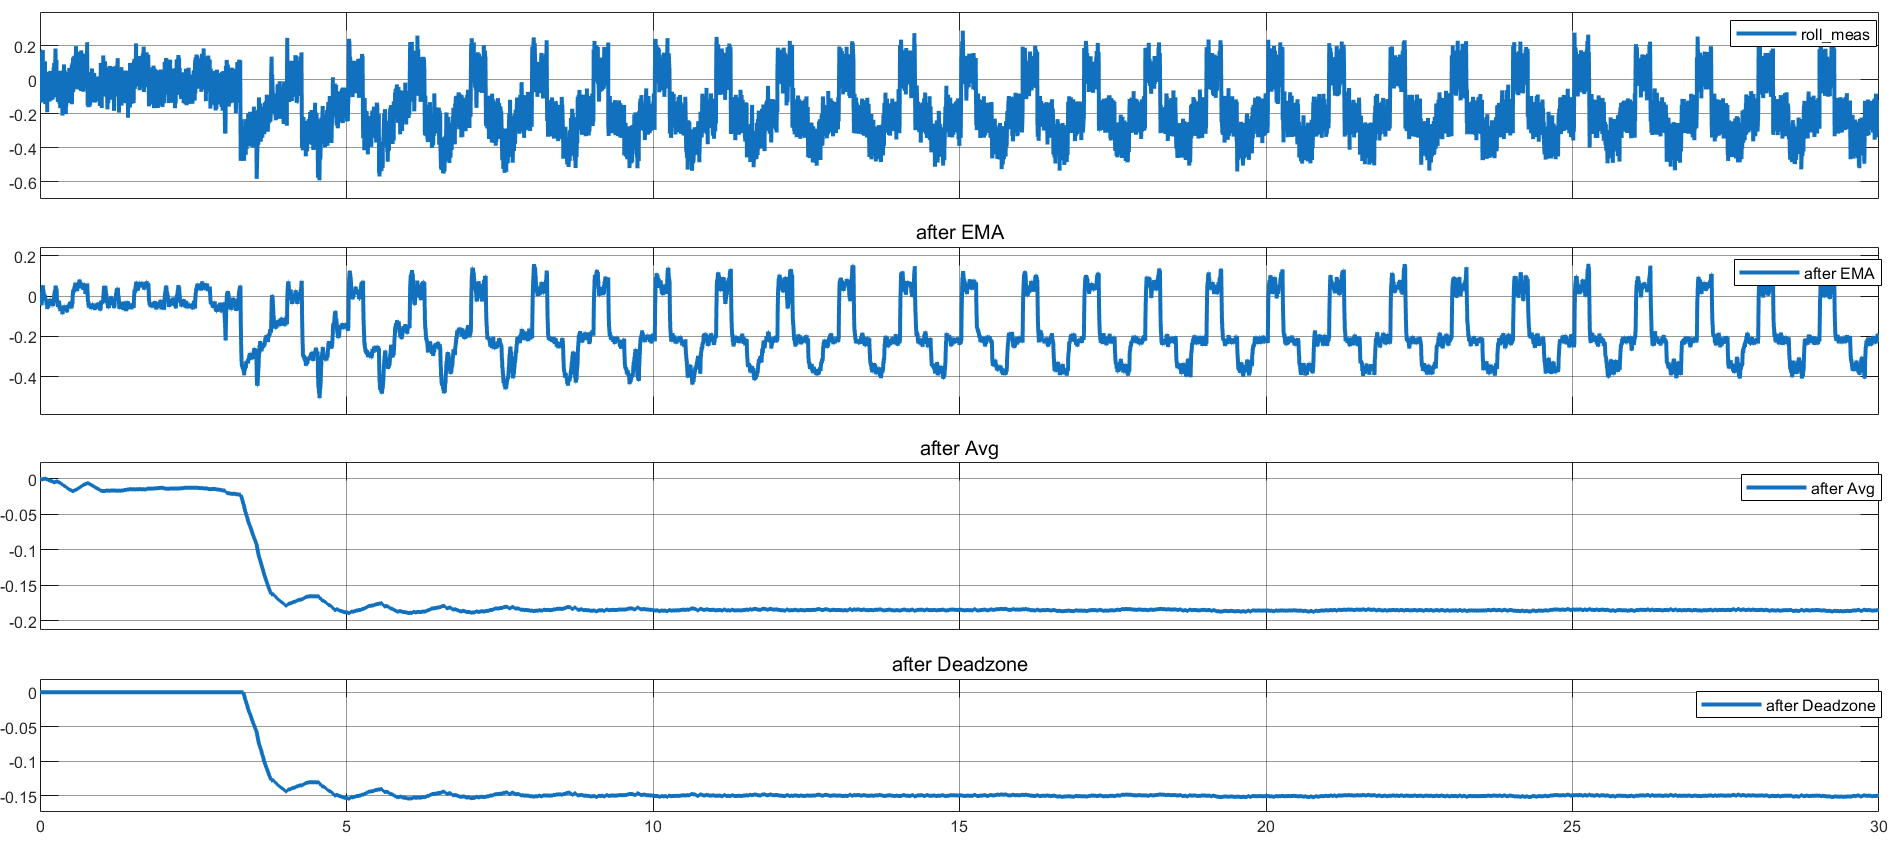
\includegraphics[width=0.8\textwidth]{Images/PID_turning/PID_turning/xử lí roll trước khi đưa vào PID.png}
    \caption{Đồ thị các tín hiệu xử lý nội bộ của bộ điều khiển PID góc Roll}
    \label{fig:pid_response_8}
\end{figure}

\begin{figure}[H]
    \centering
    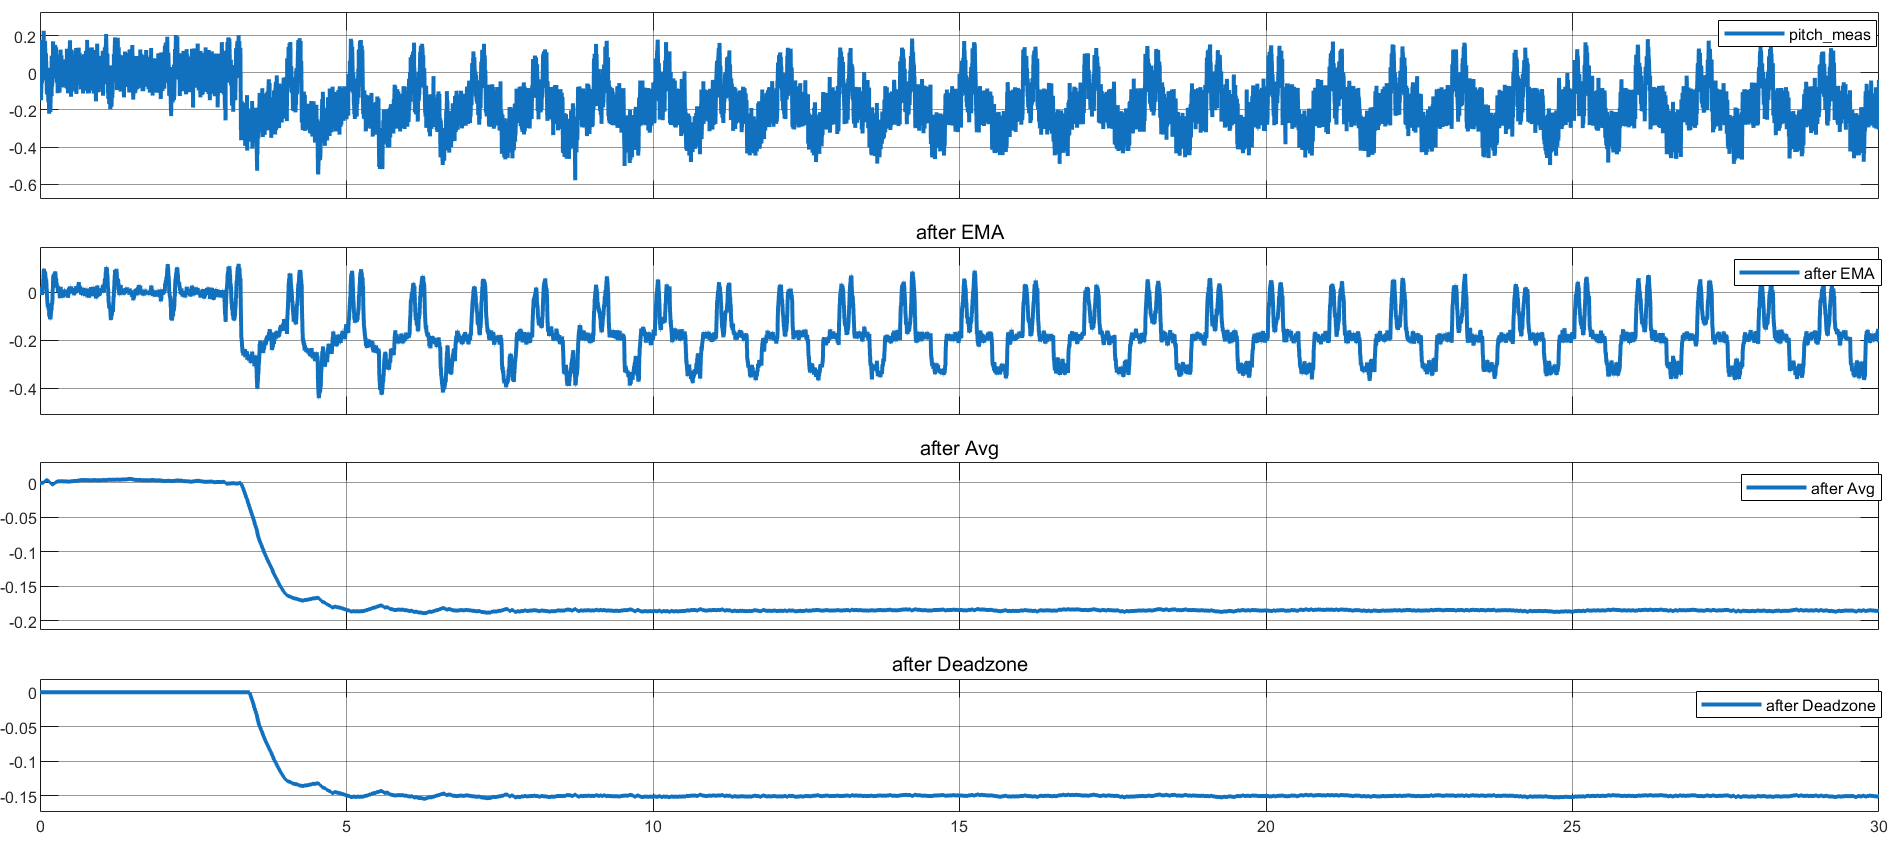
\includegraphics[width=0.8\textwidth]{Images/PID_turning/PID_turning/xử lí pitch trước khi đưa vào PID.png}
    \caption{Đồ thị các tín hiệu xử lý nội bộ của bộ điều khiển PID góc Pitch}
    \label{fig:pid_response_9}
\end{figure}

\section{Cấu hình môi trường mô phỏng Gazebo}

\subsection{Mô hình robot URDF}

Robot bốn chân được mô tả bằng file URDF (Unified Robot Description Format), định nghĩa đầy đủ cấu trúc cơ khí bao gồm 13 link (1 thân + 12 khâu chân) và 12 khớp quay (revolute joint). Mỗi link được gán các thuộc tính quán tính (khối lượng $m$, ma trận quán tính $I$), hình dạng va chạm (collision geometry) và hình dạng hiển thị (visual geometry) sử dụng file mesh STL.

Các tham số hình học chính của mô hình URDF được trình bày trong Bảng~\ref{tab:urdf_params}.

\begin{table}[H]
\centering
\caption{Tham số hình học mô hình URDF}
\label{tab:urdf_params}
\renewcommand{\arraystretch}{1.3}
\begin{tabular}{|l|c|c|l|}
\hline
\textbf{Tham số} & \textbf{Ký hiệu} & \textbf{Giá trị} & \textbf{Đơn vị} \\ \hline
Chiều dài thân & $L$ & 209 & mm \\ \hline
Chiều rộng thân & $W$ & 191 & mm \\ \hline
Chiều dài khớp coxa & $l_1$ & 26 & mm \\ \hline
Chiều dài xương đùi & $l_2$ & 106 & mm \\ \hline
Chiều dài xương ống chân & $l_3$ & 125 & mm \\ \hline
Khối lượng thân & $m_{body}$ & 1,5 & kg \\ \hline
Khối lượng mỗi link chân & $m_{leg}$ & 0,05--0,15 & kg \\ \hline
Giới hạn effort khớp hip & $\tau_{max,hip}$ & 2,94 & Nm \\ \hline
Giới hạn effort khớp tibia & $\tau_{max,tibia}$ & 1,96 & Nm \\ \hline
\end{tabular}
\end{table}

Kích thước URDF trong mô phỏng được cập nhật để khớp hoàn toàn với robot thực tế ($L=209$ mm, $W=191$ mm, $l_1=26$ mm, $l_2=106$ mm, $l_3=125$ mm). Điều này đảm bảo tính nhất quán cao nhất giữa mô phỏng và phần cứng.

\subsection{Plugin điều khiển Gazebo}

Giao diện điều khiển giữa ROS~2 và Gazebo sử dụng plugin \texttt{gazebo\_ros2\_control} với cấu hình effort command interface. Trong chế độ này, ROS~2 gửi giá trị mô-men xoắn (effort, đơn vị Nm) trực tiếp đến các khớp trong Gazebo, thay vì gửi vị trí hoặc vận tốc. Bộ điều khiển PD cấp thấp được triển khai phía ROS~2 để chuyển đổi sai lệch vị trí thành mô-men:

\begin{equation}
    \tau_i = K_p (\theta_{target,i} - \theta_{actual,i}) - K_d \cdot \omega_{actual,i}
\end{equation}

trong đó $\theta_{target,i}$ là góc mong muốn từ IK, $\theta_{actual,i}$ và $\omega_{actual,i}$ là vị trí và vận tốc góc thực tế đọc từ Gazebo.

\subsection{Cấu hình vật lý và môi trường}

Môi trường mô phỏng được cấu hình chặt chẽ với các tham số vật lý chuyên dụng. Hệ thống sử dụng engine vật lý ODE (Open Dynamics Engine) chạy ở bước thời gian $\Delta t = 1$ ms, tương đương tần số 1000 Hz. Trọng lực được thiết lập ở mức chuẩn $g = 9{,}81$ m/s$^2$ tác dụng theo phương $-z$, kết hợp với mặt phẳng đất vô hạn tại $z = 0$ (không có địa hình nhấp nhô) và có hệ số ma sát Coulomb $\mu = 0{,}8$ nhằm mô phỏng bề mặt nhám. Ngoài ra, cảm biến IMU ảo được tích hợp thông qua plugin \texttt{libgazebo\_ros\_imu\_sensor.so}, chịu trách nhiệm cung cấp dữ liệu quaternion, vận tốc góc và gia tốc tuyến tính tại tần số 100 Hz. Cảm biến này cũng được thêm nhiễu Gaussian, cụ thể $\sigma = 0{,}001$ rad/s đối với con quay hồi chuyển và $\sigma = 0{,}01$ m/s$^2$ đối với gia tốc kế, nhằm phản ánh chính xác các giới hạn của cảm biến vật lý.

Tốc độ cập nhật bộ điều khiển ROS~2 được đặt ở 1000 Hz ($f_{ctrl} = 1000$ Hz), đồng bộ với bước thời gian vật lý của Gazebo. Chu kỳ timer của Gait Generator node là 3 ms, tương ứng với tần số xuất lệnh quỹ đạo 333 Hz.

\subsection{Kết quả mô phỏng vận động cơ bản}

Sau khi cấu hình xong môi trường, các thử nghiệm vận động cơ bản được tiến hành trên Gazebo để đánh giá khả năng di chuyển động học trước khi phân tích sâu vào hệ thống điều khiển.

Hình \ref{fig:sim_home} minh họa chuỗi hình ảnh quá trình khởi tạo tư thế đứng chuẩn của robot từ lúc khởi động trên hệ thống mô phỏng Gazebo.

\begin{figure}[H]
    \centering
    \begin{subfigure}[b]{0.19\textwidth}
        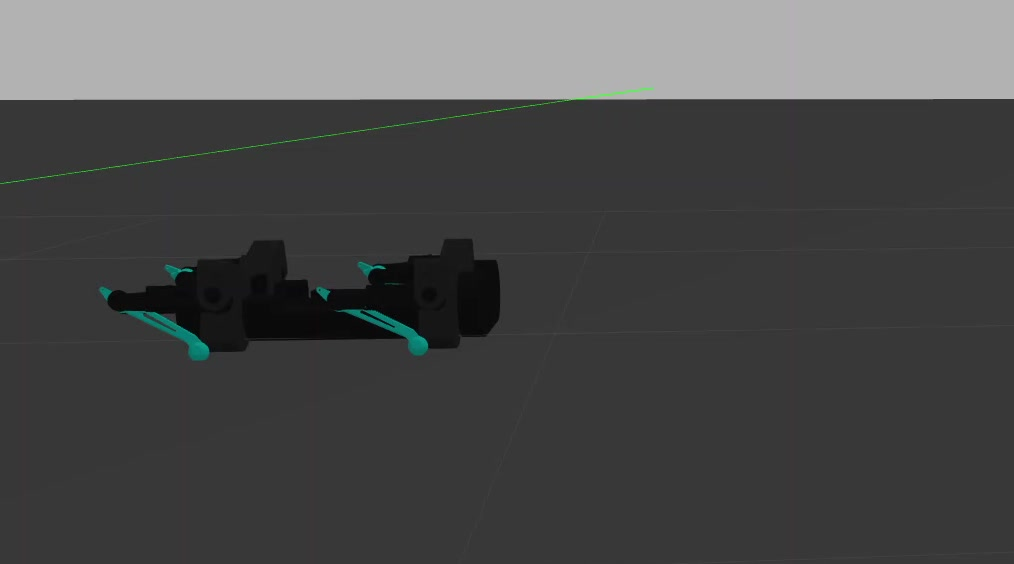
\includegraphics[width=\textwidth]{real_robot/gait/frames_cropped/1.jpg}
        \caption{$t=0.1$ s}
    \end{subfigure}
    \hfill
    \begin{subfigure}[b]{0.19\textwidth}
        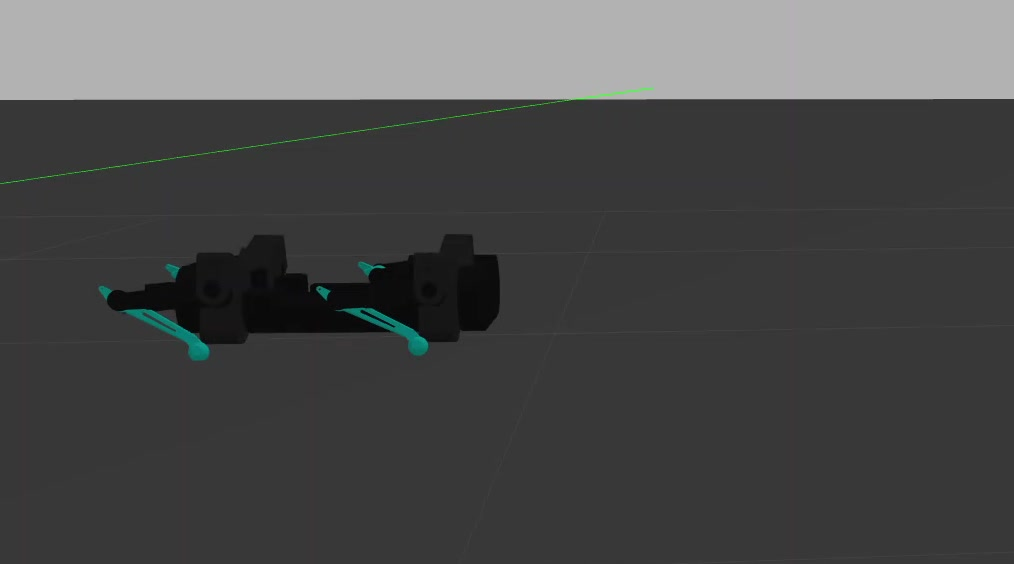
\includegraphics[width=\textwidth]{real_robot/gait/frames_cropped/2.jpg}
        \caption{$t=0.2$ s}
    \end{subfigure}
    \hfill
    \begin{subfigure}[b]{0.19\textwidth}
        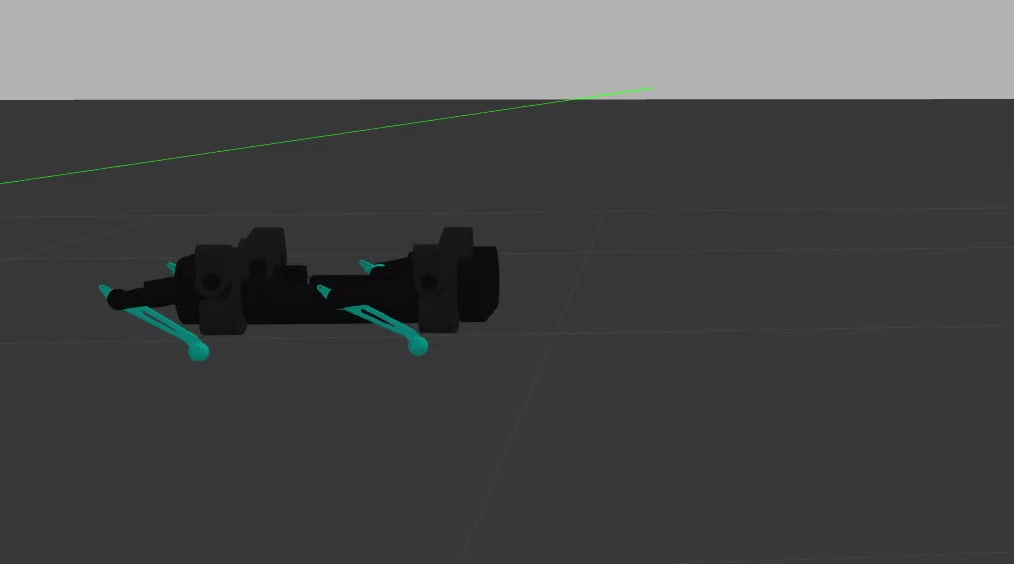
\includegraphics[width=\textwidth]{real_robot/gait/frames_cropped/3.jpg}
        \caption{$t=0.3$ s}
    \end{subfigure}
    \hfill
    \begin{subfigure}[b]{0.19\textwidth}
        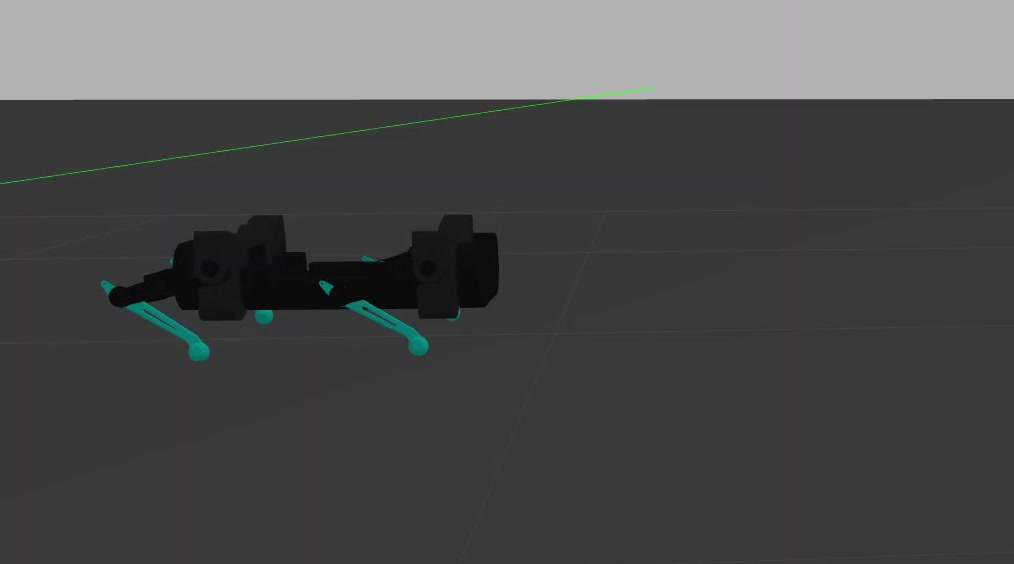
\includegraphics[width=\textwidth]{real_robot/gait/frames_cropped/4.jpg}
        \caption{$t=0.4$ s}
    \end{subfigure}
    \hfill
    \begin{subfigure}[b]{0.19\textwidth}
        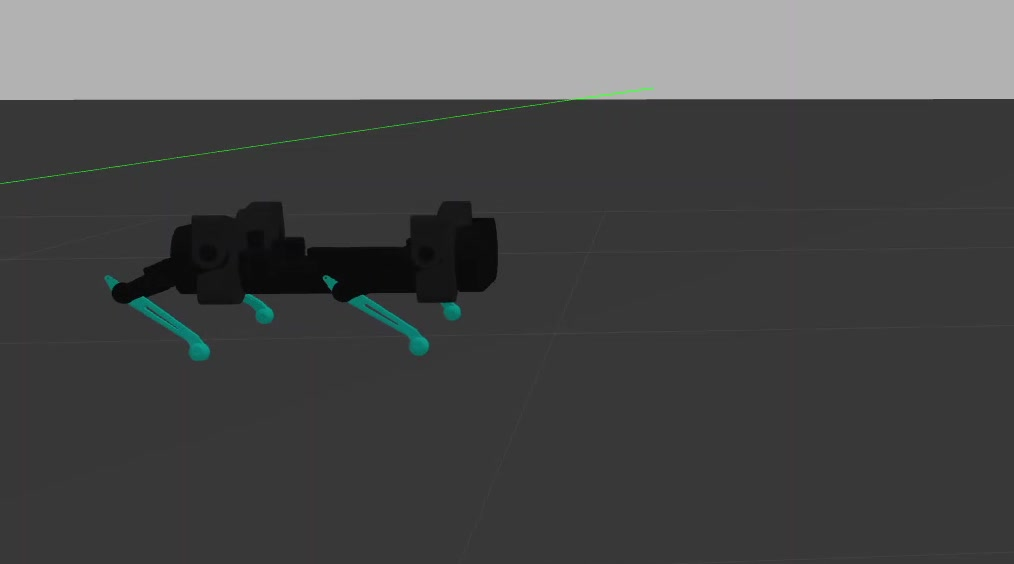
\includegraphics[width=\textwidth]{real_robot/gait/frames_cropped/5.jpg}
        \caption{$t=0.5$ s}
    \end{subfigure}
    
    \vspace{0.2cm}
    \begin{subfigure}[b]{0.19\textwidth}
        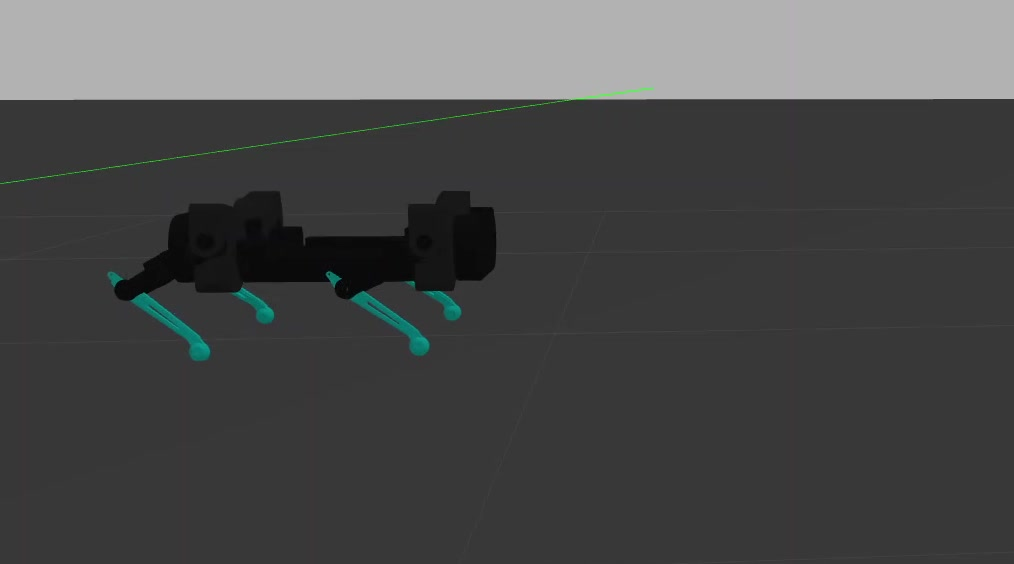
\includegraphics[width=\textwidth]{real_robot/gait/frames_cropped/6.jpg}
        \caption{$t=0.6$ s}
    \end{subfigure}
    \hfill
    \begin{subfigure}[b]{0.19\textwidth}
        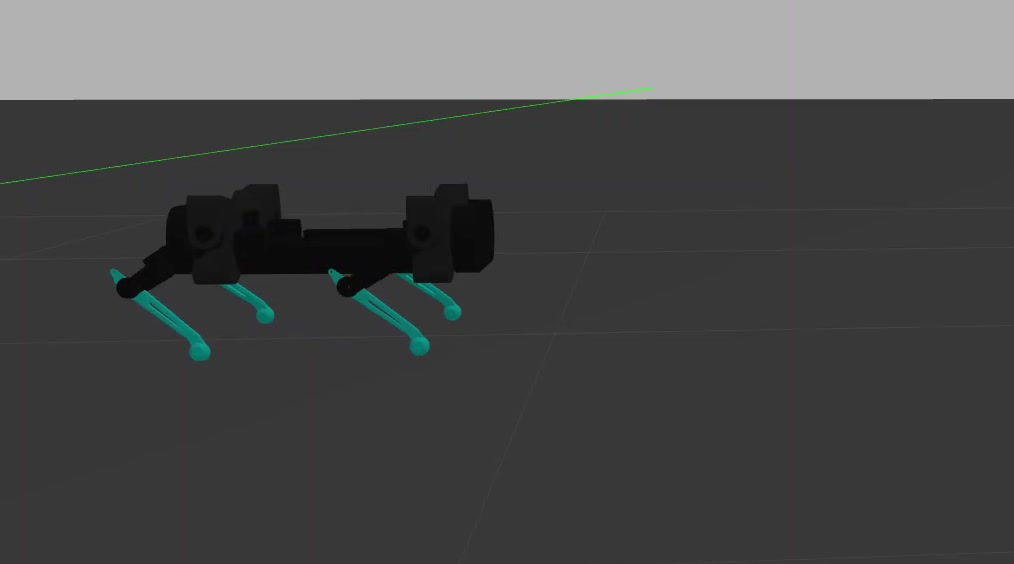
\includegraphics[width=\textwidth]{real_robot/gait/frames_cropped/7.jpg}
        \caption{$t=0.7$ s}
    \end{subfigure}
    \hfill
    \begin{subfigure}[b]{0.19\textwidth}
        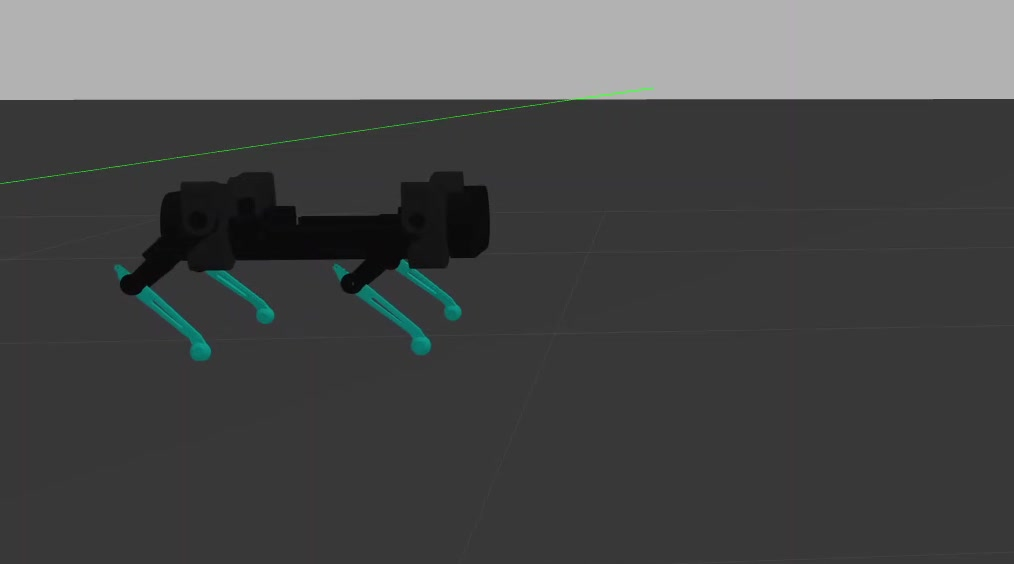
\includegraphics[width=\textwidth]{real_robot/gait/frames_cropped/8.jpg}
        \caption{$t=0.8$ s}
    \end{subfigure}
    \hfill
    \begin{subfigure}[b]{0.19\textwidth}
        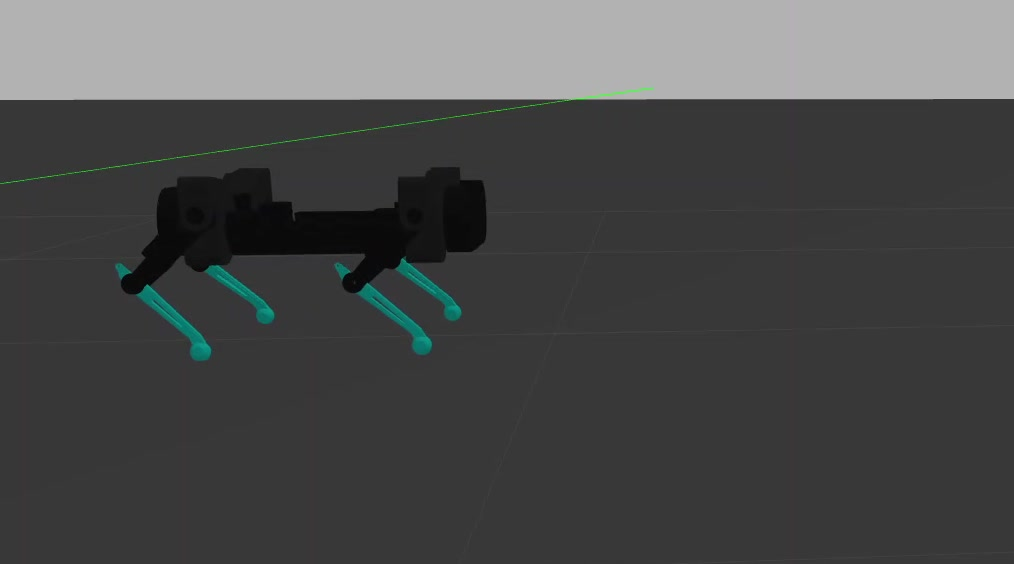
\includegraphics[width=\textwidth]{real_robot/gait/frames_cropped/9.jpg}
        \caption{$t=0.9$ s}
    \end{subfigure}
    \hfill
    \begin{subfigure}[b]{0.19\textwidth}
        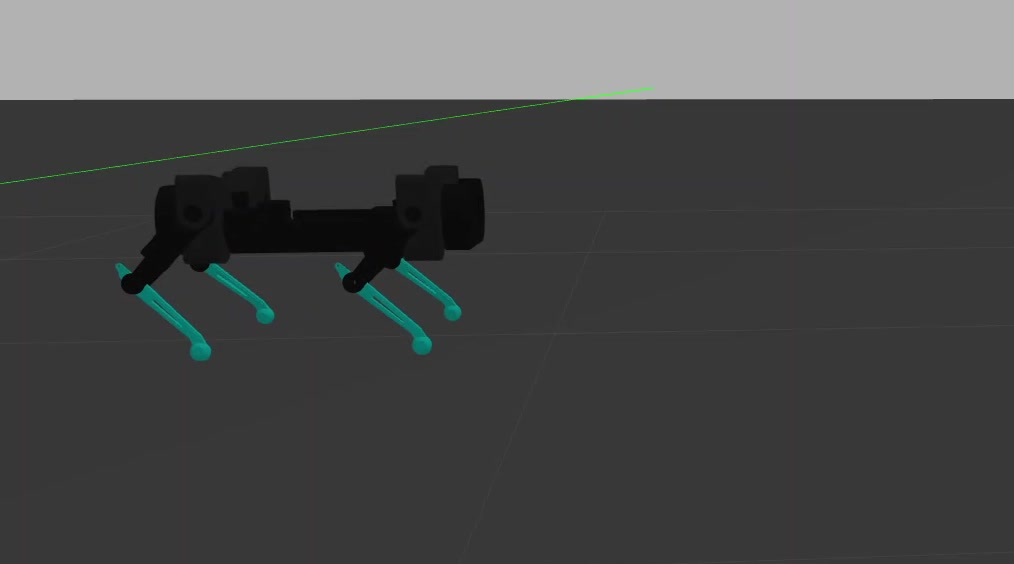
\includegraphics[width=\textwidth]{real_robot/gait/frames_cropped/10.jpg}
        \caption{$t=1.0$ s}
    \end{subfigure}
    \caption{Chuỗi chuyển động quá trình khởi tạo tư thế đứng của robot trên mô phỏng Gazebo.}
    \label{fig:sim_home}
\end{figure}


Hình \ref{fig:sim_trot_sequence} ghi lại chuỗi hình ảnh của robot khi thực hiện dáng đi Trot trên hệ thống mô phỏng Gazebo. Các pha luân phiên nhấc chân và chống chân được thể hiện rõ ràng.

\begin{figure}[H]
    \centering
    \begin{subfigure}[b]{0.19\textwidth}
        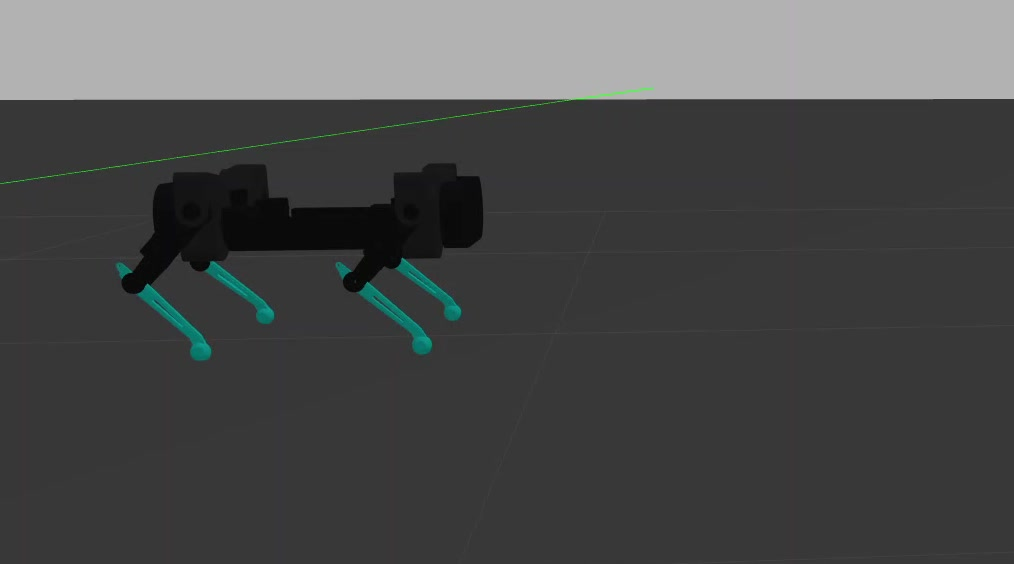
\includegraphics[width=\textwidth]{real_robot/gait/frames_cropped/20.jpg}
        \caption{$t=2.0$ s}
    \end{subfigure}
    \hfill
    \begin{subfigure}[b]{0.19\textwidth}
        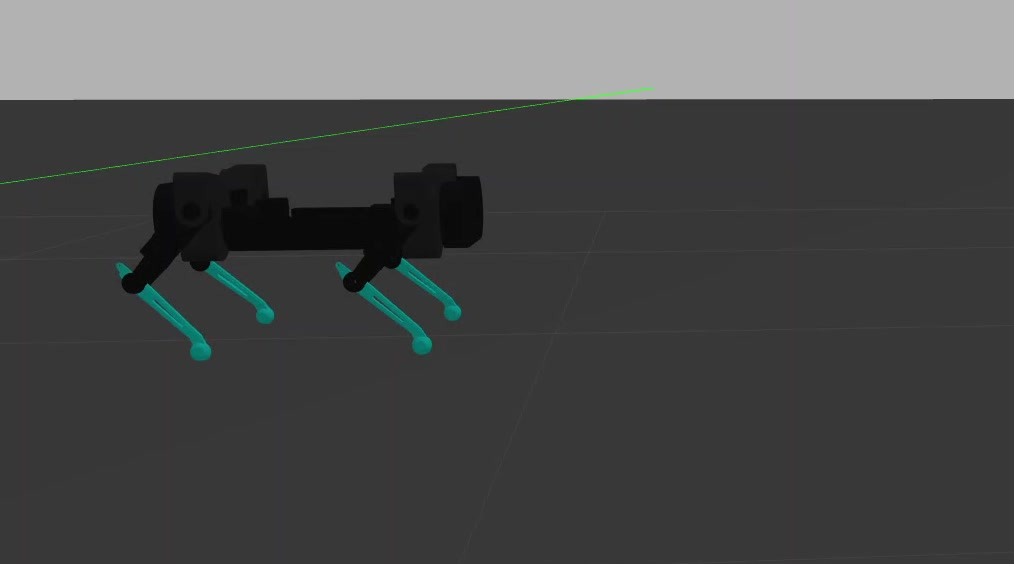
\includegraphics[width=\textwidth]{real_robot/gait/frames_cropped/30.jpg}
        \caption{$t=3.0$ s}
    \end{subfigure}
    \hfill
    \begin{subfigure}[b]{0.19\textwidth}
        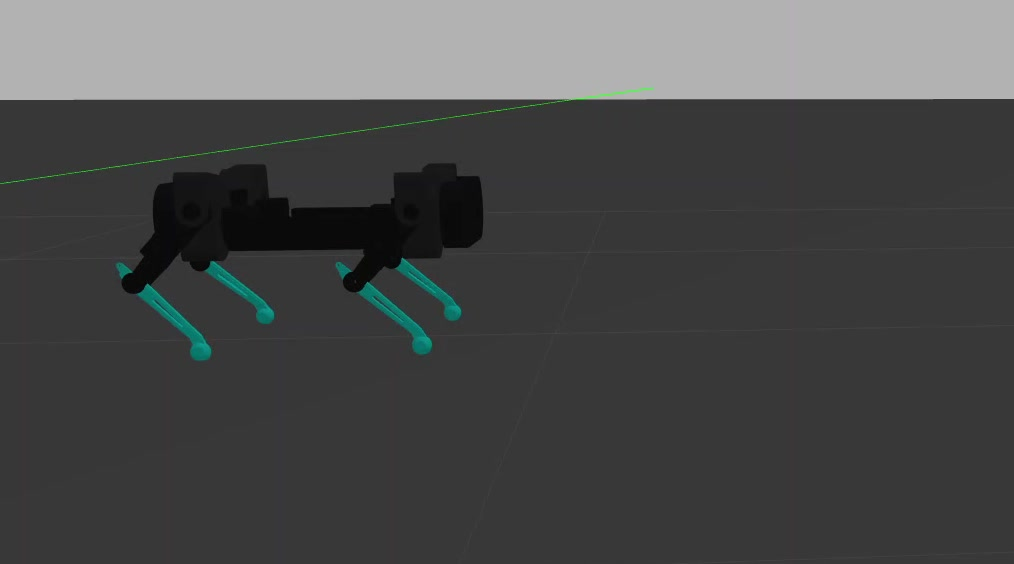
\includegraphics[width=\textwidth]{real_robot/gait/frames_cropped/40.jpg}
        \caption{$t=4.0$ s}
    \end{subfigure}
    \hfill
    \begin{subfigure}[b]{0.19\textwidth}
        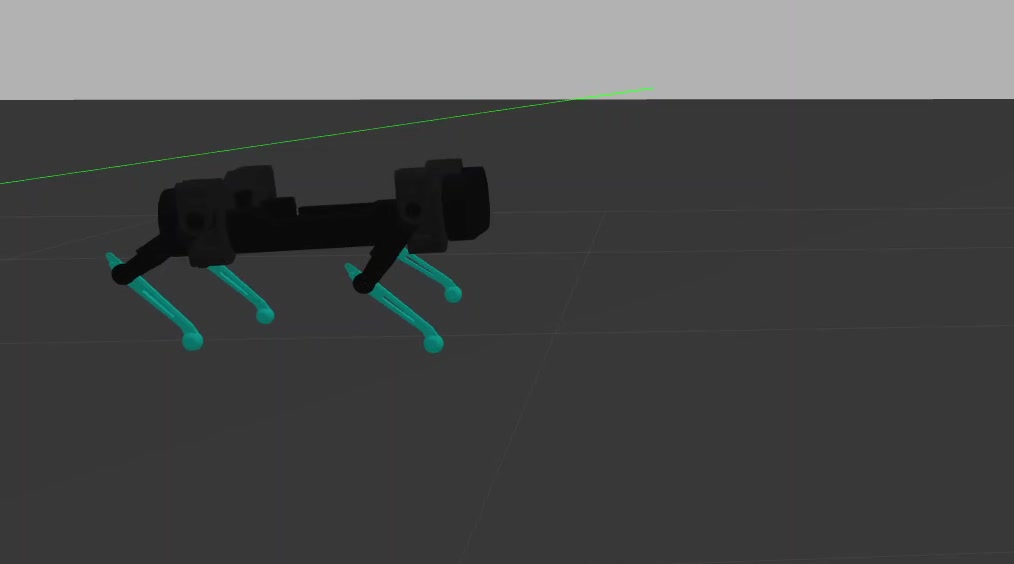
\includegraphics[width=\textwidth]{real_robot/gait/frames_cropped/50.jpg}
        \caption{$t=5.0$ s}
    \end{subfigure}
    \hfill
    \begin{subfigure}[b]{0.19\textwidth}
        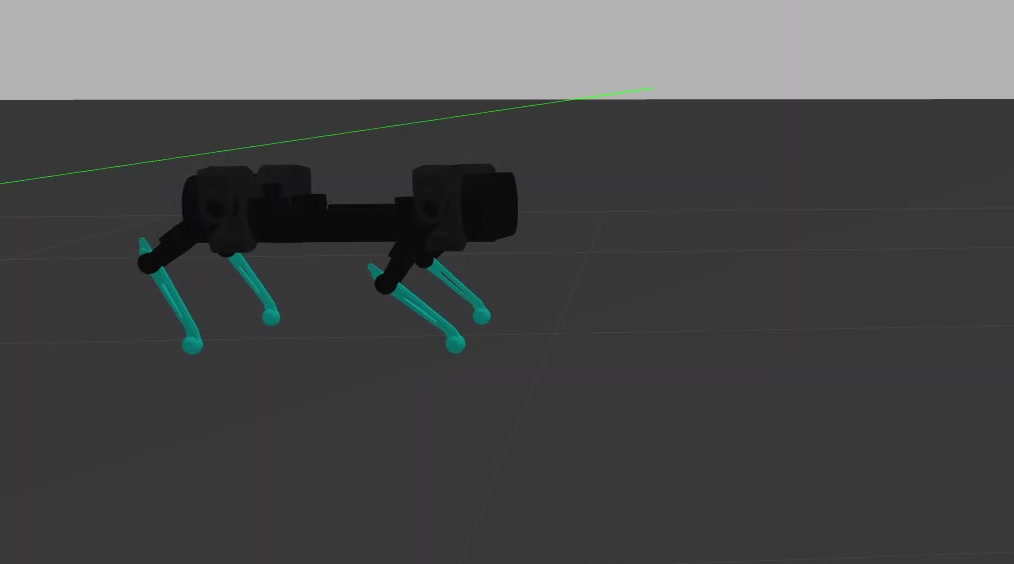
\includegraphics[width=\textwidth]{real_robot/gait/frames_cropped/60.jpg}
        \caption{$t=6.0$ s}
    \end{subfigure}
    
    \vspace{0.2cm}
    \begin{subfigure}[b]{0.19\textwidth}
        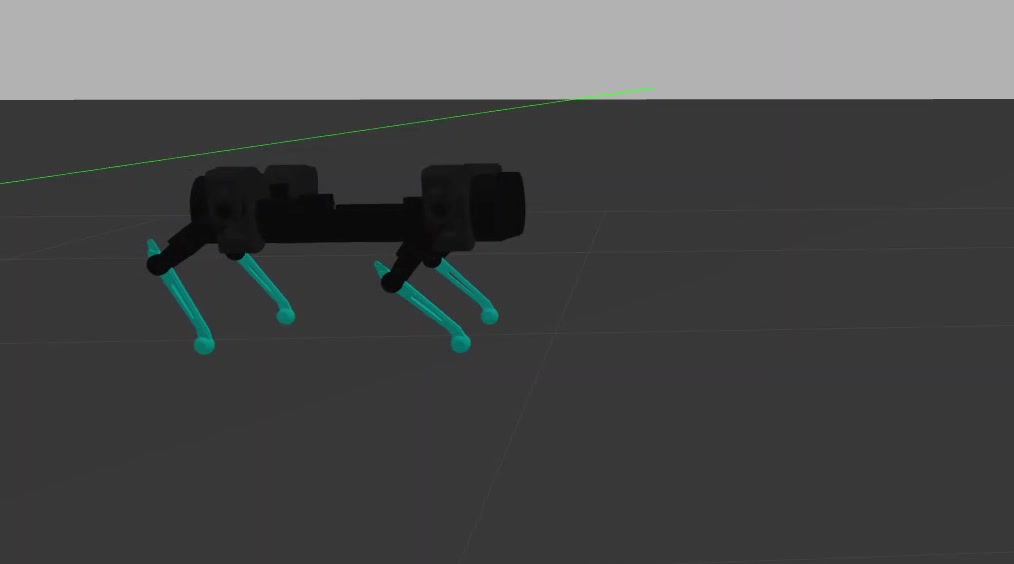
\includegraphics[width=\textwidth]{real_robot/gait/frames_cropped/70.jpg}
        \caption{$t=7.0$ s}
    \end{subfigure}
    \hfill
    \begin{subfigure}[b]{0.19\textwidth}
        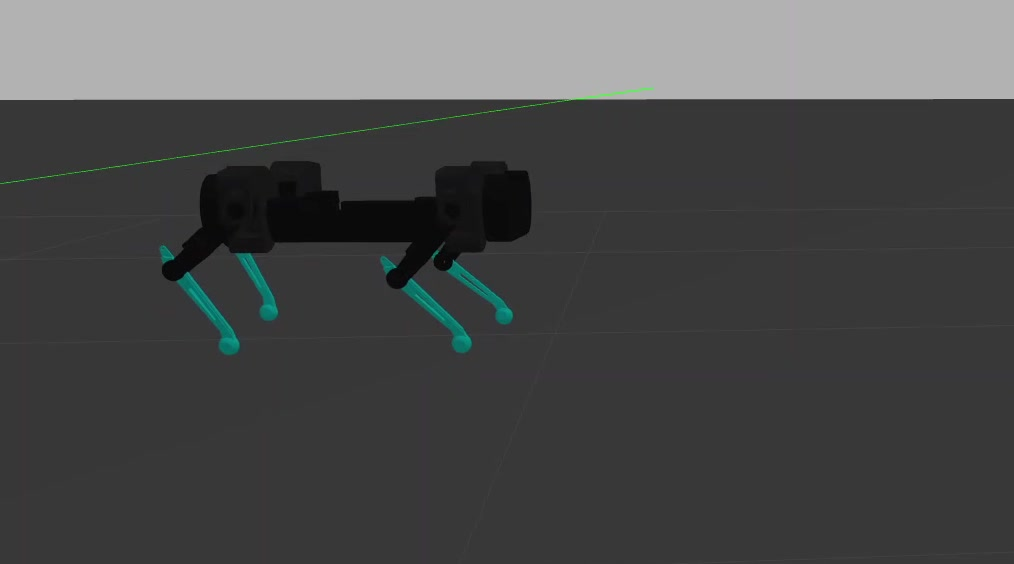
\includegraphics[width=\textwidth]{real_robot/gait/frames_cropped/80.jpg}
        \caption{$t=8.0$ s}
    \end{subfigure}
    \hfill
    \begin{subfigure}[b]{0.19\textwidth}
        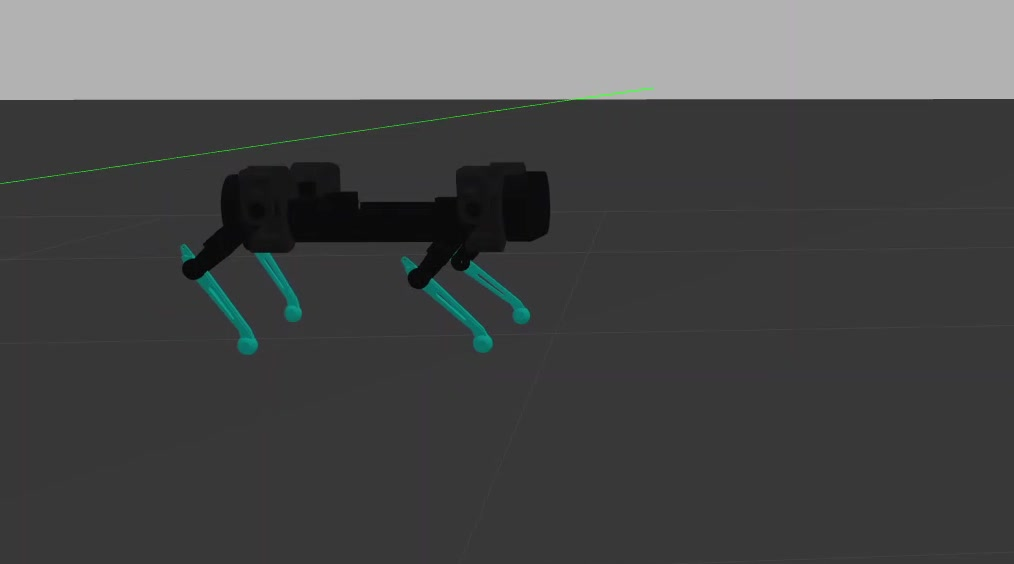
\includegraphics[width=\textwidth]{real_robot/gait/frames_cropped/90.jpg}
        \caption{$t=9.0$ s}
    \end{subfigure}
    \hfill
    \begin{subfigure}[b]{0.19\textwidth}
        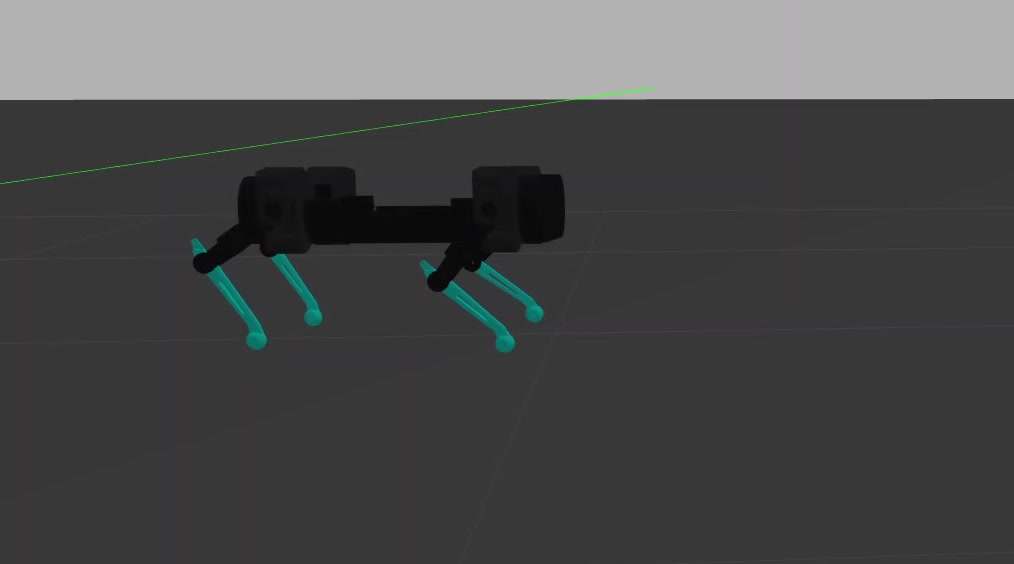
\includegraphics[width=\textwidth]{real_robot/gait/frames_cropped/100.jpg}
        \caption{$t=10.0$ s}
    \end{subfigure}
    \hfill
    \begin{subfigure}[b]{0.19\textwidth}
        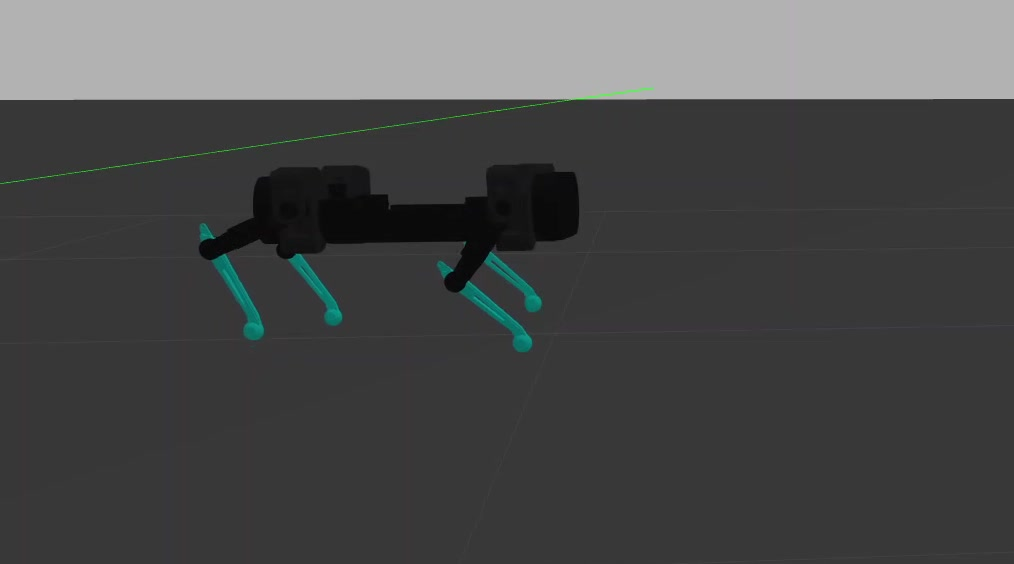
\includegraphics[width=\textwidth]{real_robot/gait/frames_cropped/110.jpg}
        \caption{$t=11.0$ s}
    \end{subfigure}
    \caption{Chuỗi chuyển động của robot trên hệ thống mô phỏng trong dáng đi Trot.}
    \label{fig:sim_trot_sequence}
\end{figure}



\section{Đánh giá hiệu năng bộ điều khiển PID nâng cao trên mô phỏng}

Phần này trình bày các kết quả thu được từ hệ thống mô phỏng, bao gồm dữ liệu chẩn đoán từ chuỗi xử lý PID và các biên dạng quỹ đạo offline. Bảng~\ref{tab:pid_home_params} và Bảng~\ref{tab:pid_gait_params} tổng hợp toàn bộ tham số điều khiển cho hai chế độ hoạt động, được trích xuất trực tiếp từ mã nguồn hệ thống.

\begin{table}[H]
\centering
\caption{Tham số bộ điều khiển PID -- Chế độ tĩnh (HOME)}
\label{tab:pid_home_params}
\renewcommand{\arraystretch}{1.3}
\begin{tabular}{|l|c|c|l|}
\hline
\textbf{Tham số} & \textbf{Ký hiệu} & \textbf{Giá trị} & \textbf{Mô tả} \\ \hline
Hệ số tỷ lệ & $K_P$ & 2,0 & Khuếch đại sai lệch \\ \hline
Hệ số tích phân & $K_I$ & 0,30 & Triệt tiêu sai số xác lập \\ \hline
Hệ số vi phân & $K_D$ & 0,15 & Giảm chấn dao động \\ \hline
Bão hòa đầu ra & $u_{max}$ & 1,5 rad & Giới hạn tín hiệu hiệu chỉnh \\ \hline
Bão hòa tích phân & $\mathcal{I}_{max}$ & 1,5 & Chống windup \\ \hline
Rò rỉ tích phân & $\lambda$ & 0,9995 & Hệ số decay \\ \hline
Vùng chết đo & $d$ & 0,02 rad & Triệt nhiễu nhỏ \\ \hline
Ngưỡng gain schedule & $e_{thresh}$ & 0,08 rad & Ngưỡng tỷ lệ khuếch đại \\ \hline
Hệ số LPF đầu vào & $\alpha_{raw}$ & 0,4 & Lọc EMA tín hiệu thô \\ \hline
Hệ số LPF đạo hàm & $\alpha_d$ & 0,7 & Lọc thành phần D \\ \hline
Hệ số LPF đầu ra & $\alpha_c$ & 0,15 & Làm mượt tín hiệu bù \\ \hline
\end{tabular}
\end{table}

\begin{table}[H]
\centering
\caption{Tham số bộ điều khiển PID -- Chế độ động (GAIT)}
\label{tab:pid_gait_params}
\renewcommand{\arraystretch}{1.3}
\begin{tabular}{|l|c|c|l|}
\hline
\textbf{Tham số} & \textbf{Ký hiệu} & \textbf{Giá trị} & \textbf{Mô tả} \\ \hline
Hệ số tỷ lệ & $K_P$ & 3,0 & Khuếch đại động \\ \hline
Hệ số tích phân & $K_I$ & 0,005 & Rất nhỏ (tránh dao động) \\ \hline
Hệ số vi phân & $K_D$ & 1,2 & Giảm chấn mạnh \\ \hline
Hệ số động P & $K_{prop}$ & 10,0 & Chia tỷ lệ dynamic gain \\ \hline
Vùng chết trung bình & $d_{avg}$ & 0,03 rad & Ngưỡng triệt nhiễu \\ \hline
Bão hòa đầu ra & $u_{max}$ & 0,30 rad & Giới hạn nhỏ hơn HOME \\ \hline
Bão hòa tích phân & $\mathcal{I}_{max}$ & 0,3 & Chống windup \\ \hline
Hệ số LPF đầu ra & $\alpha_{lpf}$ & 0,97 & Lọc mạnh hơn HOME \\ \hline
Số chu kỳ học baseline & $N_{learn}$ & 2 & Chu kỳ dáng đi \\ \hline
Tốc độ hội tụ baseline & $\eta_{adapt}$ & 0,05 & Cập nhật baseline \\ \hline
\end{tabular}
\end{table}

Sự khác biệt giữa hai bộ tham số phản ánh yêu cầu vận hành riêng biệt: chế độ HOME cần phản ứng nhanh ($K_P = 2{,}0$, $\alpha_c = 0{,}15$) để bù nhiễu loạn tức thời, trong khi chế độ GAIT cần lọc mạnh ($\alpha_{lpf} = 0{,}97$) và giới hạn đầu ra nhỏ ($u_{max} = 0{,}30$ rad) để tránh can thiệp quá mức vào quỹ đạo sải bước.

\subsection{Kết quả quy hoạch quỹ đạo offline}

Hình~\ref{results/offline_traj_pos} trình bày quỹ đạo Cartesian $(x, y, z)$ của chân trước bên trái (Left-Front) trong một chu kỳ dáng đi đầy đủ. Việc quy hoạch quỹ đạo trục $z$ theo biên dạng parabol với độ cao $h_{lift} = 80$ mm là đặc biệt quan trọng để tạo ra hình dáng chữ D (D-shape trajectory). Thiết kế này giải quyết bài toán tránh va chạm (ground clearance), giúp chân robot không bị vấp phải các chướng ngại vật nhỏ trên mặt đất khi vung chân. Đồng thời, việc trục $y$ được duy trì ổn định tại giá trị $0$ mang ý nghĩa đảm bảo chân bước thẳng, loại bỏ hoàn toàn hiện tượng trượt ngang (slippage) -- nguyên nhân chính gây hao hụt động năng và làm suy giảm khả năng định hướng khi robot di chuyển.

\begin{figure}[H]
    \centering
    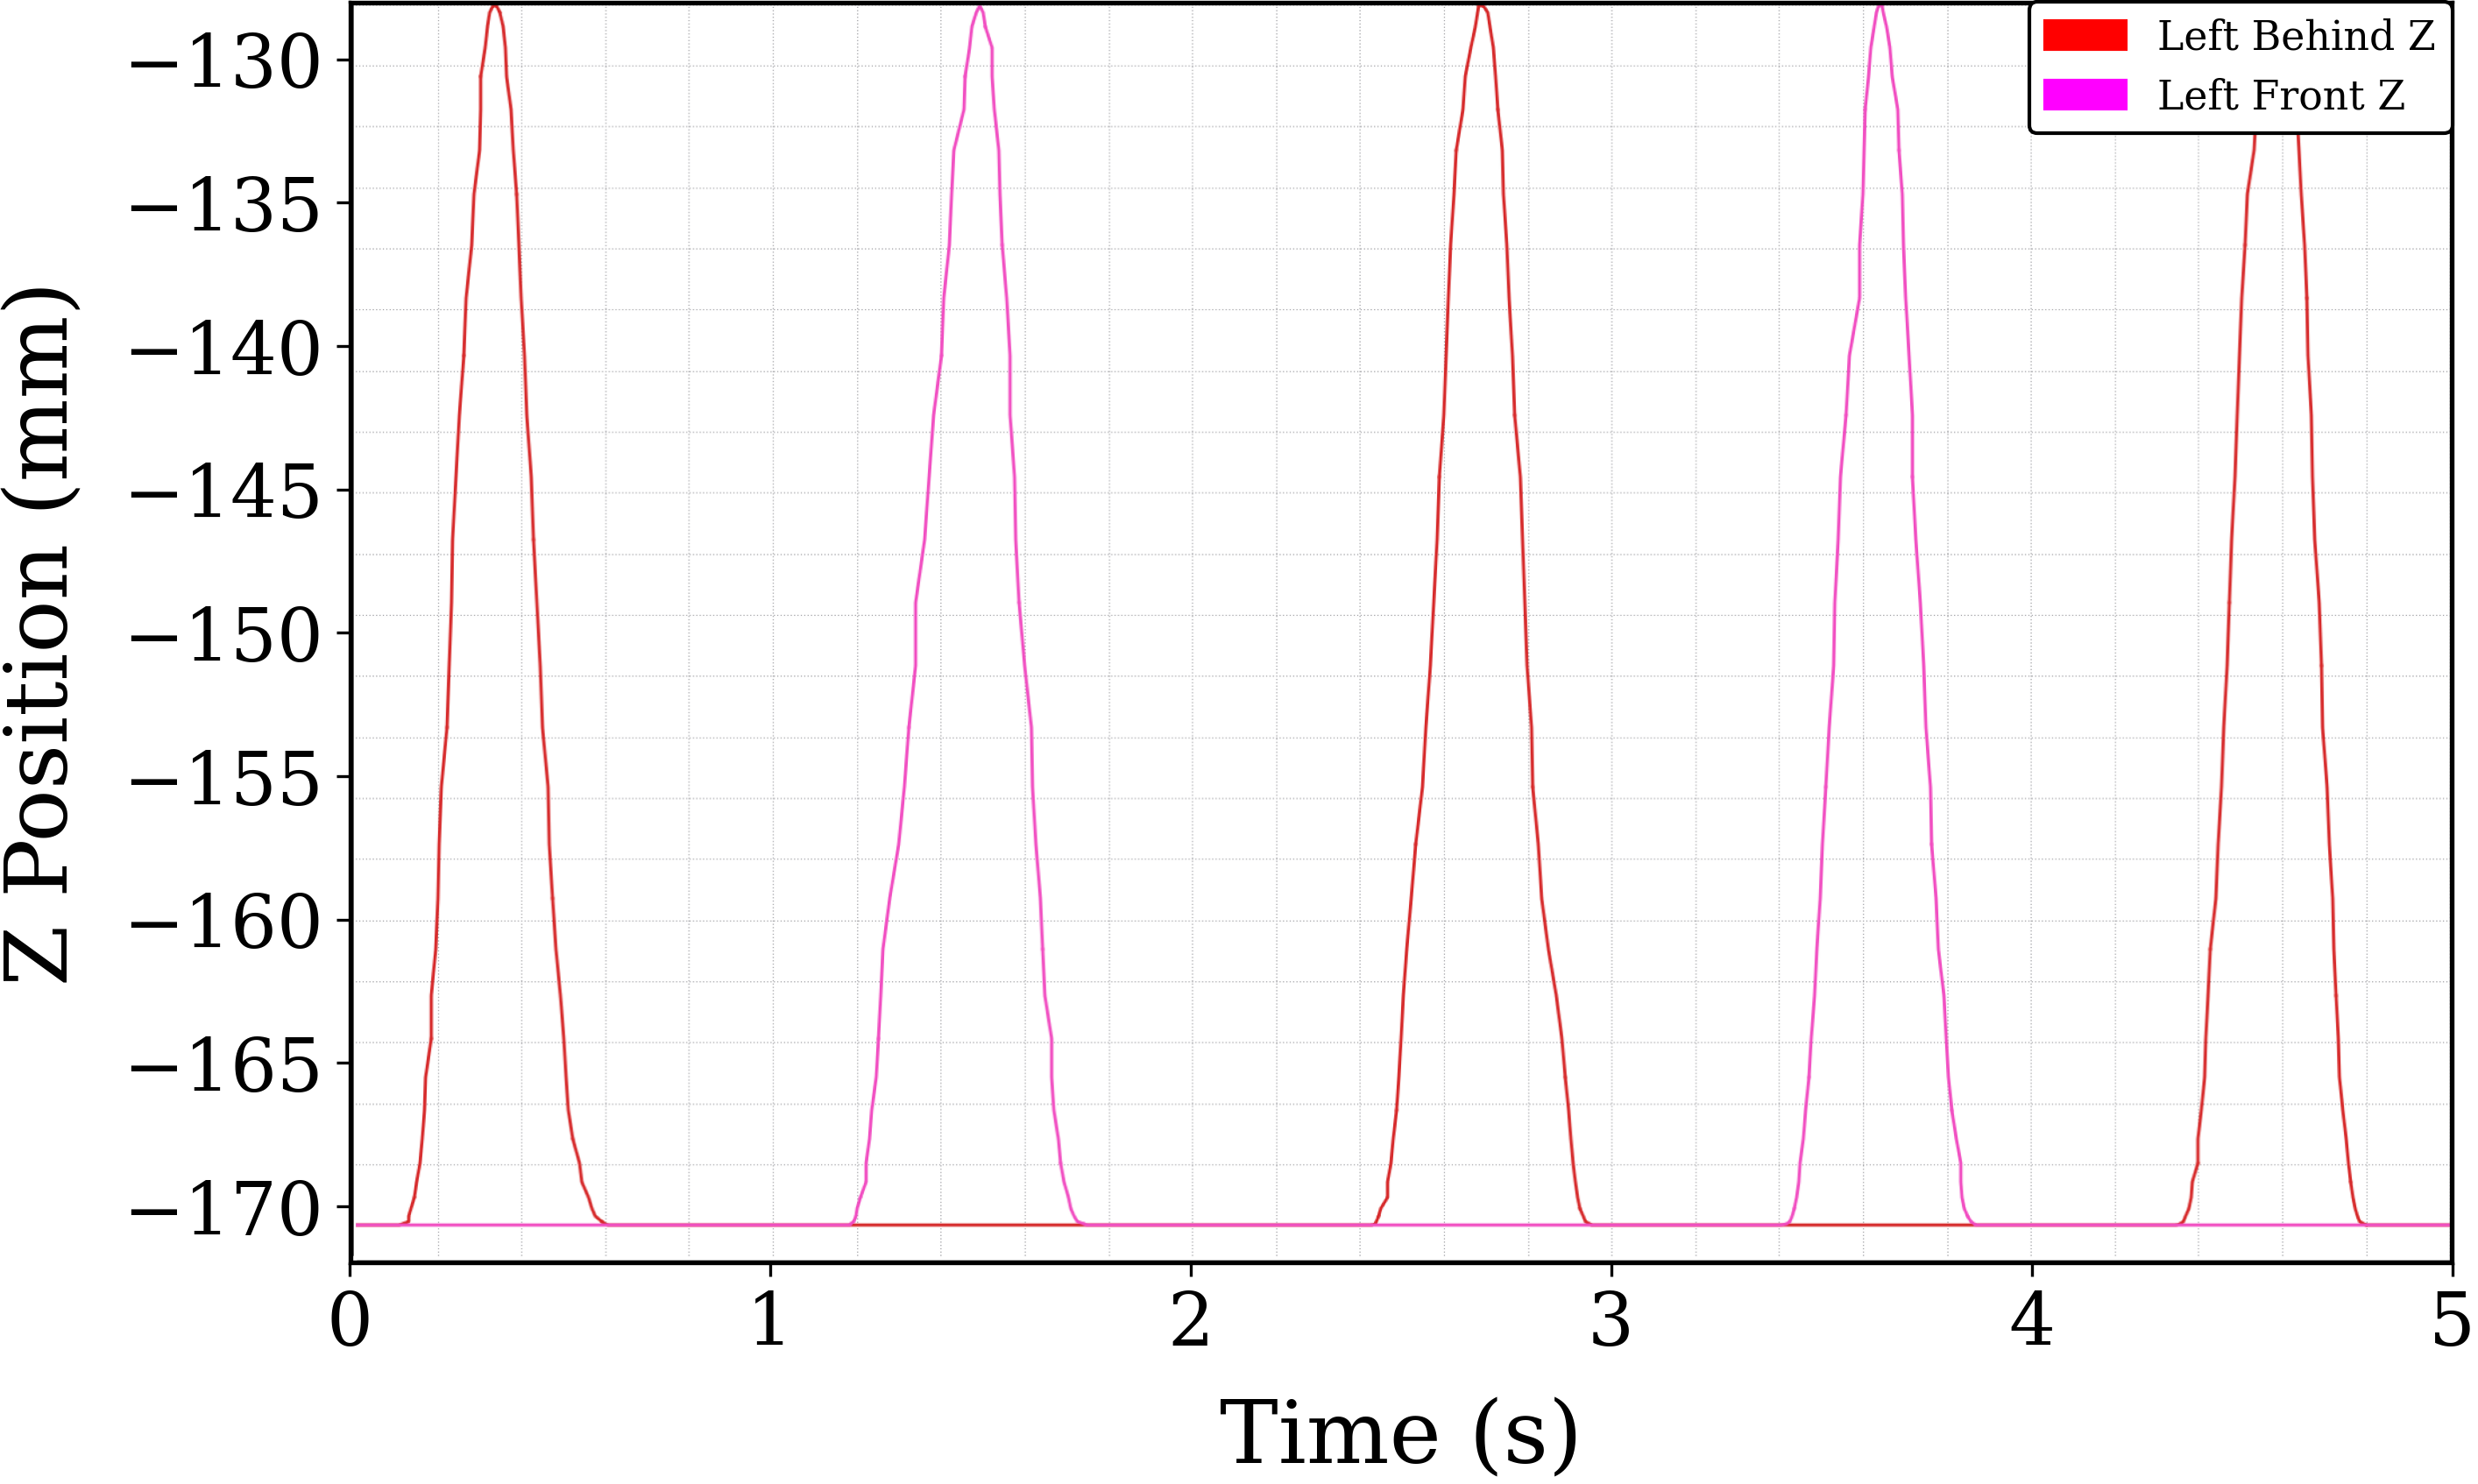
\includegraphics[width=0.8\textwidth]{results/offline_traj_pos.png}
    \caption{Quỹ đạo Cartesian $(x, y, z)$ của chân trước bên trái trong một chu kỳ dáng đi}
    \label{results/offline_traj_pos}
\end{figure}

Hình~\ref{results/offline_traj_vel_acc} trình bày biên dạng vận tốc và gia tốc của quỹ đạo. Kết quả này không chỉ xác nhận tính đúng đắn về mặt toán học mà còn mang ý nghĩa cơ khí thiết thực: việc đáp ứng được các điều kiện biên $\dot{s}(0) = \dot{s}(1) = 0$ và $\ddot{s}(0) = \ddot{s}(1) = 0$ của hàm đa thức bậc 5 (quintic) giúp triệt tiêu hoàn toàn sự thay đổi gia tốc đột ngột (infinite jerk). Phương pháp này giải quyết bài toán chống sốc cơ học tại hai thời điểm nhạy cảm nhất là nhấc chân (lift-off) và chạm đất (touch-down), từ đó giảm thiểu hao mòn bánh răng và kéo dài tuổi thọ của các động cơ servo.

\begin{figure}[H]
    \centering
    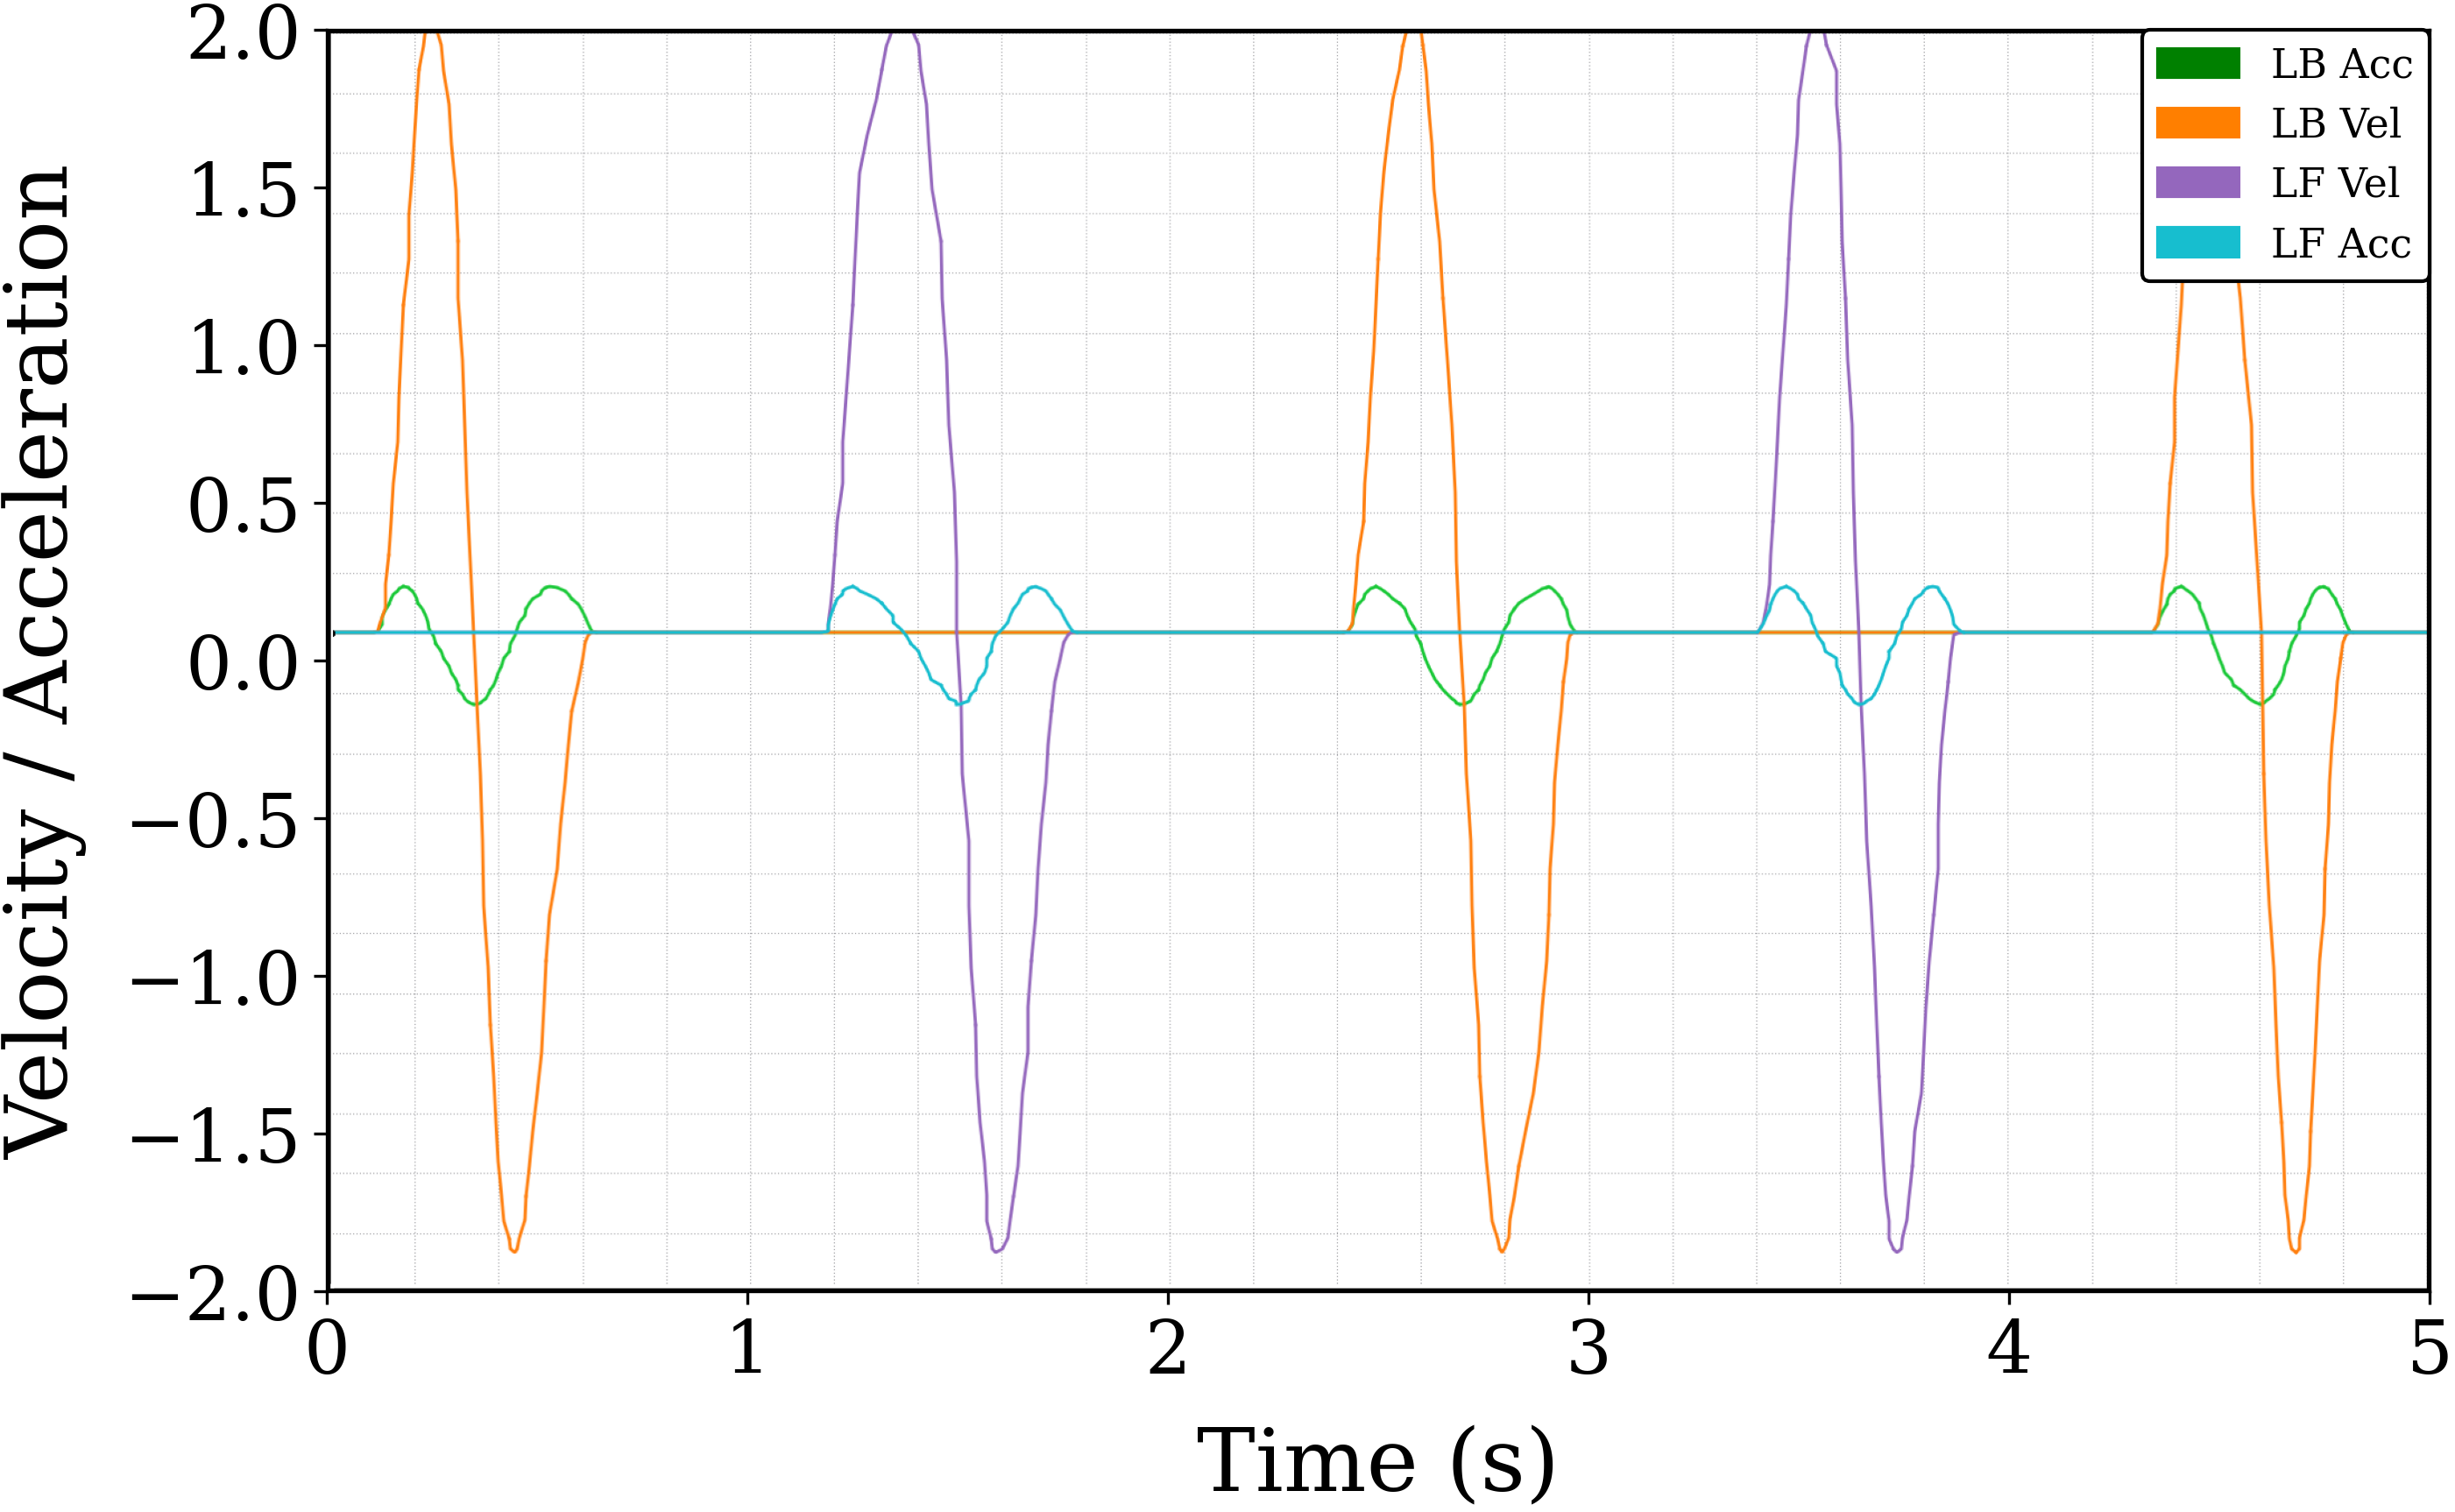
\includegraphics[width=0.8\textwidth]{results/offline_traj_vel_acc.png}
    \caption{Biên dạng vận tốc và gia tốc của chân trước bên trái}
    \label{results/offline_traj_vel_acc}
\end{figure}

Hình~\ref{results/offline_traj_angle} cho thấy các góc khớp $(\theta_1, \theta_2, \theta_3)$ thu được từ bộ giải động học nghịch (IK). Tính trơn tru, liên tục và không xuất hiện các đỉnh nhọn (bước nhảy) trong đồ thị này có ý nghĩa khẳng định rằng bộ tham số không gian cấu hình ($L_{stride}=10$ mm, $h_{lift}=80$ mm) được chọn nằm hoàn toàn bên trong vùng không gian làm việc an toàn (reachable workspace) của robot. Điều này chứng minh thuật toán IK đã giải quyết thành công bài toán nội suy tọa độ mà không vướng phải các điểm kỳ dị (singularities).

\begin{figure}[H]
    \centering
    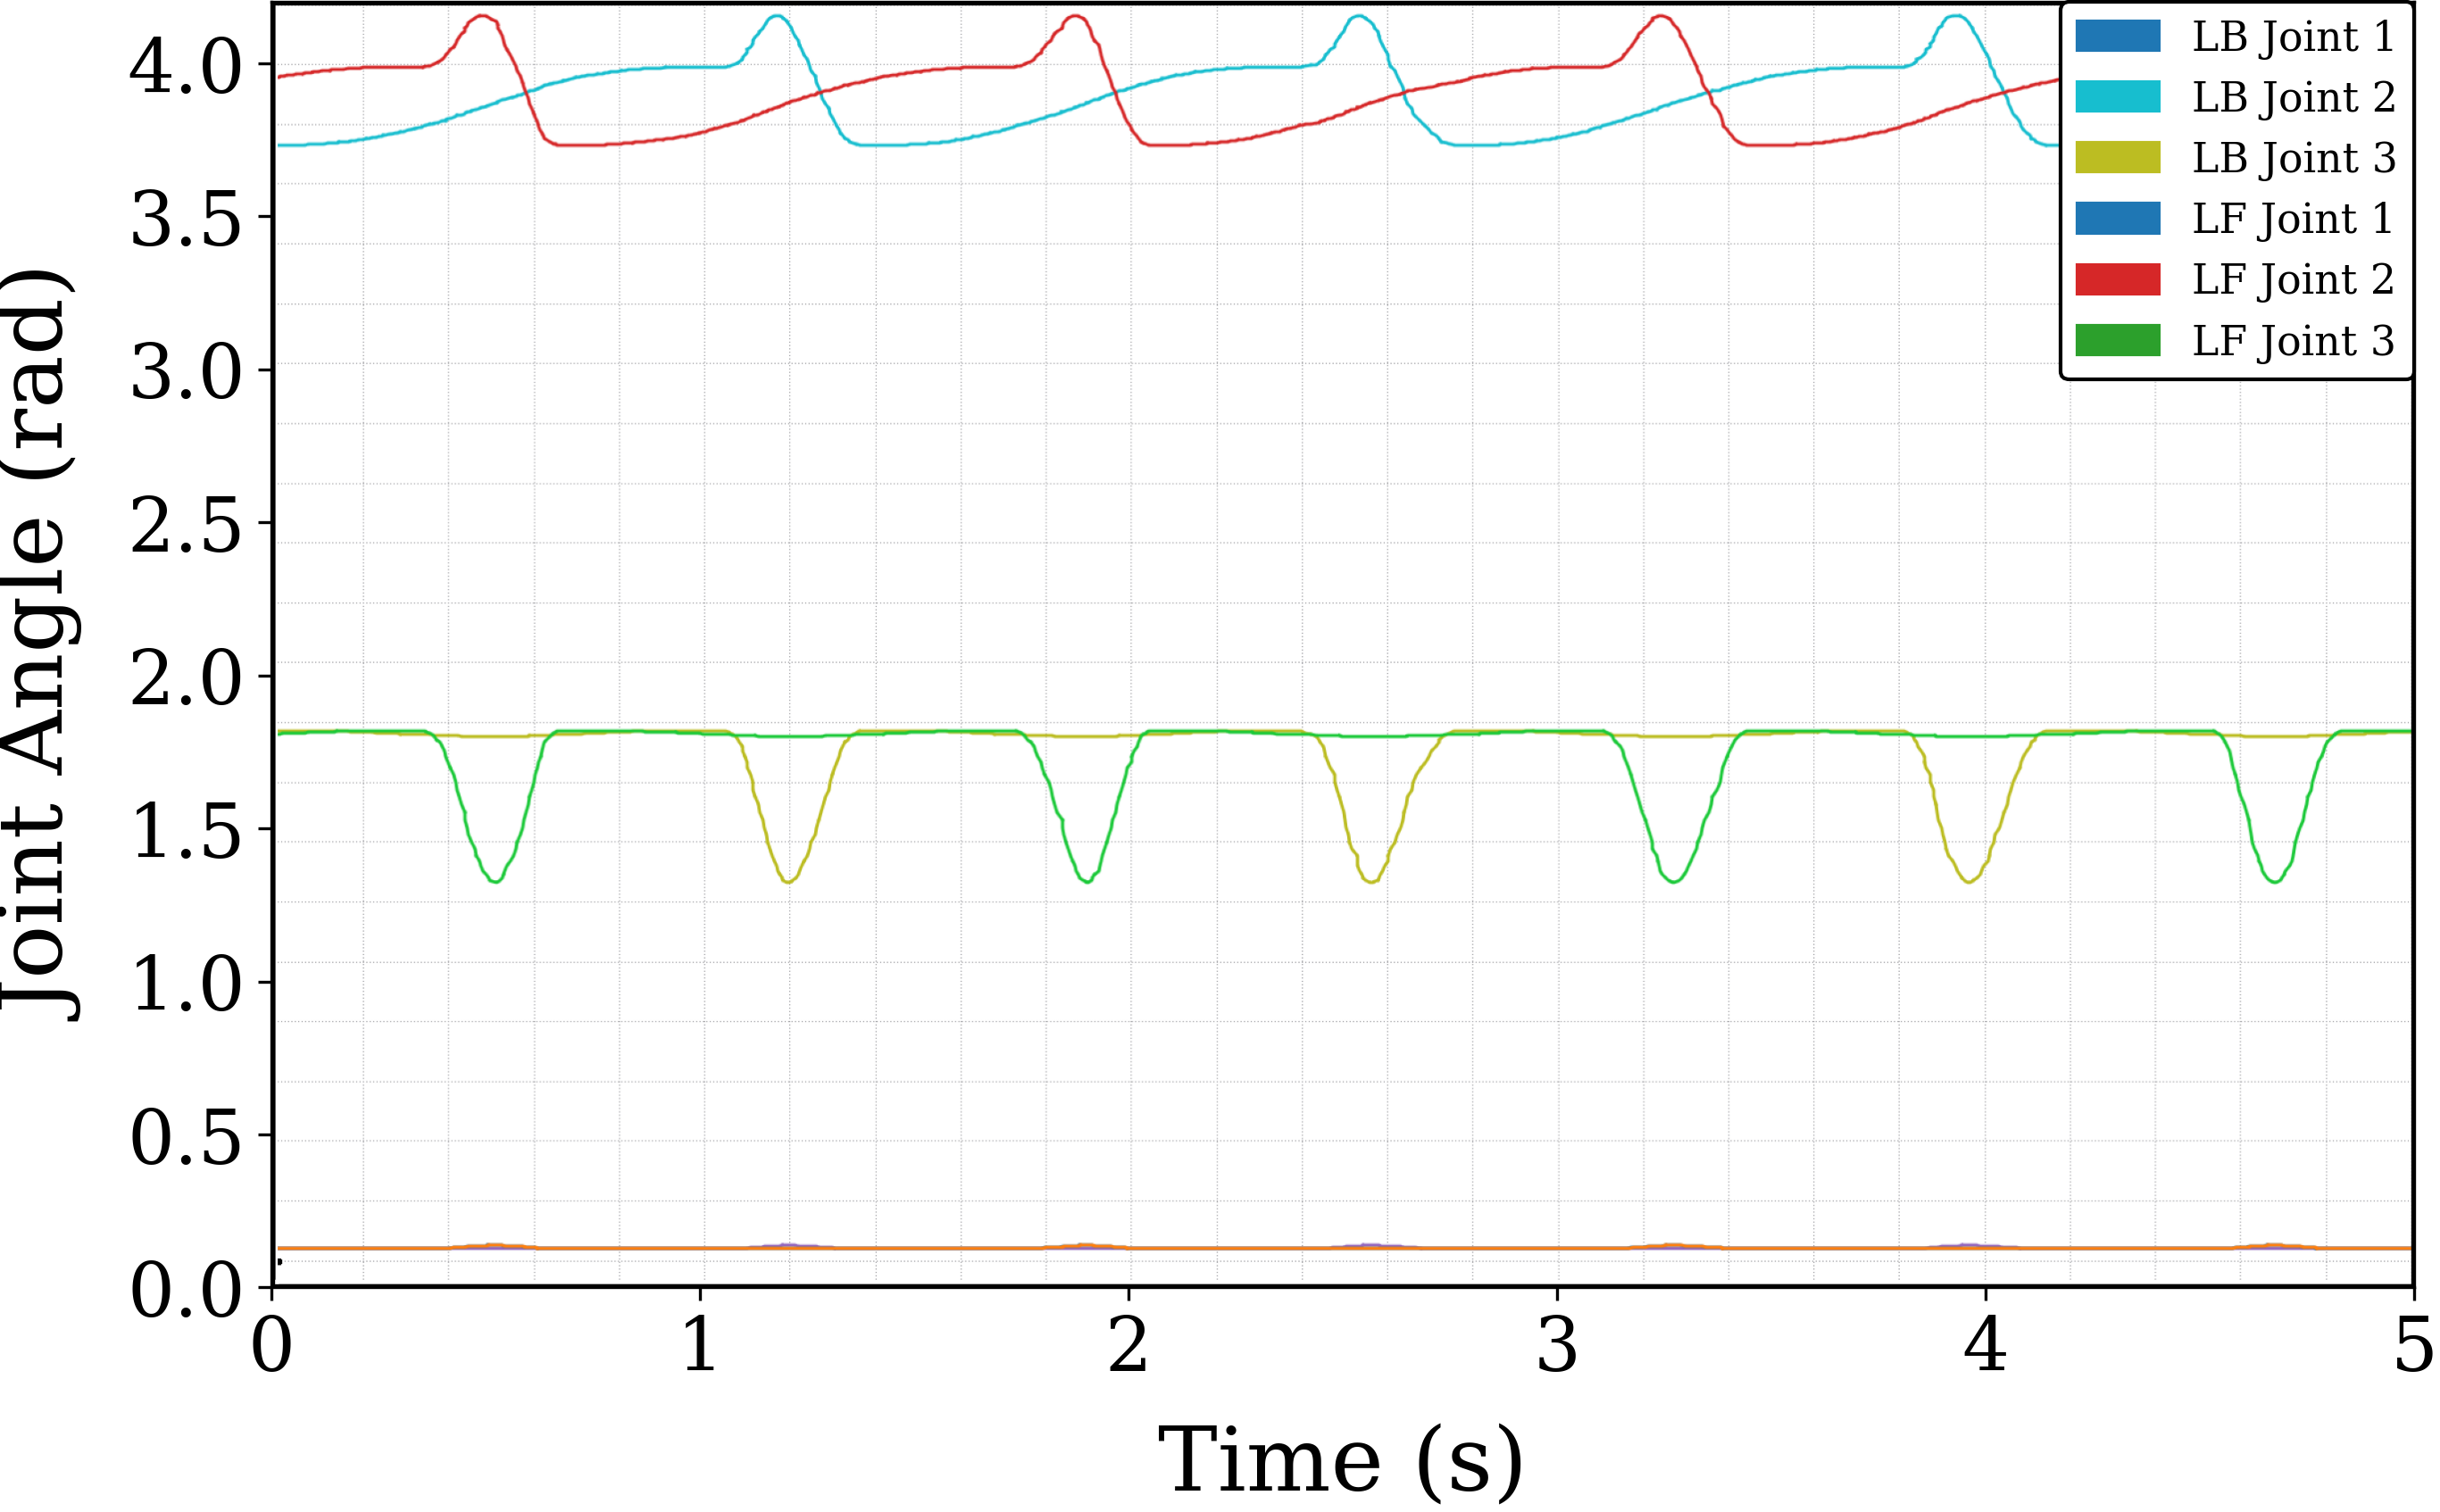
\includegraphics[width=0.8\textwidth]{results/offline_traj_angle.png}
    \caption{Góc khớp $(\theta_1, \theta_2, \theta_3)$ giải qua IK cho các chân bên trái (LF và LB)}
    \label{results/offline_traj_angle}
\end{figure}

\subsection{Quỹ đạo 3D bàn chân trong môi trường mô phỏng}

Hình~\ref{fig_gait_3d_real} trình bày quỹ đạo 3D thực tế của bàn chân khi chạy trong môi trường mô phỏng Gazebo. Ý nghĩa của đồ thị này vượt ra ngoài việc xác nhận hình chữ D đặc trưng; nó minh chứng cho sự tương thích hoàn hảo giữa luồng phần mềm lập kế hoạch tĩnh (ROS~2 node) và Engine vật lý động lực học (chịu ảnh hưởng của trọng lực, ma sát, quán tính). Quỹ đạo thực tế bám sát quỹ đạo lý thuyết chứng minh rằng bộ điều khiển cấp thấp (Low-level PD controller) trên mô phỏng đã giải quyết tốt bài toán thực thi quỹ đạo dưới tải trọng ảo của robot.

\begin{figure}[H]
    \centering
    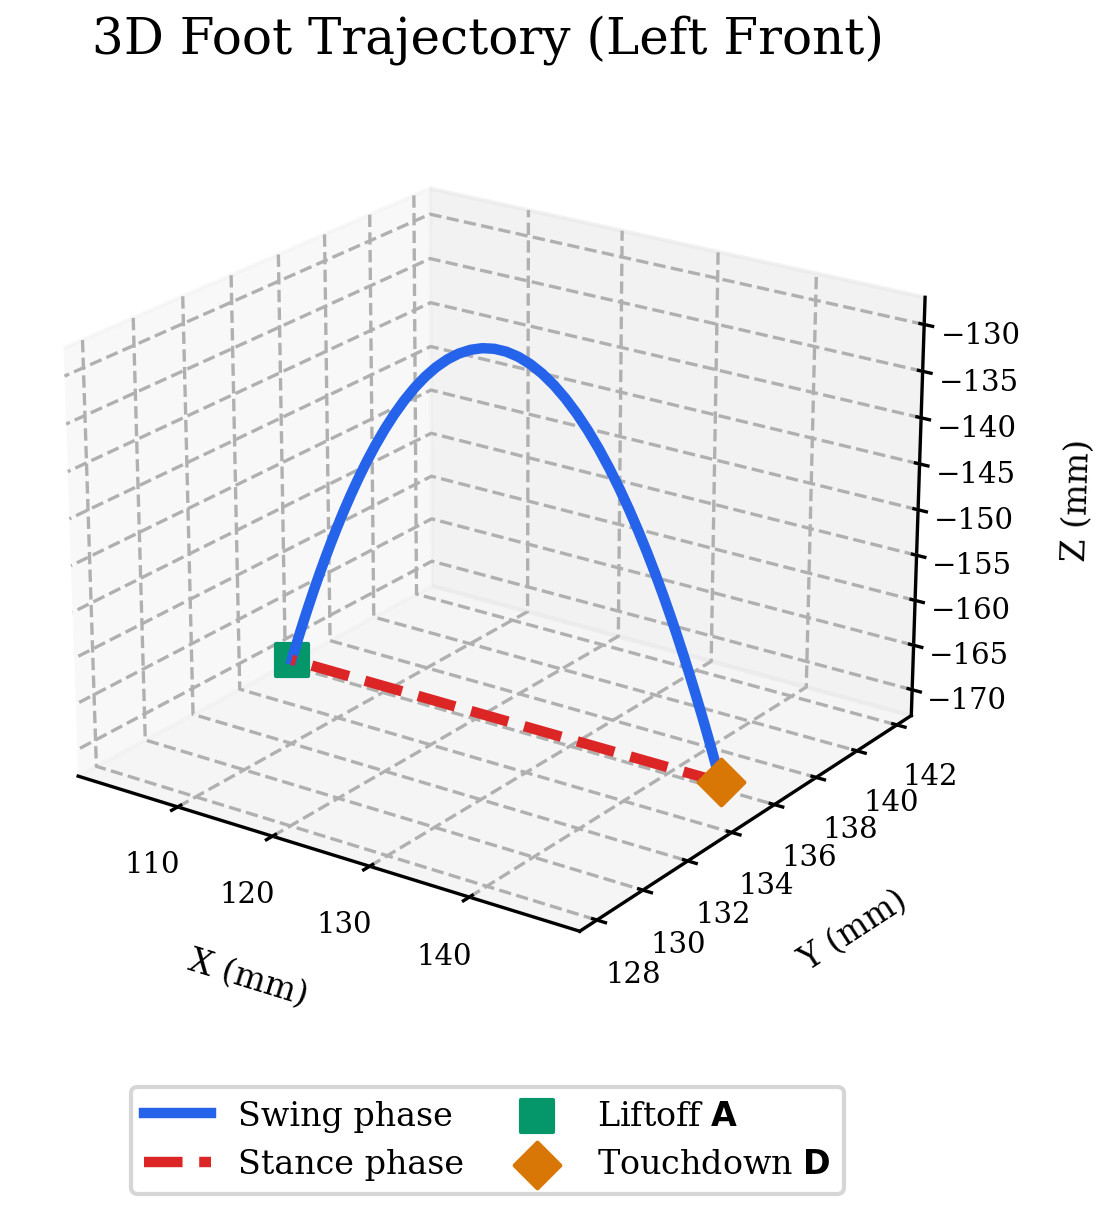
\includegraphics[width=0.6\textwidth]{gait_planner/gait_3d.png}
    \caption{Quỹ đạo 3D bàn chân chân trước bên trái trên hệ thống mô phỏng}
    \label{fig_gait_3d_real}
\end{figure}

\subsection{Ổn định tư thế tĩnh (chế độ HOME)}

Hình~\ref{fig_pid_home} trình bày khả năng duy trì thăng bằng của hệ thống vòng kín PID trong chế độ HOME khi chịu tác động của mặt phẳng dao động lượn sóng liên tục (biên độ nhiễu $\approx 10^\circ$). Đồ thị này mang ý nghĩa minh chứng cho sự ưu việt của cơ cấu xử lý phi tuyến: thay vì cố gắng đưa sai lệch (Error) về tuyệt đối bằng 0 --- một việc thường dẫn đến hiện tượng động cơ nhích liên tục gây ồn và quá nhiệt (chattering) --- hệ thống chủ động áp dụng vùng chết (deadband $\pm 0{,}02$ rad). Đặc điểm "cắt phẳng" của đồ thị Error quanh trục hoành chứng tỏ thuật toán đã giải quyết thành công bài toán đánh đổi giữa độ chính xác và năng lượng tiêu thụ; robot chấp nhận một sai số vi mô không thể nhận biết bằng mắt thường để đổi lấy sự tĩnh lặng tuyệt đối của cơ khí. Thêm vào đó, khi nhiễu đổi chiều đột ngột, cơ chế chống bão hòa khâu tích phân (Anti-windup) bảo vệ hệ thống khỏi hiện tượng văng lố (overshoot), đảm bảo tư thế robot luôn êm ái.

\begin{figure}[H]
    \centering
    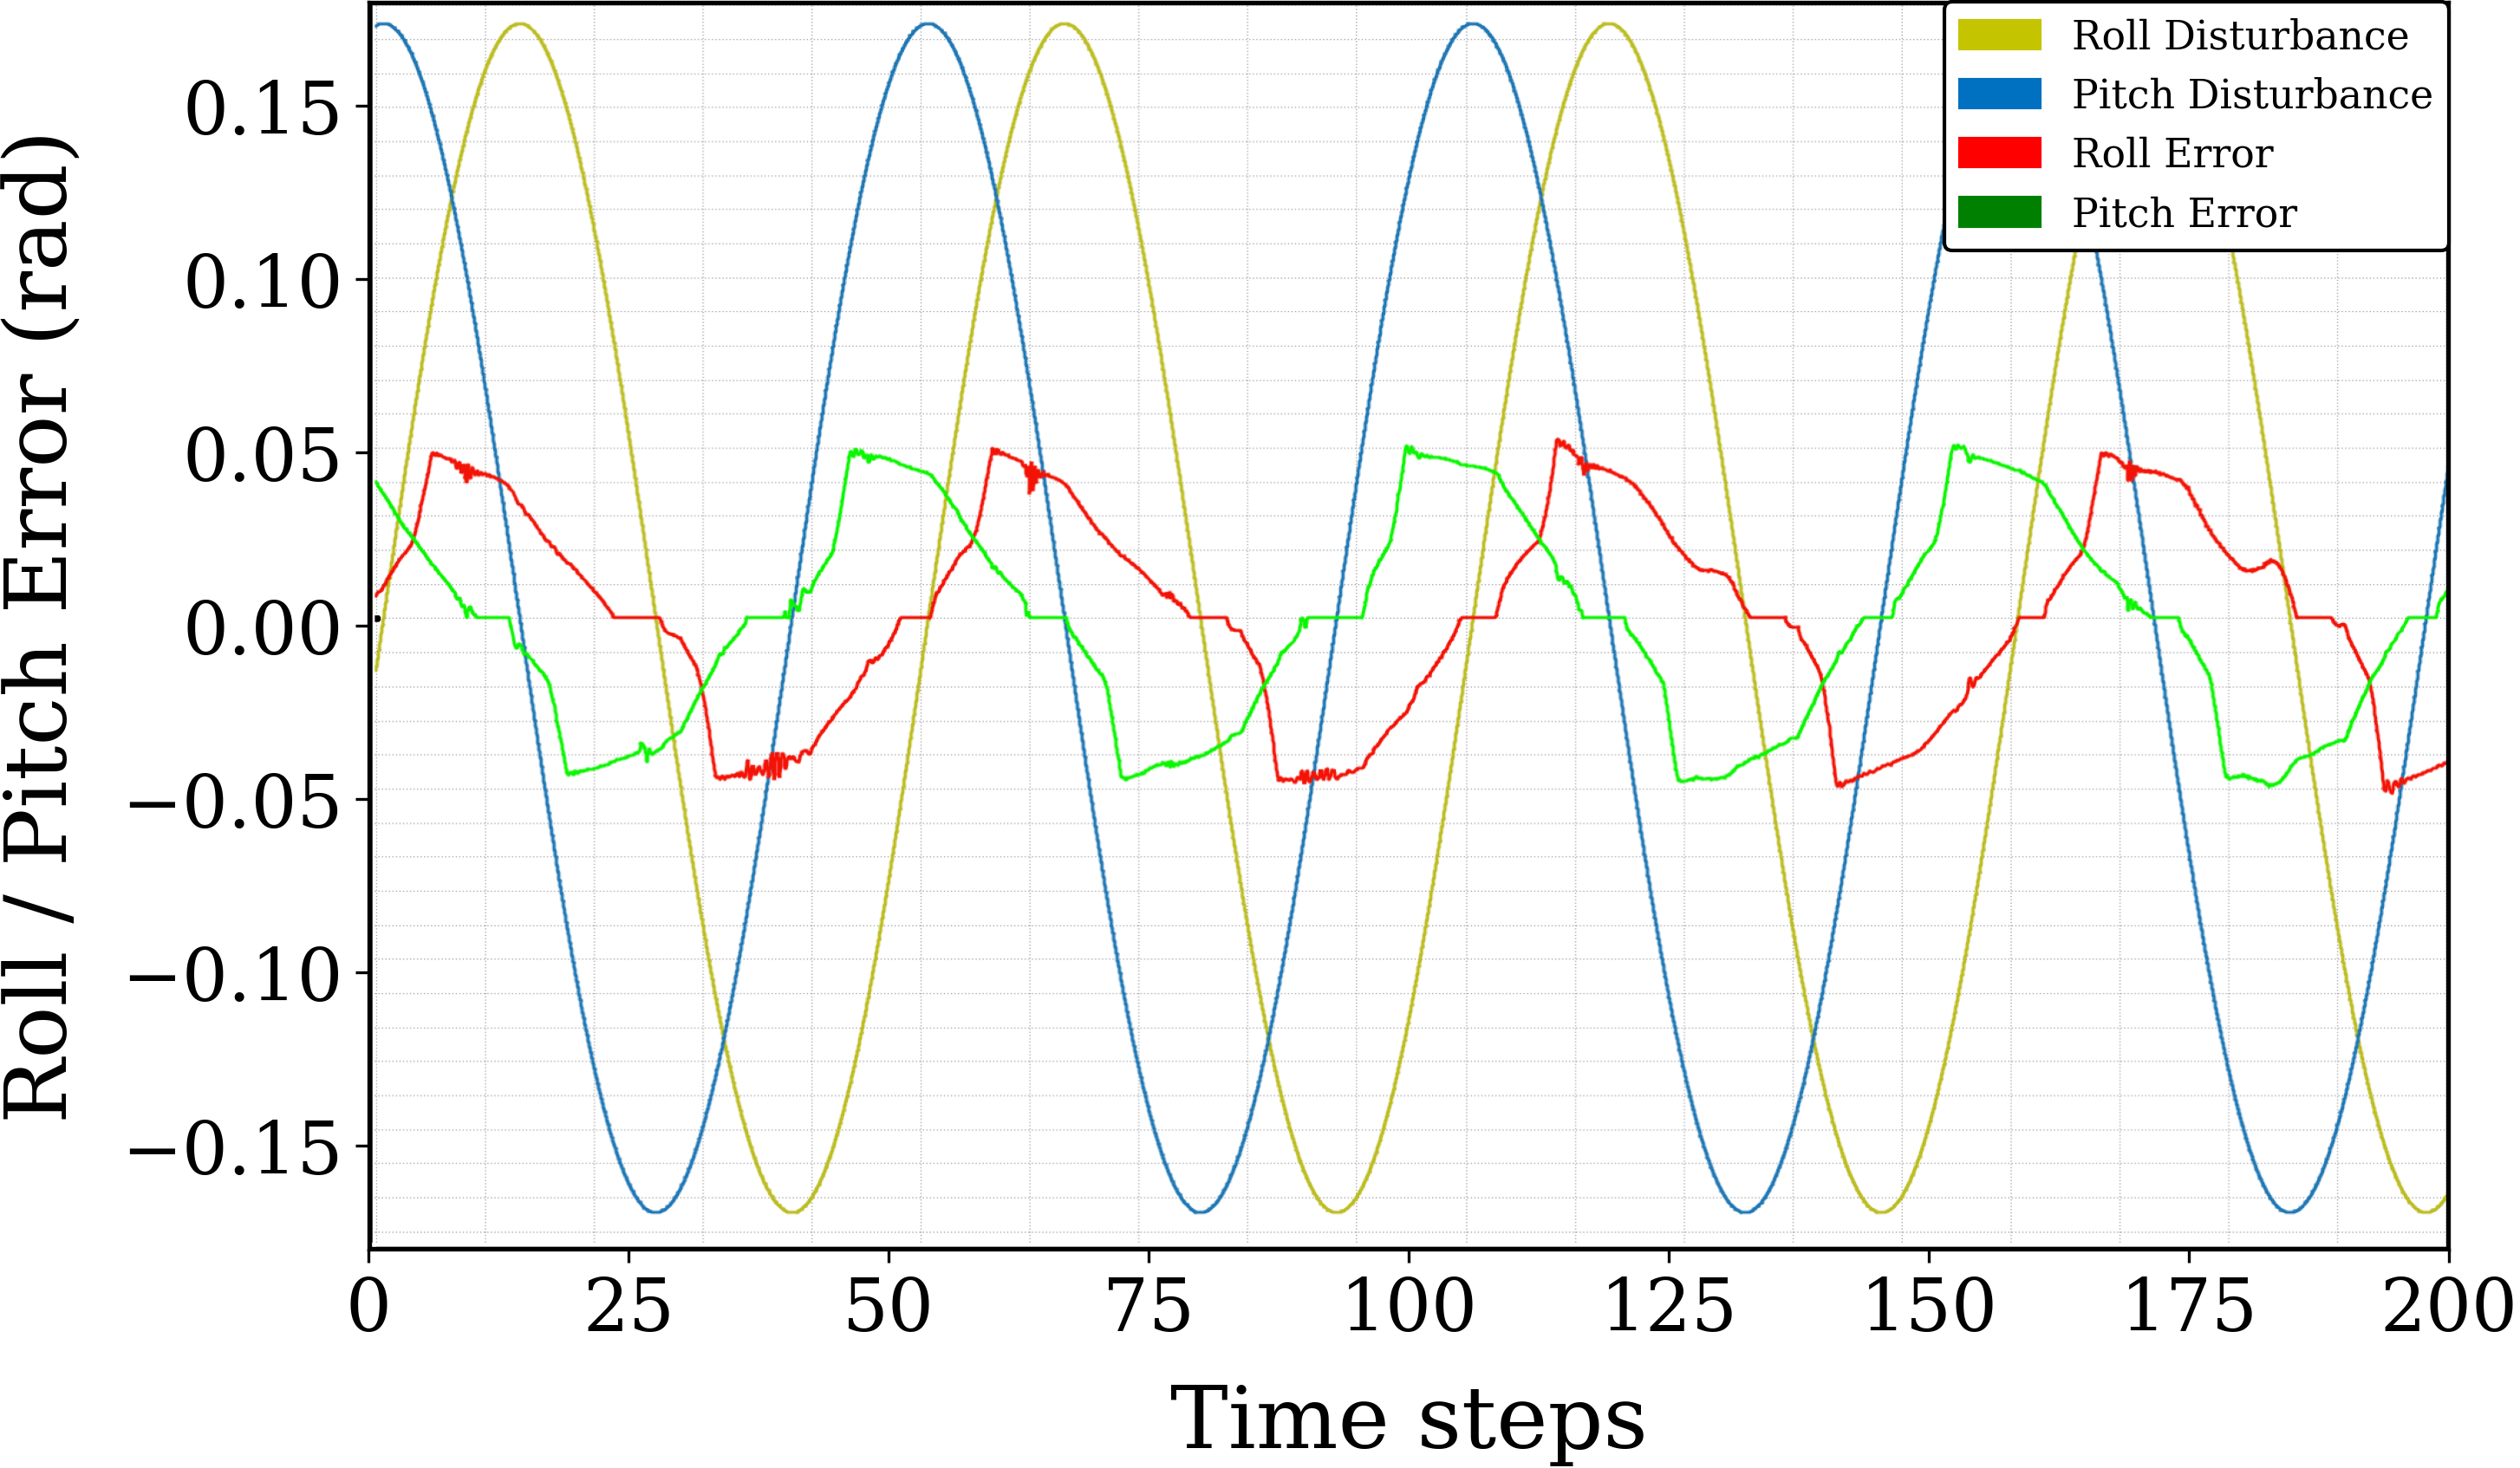
\includegraphics[width=0.85\textwidth]{results/pid_error_home.png}
    \caption{Đáp ứng sai lệch bộ điều khiển trong chế độ tĩnh HOME}
    \label{fig_pid_home}
\end{figure}

\subsubsection*{Phân tích tín hiệu nội bộ chuỗi xử lý PID (Chế độ HOME)}

Dựa trên kiến trúc điều khiển đã đề xuất ở Chương 2, hiệu năng của từng khối xử lý tín hiệu trong bộ điều khiển Roll và Pitch được đánh giá chi tiết thông qua các tín hiệu nội bộ thu thập từ mô phỏng. 

Hình \ref{fig:home_pid_roll_meas} và Hình \ref{fig:home_pid_pitch_meas} giải thích lý do tại sao tín hiệu thô không thể được đưa trực tiếp vào vòng lặp điều khiển. Cảm biến IMU gắn trên khung gầm robot vốn luôn bị ảnh hưởng bởi nhiễu rung động cơ học (mechanical vibration) từ các động cơ. Nếu không có bộ lọc trung bình trượt hàm mũ (EMA), khâu vi phân của PID sẽ khuếch đại các nhiễu tần số cao này thành những lệnh bù giật cục. Tại đầu ra, việc áp dụng khâu bão hòa (giới hạn ở $\pm 1{,}5$ rad) và bộ lọc thông thấp (LPF) giải quyết rủi ro mất an toàn: cơ cấu này ngăn chặn việc xuất ra các góc bù lớn đột biến có thể làm bật ngửa thân robot, đồng thời vuốt mượt tín hiệu bù (đường LPF trong đồ thị trơn hơn hẳn đường Sat) để các khớp gối phản hồi một cách uyển chuyển.

\begin{figure}[H]
    \centering
    \begin{subfigure}[b]{0.48\textwidth}
        \centering
        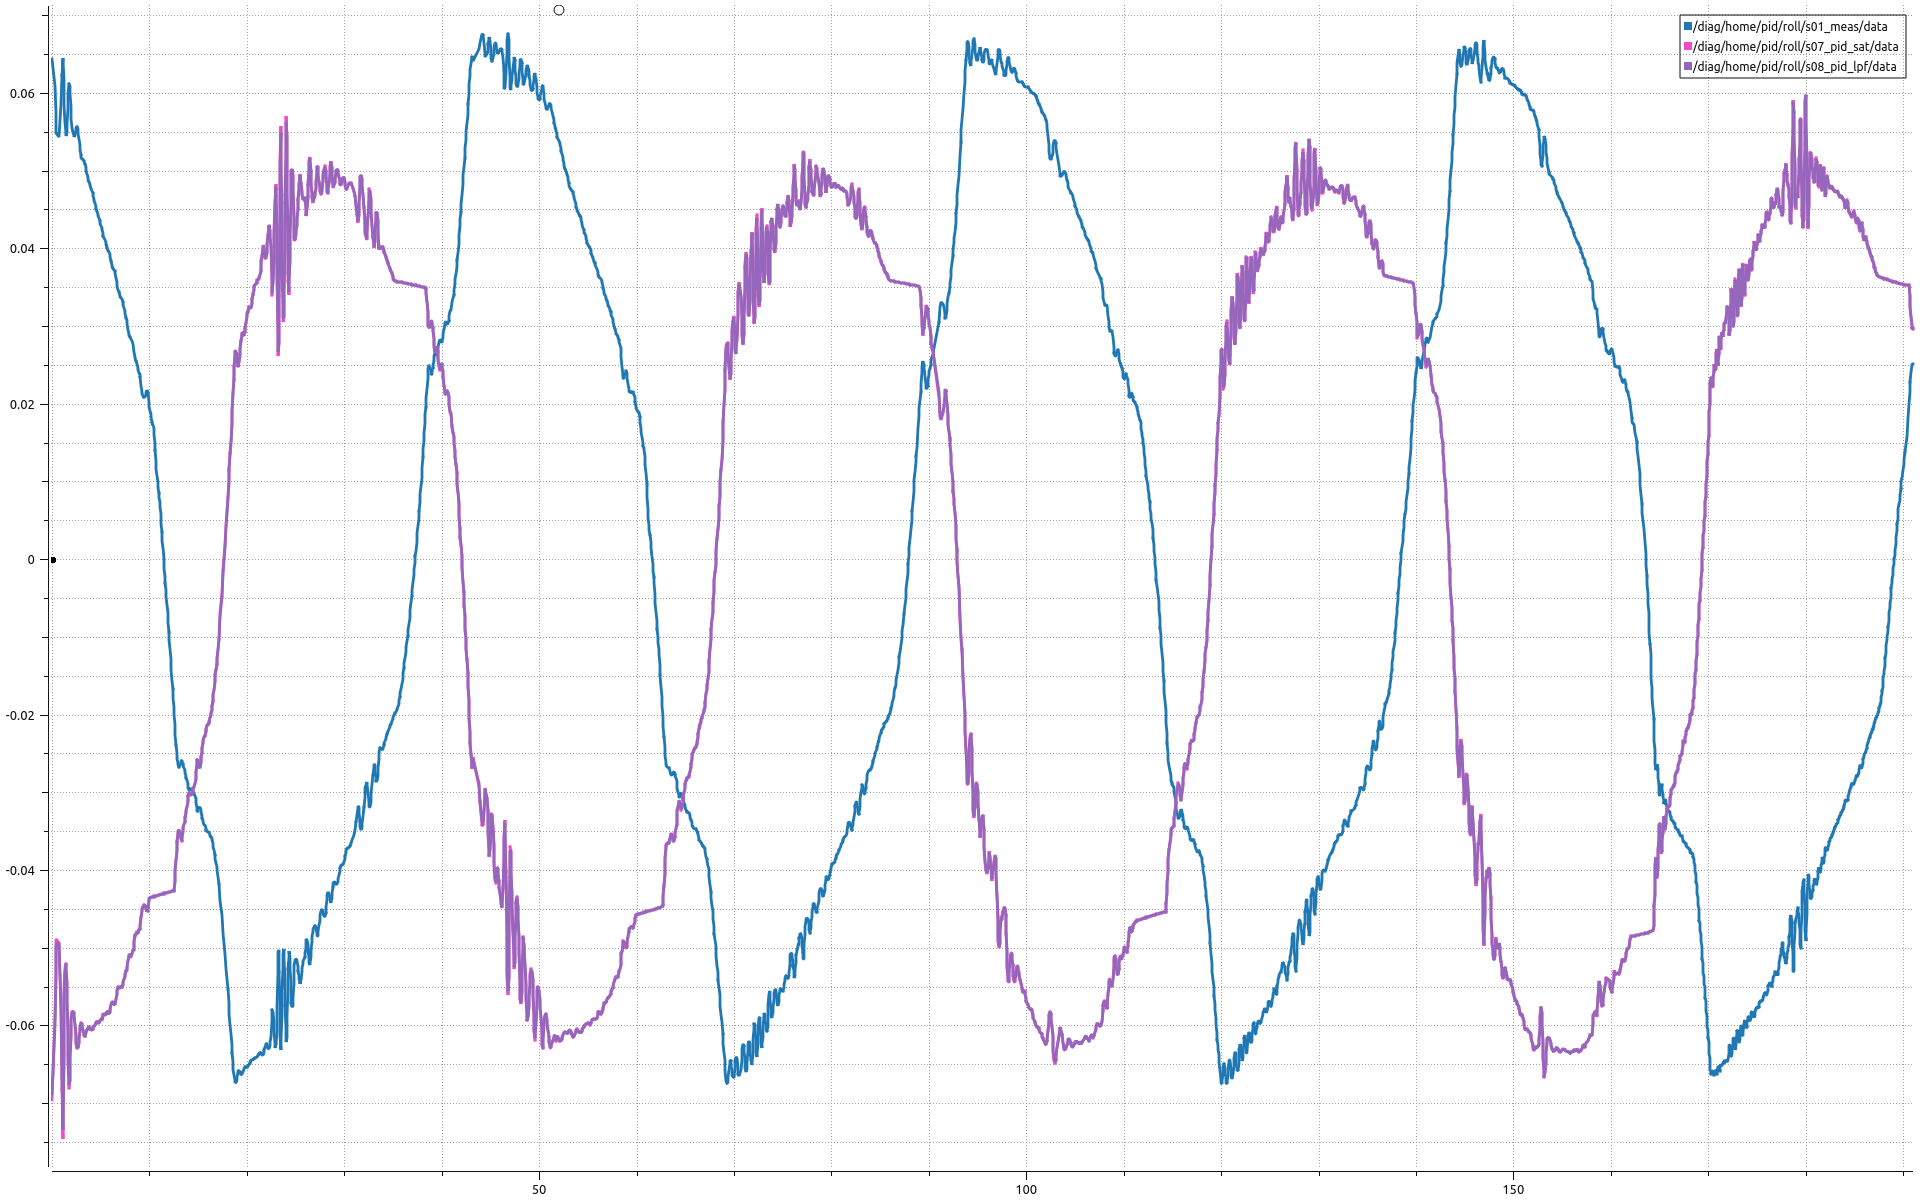
\includegraphics[width=\textwidth]{results/home_pid_roll_controller_meas_sat_lpf.png}
        \caption{Xử lý tín hiệu và đầu ra (Roll)}
        \label{fig:home_pid_roll_meas}
    \end{subfigure}
    \hfill
    \begin{subfigure}[b]{0.48\textwidth}
        \centering
        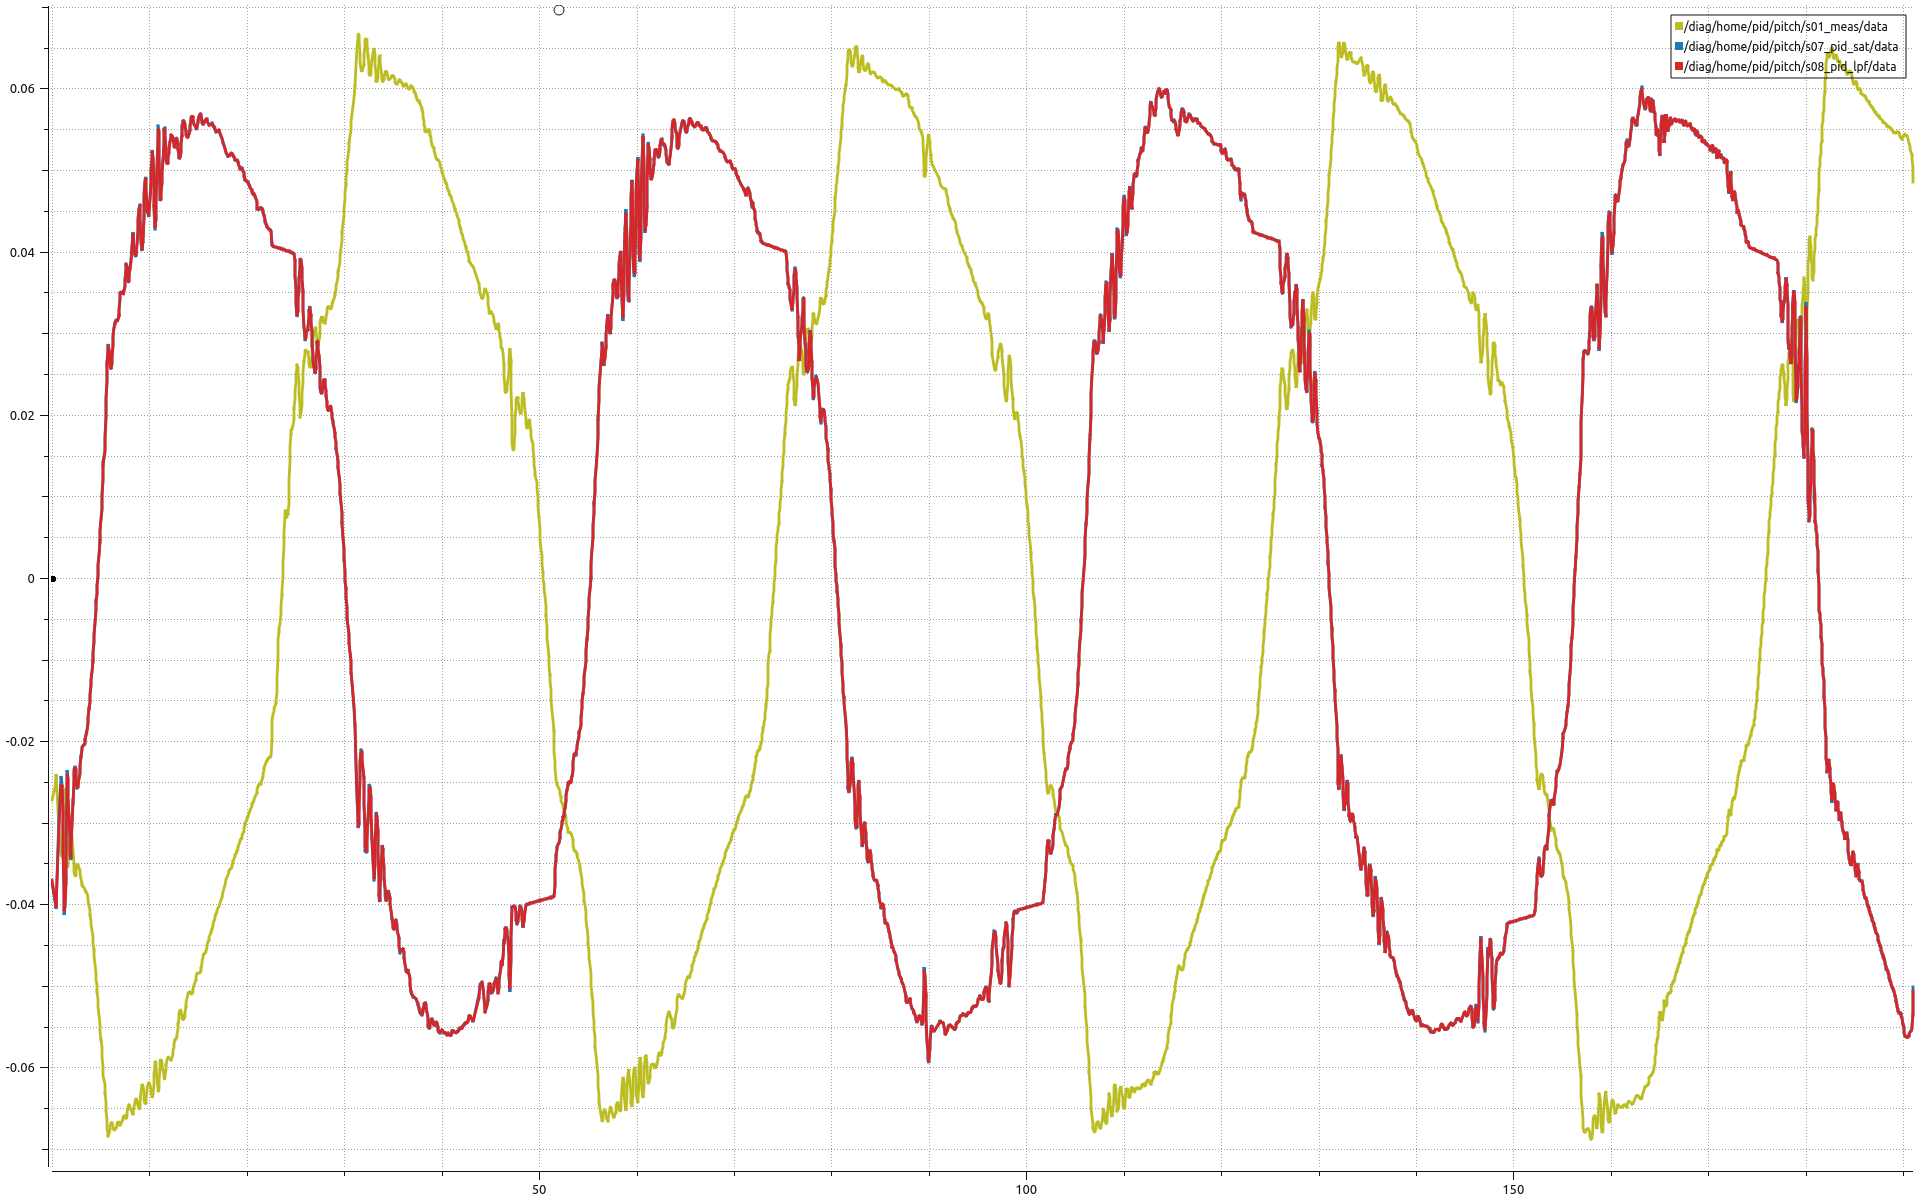
\includegraphics[width=\textwidth]{results/home_pid_pitch_controller_meas_sat_lpf.png}
        \caption{Xử lý tín hiệu và đầu ra (Pitch)}
        \label{fig:home_pid_pitch_meas}
    \end{subfigure}
    \caption{Phân tích tín hiệu đo lường và đầu ra chế độ HOME}
\end{figure}

Hình \ref{fig:home_pid_roll_pid} và Hình \ref{fig:home_pid_pitch_pid} phân rã ba thành phần P, I, D của bộ điều khiển (Giai đoạn 3). Thành phần tỷ lệ (P) đáp ứng ngay lập tức với sai lệch góc nghiêng, trong khi thành phần vi phân (D) phản ứng với tốc độ thay đổi góc để dập tắt dao động. Thành phần tích phân (I) tích lũy để triệt tiêu sai số xác lập nhưng được kiểm soát chặt chẽ bởi cơ chế chống windup và rò rỉ hàm mũ, không bị tăng vọt vượt ngưỡng an toàn trong suốt quá trình phục hồi tư thế.

\begin{figure}[H]
    \centering
    \begin{subfigure}[b]{0.48\textwidth}
        \centering
        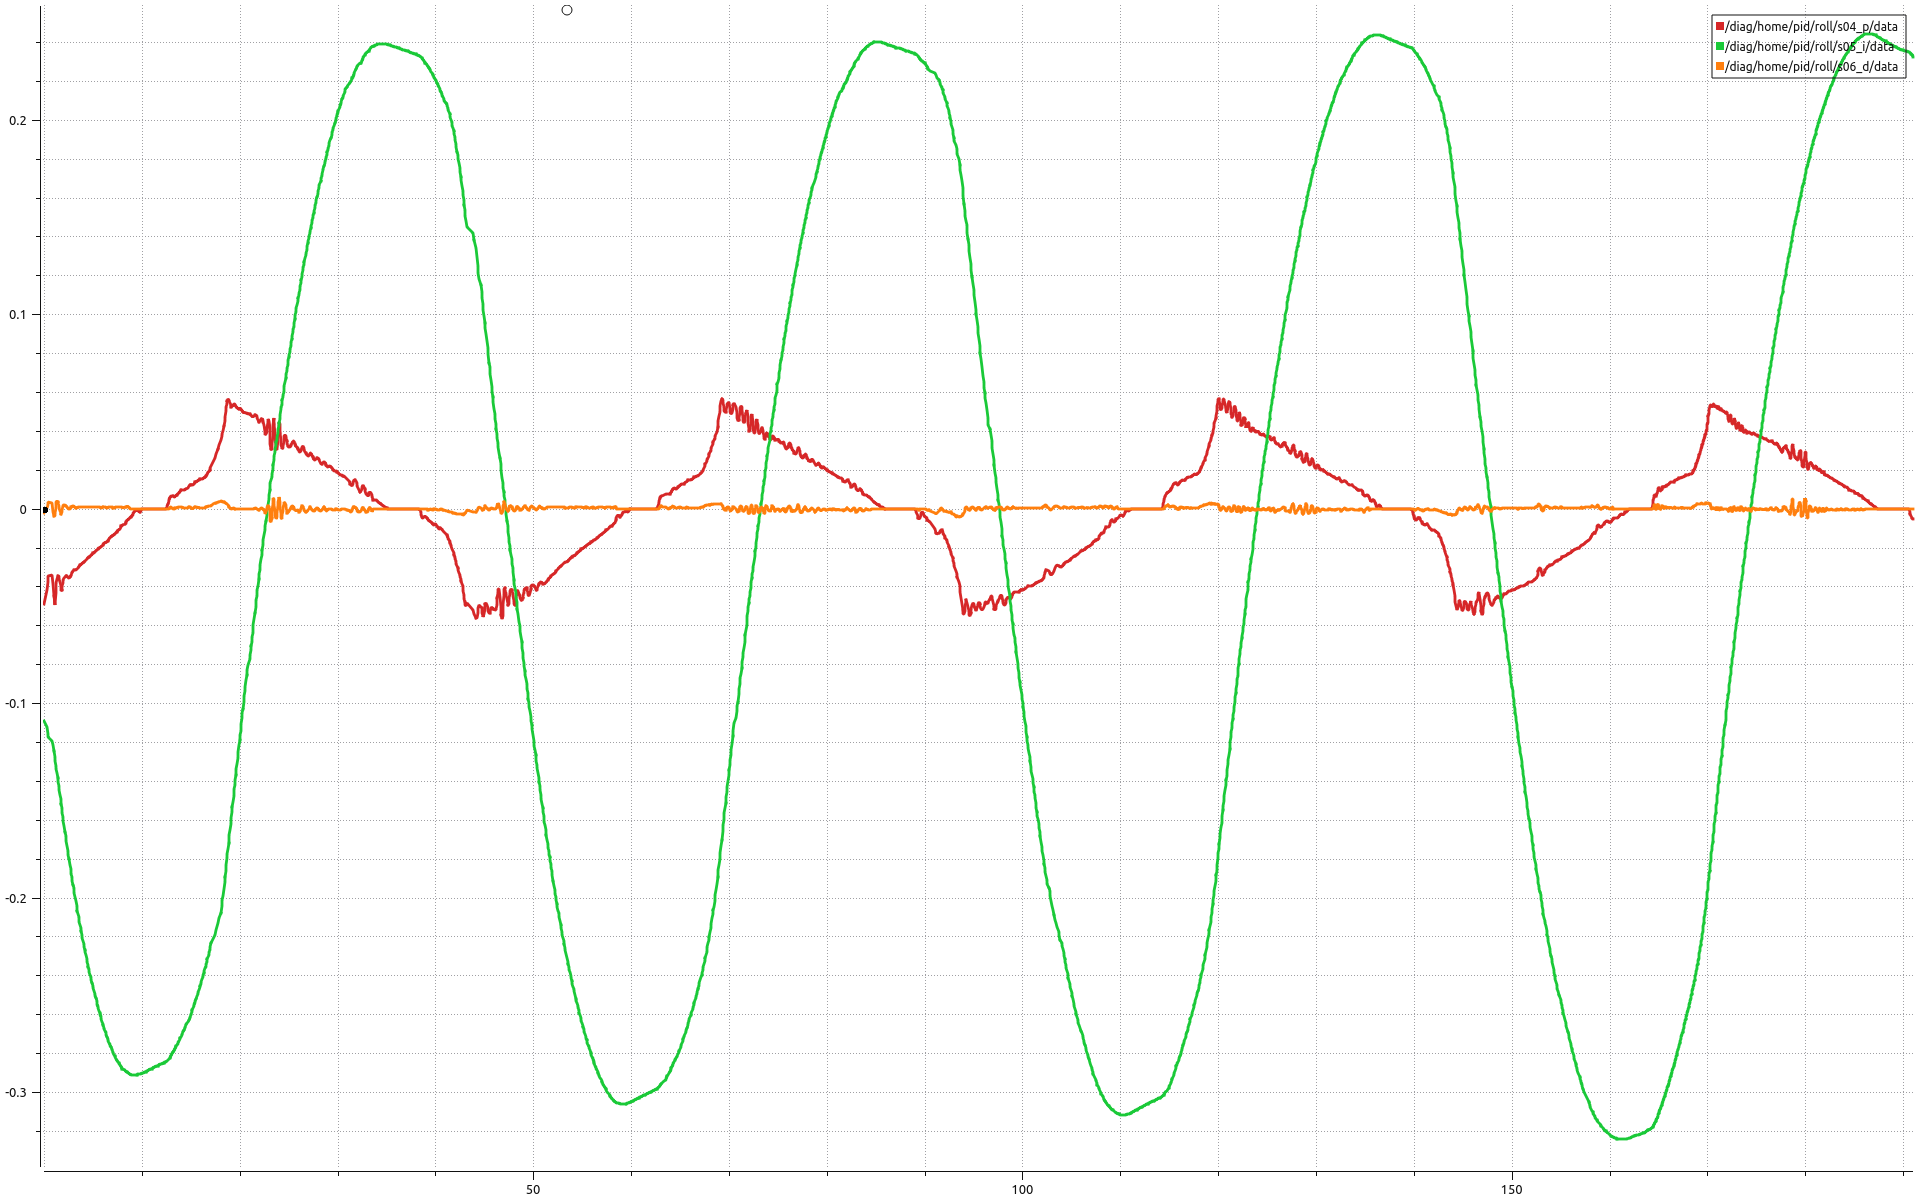
\includegraphics[width=\textwidth]{results/home_pid_roll_controller_p_i_d.png}
        \caption{Thành phần P, I, D (Roll)}
        \label{fig:home_pid_roll_pid}
    \end{subfigure}
    \hfill
    \begin{subfigure}[b]{0.48\textwidth}
        \centering
        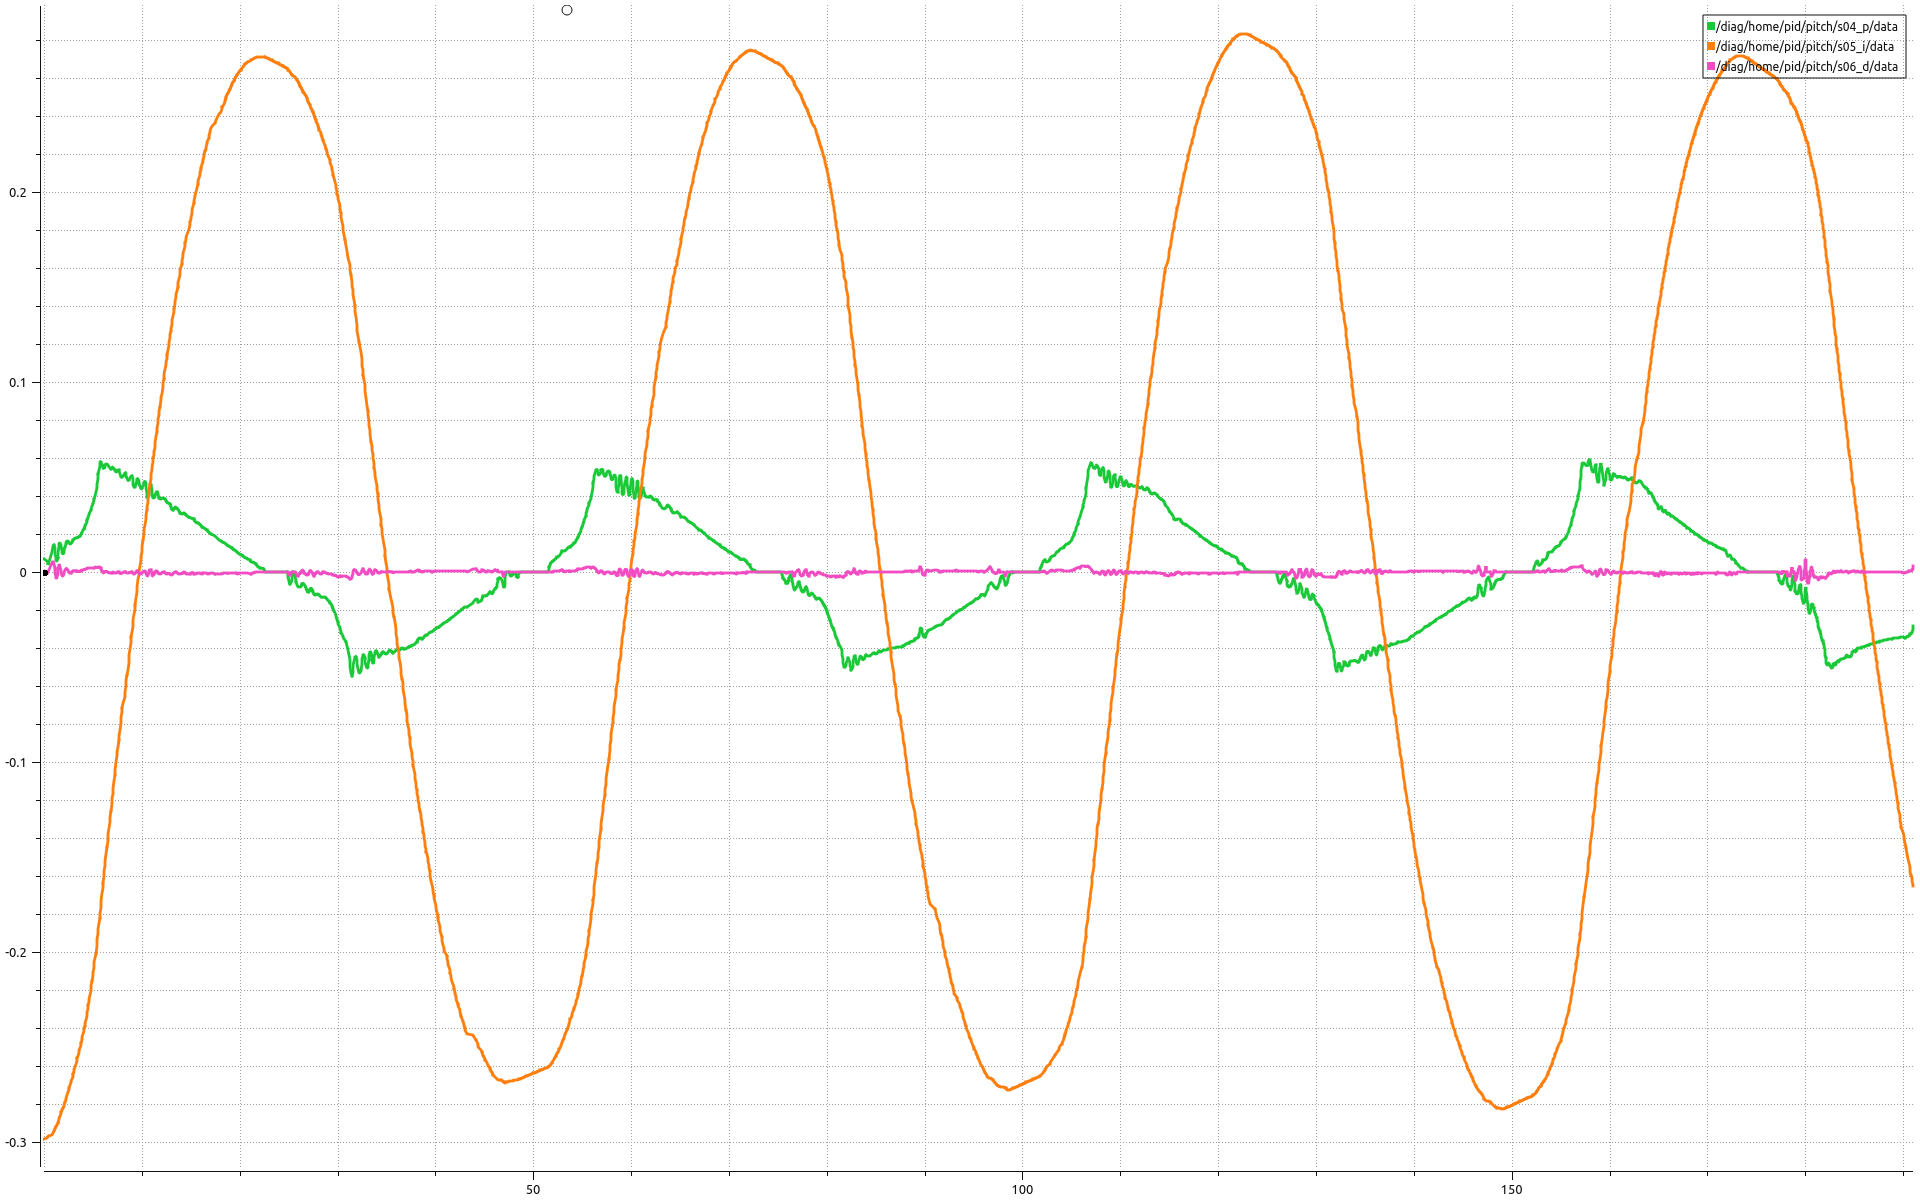
\includegraphics[width=\textwidth]{results/home_pid_pitch_controller_p_i_d.png}
        \caption{Thành phần P, I, D (Pitch)}
        \label{fig:home_pid_pitch_pid}
    \end{subfigure}
    \caption{Phân rã thành phần động học PID chế độ HOME}
\end{figure}

\subsection{Ổn định động trong dáng đi Trot (chế độ GAIT)}

Hình~\ref{fig_pid_gait} phân tích bài toán ổn định tư thế trong chế độ GAIT (dáng đi Trot), nơi bộ điều khiển đối mặt với thách thức phức tạp hơn nhiều do va đập chu kỳ từ các bước chân sinh ra nhiễu động học. Ý nghĩa cốt lõi của đồ thị này là chứng minh sự vượt trội của cấu trúc PID: thay vì bị "đánh lừa" và phản ứng thái quá với các rung lắc tự nhiên của dáng đi (có những đỉnh nhiễu lên tới $\sim 0{,}15$ rad), bộ điều khiển đã duy trì thành công biên độ sai lệch định hướng xoay quanh mức an toàn $0{,}08$ rad. Năng lực này giải quyết triệt để bài toán trôi dạt tư thế (attitude drift), đảm bảo thân robot vận động phẳng, liên tục và không bị lật nhào khi di chuyển quãng đường dài.

\begin{figure}[H]
    \centering
    
\includegraphics[width=0.85\textwidth]{results/pid_error_gait.png}
    \caption{Đáp ứng sai lệch bộ điều khiển trong chế độ động GAIT (dáng đi Trot)}
    \label{fig_pid_gait}
\end{figure}

\subsubsection*{Phân tích tín hiệu nội bộ chuỗi xử lý PID (Chế độ GAIT)}

Trong chế độ di chuyển (GAIT), bộ điều khiển phải đối mặt với các nhiễu loạn có tính chu kỳ sinh ra từ bước chân chạm đất. Chuỗi xử lý được bổ sung các cơ chế xử lý đặc thù để duy trì ổn định.

Hình \ref{fig:trot_pid_meas} minh họa hoạt động của cơ chế đường cơ sở trung bình trượt (Moving Average Baseline). Thuật toán này sinh ra để giải quyết bài toán "nhận diện nhầm" (false positive) rất phổ biến trong điều khiển động học chân. Khi robot bước đi, thân máy tất yếu sẽ dao động theo nhịp. Nếu PID lấy giá trị tuyệt đối $0$ làm mốc, nó sẽ liên tục xuất lệnh "chống lại" bước đi của chính con robot. Việc sử dụng đường tham chiếu động (đường baseline mượt) giúp hệ thống thông minh hơn: nó bỏ qua sự lắc lư tự nhiên và chỉ xuất lệnh bù khi thân robot thực sự mất trọng tâm do tác động của ngoại lực hay địa hình dốc.

\begin{figure}[H]
    \centering
    \begin{subfigure}[b]{0.48\textwidth}
        \centering
        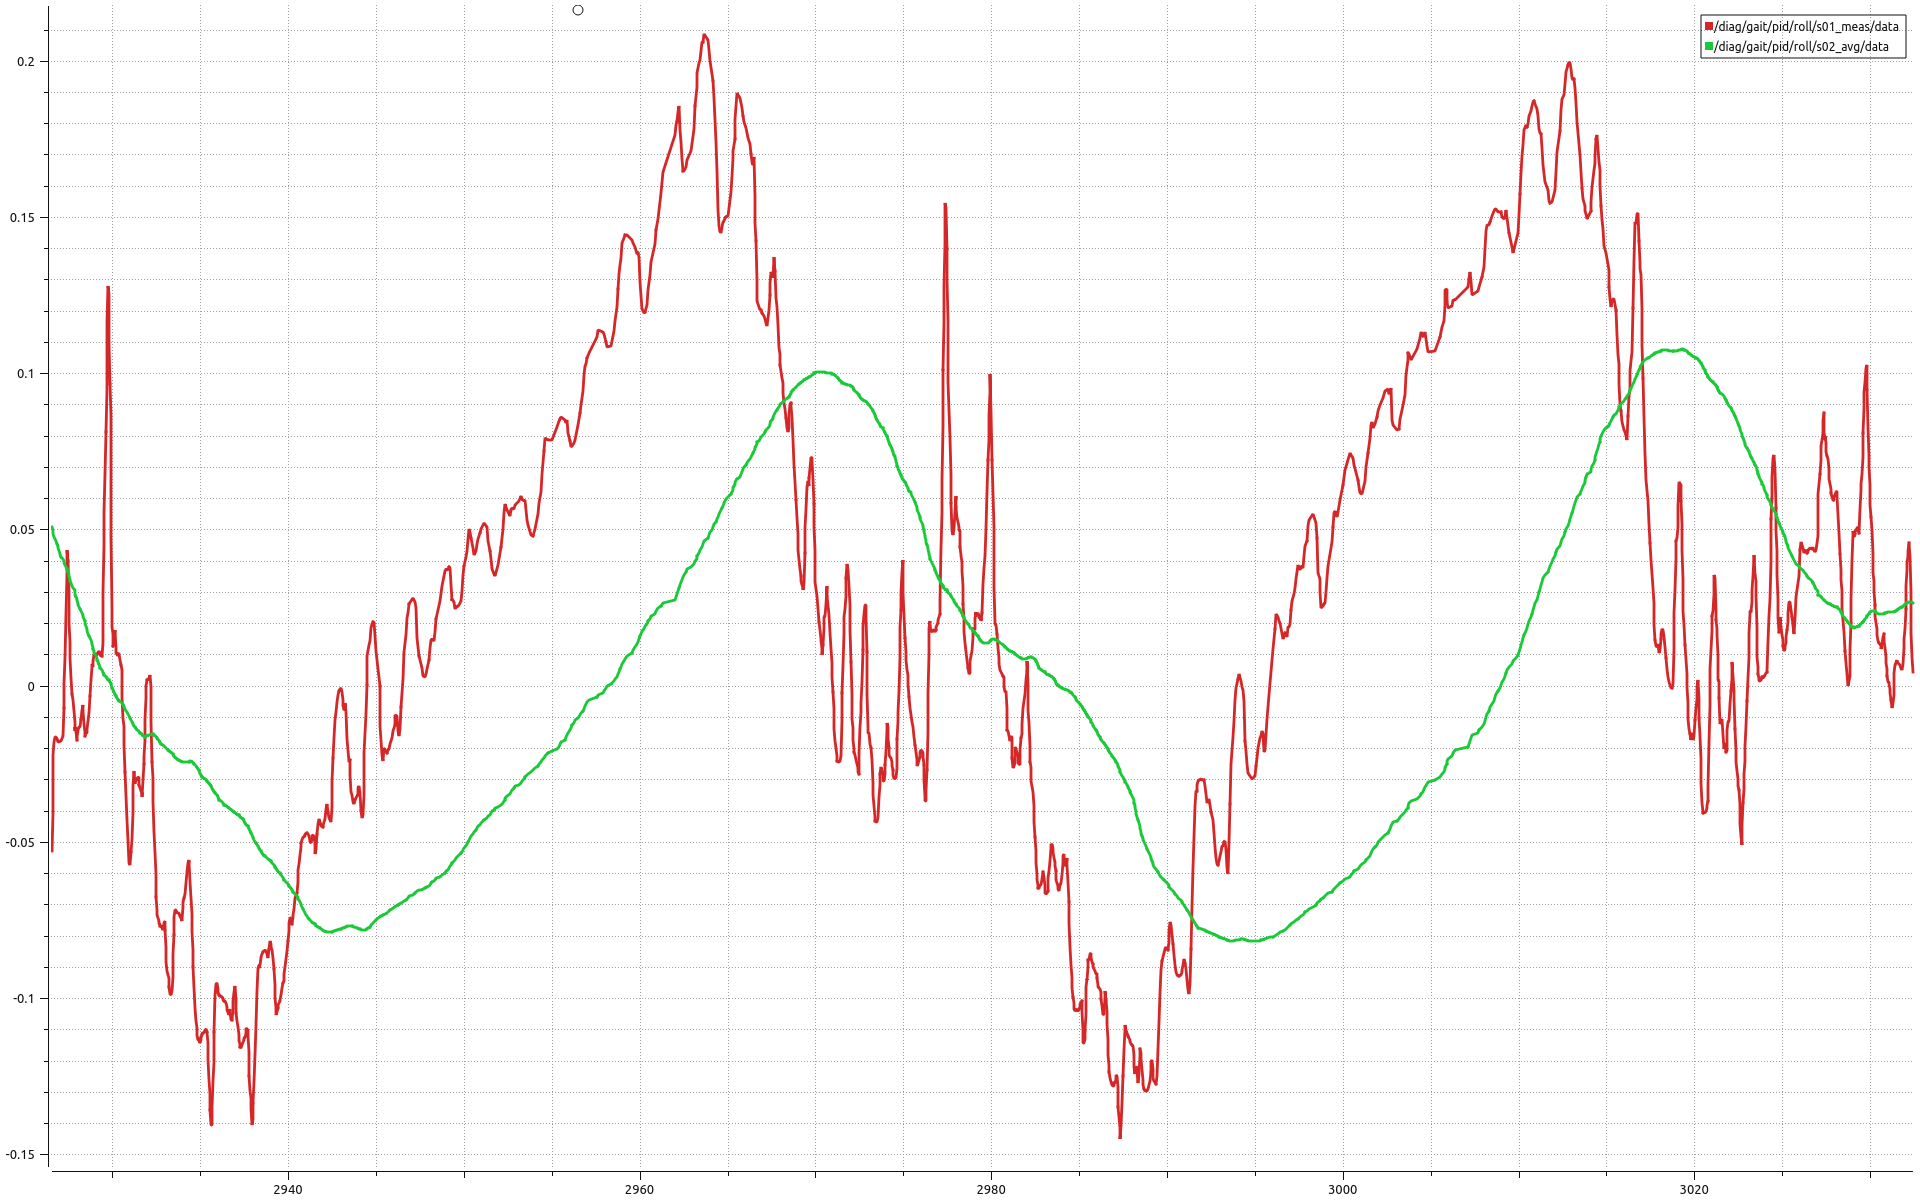
\includegraphics[width=\textwidth]{results/trot_pid_roll_controller_meas_avg_zoom.png}
        \caption{Cơ chế đường cơ sở trung bình (Roll)}
    \end{subfigure}
    \hfill
    \begin{subfigure}[b]{0.48\textwidth}
        \centering
        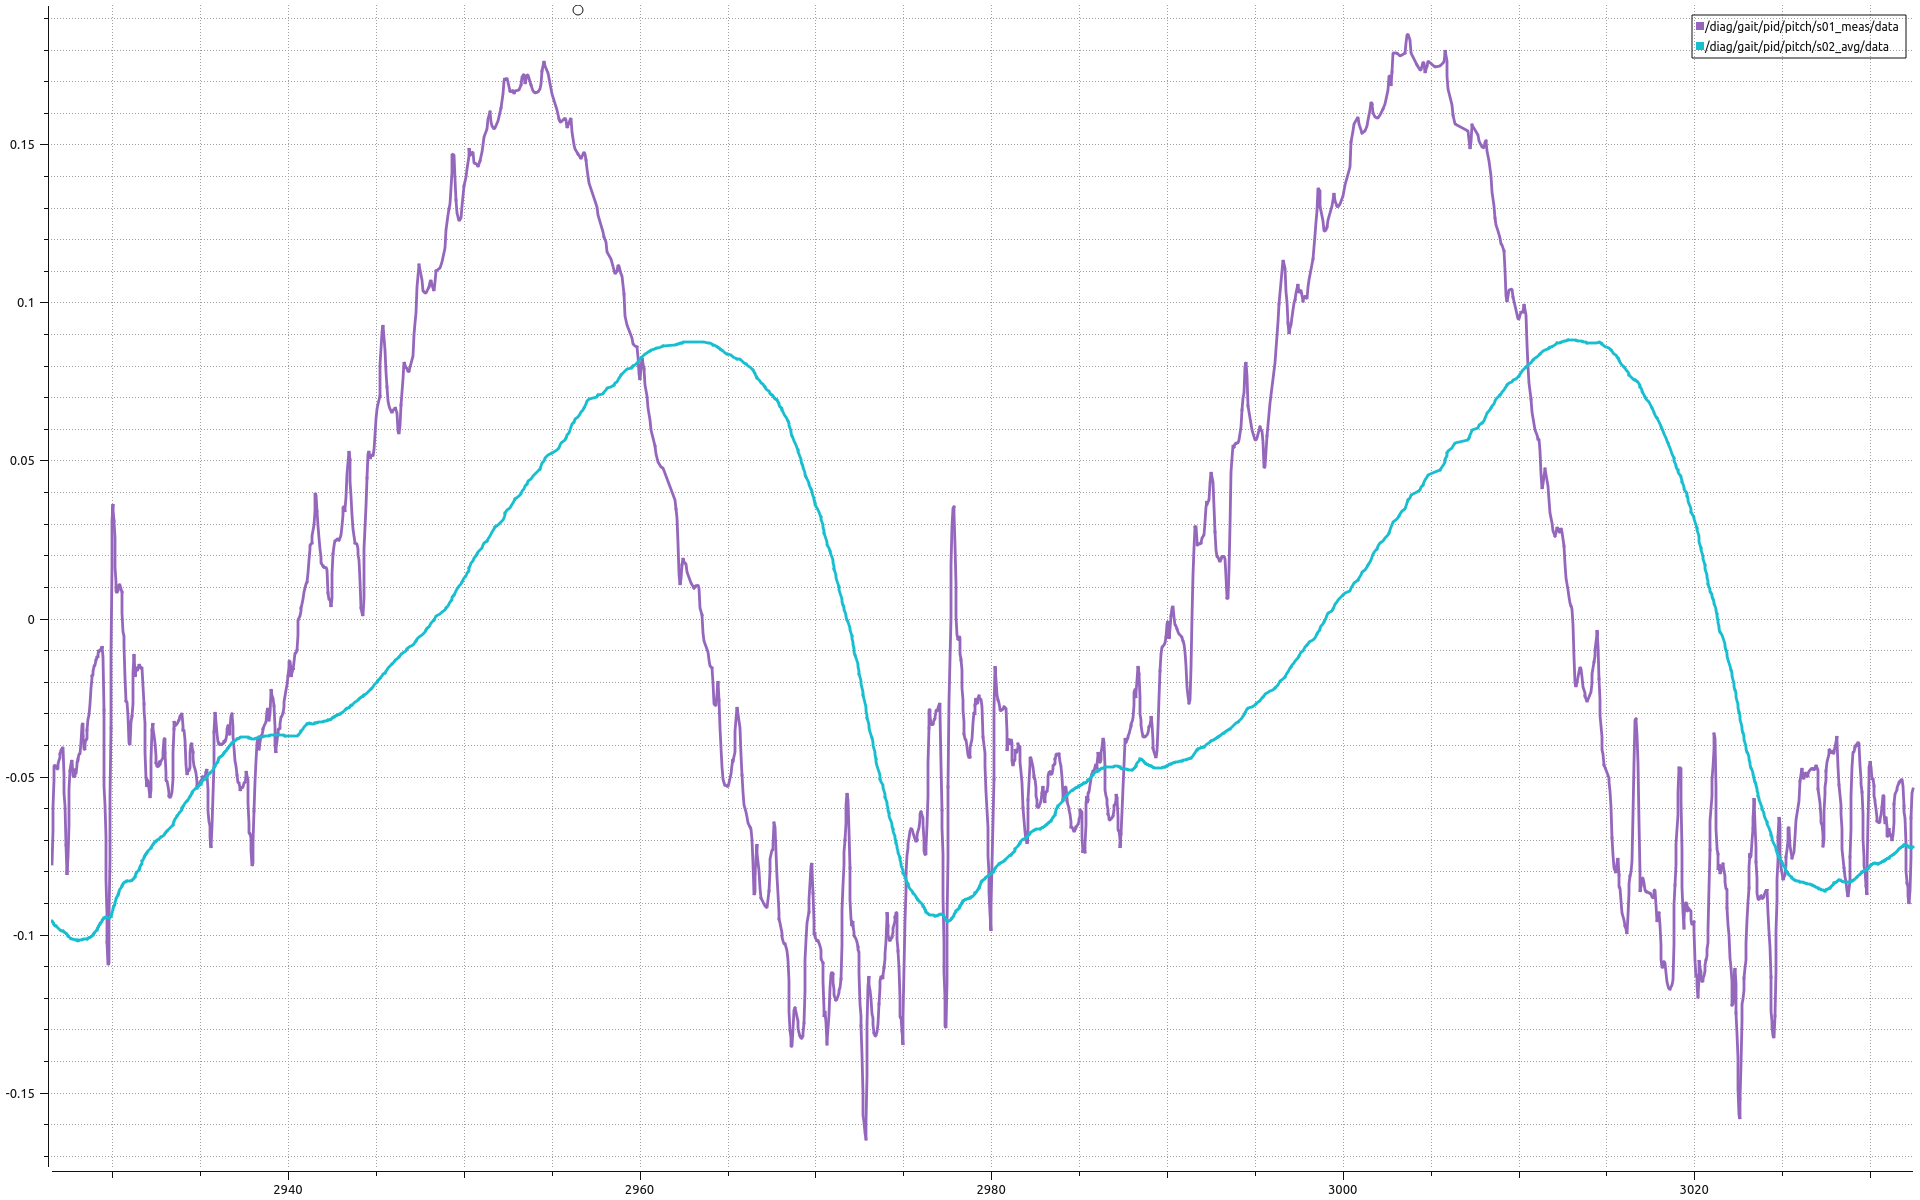
\includegraphics[width=\textwidth]{results/trot_pid_pitch_controller_meas_avg_zoom.png}
        \caption{Cơ chế đường cơ sở trung bình (Pitch)}
    \end{subfigure}
    \caption{Phân tích xử lý tín hiệu đầu vào chế độ GAIT (phóng to)}
    \label{fig:trot_pid_meas}
\end{figure}

Sự phân rã các thành phần PID trong Hình \ref{fig:trot_pid_pid} đặc biệt nhấn mạnh vào vai trò định hình của khâu Tích phân (I). Trong hệ thống di chuyển tuần hoàn như Trot, thân robot lắc qua lắc lại liên tục qua trục cân bằng. Nếu áp dụng PID truyền thống, khâu I sẽ tích lũy lỗi theo thời gian và gây ra hiện tượng quá điều chỉnh (overshoot) nghiêm trọng khi robot chuyển trụ giữa các chân. Việc thiết kế cơ chế reset tích phân tại giao điểm 0 (Zero Crossing Integral Reset) giải quyết dứt điểm rủi ro này, ép bộ điều khiển phải "quên" đi các sai lệch cũ ngay khi hệ thống vừa vượt chéo qua trạng thái cân bằng.

\begin{figure}[H]
    \centering
    \begin{subfigure}[b]{0.48\textwidth}
        \centering
        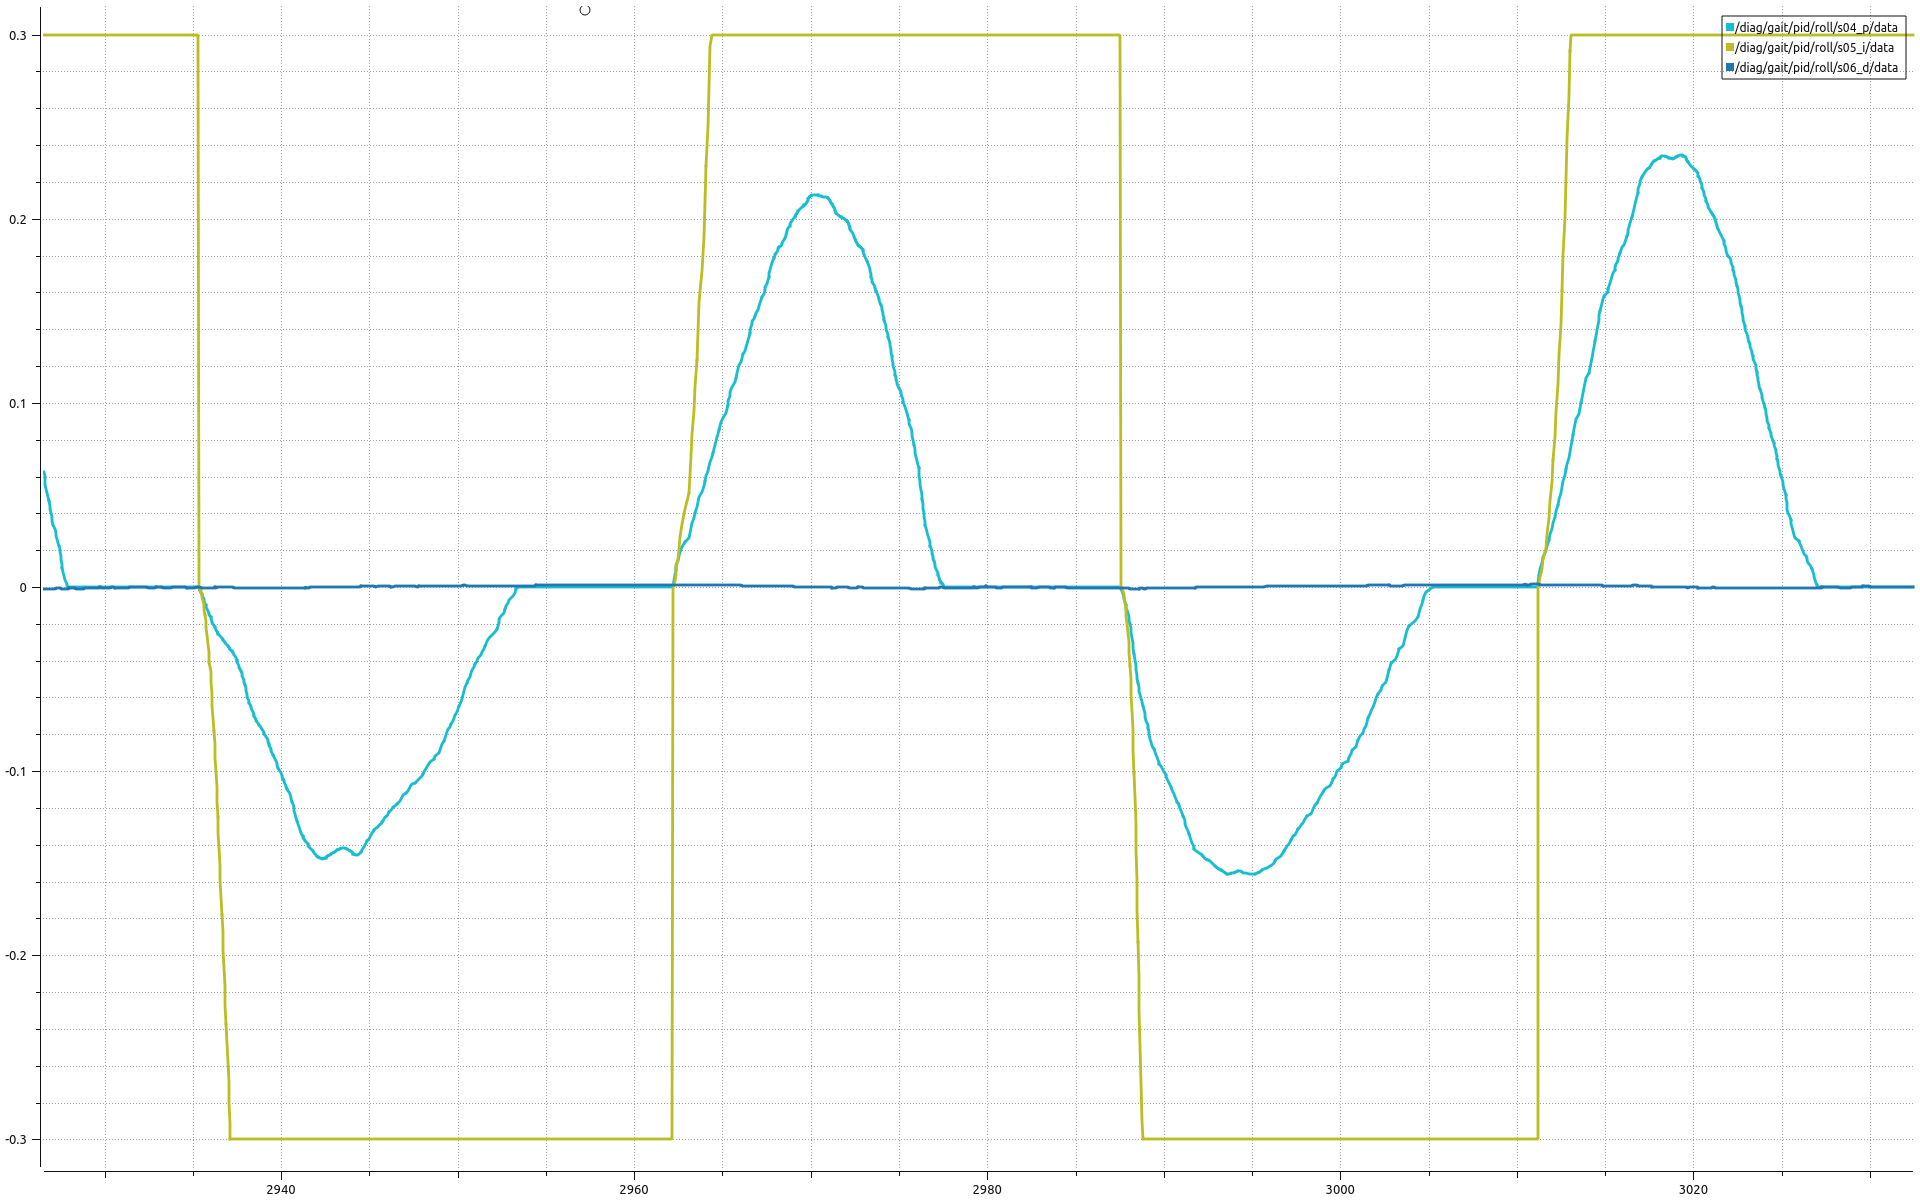
\includegraphics[width=\textwidth]{results/trot_pid_roll_controller_p_i_d_zoom.png}
        \caption{Thành phần P, I, D (Roll)}
    \end{subfigure}
    \hfill
    \begin{subfigure}[b]{0.48\textwidth}
        \centering
        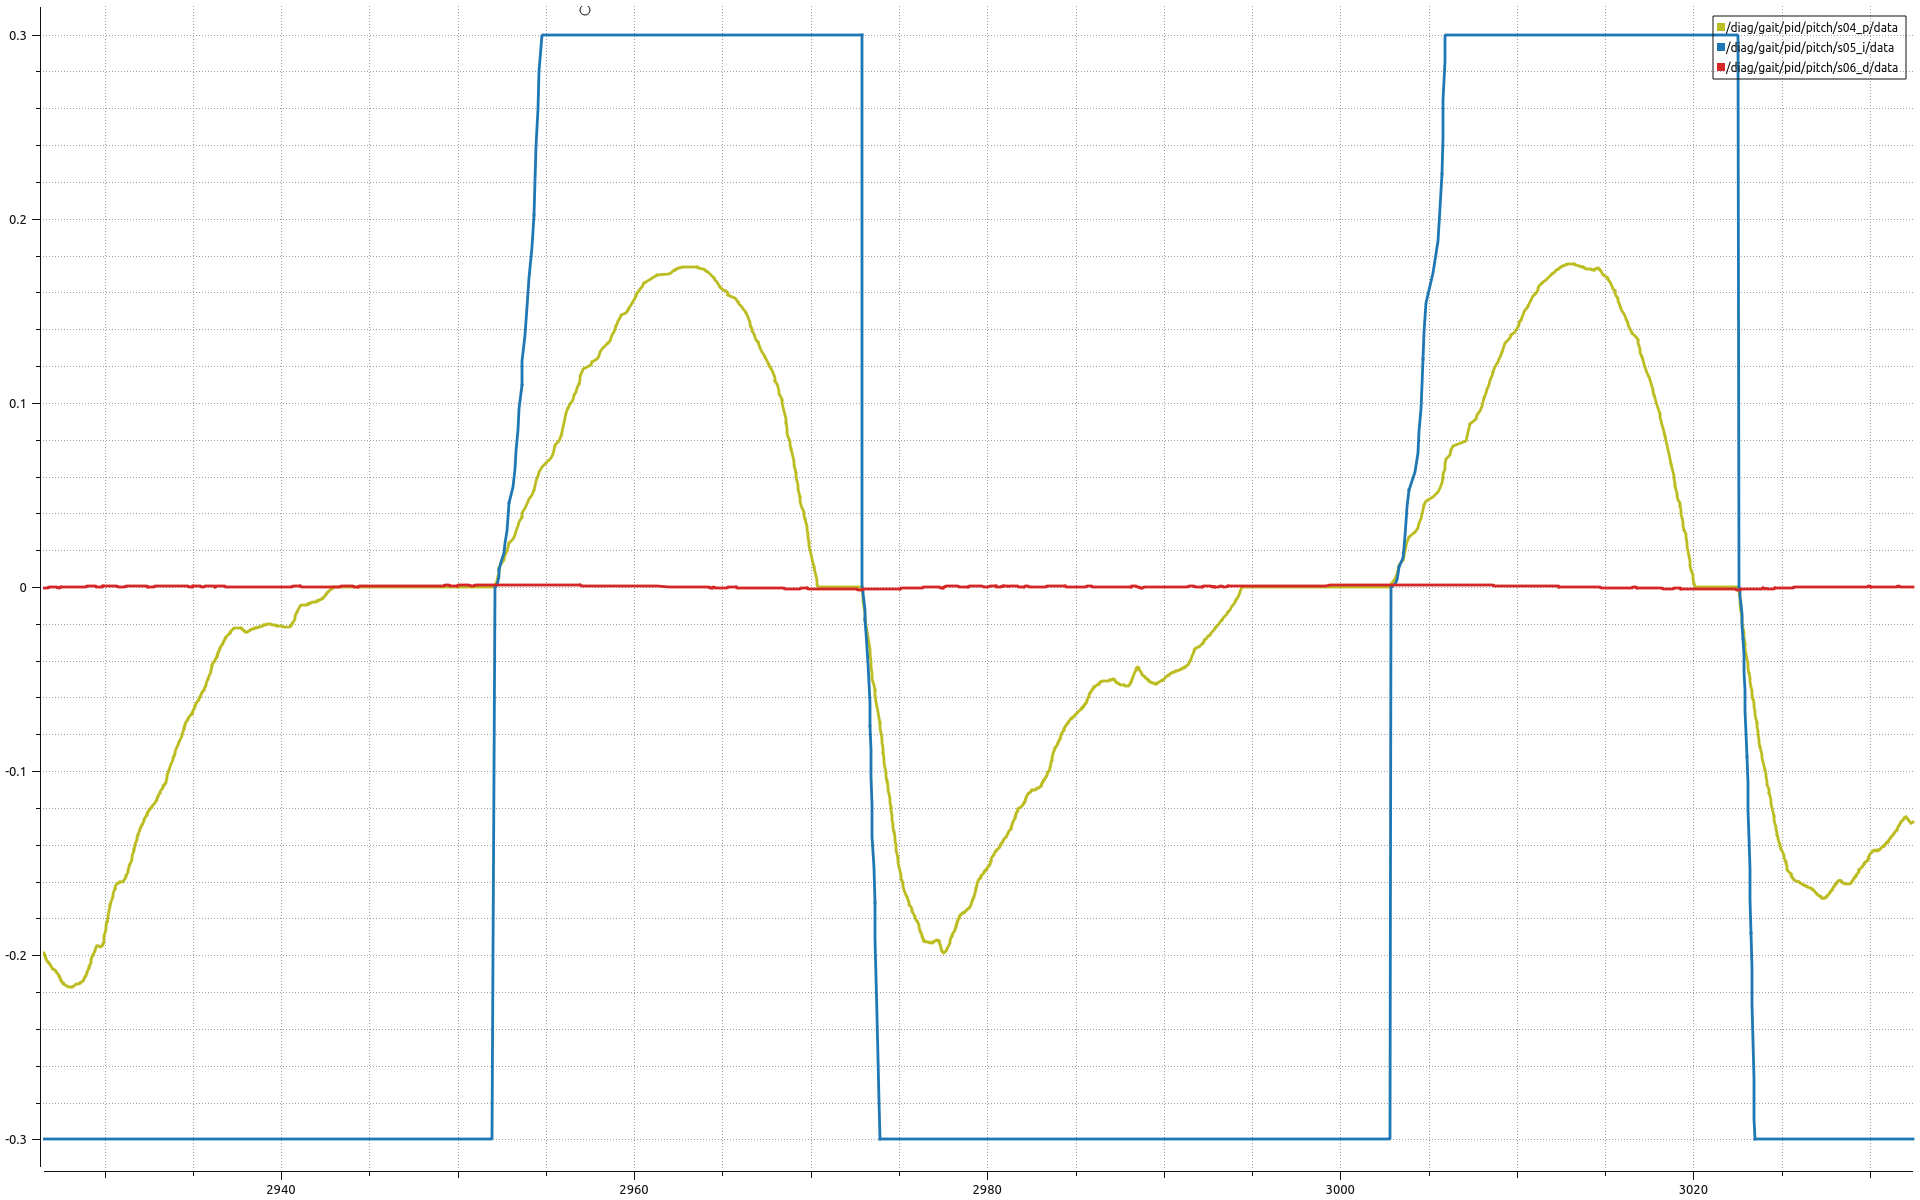
\includegraphics[width=\textwidth]{results/trot_pid_pitch_controller_p_i_d_zoom.png}
        \caption{Thành phần P, I, D (Pitch)}
    \end{subfigure}
    \caption{Phân rã thành phần động học PID chế độ GAIT (phóng to)}
    \label{fig:trot_pid_pid}
\end{figure}

Cuối cùng, Hình \ref{fig:trot_pid_sat_lpf} minh họa lý do phải phân tách bộ tham số LPF độc lập cho từng chế độ. Trong chế độ GAIT, nếu lệnh cân bằng được xuất ra quá gắt, nó sẽ phá vỡ động học của các chân đang đảm nhận nhiệm vụ chống đỡ thân (stance phase), làm chân bị trượt hoặc bước hụt. Vì vậy, việc siết chặt bão hòa ($u_{max} = 0{,}30$ rad) và tăng cường cường độ lọc LPF ($\alpha = 0{,}97$) mang ý nghĩa nhượng bộ chiến lược: hệ thống ưu tiên bảo toàn quỹ đạo sải bước nguyên vẹn, chỉ sử dụng một lực bù biên độ rất nhỏ và mềm mại để từ từ điều hướng trọng tâm, từ đó giải quyết bài toán xung đột cơ học giữa "nhiệm vụ bước đi" và "nhiệm vụ cân bằng".

\begin{figure}[H]
    \centering
    \begin{subfigure}[b]{0.48\textwidth}
        \centering
        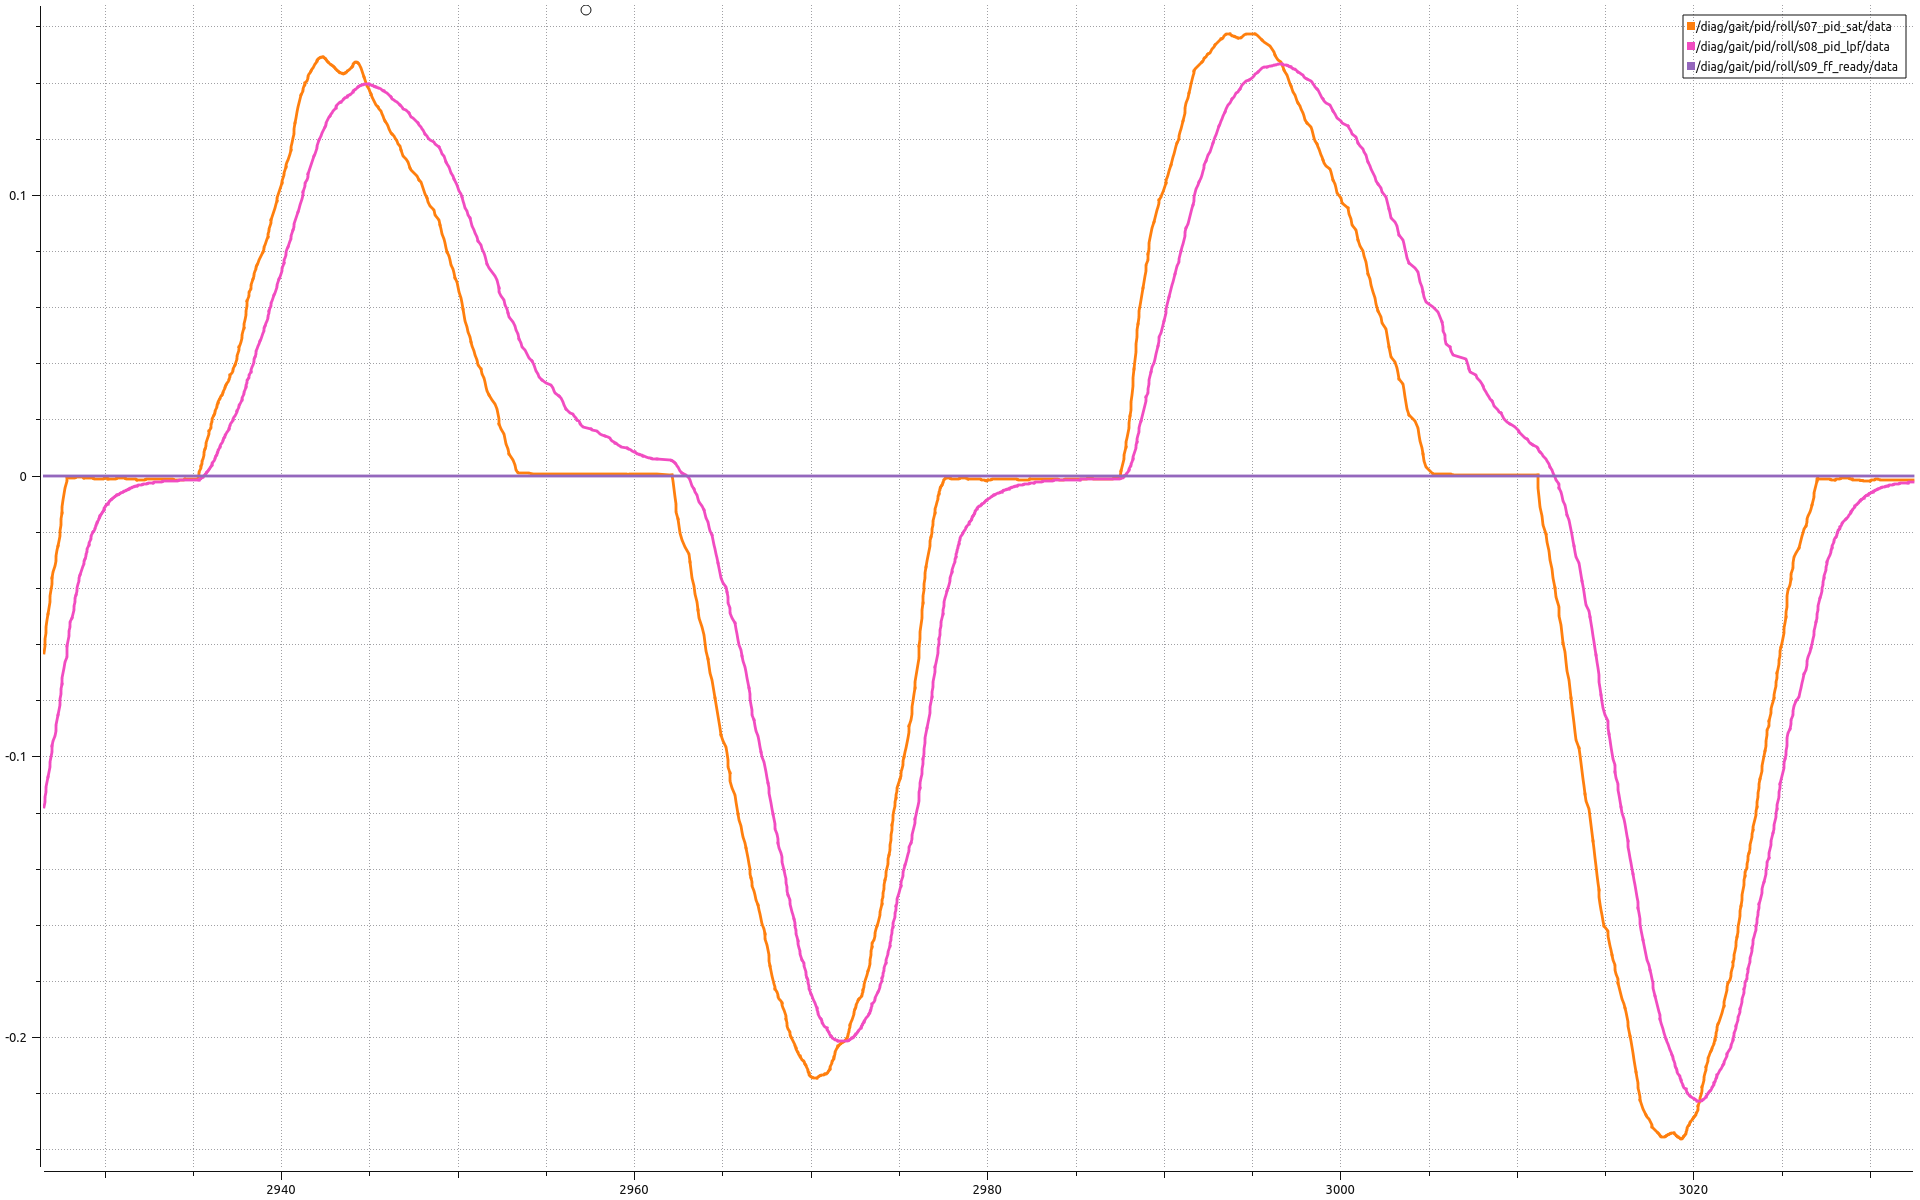
\includegraphics[width=\textwidth]{results/trot_pid_roll_controller_sat_lpf_ff_zoom.png}
        \caption{Xử lý tín hiệu đầu ra (Roll)}
    \end{subfigure}
    \hfill
    \begin{subfigure}[b]{0.48\textwidth}
        \centering
        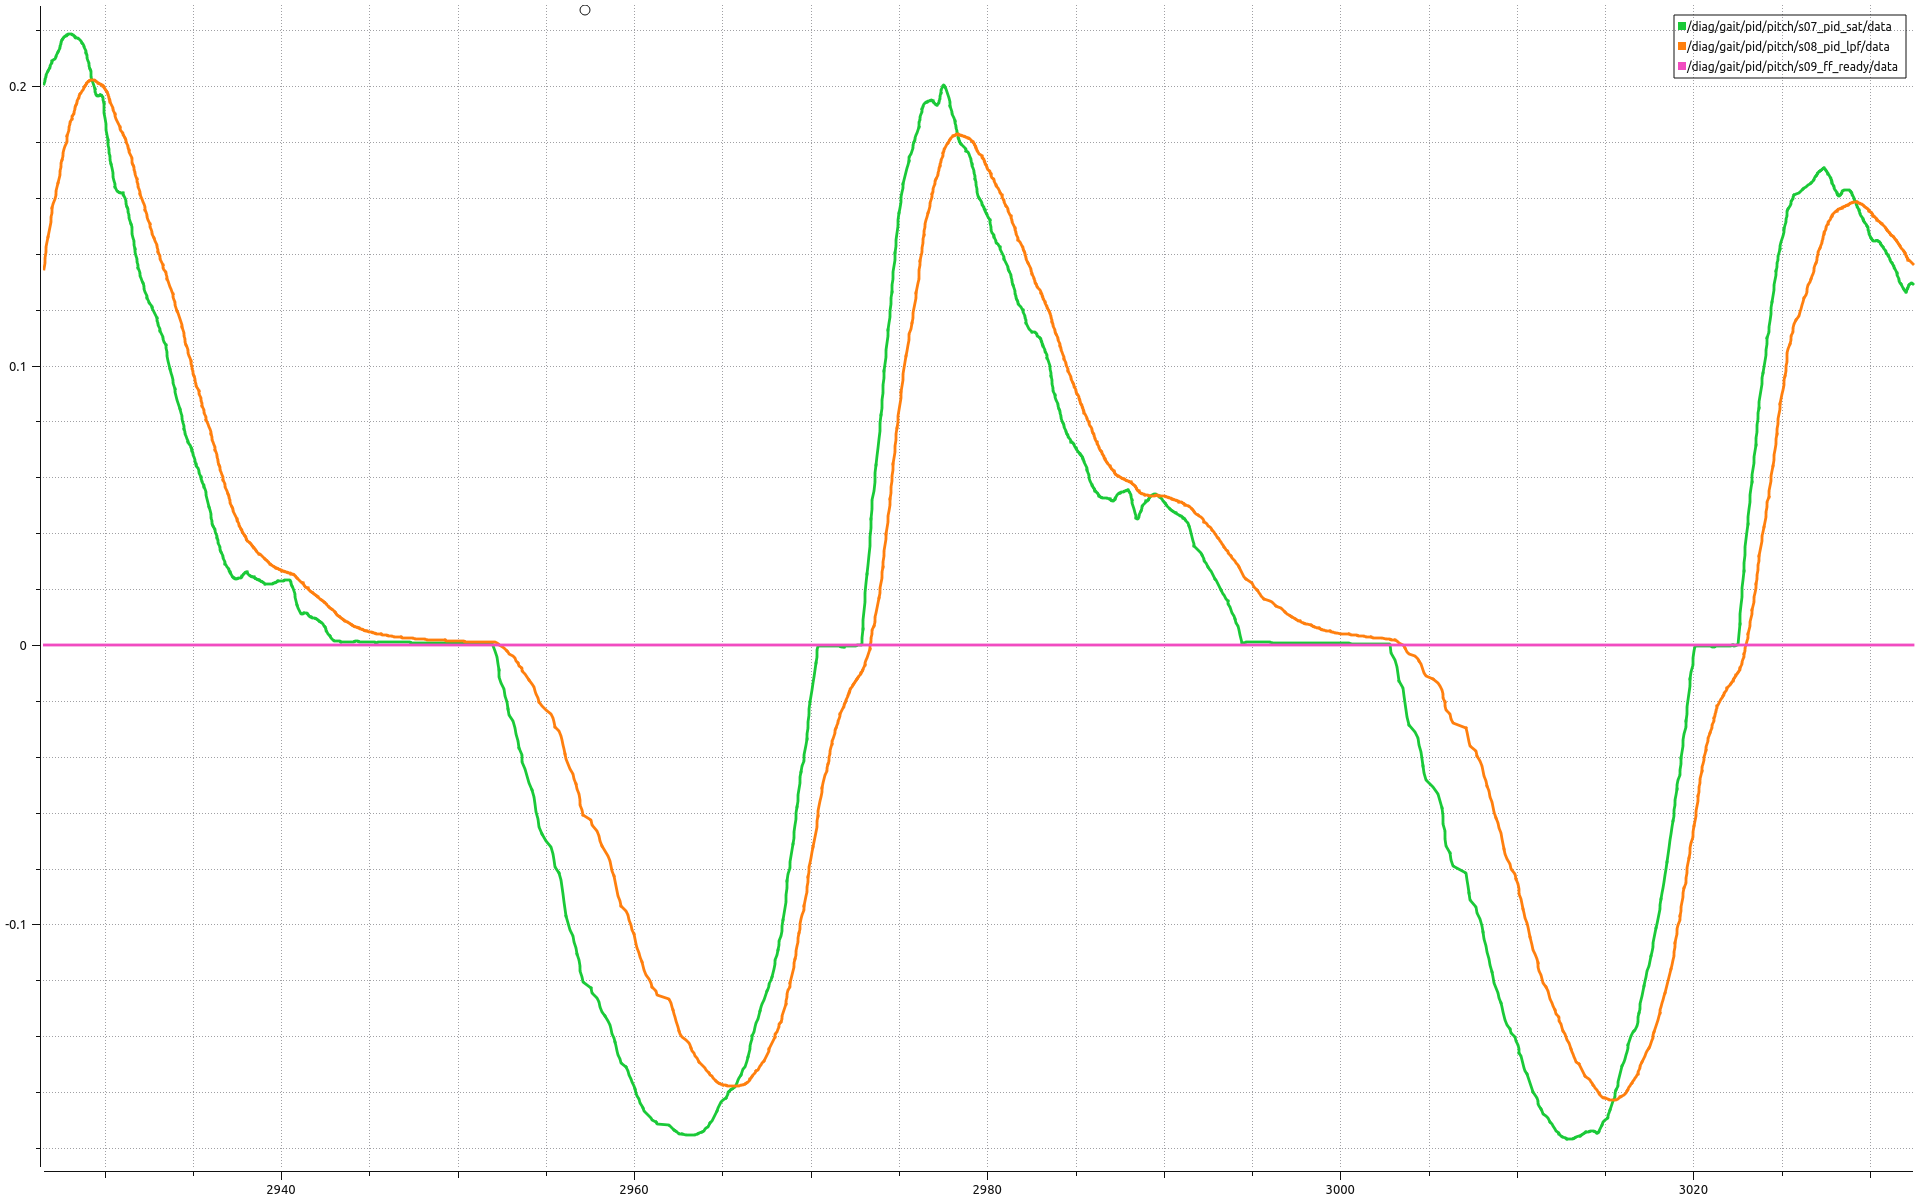
\includegraphics[width=\textwidth]{results/trot_pid_pitch_controller_sat_lpf_ff_zoom.png}
        \caption{Xử lý tín hiệu đầu ra (Pitch)}
    \end{subfigure}
    \caption{Phân tích bão hòa và lọc đầu ra chế độ GAIT (phóng to)}
    \label{fig:trot_pid_sat_lpf}
\end{figure}


%% ====================================================================
%%  PHẦN THỰC NGHIỆM PHẦN CỨNG
%% ====================================================================

\section{Thực nghiệm trên phần cứng thực}

\subsection{Giới thiệu}

Sau khi xác minh tính đúng đắn của các thuật toán thông qua mô phỏng ROS~2/Gazebo, toàn bộ hệ thống phần mềm được triển khai trên phần cứng thực nhằm đánh giá khả năng vận hành của robot trong điều kiện thực tế. Mục tiêu của giai đoạn thực nghiệm bao gồm việc kiểm chứng khả năng khởi tạo tư thế đứng (homing) từ vị trí ngẫu nhiên, đánh giá hiệu quả của dáng đi Trot trên mặt phẳng nằm ngang, kiểm tra tính ổn định của cơ chế tắt an toàn ba pha, và cuối cùng là so sánh đối chiếu kết quả thực nghiệm với các dữ liệu đã thu được từ môi trường mô phỏng.

\subsection{Mô hình robot thực tế}

Mô hình robot bốn chân đã được lắp ráp hoàn chỉnh với các thành phần chính: khung thân in 3D (PLA), 12 động cơ bus servo ST3215, máy tính nhúng Jetson Nano B01, cảm biến IMU BNO055, hai mạch Bus Servo Adapter (A), mạch giảm áp XL4015 và nguồn xung tổ ong 12~V -- 40~A. Tổng khối lượng robot (không bao gồm nguồn và dây cáp) vào khoảng 3{,}5~kg.

\begin{table}[H]
\centering
\caption{Thông số hình học robot thực tế}
\label{tab:hw_robot_params}
\renewcommand{\arraystretch}{1.3}
\begin{tabular}{|l|c|c|l|}
\hline
\textbf{Tham số} & \textbf{Ký hiệu} & \textbf{Giá trị} & \textbf{Đơn vị} \\ \hline
Chiều dài thân robot & $L$ & 209 & mm \\ \hline
Chiều rộng thân robot & $W$ & 191 & mm \\ \hline
Chiều dài khớp coxa & $l_1$ & 26 & mm \\ \hline
Chiều dài xương đùi & $l_2$ & 106 & mm \\ \hline
Chiều dài xương ống chân & $l_3$ & 125 & mm \\ \hline
Tổng khối lượng robot & $m$ & $\sim$3,5 & kg \\ \hline
Số bậc tự do & DOF & 12 & -- \\ \hline
\end{tabular}
\end{table}

\subsection{Kiến trúc khởi động hệ thống phần cứng}

Hệ thống phần cứng thực được khởi động thông qua kịch bản khởi chạy của ROS~2 (launch file), bao gồm ba node chính phối hợp hoạt động. Node thứ nhất là Serial Driver A (\texttt{serial\_driver\_a}), chịu trách nhiệm quản lý 6 servo thuộc chân trước bên trái (LF) và chân sau bên phải (RB) thông qua giao tiếp cổng \texttt{/dev/ttyACM1} với các servo mang ID $[7, 8, 9, 10, 11, 12]$. Node thứ hai là Serial Driver B (\texttt{serial\_driver\_b}), quản lý 6 servo thuộc chân sau bên trái (LB) và chân trước bên phải (RF), thực hiện giao tiếp qua cổng \texttt{/dev/ttyACM0} với nhóm servo ID $[4, 5, 6, 1, 2, 3]$. Node cuối cùng là Leg Controller (\texttt{node\_leg\_controller}), đóng vai trò trung tâm trong việc tính toán giải tích động học nghịch, quy hoạch quỹ đạo di chuyển và gửi các lệnh điều khiển đồng bộ xuống hai driver.

Mỗi serial driver nhận lệnh góc servo (đơn vị độ) từ topic \texttt{/servo\_}\allowbreak\texttt{commands\_}\allowbreak\texttt{a} hoặc \texttt{/servo\_}\allowbreak\texttt{commands\_}\allowbreak\texttt{b}, chuyển đổi sang giá trị tick (0--4095) và gửi qua giao tiếp UART bán song công đến các servo ST3215. Tốc độ truyền (baudrate) được cấu hình ở mức 1~Mbps để đảm bảo đáp ứng thời gian thực.

\subsection{Chuyển đổi góc IK sang góc servo}

Một thách thức quan trọng khi chuyển từ mô phỏng sang phần cứng thực là việc ánh xạ chính xác các góc khớp từ thuật toán IK sang giá trị điều khiển servo. Do cấu trúc lắp đặt cơ khí khác nhau giữa các chân (chiều quay ngược, offset vật lý), mỗi chân cần một hàm chuyển đổi riêng biệt. Các hàm này đã được hiệu chỉnh thực nghiệm (empirically verified) thông qua quá trình calibrate từng servo.

\begin{table}[H]
\centering
\caption{Công thức chuyển đổi IK → Servo cho từng chân}
\label{tab:ik_to_servo}
\renewcommand{\arraystretch}{1.5}
\begin{tabular}{|l|p{0.65\linewidth}|}
\hline
\textbf{Chân} & \textbf{Công thức chuyển đổi} \\ \hline
Left-Front (LF) & $s_1 = \theta_1 - 7$, \quad $s_2 = -(\theta_2 - 90) - 4$, \quad $s_3 = \theta_3 + 90$ \\ \hline
Left-Behind (LB) & $s_1 = \theta_1 + 5$, \quad $s_2 = \theta_2 + 356$, \quad $s_3 = \theta_3 + 90$ \\ \hline
Right-Front (RF) & $s_1 = \theta_1 + 7$, \quad $s_2 = -\theta_2 + 270$, \quad $s_3 = \theta_3 - 95$ \\ \hline
Right-Behind (RB) & $s_1 = \theta_1 + 5$, \quad $s_2 = -\theta_2 + 259$, \quad $s_3 = \theta_3 - 87$ \\ \hline
\end{tabular}
\end{table}

Trong đó $\theta_i$ là góc IK (độ) và $s_i$ là góc servo (độ). Giá trị servo sau đó được chuyển đổi sang tick bằng công thức: $\text{tick} = \text{offset} + \text{direction} \times s_i \times 4096 / 360$.

\subsection{Thử nghiệm khởi tạo tư thế đứng (chế độ ZERO)}

Quy trình khởi tạo tư thế đứng đưa robot từ vị trí ngẫu nhiên ban đầu về tư thế đứng chuẩn thông qua chuỗi năm bước xử lý liên tiếp. Bước đầu tiên là đọc vị trí hiện tại, trong đó các serial driver tiến hành đọc vị trí phản hồi (feedback) từ toàn bộ 12 servo thông qua giao thức truyền thông bán song công. Bước thứ hai là tính toán tư thế đích; hệ thống giải bài toán IK để xác định tư thế đứng chuẩn tại tọa độ bàn chân $(x, y, z)$ tương ứng cho từng chân, đồng thời áp dụng bù trừ $z\_\text{offset}$ đặc thù để khắc phục sai lệch cơ khí. Trong bước thứ ba, bộ điều khiển thực hiện nội suy tuyến tính nhằm tạo ra một quỹ đạo chuyển động gồm 200 frame, kết nối mượt mà từ vị trí hiện tại đến vị trí đích cho cả 12 khớp. Tại bước thứ tư, ngay sau khi quá trình di chuyển bắt đầu, chức năng đọc feedback bị vô hiệu hóa trên cả hai driver nhằm giải phóng tối đa băng thông đường truyền UART, ưu tiên hoàn toàn cho việc truyền lệnh điều khiển khép kín. Cuối cùng, sau khi hoàn tất chuỗi 200 frame nội suy, robot chuyển sang bước giữ tư thế, duy trì ổn định tại vị trí đích đã được lập trình.

\begin{table}[H]
\centering
\caption{Tọa độ bàn chân tư thế đứng chuẩn và bù trừ chiều cao}
\label{tab:homing_targets}
\renewcommand{\arraystretch}{1.3}
\begin{tabular}{|l|c|c|c|c|}
\hline
\textbf{Chân} & $x$ (mm) & $y$ (mm) & $z_{\text{base}}$ (mm) & $z_{\text{offset}}$ (mm) \\ \hline
Left-Front (LF) & 125 & 135 & $-170$ & $-5$ \\ \hline
Left-Behind (LB) & $-125$ & 135 & $-170$ & 0 \\ \hline
Right-Front (RF) & 125 & $-135$ & $-170$ & 0 \\ \hline
Right-Behind (RB) & $-125$ & $-135$ & $-170$ & $-5$ \\ \hline
\end{tabular}
\end{table}



\subsection{Thử nghiệm dáng đi Trot (chế độ TROT\_FORWARD)}

Sau khi robot đạt tư thế đứng ổn định, dáng đi Trot được kích hoạt. Các tham số dáng đi trên phần cứng thực được trình bày trong Bảng~\ref{tab:hw_gait_params}.

\begin{table}[H]
\centering
\caption{Tham số dáng đi Trot trên phần cứng thực}
\label{tab:hw_gait_params}
\renewcommand{\arraystretch}{1.3}
\begin{tabular}{|l|c|c|l|}
\hline
\textbf{Tham số} & \textbf{Ký hiệu} & \textbf{Giá trị} & \textbf{Đơn vị} \\ \hline
Số waypoint pha vung chân & $T_{\text{swing}}$ & 45 & waypoints \\ \hline
Số waypoint pha chống chân & $T_{\text{stance}}$ & 200 & waypoints \\ \hline
Tổng waypoint/chu kỳ & $T_{\text{total}}$ & 245 & waypoints \\ \hline
Chiều dài bước & $L_{\text{stride}}$ & 10 & mm \\ \hline
Độ cao nâng chân & $h_{\text{lift}}$ & 80 & mm \\ \hline
Cao độ pha chống chân & $z_{\text{stance}}$ & $-170$ & mm \\ \hline
Phương pháp nội suy & -- & Đa thức bậc 5 & -- \\ \hline
Duty cycle & $\beta$ & 81,6\% & -- \\ \hline
\end{tabular}
\end{table}

Dáng đi Trot sử dụng mảng dịch pha: LF = 0,0; RB = 0,0; LB = 0,5; RF = 0,5, nghĩa là cặp chân chéo (LF+RB) và (LB+RF) luân phiên thực hiện pha vung chân. Quỹ đạo bàn chân được tạo bằng hàm nội suy đa thức bậc 5 (quintic planning) với điều khiển vận tốc, đảm bảo tính liên tục $C^2$.

\textbf{\textit{Phân tích thời gian và tốc độ}} 

Với $T_{\text{swing}} = 45$ frame, $T_{\text{stance}} = 200$ frame và chu kỳ điều khiển thực tế $\Delta T \approx 3$ ms/frame, thời gian một chu kỳ dáng đi đầy đủ là:

\begin{equation}
    T_{cycle} = (T_{\text{swing}} + T_{\text{stance}}) \times \Delta T = 245 \times 3 = 735 \text{ ms} \approx 0{,}74 \text{ s}
\end{equation}

Tần số bước chân tương ứng:

\begin{equation}
    f_{step} = \frac{1}{T_{cycle}} \approx 1{,}36 \text{ Hz}
\end{equation}

Tốc độ di chuyển tiến về phía trước theo lý thuyết với chiều dài bước $L_{\text{stride}} = 10$ mm:

\begin{equation}
    v_{forward} = L_{\text{stride}} \times f_{step} = 10 \times 1{,}36 \approx 13{,}6 \text{ mm/s}
\end{equation}

Đây là tốc độ di chuyển chậm ($\sim$0,049 km/h), được thiết kế có chủ đích để ưu tiên sự ổn định tĩnh trong giai đoạn thử nghiệm vận hành ban đầu trên phần cứng thực. Tốc độ này có thể được tăng lên dễ dàng bằng cách tăng sải bước $L_{\text{stride}}$ hoặc giảm thời gian pha chống chân $T_{\text{stance}}$.



\subsection{Cơ chế tắt an toàn}

Để đảm bảo an toàn khi dừng hoạt động, hệ thống triển khai quy trình tắt máy ba pha (three-phase shutdown) trực tiếp trong không gian góc servo, không sử dụng IK. Mỗi pha gồm 300 frame với chu kỳ $\sim$3~ms/frame, tổng thời gian tắt khoảng 2,7 giây.

\begin{table}[H]
\centering
\caption{Quy trình tắt an toàn ba pha}
\label{tab:robotoff}
\renewcommand{\arraystretch}{1.4}
\begin{tabular}{|c|p{0.15\linewidth}|p{0.40\linewidth}|c|}
\hline
\textbf{Pha} & \textbf{Khớp} & \textbf{Mô tả} & \textbf{Thời gian} \\ \hline
1 & Joint 3 (gối) & Gập gối → thân robot hạ xuống đất. LF/LB: $-47^\circ$, RF/RB: $+47^\circ$ & $\sim$0,9~s \\ \hline
2 & Joint 2 (vai) & Thu vai → chân gập sát thân robot. & $\sim$0,9~s \\ \hline
3 & Joint 1 (hông) & Xoè hông → chân xoè ra ngoài, robot nằm phẳng. & $\sim$0,9~s \\ \hline
\end{tabular}
\end{table}

Thiết kế tuần tự ba pha đảm bảo rằng robot không bao giờ rơi tự do: thân được hạ từ từ xuống đất trước khi các chân được thu gọn. Các giá trị góc đích có biên độ an toàn $\sim$3$^\circ$ so với giới hạn EEPROM của servo, tránh hiện tượng kẹt cơ khí.


\subsection{Các vấn đề thực tế và giải pháp}

Trong quá trình triển khai và thử nghiệm trên phần cứng thực, nhóm nghiên cứu đã nhận diện và giải quyết triệt để bốn vấn đề kỹ thuật quan trọng. Vấn đề thứ nhất là hiện tượng sai lệch chiều cao giữa các chân do dung sai gia công và quá trình lắp ráp không đồng nhất, dẫn đến tư thế đứng bị nghiêng. Để khắc phục, hệ thống được bổ sung tham số $z\_\text{offset}$ riêng biệt cho từng chân (chi tiết tại Bảng~\ref{tab:homing_targets}), với các giá trị này được tinh chỉnh thủ công cẩn thận trong quá trình hiệu chuẩn (calibrate). Vấn đề thứ hai bắt nguồn từ cấu trúc lắp đặt đối xứng gương, khiến servo của chân trái và chân phải quay ngược chiều nhau dù thực hiện cùng một động tác; giải pháp được áp dụng là xây dựng các hàm ánh xạ IK-to-Servo chuyên biệt cho từng chân, kết hợp hệ số bù offset và thuật toán đổi dấu tương ứng. Vấn đề thứ ba liên quan đến xung đột bus UART khi lệnh điều khiển và tín hiệu phản hồi vị trí cùng chia sẻ một đường truyền bán song công tốc độ cao. Nhóm đã xử lý hiện tượng này bằng cách thiết lập vô hiệu hóa hoàn toàn chức năng đọc feedback ngay sau khi hoàn tất việc đọc vị trí ban đầu trong chu trình khởi tạo tư thế. Cuối cùng, vấn đề chia tải được giải quyết khi nhận thấy một serial driver đơn lẻ không thể cung cấp đủ băng thông để điều khiển đồng thời 12 servo ở tần số cao. Cụ thể, kiến trúc điều khiển đã được tái cấu trúc thành hai luồng song song thông qua việc sử dụng hai node Driver A và Driver B, trong đó mỗi node chịu trách nhiệm quản lý 6 servo qua một mạch Bus Servo Adapter độc lập.

\subsection{Nhận xét và đánh giá thực nghiệm}

Kết quả thực nghiệm trên phần cứng cho phép rút ra các đánh giá sau:

Bảng~\ref{tab:sim_vs_hw} trình bày so sánh tổng quan giữa các tham số trong mô phỏng và trên phần cứng thực.

\begin{table}[H]
\centering
\caption{So sánh tham số giữa mô phỏng và phần cứng thực}
\label{tab:sim_vs_hw}
\renewcommand{\arraystretch}{1.3}
\begin{tabular}{|p{0.30\linewidth}|p{0.30\linewidth}|p{0.32\linewidth}|}
\hline
\textbf{Tham số} & \textbf{Mô phỏng} & \textbf{Phần cứng thực} \\ \hline
Kích thước thân ($L \times W$) & $209 \times 191$ mm & $209 \times 191$ mm \\ \hline
Chiều dài link ($l_1, l_2, l_3$) & 26, 106, 125 mm & 26, 106, 125 mm \\ \hline
Waypoint vung chân / chống chân & 30 / 310 & 45 / 200 \\ \hline
Duty cycle $\beta$ & 91,2\% & 81,6\% \\ \hline
Chiều dài bước & -- & 10 mm \\ \hline
Độ cao nâng chân & 40 mm & 100 mm \\ \hline
Bộ điều khiển & PD ($K_p=20$, $K_d=0,5$) & Servo PI nội bộ \\ \hline
Phản hồi IMU & Có (mô phỏng) & Phần cứng có sẵn (chưa tích hợp) \\ \hline
\end{tabular}
\end{table}

Thứ nhất, quy trình khởi tạo tư thế đứng hoạt động ổn định trên phần cứng thực. Robot được đưa từ vị trí ngẫu nhiên ban đầu về tư thế đứng chuẩn trong 200 frame ($\sim$1,4 giây với chu kỳ 7~ms/frame). Quá trình nội suy tuyến tính giữa vị trí feedback và vị trí đích IK tạo ra chuyển động mượt mà, không có hiện tượng giật hoặc va đập cơ khí.

Thứ hai, dáng đi Trot trên mặt phẳng nằm ngang cho thấy robot có khả năng di chuyển tiến liên tục. Tuy nhiên, do chiều dài bước ngắn ($L_{stride} = 10$ mm) và duty cycle cao ($\beta = 81{,}6\%$), tốc độ di chuyển tương đối chậm. Thiết kế này ưu tiên ổn định hơn tốc độ, phù hợp với giai đoạn kiểm chứng ban đầu.

Thứ ba, cơ chế tắt an toàn ba pha hoạt động đúng như thiết kế. Quy trình tuần tự gập gối → thu vai → xoè hông đảm bảo robot được hạ xuống đất an toàn trong mọi trường hợp. Tổng thời gian tắt khoảng 6,3 giây, đủ chậm để tránh lực quán tính gây hư hại cơ khí.

Thứ tư, việc chia hai serial driver (Driver A và Driver B) giải quyết hiệu quả vấn đề băng thông UART. Mỗi driver chỉ cần quản lý 6 servo, giảm tải truyền thông và đảm bảo thời gian đáp ứng dưới 7~ms cho toàn bộ 12 khớp.

\section{Phân tích sự khác biệt giữa mô phỏng và thực nghiệm}

Trong quá trình chuyển đổi từ mô phỏng sang phần cứng thực (sim-to-real transfer), nhóm đã nhận diện và ghi nhận một số khác biệt quan trọng:



\subsection{Khác biệt về tham số dáng đi}

Các tham số quỹ đạo trên phần cứng thực ($T_{swing} = 45$, $T_{stance} = 200$, $\Delta h = 100$ mm) khác biệt đáng kể so với mô phỏng ($T_{swing} = 30$, $T_{stance} = 310$, $\Delta h = 40$ mm) xuất phát từ ba nguyên nhân cơ bản. Trước tiên, việc yêu cầu độ cao nâng chân lớn hơn ($100$ mm so với $40$ mm) là bắt buộc do bề mặt thử nghiệm thực tế luôn tồn tại các gợn sóng và không bằng phẳng hoàn toàn, đòi hỏi khoảng sáng gầm an toàn cao hơn để tránh vấp ngã; trong khi đó, trên môi trường mặt phẳng lý tưởng của Gazebo, mức $40$ mm là hoàn toàn đáp ứng được. Thứ hai, pha chống chân được điều chỉnh ngắn lại ($200$ frame so với $310$ frame) nhằm mục đích đẩy nhanh tần số bước, từ đó bù đắp và cải thiện vận tốc tịnh tiến tổng thể trên hệ thống cơ khí thực. Thứ ba, pha vung chân buộc phải kéo dài hơn ($45$ frame so với $30$ frame) để cung cấp đủ quỹ thời gian cho các động cơ servo phản ứng và theo kịp quỹ đạo lệnh; đây là sự nhượng bộ cần thiết để xử lý độ trễ cơ khí nội tại của động cơ phần cứng — một yếu tố phi tuyến mà môi trường mô phỏng thường giản lược hoặc không thể mô phỏng một cách trọn vẹn.

\subsection{Các yếu tố phi lý tưởng trên phần cứng thực}

Ngoài ra, một số yếu tố phi lý tưởng (non-ideal factors) đã trực tiếp ảnh hưởng đến hiệu năng trên phần cứng thực mà mô phỏng không thể bao quát hết. Yếu tố rõ nét nhất là đặc tính ma sát và hiện tượng trượt bàn chân; do bàn chân được làm từ vật liệu in 3D PLA cứng, hệ số ma sát thay đổi đột ngột trên các bề mặt thử nghiệm khác nhau, khiến robot dễ bị trượt trên các nền trơn bóng và làm giảm đáng kể hiệu quả sải bước tịnh tiến. Thêm vào đó, yếu tố độ dẻo cơ khí nội tại của nhựa PLA cũng đóng vai trò quan trọng; dưới tác động của tải trọng $\sim 3{,}5$ kg, các khâu chân bị uốn cong nhẹ tạo ra biến dạng cơ học, dẫn đến sai lệch định vị nhất định giữa tọa độ bàn chân lý thuyết trong phần mềm và vị trí tiếp xúc thực tế. Khía cạnh tiếp theo là độ trễ truyền thông UART sinh ra từ bản chất bán song công của bus dữ liệu. Mặc định mặc dù đã cấu hình tốc độ truyền lên mức 1~Mbps với tải phân tán 6 servo mỗi driver, thời gian để đóng gói và truyền tải trọn vẹn một frame lệnh vẫn mất khoảng 1--2~ms, từ đó tạo ra nút thắt cổ chai so với chu kỳ tính toán nội suy tĩnh 7~ms của bộ vi xử lý trung tâm. Cuối cùng, không thể bỏ qua sai số do dung sai gia công và lắp ráp phần cứng thủ công; sự không đồng đều về kích thước thực tế giữa các trục khớp đã buộc hệ thống phải triển khai các thông số bù $z\_\text{offset}$ chuyên biệt, nhằm triệt tiêu độ kênh và cân bằng áp lực tiếp đất cho toàn bộ bốn chân.


% !TeX root = ../thesis.tex
\chapter{KẾT LUẬN VÀ HƯỚNG PHÁT TRIỂN}

\section{Kết luận}

Đồ án đã hoàn thành việc thiết kế, mô phỏng và chế tạo một hệ thống robot bốn chân 12 bậc tự do với bảy kết quả chính:

Thứ nhất, về mô hình động học, nhóm đã xây dựng thành công mô hình động học thuận và nghịch cho cơ cấu chân robot 3 bậc tự do sử dụng phương pháp Modified Denavit--Hartenberg (MD-H) \cite{denavit1955}; các phương trình IK đã được giải cho cả bốn chân với nghiệm dạng giải tích, cho phép tính toán nhanh trong vòng lặp điều khiển thời gian thực và được kiểm chứng trực tiếp qua mô phỏng cũng như trên phần cứng thực. 

Thứ hai, đối với quy hoạch quỹ đạo, phương pháp nội suy đa thức bậc năm đã chứng minh tính ưu việt so với sóng sin khi tạo ra quỹ đạo bàn chân đạt tính liên tục bậc hai ($C^2$), với vận tốc và gia tốc bằng không tại các điểm chuyển pha vung - chống chân, giúp giảm thiểu lực va đập và rung lắc tại các khớp; biên dạng nâng chân sử dụng đường cong parabol trên biến nội suy $s(\tau) = 10\tau^3 - 15\tau^4 + 6\tau^5$, tạo ra quỹ đạo hình chữ D mượt mà. 

Thứ ba, hệ thống đã được mô phỏng thành công trên nền tảng ROS~2 Humble kết hợp Gazebo Classic; bộ điều khiển PD với $K_p = 13{,}0$ Nm/rad và $K_d = 0{,}3$ Nm$\cdot$s/rad tạo ra mô-men xoắn nằm trong giới hạn cho phép tại cả ba khớp, đảm bảo dáng đi Trot duy trì ổn định tĩnh trong suốt chu kỳ và xác nhận tính khả thi của thiết kế. 

Thứ tư, bộ điều khiển cân bằng PID đa giai đoạn đã được thiết kế và triển khai thành công; trong chế độ tĩnh (HOME), sai lệch định hướng hội tụ trong khoảng $1{,}5$ giây và ổn định trong vùng chết $\pm 0{,}02$ rad nhờ các cơ chế lọc EMA, giới hạn bão hòa và chống bão hòa khâu tích phân, trong khi ở chế độ động (GAIT), bộ điều khiển nhận biết pha giới hạn sai lệch đỉnh trong ngưỡng $0{,}08$ rad nhờ sử dụng đường cơ sở trung bình trượt và reset tích phân. 

Thứ năm, kiến trúc phần mềm với hai node ROS~2 tách biệt giao tiếp qua middleware DDS đảm bảo vận hành xác định và chịu lỗi; việc tách rời xử lý quỹ đạo khỏi phản hồi cảm biến cho phép tinh chỉnh độc lập, đồng thời hệ thống chẩn đoán thời gian thực giúp giám sát hiệu quả. 

Thứ sáu, hệ thống phần cứng bao gồm máy tính nhúng Jetson Nano, 12 động cơ bus servo ST3215, cảm biến IMU BNO055 và nguồn tổ ong đã được tích hợp thành công, thực hiện quy trình khởi tạo tư thế đứng, dáng đi Trot và cơ chế tắt an toàn ba pha với kiến trúc hai serial driver giải quyết bài toán phân tải truyền thông. 

Cuối cùng, đồ án đã chứng minh tính khả thi của quy trình phát triển từ mô phỏng đến thực tế, khi các thuật toán kiểm thử trên Gazebo được chuyển sang phần cứng thực chỉ với những điều chỉnh tối thiểu.

\subsection{Đóng góp của đề tài}

Đồ án đã đóng góp một quy trình thiết kế hoàn chỉnh --- từ mô hình toán học, thiết kế cơ khí, lựa chọn linh kiện, mô phỏng đến triển khai phần cứng --- cho robot bốn chân sử dụng các linh kiện có giá thành phù hợp thông qua bốn khía cạnh kỹ thuật cụ thể:

Thứ nhất, nghiên cứu đã xây dựng một bộ điều khiển PID đa chế độ (HOME/GAIT), kết hợp chuỗi tiền xử lý tín hiệu (EMA, deadband) và hậu xử lý (saturation, LPF), kèm theo cơ chế chống bão hòa khâu tích phân (anti-windup). 

Thứ hai, đồ án đã thiết kế kiến trúc điều khiển với cơ chế áp dụng tín hiệu phân biệt, tác động trực tiếp trong không gian khớp đối với chế độ HOME và thông qua ma trận xoay nhận biết pha trong không gian làm việc đối với chế độ GAIT. 

Thứ ba, hệ thống được trang bị cơ chế tắt an toàn ba pha chuyên dụng để đảm bảo robot hạ xuống đất an toàn trong mọi tình huống. 

Cuối cùng, toàn bộ mã nguồn, thiết kế CAD và tài liệu kỹ thuật của dự án đã được hệ thống hóa, tạo thành bộ tài liệu tham khảo có giá trị cho các nghiên cứu tiếp theo về điều khiển chuyển động robot đa chân tại Việt Nam.

\subsection{Hạn chế}

Trong quá trình thực hiện, đề tài vẫn còn tồn tại một số hạn chế nhất định cần được khắc phục:

Một là, robot hiện chỉ mới được thử nghiệm di chuyển trên mặt phẳng nằm ngang, chưa kiểm chứng khả năng vượt các địa hình phức tạp như dốc, bậc thang hay bề mặt mềm. 

Hai là, hệ thống đang sử dụng nguồn điện xung tổ ong cố định, điều này vô tình giới hạn phạm vi di chuyển tự do của robot do bị phụ thuộc vào dây cáp cấp nguồn. 

Ba là, về mặt điều khiển, bộ điều khiển cân bằng IMU trong chế độ GAIT chưa được tích hợp hoàn toàn trên phần cứng thực do những rào cản về giới hạn băng thông UART khi hệ thống cần đọc cảm biến và điều khiển servo đồng thời. 

Bốn là, thời gian chạy thử nghiệm trên mô hình thực tế vẫn còn khiêm tốn, dẫn đến việc chưa có đầy đủ cơ sở để đánh giá độ bền cơ học và tính tin cậy của toàn hệ thống khi vận hành trong khoảng thời gian dài. 

Năm là, do giới hạn về mặt thời gian và phạm vi nghiên cứu của một đồ án tốt nghiệp, đề tài vẫn chưa triển khai được các phương pháp điều khiển hiện đại và tiên tiến hơn như điều khiển dự báo mô hình (MPC), điều khiển trở kháng hay học tăng cường.

\section{Hướng phát triển}

Dựa trên các kết quả đạt được và những hạn chế hiện tại, một số hướng phát triển tiếp theo đã được đề xuất nhằm hoàn thiện hệ thống robot:

\textbf{\textit{Nâng cấp thuật toán điều khiển}} 

Ưu tiên hàng đầu là triển khai các phương pháp như điều khiển dự báo mô hình (MPC) hoặc điều khiển trở kháng để tối ưu hóa quỹ đạo trong không gian trượt, qua đó cải thiện khả năng thích nghi với địa hình gồ ghề. Ngoài ra, cần thiết lập thêm các biên dạng di chuyển đa dạng như walk, pace và bound để robot chủ động thay đổi tùy theo tốc độ và môi trường, đặc biệt là dáng đi walk để tối ưu sự ổn định trên mặt phẳng nghiêng.

\textbf{\textit{Tích hợp thị giác máy tính và tự hành}} 

Việc bổ sung camera stereo hoặc RGB-D kết hợp thuật toán nhận diện địa hình trên nền tảng Jetson Nano sẽ cho phép robot tự đánh giá bề mặt và lập kế hoạch đường đi an toàn. Trong dài hạn, hệ thống cần được trang bị tính năng SLAM để tự động xây dựng bản đồ và điều hướng trong không gian kín.

\textbf{\textit{Nâng cấp phần cứng và cơ khí}} 

Về mặt năng lượng, việc chuyển đổi sang sử dụng pin LiPo dung lượng lớn tích hợp mạch quản lý BMS là điều kiện bắt buộc để robot có thể vận hành độc lập không giới hạn không gian. Khía cạnh cơ khí cũng cần được tối ưu hóa bằng cách sử dụng vật liệu tiên tiến như composite hoặc in 3D kim loại nhằm giảm trọng lượng, kết hợp đệm cao su để tăng ma sát bàn chân.

\textbf{\textit{Mở rộng nghiên cứu học máy và Sim-to-Real}} 

Ứng dụng phương pháp học tăng cường (Reinforcement Learning) qua môi trường Isaac Gym để robot tự tối ưu hóa dáng đi. Quá trình đồng bộ hóa mô hình sim-to-real cần được làm chặt chẽ hơn thông qua việc tinh chỉnh URDF dựa trên tham số đo đạc thực tế, cùng với việc phát triển một mô hình động lực học chi tiết cho nguyên mẫu nhằm dự đoán chính xác phản lực tương tác với môi trường, làm cơ sở để xây dựng các lớp thuật toán điều hướng tự hành thông minh và tránh vật cản.



\renewcommand{\bibname}{TÀI LIỆU THAM KHẢO}
\addcontentsline{toc}{chapter}{TÀI LIỆU THAM KHẢO}
\bibliographystyle{ieeetr}
\bibliography{refs}

\chapter*{PHỤ LỤC: MÃ GIẢ CÁC THUẬT TOÁN CỐT LÕI}
\addcontentsline{toc}{chapter}{PHỤ LỤC}

Mã nguồn đầy đủ của đồ án được triển khai trên nền tảng ROS 2 Humble. Để làm rõ hơn các thuật toán đã trình bày trong báo cáo mà không phụ thuộc vào một ngôn ngữ lập trình cụ thể, phần phụ lục này cung cấp mã giả (pseudocode) của hai thành phần cốt lõi: Thuật toán quy hoạch quỹ đạo và Cơ chế điều khiển cân bằng.

\section*{1. Thuật toán quy hoạch quỹ đạo (Quintic Planning)}

Mã giả dưới đây thực thi phương trình nội suy đa thức bậc 5 nhằm tạo ra quỹ đạo mượt mà cho bàn chân robot trong pha vung chân (swing phase) và pha chống chân (stance phase).

\begin{algorithm}[H]
\caption{Quy hoạch quỹ đạo nội suy đa thức bậc 5}
\SetAlgoLined
\KwIn{Vị trí bắt đầu $\mathbf{p}_{start}$, Vị trí kết thúc $\mathbf{p}_{end}$, Số khung hình pha vung chân $N_{sw}$, Số khung hình pha chống chân $N_{st}$, Độ cao nâng chân $h$}
\KwOut{Quỹ đạo bàn chân theo thời gian $\mathbf{P}_{path}$}
$\mathbf{P}_{path} \leftarrow \emptyset$\;
\tcp{1. Tính toán quỹ đạo pha vung chân (Swing Phase)}
\For{$i \leftarrow 0$ \KwTo $N_{sw}-1$}{
    $\tau \leftarrow i / (N_{sw}-1)$\;
    $s \leftarrow 10\tau^3 - 15\tau^4 + 6\tau^5$\;
    $x \leftarrow p_{start,x} + (p_{end,x} - p_{start,x}) \cdot s$\;
    $y \leftarrow p_{start,y} + (p_{end,y} - p_{start,y}) \cdot s$\;
    \eIf{$\tau \leq 0.5$}{
        $\tau_z \leftarrow 2\tau$\;
        $z \leftarrow p_{start,z} + h \cdot (10\tau_z^3 - 15\tau_z^4 + 6\tau_z^5)$\;
    }{
        $\tau_z \leftarrow 2(\tau - 0.5)$\;
        $z \leftarrow p_{start,z} + h \cdot \big(1 - (10\tau_z^3 - 15\tau_z^4 + 6\tau_z^5)\big)$\;
    }
    $\mathbf{P}_{path}$.append($[x, y, z]$)\;
}
\tcp{2. Tính toán quỹ đạo pha chống chân (Stance Phase)}
\For{$i \leftarrow 0$ \KwTo $N_{st}-1$}{
    $\tau \leftarrow i / (N_{st}-1)$\;
    $x \leftarrow p_{end,x} + (p_{start,x} - p_{end,x}) \cdot \tau$\;
    $y \leftarrow p_{end,y} + (p_{start,y} - p_{end,y}) \cdot \tau$\;
    $z \leftarrow p_{start,z}$\;
    $\mathbf{P}_{path}$.append($[x, y, z]$)\;
}
\Return $\mathbf{P}_{path}$\;
\end{algorithm}

\vspace{0.5cm}

\section*{2. Bộ điều khiển cân bằng nhận biết pha}

Mã giả dưới đây minh họa khối logic phân tách chế độ hoạt động của bộ điều khiển cân bằng, xử lý tín hiệu phản hồi từ cảm biến IMU và áp dụng các bù trừ PID thông qua ma trận xoay.

\begin{algorithm}[H]
\caption{Bộ điều khiển cân bằng PID nhận biết pha}
\SetAlgoLined
\KwIn{Góc nghiêng đo được $\theta_{roll}, \theta_{pitch}$, Chế độ hiện tại $Mode$, Cờ kích hoạt $Ena$}
\KwOut{Tín hiệu bù trừ $\mathbf{u}_{correction}$}
\If{không kích hoạt $Ena$}{
    \Return $0$\;
}
\If{chuyển đổi sang chế độ mới}{
    $Mode \leftarrow Mode_{new}$\;
    Đặt lại trạng thái bộ điều khiển PID\;
}
\uIf{$Mode =$ \textbf{HOME}}{
    $\Delta\theta_{roll} \leftarrow \text{PID}_{home\_roll}(0, \theta_{roll})$\;
    $\Delta\theta_{pitch} \leftarrow \text{PID}_{home\_pitch}(0, \theta_{pitch})$\;
    \Return $[\Delta\theta_{roll}, \Delta\theta_{pitch}]$ \tcp*{Bù trừ trực tiếp vào góc khớp}
}
\uElseIf{$Mode =$ \textbf{GAIT}}{
    $u_{roll} \leftarrow \text{PID}_{gait\_roll}(0, \theta_{roll})$\;
    $u_{pitch} \leftarrow \text{PID}_{gait\_pitch}(0, \theta_{pitch})$\;
    $R_{corr} \leftarrow \text{RotationMatrixY}(u_{pitch}) \times \text{RotationMatrixX}(u_{roll})$\;
    \Return $R_{corr}$ \tcp*{Bù trừ qua ma trận xoay trong không gian làm việc}
}
\end{algorithm}


\end{document}